%%%%%%%%%%%%%%%%%%%%%%%%%%%%%%%%%%%%%%%%%%%%%%%%%%%%%%%%%%%%%%%%%%%%%%
%%  
%%  UT-THESIS.TEX
%%
%% This program can be redistributed and/or modified under the terms
%% of the LaTeX Project Public License Distributed from CTAN archives
%% in directory CTAN:/macros/latex/base/lppl.txt.
%%
%%  Copyright (c) 1999 by Francois Pitt
%%  Last Update: 1999 May 13
%%  
%%%%%%%%%%%%%%%%%%%%%%%%%%%%%%%%%%%%%%%%%%%%%%%%%%%%%%%%%%%%%%%%%%%%%%
%%  
%%  This file is distributed in the hope that it will be useful but
%%  without any warranty (without even the implied warranty of
%%  fitness for a particular purpose).  For a description of this
%%  file's purpose, and instructions on its use, see below.
%%  
%%  Feel free to copy and redistribute this file, as long as this
%%  copyright notice remains intact and this file is distributed
%%  along with the companion file `ut-thesis.cls'.
%%  
%%  (Thanks to Robert Bernecky for his suggestions on improving the
%%  usefulness and readability of this file.)
%%  
%%  Send all bugs, questions, comments, suggestions, etc. to the
%%  author, at <fpitt@cs.utoronto.ca>.
%%  
%%%%%%%%%%%%%%%%%%%%%%%%%%%%%%%%%%%%%%%%%%%%%%%%%%%%%%%%%%%%%%%%%%%%%%
%%  
%%  Skeleton LaTeX2e file for the preparation of theses at UofT;
%%  conforms to the School of Graduate Studies' guidelines of 07/97.
%%  To be used in conjunction with class file `ut-thesis.cls', whose
%%  features it illustrates.
%%  
%%  To comment out parts of a file, use the macro \ignore{...}
%%  around the entire block of text you want to ignore.
%%  
%%  To explicitly set the pagestyle of any inserted blank page when
%%  \cleardoublepage occurs, use one of \clearemptydoublepage or
%%  \clearplaindoublepage instead.
%%  
%%  For single-spaced quotes or quotations, use the `longquote' and
%%  `longquotation' environments.  For single-spaced, 1 1/2-spaced,
%%  or double-spaced paragraphs, use one of the environments
%%  `singlespaced', `oneandahalfspaced', or `doublespaced'.  More
%%  generally, for paragraphs with a line spacing of `n', use
%%  `\begin{newspacing}{n}...\end{newspacing}'.
%%  
%%  All other environments, commands, and options provided by the
%%  `ut-thesis' class will be described below, at the point where
%%  they should appear in the document.
%%  
%%  See the companion file `ut-thesis.cls' for more details.
%%  
%%%%%%%%%%%%%%%%%%%%%%%%%%%%%%%%%%%%%%%%%%%%%%%%%%%%%%%%%%%%%%%%%%%%%%


%%%%%%%%%%%%         PREAMBLE         %%%%%%%%%%%%

%% Default settings format a final copy (12pt font, single-sided,
%% double-spaced, normal margins, single-spaced notes).  For a rough
%% copy (10pt font, double-sided, double-spaced, normal margins, with
%% the word "DRAFT" printed at each corner of every page), use the
%% `draft' option.  The default line spacing can be changed with one
%% of the following options: `singlespaced', `oneandahalfspaced', or
%% `doublespaced'.  The notes are always single-spaced by default, but
%% can be made to have the same spacing as the rest of the document by
%% using the option `spacednotes'.  The size of the margins can be
%% changed with one of the following options: `narrowmargins' (1 1/4"
%% left, 3/4" others), `normalmargins' (1 1/4" left, 1" others),
%% `widemargins' (1 1/4" all), `extrawidemargins' (1 1/2" all).  Any
%% other standard option for the `report' document class can be used
%% to override the default or draft settings.

%% ***   Add any desired options.   ***
\documentclass[letterpaper]{ut-thesis} % For Single Sided
%\documentclass[letterpaper,twoside,10pt]{ut-thesis} % For Double Sided
%% ***   Add \usepackage declarations here.   ***
% Setting up graphics
\usepackage{ifpdf}

\ifpdf
\usepackage[pdftex]{graphicx}
%\usepackage[protrusion=true,expansion=true]{microtype}
\else
\usepackage{graphicx}
\fi

% Symbol Stuff
\usepackage{latexsym}%
\usepackage{amssymb}%

% Bibliography Stuff 
\usepackage{natbib}
\setcitestyle{aysep={},yysep={;}}

% AAS Tex Stuff
\usepackage{aastex_hack}
\usepackage{deluxetable}
\usepackage[labelsep=colon,small]{caption}

% Fonts
% Using Better Fonts
%\usepackage[sc]{mathpazo}
\usepackage[T1]{fontenc}

%Other stuff
\usepackage{hyperref}
\usepackage[usenames,dvipsnames]{color}
\usepackage{ulem}
\usepackage[]{amsmath,amssymb} \usepackage[]{amsthm}
\usepackage{bm}
\usepackage{amsfonts}
\usepackage{mathrsfs}
\usepackage{subcaption}
\usepackage{longtable}
\usepackage{cleveref}

% Paragraph Spacing Issue:
\setlength{\parskip}{0cm plus1mm minus1mm}

%% The line spacing of the document should be specified using one of
%% the document options given above, but if you need a line spacing
%% that is not provided by the options, you can override the default
%% line spacing for the entire document with the command
%%   `\linespacing{...}'.
%% Note that in order to get the correct appearance, the argument to
%% `\linespacing' must be equal to 1/3 + 2/3 times the desired line
%% spacing (for example, single-spaced = \linespacing{1},
%%                        1 1/2-spaced = \linespacing{1.33}, and
%%                       double-spaced = \linespacing{1.66}).

%% ***   Uncomment and fill in a value, if needed.    ***
%% ***   REMEMBER: You should NOT need to use this.  Use one of   ***
%% ***   the document class options mentionned above instead.     ***
%\linespacing{}

%%%%%%%%%%%%%%%%%%%%%%%%%%%%%%%%%%%%%%%%%%%%%%%%%%%%%%%%%%%%%%%%%%%%%%
%%                                                                  %%
%%                  ***   I M P O R T A N T   ***                   %%
%%                                                                  %%
%%  Fill in the following fields with the required information:     %%
%%   - \degree{...}       name of the degree obtained               %%
%%   - \department{...}   name of the graduate department           %%
%%   - \gradyear{...}     year of graduation                        %%
%%   - \author{...}       name of the author                        %%
%%   - \title{...}        title of the thesis                       %%
%%%%%%%%%%%%%%%%%%%%%%%%%%%%%%%%%%%%%%%%%%%%%%%%%%%%%%%%%%%%%%%%%%%%%%

%% ***   Change this example to appropriate values.   ***
\degree{Doctor of Philosophy} \department{Astronomy \& Astrophysics}
\gradyear{2016} \author{Nicholas A. Tacik} \title{Binary Neutron Stars with Arbitrary Spins\\ in Numerical Relativity}

%% ***   NOTE   ***
%% Put here all other formatting commands that belong in the preamble.


%% For example, to list only down to subsections in table of contents
%% (-1=part, 0=chapter, 1=section, 2=subsection, 3=subsubsection,
%%  4=paragraph, 5=subparagraph, 6=subsubparagraph).
%
\setcounter{tocdepth}{2}


%%%%%%%%%%%%      MAIN  DOCUMENT      %%%%%%%%%%%%

\begin{document}


%% ***   NOTE   ***
%% You should put all of your `\newcommand', `\newenvironment', and
%% `\newtheorem's (in other words, all the global definitions that
%% you will need throughout your thesis) in a separate file and use
%% "\input{filename}" to input it here.

%%% Add your own personal commands in here


\newcommand       \micronm      {\,\mu{\rm m} }
\newcommand       \HII          {\ion{H}{2}}
\newcommand       \kpc		{\,{\rm kpc }}
\newcommand       \kms		{\,{\rm km\,s^{-1} }}
\newcommand       \erg		{\,{\rm erg }}
\newcommand       \s		{\,{\rm s }}
\newcommand       \pc		{\,{\rm pc }}
\newcommand       \hii          {\ion{H}{2} }
\newcommand       \eightum      {$\,8\,\mu{\rm m}$ }
\newcommand       \jmag         {\,$J$}
\newcommand       \hmag         {\,$H$} 
\newcommand       \kmag         {\,$K_{S}$} 
\newcommand       \jh           {\,$J-H$} 
\newcommand       \hk           {\,$H-K_{S}$}


\newcommand{\red}[1]{\textcolor{Red}{#1}}
\newcommand{\harald}[1]{\textcolor{OliveGreen}{#1}}
\newcommand{\nick}[1]{\textcolor{blue}{\textit{Nick: #1}}}
\newcommand{\munu}[0]{\mu\nu}
\newcommand{\ttt}[0]{\rm{TT}}


%% This sets the page style and numbering for preliminary sections.
\begin{preliminary}

%% This generates the title page from the information given above.
\maketitle

%% There should be NOTHING between the title page and abstract.

%% This generates the abstract page, with the line spacing adjusted
%% according to SGS guidelines.
\begin{abstract}
  
We discuss spinning binary neutron stars in numerical
relativity. \red{Write a good abstract when done everything else.}
  
\end{abstract}
\cleardoublepage
%% Anything placed between the abstract and table of contents will
%% appear on a separate page since the abstract ends with \newpage
%% and the table of contents starts with \clearpage.

%% This generates a "dedication" section, if needed.
%% (uncomment to have it appear in the document)
\begin{dedication}
Dedicated to lots of good people. \red{Write a proper dedication.}
\end{dedication}

% A better opening Quote Environment

\vspace*{\fill}
\begin{center}
\begin{minipage}[c]{4.75in}
  ``Something inspirinsg.'' \vspace{2em}

\hfill \emph{Someone inspiring}

\end{minipage}
\end{center}
\vspace*{\fill}

\cleardoublepage
\newpage
%% The `dedication' and `acknowledgements' sections do not create new
%% pages so if you want the two sections to appear on separate pages,
%% you should put an explicit \newpage between them.

%% This generates an "acknowledgements" section, if needed.
%% (uncomment to have it appear in the document)
\begin{acknowledgements}

Thanks to my friends and family.

\end{acknowledgements}

%% This generates the Table of Contents (on a separate page).
\tableofcontents

%% This generates the List of Tables (on a separate page), if needed.
%% (uncomment to have it appear in the document)
\listoftables

%% This generates the List of Figures (on a separate page), if needed.
%% (uncomment to have it appear in the document)
\listoffigures

%% End of the preliminary sections: reset page style and numbering.
\end{preliminary}

%%%%%%%%%%%%%%%%%%%%%%%%%%%%%%%%%%%%%%%%%%%%%%%%%%%%%%%%%%%%%%%%%%%%%%
%%  Put your Chapters here; the easiest way to do this is to keep   %%
%%  each chapter in a separate file and `\include' all the files    %%
%%  right here.  Note that each chapter file should start with the  %%
%%  line "\chapter{ChapterName}".  Note that using `\include'       %%
%%  instead of `\input' makes each chapter start on a new page.     %%
%%%%%%%%%%%%%%%%%%%%%%%%%%%%%%%%%%%%%%%%%%%%%%%%%%%%%%%%%%%%%%%%%%%%%%

%% ***   Include chapter files here.   ***

\chapter{Introduction}
\label{chap:intro}

\section{Timeline}

\begin{itemize}
\item Jun 15 - Send Harald completed draft of thesis and begin editing
\item Jul 15 - Submit thesis
\item Aug 30 - Defend thesis
\item Each of the above could reasonably be pushed back 2 weeks depending on when Harald gets back to Toronto
\end{itemize}

\section{Thesis TDL}
\begin{itemize}
\item Fix all short captions of ch 5
\item Modify introduction of introduction to discuss detection of gravitational waves
\item Add introduction section to discuss detection of gravitational waves
\item Need introduction section on current status of NR
\item Organize what papers to put into that section
\item Fix $\Omega$ driver section in the paper to use accurate equations
\item Fix caption for 3+1 decomp text and add a sentence referencing it
\item Read bunch of bh-ns papers to motivate the introduction of that section better. Log these papers in mendeley.
\item Write up numerical methods section for bh-ns
\item Add citaiton for dimensional reduction tehcniques
\item fix table ref on page 33
\item what does ``appropriate averaging'' mean on page 8?
\item find a citation for PN results and methodology
\item find a citation for the TT decomposition 
\item fix refernce to fig binary evolution
\item collaction misspelled in ch2



\end{itemize}

\section{Introduction}
%{\bf Below is a bullet list of items that should be discussed in the introduction}
%\begin{itemize}
%\item Basic discussion of LIGO, gravitational wave sources, numerical simulations.
%\item Discussion of two-body problem in GR (black holes and neutron stars).
%\item How are BNS binaries formed? What is known astrophysically?
%\item  In this thesis we discussion binaries with a spinning NS....
%\item Discussion of IVP in GR (matter and non-matter). Junk radiation?
%\item Discussion of contemporary BNS sims. What is being done?
%\item What is in the thesis?
%\end{itemize}

Einstein's theory of general relativity (GR) is now over a century old. One of its most striking predictions is the existence of gravitationl waves (GWs) - ripples in space-time that propagate at the speed of light. One of the ways these gravitational waves are generated is through the inspiral of compact object binaries. In these binaries, a neutron star (NS) or a black hole (BH), orbits with a NS/BH companion about their common centre of mass. Over time, through the emission of GW, the orbit shrinks and eventually the objects merge. Although these GW have never been directly detected, their existence has been indirectly confirmed. Hulse and Taylor won the 1993 Nobel Prize for their observations of the Hulse-Taylor pulsar (\cite{Hulse:1974eb}) - a binary pulsar system whose orbital decay was carefully measured and found to match perfectly with the predctions of general relativity. Further observations have since strengthened these findings; see \cite{Berti:2015itd} for a detailed review of current and future tests of GR. 

Ground-based interferometric gravitational wave detectors are poised to make direction detections of GWs. With Advanced LIGO (~\cite{aLIGO1,aLIGO2}) recently beginning its first science run, and Advanced Virgo (~\cite{AdV,TheVirgo:2014hva}) and KAGRA~(\cite{Somiya:2012}) to soon follow, the first direct detection may come soon. Advanced LIGO expect a realistic event rate $\sim 30$ binary neutron star mergers per year at design sensitivity, with a horzion diestance of $\sim 200$ Mpc. Similarly, an event rate of $\sim 10$ mergers per year is expected for binary black holes, and $\sim 10$ for BH-NS binaries. These detectors are sensitive to frequencies of $\sim 10{\rm Hz} - 1{\rm kHz}$. Other detection methods, like pulsar timing arrays (see \cite{Joshi:2013at}), are sensitive to very different frequency bands ($300{\rm pHz}-100{\rm nHz}$).

These ground-based detectors use the technique of mathced filtering to make detections, in which the observed signal is mathced against teplate waveforms to search for the astrophysical signal. These templates are generated either using an analytically, using, for example, Post-Newtonian theory, an perturbative expansion of GR, or by using numerical relativity (NR), in which the Einstein Field Equations are solved numerically on sumpercomputers. PN wave are cheap to produce but become increasingly innaccurate near merger, while NR waveforms are more accurate, but are costly to produce. Hybridization techniques ``stitch'' PN waveofrms together with NR waveforms to get the best of both worlds.

The parameter space of numerical relativity simulations of black hole binaries is seven dimensional. Each black hole has a spin vector $\vec{\chi}$ with three components, and their mass ration $q=\equiv m_1/m_2$, where $m_1$ is the mass of the larger hole, is the 7th dimension. The total mass of the binary is scaled out of the numerical problem. Most compact object systems are expected to circularize in their orbits before merger, so we do not regard orbital eccentriccity as part of the parameter space. Spanning this parameter space is a difficult endeavour for numerical relativity collaborations and much of it remains uncovered. Various dimensional reduction technqiues are used for Advanced LIGO template banks. 

Once matter is added to simulations, through neutron stars, the parameter space increases signficantly. In addition to the 7 parameters already present in the black hole binaries, the total mass of the system is now a parameter, as the maximum NS provides a natural phsyical mass scale. This can affect, for example, whether or not a hyper-massive neutron star is present after the merger or if direct collapse to a black hole occurs. In addition, the NS equation of state (EOS) becomes important to the system. Many research groups use a polytropic equation of state $P=\kappa\rho^\Gamma$, as a simple choice. Recently, more focus has been placed on using piece-wise polytropes or tabulated EOS to represent EOS motivated by nuclear theory . There is hope that detections by by advanced LIGO will place constraints on the EOS of dense matter by measuring the orbital effect of tidal deformations of the NSs during the last stages of the orbit. Finally, the addition of matter adds additional physics to the problem. Numerical relativity simulations can investigate, for exmaple, neutrino heating in the post-merger disk, or the growth of magnetic fields that are thought to power short gamma ray bursts (GRBs). The field of multi-messenger seeks to use GW observations together with electromagnetic and neutrino observations to learn more about merging NS systems.

NS-NS binaries, unlike BH-BH and BH-NS bianries, have been observed and studied within our galaxy, and therefore the expections of Advanced LIGO for NS-NS binaries are more tightly constrained. The known binary neutron star population is summarized in table~\ref{tab:BNSPop}. We report the spin periods, orbital periods, eccentriccites, characteristic life-times ($\tau_{c}=\dot{P}/2P$), time until merger, and the final spin periods of systems that will merge in a Hubble time. The system J0737-3039 is particuarly interesting, as one fot the NSs will merge with a spin period of 22.4ms. This is comparable enough to the orbtial timescale near merger, $P\sim 2ms$, to be relevant to GW data analysis. NSs in binaries are spinning, and thus it is important to do NR simulations of spinning NS-NS binaries. For many years, spin was a largely unexamined dimension of the BNS paramter space, although there has been a significant interest lately. \red{Add a note on why we want to study bns binaries}. \red{Add a note on corotational vs. irrotational vs. spinning}.

 
 \begin{table}
\centering
\label{tab:BNSPop}
 \caption{The properties of known double neutron star systems}
 \begin{tabular}{c || c | c | c | c | c | c}
%\label{tab:BNSPop}
 \hline
 System & $P(ms)$ & $P_{\textnormal{orb}}(d)$ & $e$ & $\log_{10}{\tau_c(yr)}$ & $\log_{10}{\tau_g(yr)}$ & $P_f(ms)$ \\
 \hline \hline
 J0737-3039 & 22.7 & 0.102 & 0.088 & 8.3 & 7.9 & 26.8 \\
 J0737-3039 &  2770 & 0.102 & 0.088 & 7.7 & 7.9 &   4453 \\
 J1518+4904 & 40.9 & 8.6 & 0.25 & 10.3 & 12.4 & --- \\
 B1534+12 & 37.9 & 0.32 & 0.27 & 8.4 & 9.4 & 126 \\
 J1756-2251 & 28.5 & 0.32 & 0.18 & 8.6 & 10.2 & --- \\
 J1811-1736 & 104.2 & 18.8 & 0.83 & 9.0 & 13.0 & --- \\
 B1820-11 & 279.8 & 357.8 & 0.79 & 6.5 & 15.8 & --- \\
 J1829+2456 & 41.0 & 1.18 & 0.14 & 10.1 & 10.8 & --- \\
 J1906+0746 & 144.1 & 0.17 & 0.085 & 5.1 & 8.5 & 7224 \\
 B1913+16 & 59.0 & 0.3 & 0.62 & 8.0 & 8.5 & 120 \\
 B2127+11C & 30.5 & 0.3 & 0.67 & 8.0 & 8.3 & 52.6 \\ 
 \end{tabular}
 \end{table}
 

This thesis is largely interested in spining neutron stars in numerical relativity. The structure is as follows: In chapter 2, we discuss our work on initial data and evolutions of spinning NS-NS binaries using the SpEC code. In chapter 3, we disucss the exntension of this initial data formalism to NS-BH binaries with a spinning NS. In chapter 4, we discuss the application of our initial data to studying spinning NS-NS binaries with interacting magnetic fields. In chapter 5, we shift focus and discuss work we have done on understanding the nature of ``junk radiation'' in Binary BH systems. Finally, in chapter 6 we conclude and summarize the thesis and discuss future possibilities.

The remainder of this introduction is structured as follows: In Section~\ref{sec:TwoBody} we review the 2-body problem in GR and discuss some basic Post-Newtonian theory. In section~\ref{sec:IVP}, we review the initial value problem in NR. Finally, in section~\ref{sec:BNS} we discuss some basic astrophysical properties of binary neutron star systems.

%{\bf Below is a copy-paste of the introduction of my thesis proposal. This must be updated}

%Einstein's theory of general relativity predicts that gravitational waves will be generated by strong gravitational events. Although so far these gravitational waves have only been detected indirectly (e.g., though the orbital decay of the Hulse-Taylor pulsar), detectors like the Laser Interferometer Gravitational Wave Observatory (LIGO) and VIRGO now have the capability, in principle, to detect gravitational waves. The expected events rates for the initial detectors were only on the order of a few per century
%so it is not surprising that there have been no detections so far. However, once upgraded in ~2015, the expected event rate for Advanced LIGO will be on the order of tens of events per year (albeit, with lots of uncertainty). 
%Because gravitational wave analysis uses matched filtering to correlate a signal to a theoretical waveform, it is important for a large template bank of waveforms to be created. Numerical relativity is used to facilitate the interplay between theory and observation.

%Binary neutron star inspirals, the simulation of which are the focus of the research proposed in this paper, are one of the most interesting potential gravitational wave sources. Unlike compact binaries which involve a black hole, we have actually observed binary neutron stars, so our expectations are more firmly grounded. From gravitational wave observations, we will learn about the population statistics of binary neutron stars, which can tell us about high mass star formation, and massive binary coevolution. 
%Gravitational waves can help constrain the neutron star equation of state, one of the most interesting open questions in astrophysics. It is also thought that binary neutron star mergers could be the progenitors of short gamma ray bursts.
%A gravitational wave detection, ideally coincident with an electromagnetic and neutrino detection, could help illuminate the physics of this enigmatic process.

%To date, simulations of binary neutron stars generally use initial conditions where the neutron stars are either corotating (i.e., $\Omega_{\textnormal{spin}}=\Omega_{\textnormal{orb}}$), or irrotational. Both of these conditions allow simplifying assumptions in the initial data, with corotating being the simpler of the two. However, corotation is thought to be unphysical because neutron stars do not have a high enough viscosity for tidal torquing to be effective. Thus, in recent years the irrotational assumption has been widely used. In this document, we present a proposal to instead study binaries where the neutron star is of arbitrary spin, rather than irrotational. The first part of the project is to create a code to allow for the creation of initial data where the neutron stars have arbitrary spin, and to test the robustness of this code. The formalism for this has already been mostly developped 
%but it remains to be implemented, and there are some problems in the formalism that may need to be addressed. The second part of the project is then to evolve the initial data for a wide variety of spin configurations, and then quantify the effect of neutron star spin on the gravitational waveform, and, in particular, the effect on the accretion disk that forms.

%The outline of this paper is as follows. In section 2, we discuss the astrophysical motivation for this project, and what can be expected from neutron star spin. In section 3, we discuss the formalism of the initial value problem in numerical relativity, and how neutron star spin can be incorporated. Finally, in section 4 we go into greater detail on this project, the expected timeline, and the code that we use.

%A few words on notation. We use natural units where $G=c=1$. When discussing a binary system, $a$ will be the semi-major axis of the system, $M$ will be the total mass of the system, and $m$ will be the mass of the neutron star. $P$ or $\Omega$ refer to the spin periods or angular frequency of a neutron star, while $P_{\textnormal{orb}}$ or $\Omega_{\textnormal{orb}}$ refer to the orbital period or angular frequency of the system.

\section{The two-body problem in General Relativity}
\label{sec:TwoBody}
In this section, we will review the basic scales and ideas that govern the two-body problem in general relativity. Specifically, when the bodies are of comparable masses (i.e., the mass ratio is not a perturbative parameter). Since the inspiral of two compact objects is driven by the emission of gravitational radiation, we being by reviewing gravitational waves.

We consider a perturbation to a Minkowski background, so we write the full metric as
\begin{equation}
g_{\munu}=\eta_{\munu} + h_{\munu}\qquad|h|\ll 1.
\end{equation}
It is easily verified that the inverse metric is
\begin{equation}
g^{\munu}=\eta^{\munu}-h^{\munu},
\end{equation}
where 
\begin{equation}
h^{\munu}=\eta^{\mu\rho}\eta^{\sigma\nu}h_{\rho\sigma},
\end{equation}
as the assumption that $|h|$ is small allows us to neglect terms that are higher than first order in $h_{\munu}$. It is now helpful to consider the ``trace-reversed'' perturbation defined as,
\begin{equation}
\bar{h}_{\munu}=h_{\munu}-\frac{1}{2}h\eta_{\munu}.
\end{equation}
It is easily verified that $\bar{h}=-h$, hence the name ``trace-reversed''. Next, we exploit our coordinate freedom and work in the Lorentz gauge, defined by
\begin{equation}
\nabla_{\mu}\bar{h}^{\munu}=0.
\end{equation}
In this gauge, the Einstein tensor is simply
\begin{equation}
G_{\munu}=-\frac{1}{2}\nabla_{\rho}\nabla^{\rho}\bar{h}_{\munu},
\end{equation}
and so in vacuum, the Einstein field equations are a wave equation
\begin{equation}
\Box\bar{h}_{\munu}=0.
\end{equation}
Thus we see that gravitational waves propagate at the speed of light. Using further coordinate freedom, it is convenient to work in the traceless-transverse (TT) gauge, defined by
\begin{equation}
\bar{h}_{\mu0}^{\ttt}=0\qquad \bar{h}^{\ttt}=0.
\end{equation}
The first conditions guarantees that the non-zero components of $\bar{h}_{\munu}^{\ttt}$ are purely spatial, while the traceless condition guarantees that $\bar{h}_{\munu}^{\ttt}=\bar{h}_{\munu}^{\ttt}$. For the rest of this section, we will work only in the TT gauge.

The Lorentz gauge condition, transverse condition, and traceless condition account for 8 of the 10 degrees of freedom in the gravitational field $h_{\munu}$. The remaining two degrees of freedom correspond go the two polarization states of gravitational waves. These are known as the ``$+$'' and ``$\times$'' polarizations, due to their particular distorting effects acting upon a ring of particles (see Fig.~\ref{fig:GWRing}). We can thus decompose a gravitational wave as
\begin{equation}
h_{ij}^{\ttt}=h_{+}e^{+}_{ij}+h_{\times}e_{ij}^{\times}.
\end{equation}

\begin{figure}[!t]
\centering
\begin{subfigure}{.80\textwidth}
  \centering
  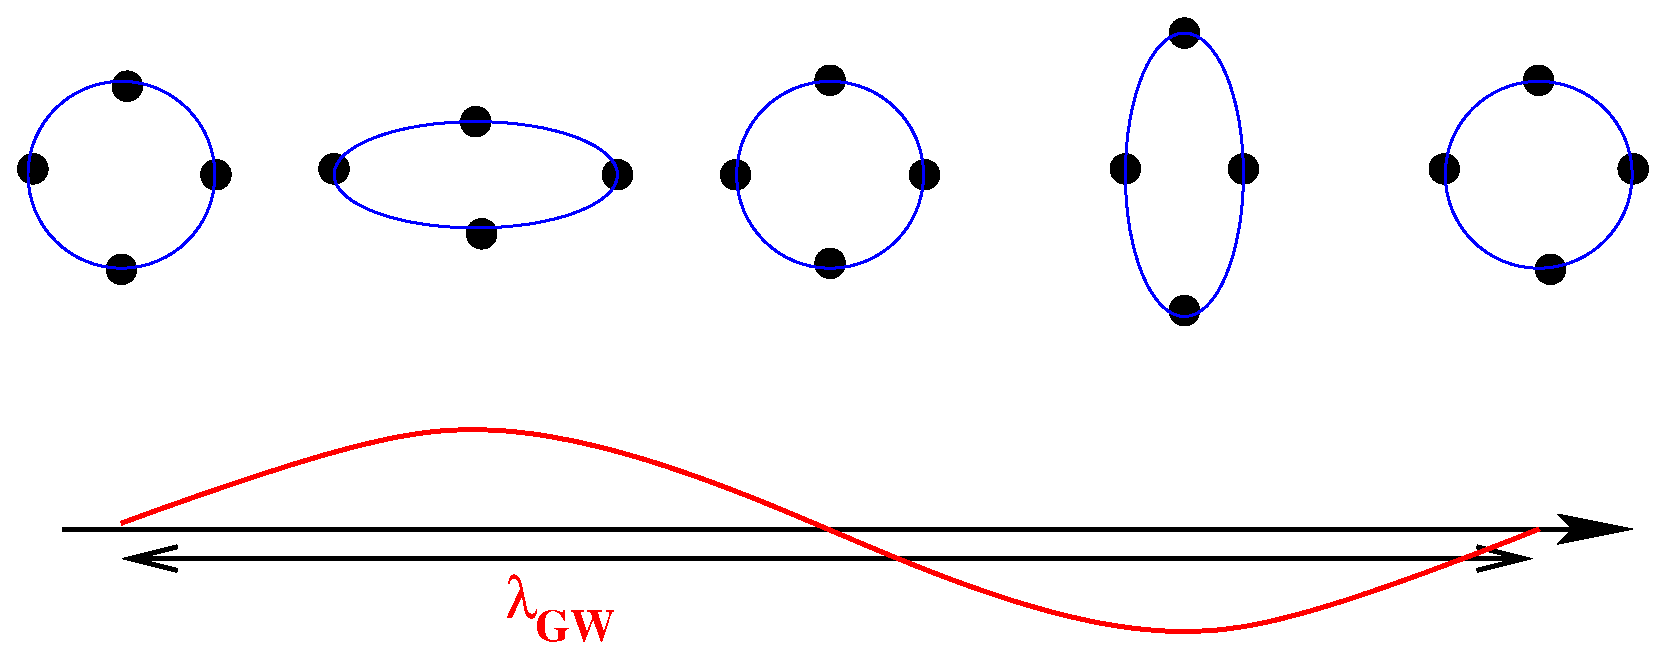
\includegraphics[width=.95\linewidth]{intro/GW1}
\end{subfigure}
\begin{subfigure}{.80\textwidth}
  \centering
  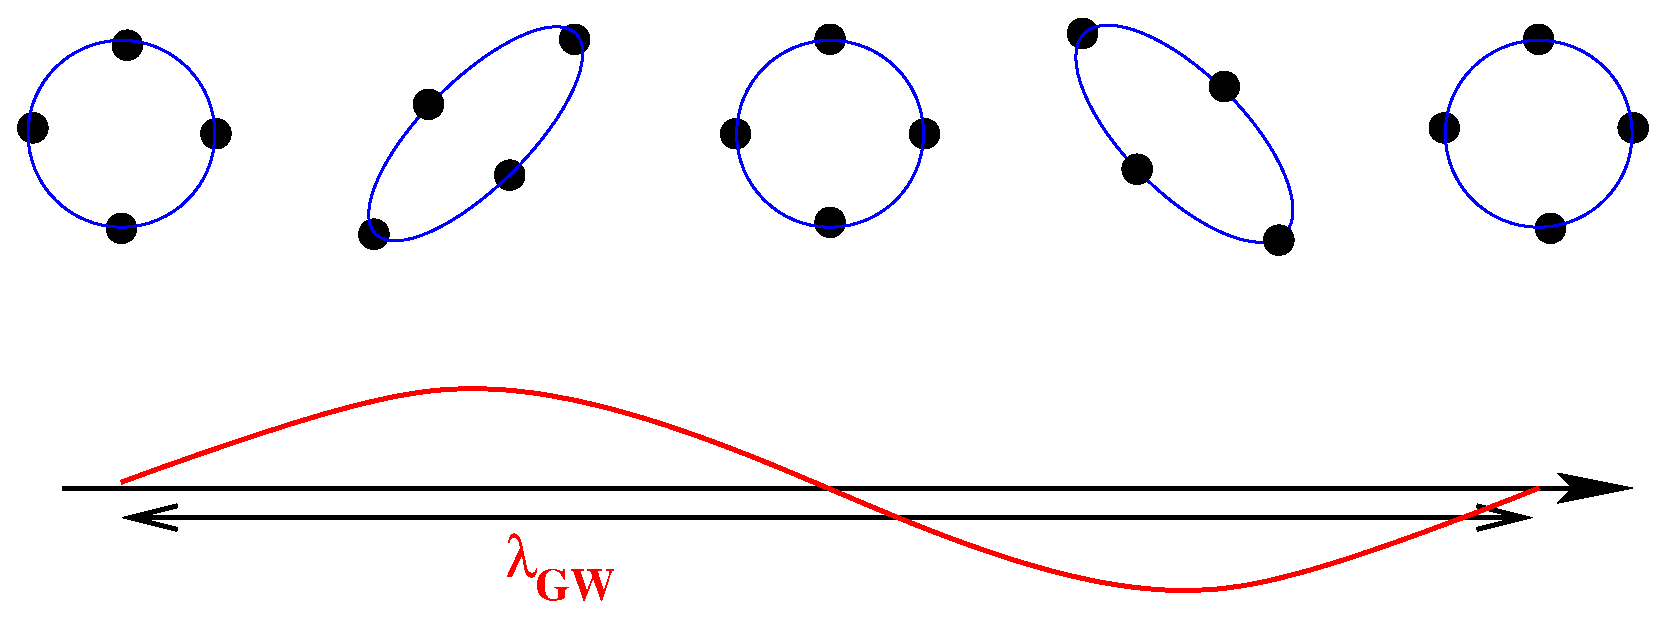
\includegraphics[width=.95\linewidth]{intro/GW2}
\end{subfigure}
\caption[Effect of $+$ and $\times$ polarized gravitational waves on a ring of particles.]{From~\cite{Buonanno:2007yg}. The top panel shows the effect of a $+$ polarized gravitational wave passing through a ring of particles, in the direction perpendicular to the plane of the ring. The bottom panel shows the effect of a $\times$ polarized gravitational wave.}
\label{fig:GWRing}
\end{figure}

When a matter source is present, the wave equation becomes
\begin{equation}
\nabla_{\rho}\nabla^{\rho}h_{\munu}=-16\pi T_{\munu}.
\end{equation}
The solution to this equation can be written with the help of a Green's function,
\begin{equation}
h_{\munu}(t,x^{i})=4\int{d^3y\frac{1}{|x-y|}T_{\munu}(t_r,y^i)},
\end{equation}
where $t_r$ is the ``retarded'' time, $t_r=t-|x-y|$. This integral can be evaluated in terms of the quadruople tensor $I^{ij}$ defined by
\begin{equation}
I^{ij}(t)=\int{d^3x x^ix^jT^{00}(t,x^i)},
\end{equation}
and the reduced quadrupole moment
\begin{equation}
J_{ij}=I_{ij}-\frac{1}{3}\eta_{ij}I,
\end{equation}
where $I=I^{\mu}_{\mu}$.
The result is
\begin{equation}
h_{ij}(t,x^i)=\frac{2}{r}\ddot{J}_{ij}^{\ttt}(t_r)
\end{equation}
In other words, linear gravitational waves are sourced by an oscillating quadrupole. To study the energy content of these gravitational waves, note that the effective stress-energy tensor of this spacetime is
\begin{equation}
T_{\munu}=\frac{1}{32\pi}\left<\partial_{\mu}h_{ij}\partial_{\nu}h^{ij}\right>.
\end{equation}
where $<>$ denotes an appropriate averaging. This can be integrated to find the energy output per unit time in gravitational waves,
\begin{eqnarray}
\label{eq:LGW}
L_{GW}&=&\frac{r^2}{16\pi}\oint{\left<\dot{h}_{\times}^2+\dot{h}_{+}^2\right>d\Omega}\\
&=&\frac{1}{5}\left<\dddot{J}_{ij}^{\ttt}\dddot{J}^{\ttt ij}\right>.
\end{eqnarray}
Let us now consider a circular binary with total mass $M$, reduced mass $\mu$, separation $R$ and orbital frequency $\omega$. Direct computation of the quadrupole tensor gives the simple result
\begin{equation}
L_{GW}=\frac{32}{5}\mu^2M^3R^{-5}.
\end{equation}
Using this, along with the Newtonian estimates $\omega=M^{1/2}R^{-3/2}$, $E=-\frac{\mu M}{2R}$, $dE/dt=-L_{\rm GW}$, allows us the compute the characteristic inspiral scales. The binary shrinks at a rate
\begin{equation}
\frac{dR}{dt}=\frac{dE/dt}{dE/dr}=\frac{-64}{5}M^2\mu R^{-3}.
\end{equation}
Integrating this expression gives the time to coallescence where $R=0$ as
\begin{equation}
\tau_{c}=\frac{5}{256}M^{-2}\mu^{-1}R^{4}.
\end{equation}
As the binary separation decreases, the orbital frequency increases. By integrating
\begin{equation}
\frac{df_{\rm{GW}}}{dt}=\frac{1}{\pi}\frac{d\omega}{dt}=\frac{-3M^{1/2}}{2}R^{-5/2}\frac{dR}{dt},
\end{equation}
the frequency evolution is given by
\begin{equation}
f_{\rm{GW}}(t) = \frac{\omega}{\pi}=\frac{1}{8\pi}\left(\frac{5}{\mu M^{2/3}(\tau_{c}-t)}\right)^{3/8}.
\end{equation}
The number of gravitational waves cycles, $N=\int{f_{\rm{GW}}dt}$, in a given frequency band $df_{\rm{GW}}$ is given by
\begin{equation}
\frac{dN}{d\log{f_{\rm{GW}}}}=\frac{5}{96\pi}\frac{1}{\left(\pi\mathcal{M}f_{\rm{GW}}\right)^{5/3}},
\end{equation}
where the quantity $\mathcal{M}=\mu^{3/5}M^{2/5}$ is called the ``chirp mass''. The explicit radiation pattern is given by
\begin{eqnarray}
h_{+} &=& \frac{4}{r}\mathcal{M}^{5/3}(2\omega)^{2/3}\cos(2\omega t+\phi)\left(\frac{1+\cos^2\theta}{2}\right), \\
h_{\times} &=& \frac{4}{r}\mathcal{M}^{5/3}(2\omega)^{2/3}\sin(2\omega t +\phi)\cos\theta,
\end{eqnarray}
where $r$ is the distance to the source, $\theta$ is the angle between the observer and the axis normal to the orbital plane of the binary, and $\phi$ is the arbitrary phase of the binary. Detectors are sensitive to the strain $h$, rather than the energy flux, and therefore a factor of $x$ improvement in sensitivity results in a factor of $x^3$ higher event rate (assuming a uniformly placed distribution of sources).

These estimates were all made for a circular binary. If the binary has some eccentricity, $e$, then equation~\ref{eq:LGW} is modified to
\begin{equation}
L_{GW}=\frac{32}{5}\mu^2M^3R^{-5}\left(1+\frac{73}{24}e^2+\frac{37}{96}e^4\right)\left(1-e^2\right)^{-7/2}
\end{equation}
However, eccentriccity is radiated away as the inspiral proceeds. The classic reference of Peters(1964) found that
\begin{equation}
\left<\frac{de}{dt}\right>=-\frac{304}{15}e\frac{\mu M^2}{R^4\left(1-e^2\right)^{5/2}}\left(1+\frac{121}{304}e^2\right).
\end{equation}
Thus even a highly eccentric binary will radiate away its eccentricity and circularize before merger, provided the compact objects started far enough away from each other. Most numerical relativity simulations consider only circularized binaries and use techniques to attempt to get rid of any residual eccentricity.

The equations above in this section are valid only for a slowly-moving, weak-field system. As the system gets closer and closer to merger, these equations become increasingly inacurate. Post-Newtonian theory, by expanding to higher order, allows us to consider binaries with higher orbital frequencies. It is typically written as an expansion in the dimensionless parameter 
\begin{equation}
x=\left(\frac{GM\omega}{c^3}\right)^{(2/3)}.
\end{equation}
The evolution of the orbital phase, for example, can be written as
\begin{equation}
\phi=\frac{-x^{-5/2}}{32\nu}\left(1+a_1x + a_2x^{3/2} + a_3x^2 + a_4x^{5/2} + a_5x^3 + a_6x^{7/2}+\mathcal{O}(1/c^8)\right)
\end{equation}
where $\nu$ is the symmetric mass ratio, $\nu=\frac{m_1m_2}{(m_1+m_2)^2}$, and each of the $a_i$ are functions only of $\nu$ and $\log{x}$. This expression is said to be known to 3.5 Post-Newontian order. Additional contrbutions come in at other PN orders, such as spin-orbit coupling at 1.5 PN order, spin-spin coupling at 2 PN order and tidal effects at 5 PN order. See \red{cite} for an overview of PN results and methodology.


\section{The initial value problem in Numerical Relativity}
\label{sec:IVP}
From the point of view of numerical relativity, it is natural to use a 3+1 decomposition of space-time. In this section, we will review this process. Given a globally hyperbolic spacetime $(M,g_{\munu})$. We foliate $M$ by a set of $t={\rm const}$ hypersurfaces $\Sigma_t$.
\begin{center}
\begin{figure}[!ht]
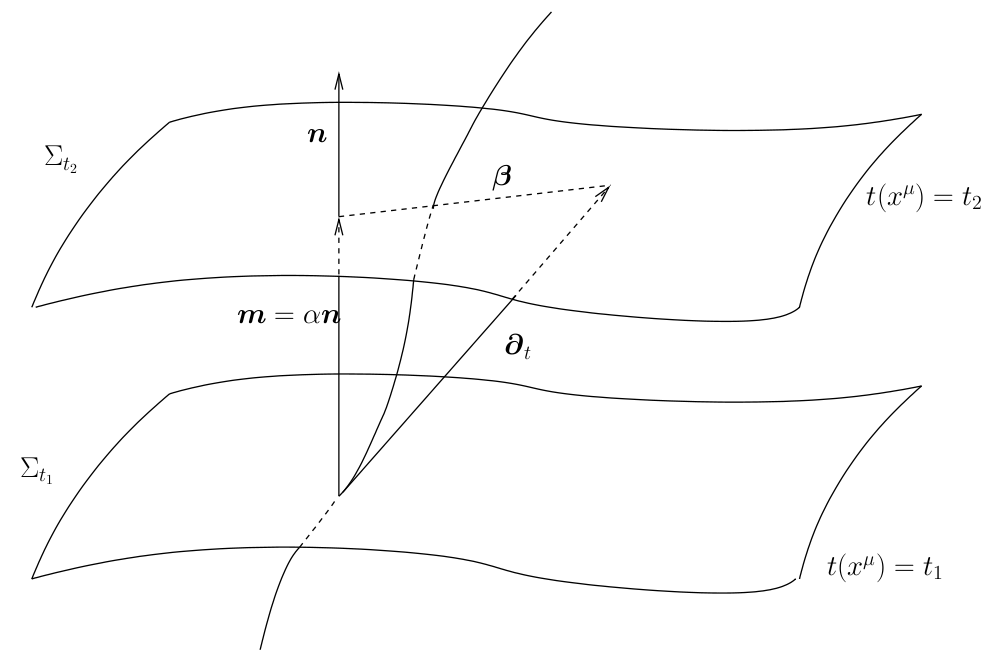
\includegraphics[scale=0.45]{intro/Slice.png}
\label{fig_Slice}
\caption[\red{add caption}]{\red{add caption - from here http://relativity.livingreviews.org/Articles/lrr-2015-1/articlese6.html}}
\end{figure}
\end{center}

 Each surface has a forward pointing unit normal
\begin{equation}
n^{\mu}=-g^{\munu}\nabla_{\nu}t\left(g^{\munu}\nabla_{\mu}t\nabla_{\nu}t\right)^{-1/2},
\end{equation}
induced metric
\begin{equation}
\gamma_{\munu}=g_{\munu}+n_{\mu}n_{\nu},
\end{equation}
and compatible derivative operator $D$.
The induced metric measure curvature inside each hypersurface, while the extrinsic curvature $K_{\munu}$ measures how the hypersurface is curved insde the space-time manifold $M$. It is defined by 
\begin{equation}
K_{\munu}=-\frac{1}{2}\mathcal{L}_{n}g_{\munu},
\end{equation}
where $\mathcal{L}_n$ is the usual Lie derivative, along the direction of the vector field $n^{\mu}$.
The space-time metric is written as
\begin{equation}
ds^2=-\alpha^2dt^2 + \gamma_{ij}\left(dx^i+\beta^idt\right)\left(dx^j+\beta^jdt\right).
\end{equation}
Here $\alpha$ is known as the lapse function - it measures the proper time between neighbouring hypersurfaces. $\beta^i$ is known as the shift - it measures the proper distance within a spatial hypersurface. The lapse and shift are both arbitrary - their choice amounts to a choice of coordinates.

Similar to how Maxwell's equations can be written as a set of constraint equations that do not contain any time derivatives,
\begin{eqnarray}
D_iE^i -4\pi\rho &=& 0, \\
D_iB^i &=& 0,
\end{eqnarray}
and evolution equations,
\begin{eqnarray}
\partial_tE_i&=&\epsilon_{ijk}D^jB^k - 4\pi j_i\\
\partial_tB_i&=&-\epsilon_{ijk}D^jE^k,
\end{eqnarray}
(where $E^i$ is the electric field, $B^i$ is the magnetic field, $\rho$ is the charge density, $j^i$ is the current density, and $\epsilon_{ijk}$ is the Levi-Civitia symbol, and the equations are written in Gaussian units), the same is true of Einstein's equations. The famous Hamiltonian and momentum constraints are
\begin{equation}
R+K^2-K_{ij}K^{ij}=16\pi\rho,
\end{equation}
and,
\begin{equation}
D_{j}K^{j}_{i}-D_iK=8\pi S_i
\end{equation}
where $\rho$ is the energy density measured by a normal observer, $\rho=n_in_jT^{ij}$, and $S_i$ is the momentum density measured by a normal observer $S_i=-\gamma^{j}_in^kT_{jk}$. These are elliptic equations for the geometric quantities defined on the $\Sigma_t$. The general task of constructing initial data is to find ($\Sigma, g_{\munu}, K_{\munu}$) that satisfy the constraint equations and represent well the physical situation at hand (e.g., the inspiral of a compact object binary). The evolution equations are
\begin{equation}
\partial_t\gamma_{ij}=-2\alpha K_{ij} + D_{i}\beta_j + D_j\beta_i
\end{equation}
and
\begin{equation}
\partial_tK_{ij}=-D_iD_j\alpha + \alpha\left(R_{ij}-2K_{ik}K^k_j+KK_{ij}\right)\\
-8\pi\alpha(S_{ij}-\frac{1}{2}\gamma_{ij}(S-\rho))+\beta^kD_kK_{ij}+K_{ik}D_j\beta^k+K_{kj}D_i\beta^k
\end{equation},
where $S_{ab}$ is the spatial stress, $S_{ab}=\gamma^c_a\gamma^d_bT_{cd}$, and $S$ is its trace. Once constraint satisfying initial data has been constructed, the evolution equations determine the geometric quantities at all future times. Analytically, the evolution equations preserve the constraints, although numerically this may not always be the case. 

There are many sets of data $(g_{\munu},K_{\munu})$ that will satisfy the constraint equations. The task remains, then, to choose this free data appropriately. To do so, one typically begins with a conformal decomposition of the metric,
\begin{equation}
\gamma_{ij}=\Psi^4\tilde{\gamma}_{ij}.
\end{equation}
Here, $\Psi$ is called the conformal factor, and $\tilde{\gamma}_{ij}$ is called the conformal metric. Next we break up the extrinsic curvature into its trace and trace-free parts,
\begin{equation}
K_{ij}=A_{ij}+\frac{1}{3}\gamma_{ij}K.
\end{equation}
The Hamiltonian and Momentum constraints become
\begin{equation}
\tilde{D}^2\Psi-\frac{1}{8}\Psi\tilde{R}-\frac{1}{12}\Psi^5K^2+\frac{1}{8}\Psi^{-5}\tilde{A}_{ij}\tilde{A}^{ij}=-2\pi\Psi^{-5}{\rho}.
\end{equation}
\begin{equation}
{D}_j{A}^{ij}-\frac{2}{3}{D}^iK=8\pi j^i,
\end{equation}

$\tilde{A}^{ij}=\Psi^{-10}A^{ij}$. We now proceed according to the extended conformal thin sandwich formalism. See \red{cite} for a review of the alternative traceless-transverse decomposition. We define 
\begin{equation}
\tilde{u}_{ij}=\partial_t\tilde{\gamma}_{ij},
\end{equation}
and we introduce the scalings
\begin{eqnarray}
\tilde{j}^i &=& \Psi^{10}j^i, \\
\tilde{\rho} &=& \Psi^{8}\rho \\
\tilde{A}^{ij} &=& \Psi^{10} A^{ij}. 
\end{eqnarray}
The Hamiltonian and Momentum constraints constraints can now be viewed as equations for the shift and conformal factor
\begin{equation}
\tilde{D}^2\Psi-\frac{1}{8}\Psi\tilde{R}-\frac{1}{12}\Psi^5K^2+\frac{1}{8}\Psi^{-7}\tilde{A}_{ij}\tilde{A}^{ij}=-2\pi\Psi^{-3}\tilde{\rho},
\end{equation}
\begin{equation}
\tilde{D}_j\left(\frac{1}{2\tilde{\alpha}}\left(\mathbb{L}\beta\right)^{ij}-\tilde{D}_j\left(\frac{1}{2\tilde{\alpha}}\tilde{u}^{ij}\right)\right)-\frac{2}{3}\Psi^6\tilde{D}^iK=8\pi\tilde{j}^i,
\end{equation}
where
\begin{equation}
\tilde{\alpha}=\Psi^6\alpha
\end{equation}
is the conformal lapse and 
\begin{equation}
\left(\tilde{\mathbb{L}}\beta\right)^{ij}=\Psi^4\left(D^i\beta^j+D^j\beta^i-\frac{2}{3}\gamma^{ij}D_k\beta^k\right)
\end{equation}
is the conformal longitudinal operator. The lapse is given by the evolution equation of $K$,
\begin{eqnarray}
&&\tilde{D}^2\left(\tilde{\alpha}\Psi^7\right) -
\left(\tilde{\alpha}\Psi^7\right)\bigg[\frac{1}{8}\tilde{R}+\frac{5}{12}\Psi^4K^2+\frac{7}{8}\Psi^{-8}\tilde{A}_{ij}\tilde{A}^{ij}\nonumber \\
\label{eq:XCTS-Lapse}
&&+2\pi\Psi^{-2}\big(\tilde{E}+2\tilde{S}\big)\bigg]=-\Psi^5\left(\partial_{t}K
- \beta^{k}D_kK\right).
\end{eqnarray}
The free data are $\tilde{\gamma}_{ij},\tilde{u}_{ij},K,\partial_tK$. In a coordinate system corotating with the binary, it is natural to choose $\tilde{u}_{ij}=0, \partial_tK=0$. Common choices are conformal flatness, $\tilde{\gamma}_{ij}=\delta_{ij}$ and maximal slicing $K=0$. With appropriate boundary conditions, the system of equations can now be solved.

\section{Binary Neutron Star Systems}
\label{sec:BNS}

%\subsection{Binary Neutron Star Formation}
To begin our discussion of the properties of binary neutron star binaries, we should first briefly review how these system forms. We follow the discussion outlined in \cite{Postnov:2014tza}. The standard formation scenario is illustrated in figure~\ref{fig_BinaryEvolution}, and goes as follows:

\begin{itemize}

\item We begin with two high mass OB main-sequence stars undergoing standard binary evolution. Eventually the more massive (primary) star burns its central hydrogen, and a helium core is left over. 

\item The primary star then rapidly expands, overflows its Roche lobe, and begins a period of mass transfer onto the secondary star. This period lasts until most of the primary's Hydrogen envelope has been transferred, leaving behind a naked helium core.

\item The primary star eventually collapses as a core-collapse supernova, leaving behind a neutron star. It is likely that the explosion disrupts the binary, but let us assume that it survives. We then have a massive main sequence star in orbit with a neutron star.

\item Eventually the secondary star evolves off the main sequence, expands, and overflows its Roche lobe. It will then begin accreting mass onto the primary. This accretion spins up the neutron star, thus ``recycling" it. It also leads to strong x-ray emission.

\item The secondary further expands and a common envelope stage ensues. Eventually the secondary explodes as a supernova, and becomes a neutron star.

\item If the system is not disrupted, it can then become a binary that will eventually merge due to the continuous emission of gravitational waves.

\end{itemize}

\begin{figure}[!ht]
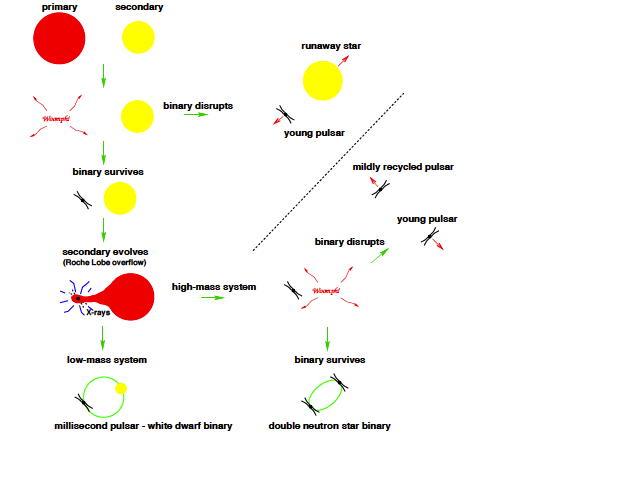
\includegraphics[scale=0.95]{intro/BinaryEvolution.png}
\label{fig_BinaryEvolution}
\caption[Evolutionary scenarios of a typical high-mass binary.]{From \cite{Lorimer2008}. The possible evolutionary scenarios of a typical high mass binary are shown.}
\end{figure}

As discussed earlier, such systems are expected to be quasi-circular once they enter the LIGO band. There are, however, other ways of forming systems that are highly eccentric while in the LIGO band. For example, the dynamical capture in a close two-body encounter in a dense cluster environment, or a binary in a hierarchichal triple system whose eccentricity is enhanced by the Kozai mechanism. Nonetheless, quasi-circular binaries are expected to constitute the large majority of gravitational wave sources.

%NS-NS binaries, unlike BH-BH and BH-NS binaries, have been observed and studied within our galaxy, and therefore the expectations of ground-based gravitational wave detectors for NS-NS binaries are more tightly constrained. The known binary neutron star population is summarized in table~\ref{tab:KnownBNS}
%We report the spin periods, orbital periods, eccentricities, characteristic ages ($\tau_c=P/\dot{P}$), time until coalescence through gravitational wave emission, $\tau_g$. For systems that merge in a Hubble time, we also list the final spin of the star, $P_f$. Assuming magnetic dipole spin-down from a constant magnetic field, this is given by 
%\begin{equation}
%P_f = P\sqrt{1+\frac{\tau_g}{\tau_c}}.
%\end{equation}
% \begin{table}
% \centering
%\label{tab:KnownBNS}
% \caption{The properties of known double neutron star systems}
% \begin{tabular}{c || c | c | c | c | c | c}
% \hline
% System & $P(ms)$ & $P_{\textnormal{orb}}(d)$ & $e$ & $\log_{10}{\tau_c(yr)}$ & $\log_{10}{\tau_g(yr)}$ & $P_f(ms)$ \\
% \hline \hline
% J0737-3039 & 22.7 & 0.102 & 0.088 & 8.3 & 7.9 & 26.8 \\
% J0737-3039 &  2770 & 0.102 & 0.088 & 7.7 & 7.9 &   4453 \\
% J1518+4904 & 40.9 & 8.6 & 0.25 & 10.3 & 12.4 & --- \\
% B1534+12 & 37.9 & 0.32 & 0.27 & 8.4 & 9.4 & 126 \\
% J1756-2251 & 28.5 & 0.32 & 0.18 & 8.6 & 10.2 & --- \\
% J1811-1736 & 104.2 & 18.8 & 0.83 & 9.0 & 13.0 & --- \\
% B1820-11 & 279.8 & 357.8 & 0.79 & 6.5 & 15.8 & --- \\
% J1829+2456 & 41.0 & 1.18 & 0.14 & 10.1 & 10.8 & --- \\
% J1906+0746 & 144.1 & 0.17 & 0.085 & 5.1 & 8.5 & 7224 \\
% B1913+16 & 59.0 & 0.3 & 0.62 & 8.0 & 8.5 & 120 \\
% B2127+11C & 30.5 & 0.3 & 0.67 & 8.0 & 8.3 & 52.6 \\ 
% \end{tabular}
 %\end{table}

The end state of a binary neutron star merger depends strongly on the properties of the stars. For systems with a combined mass less than the maximum mass allowed by the EOS, the final result would be a more massive neutron star. Otherwise, the final result will be a single Kerr black hole. Simulations have shown that these black holes will have a spin on the order of $\chi \simeq 0.6-0.8$. The intermediate state is known as a hypermassive neutron star (HMNS). This is a NS whose mass is above the maximum mass allowed by the EOS, temporarily supported by differential rotation and thermal pressure. Over time, angular momentum is efficiently transported out of the system, and it collapses into a black hole. We can further subdivide these systems based on the timescale for callapse - prompt collapse or delayed collapse. In the prompt case, the pressure support is too low, and the system collapses on a $\sim$ freefall timescale. This is expected in systems with a large total mass ($\gtrsim 2.8M_{\odot}$), although the details depend, of course, on the EOS. In the delayed collapse case, the collapse timescale depends on many factors. Angular momentum distribution by magnetic winding is an important factor - it operates on the Alfven timescale $\tau \sim R\sqrt{\rho}/B \simeq 10-100{\rm ms}$. Transport driven by magneto-rotational instability is also important. It is of the order $\tau \sim 100{\rm ms}$ for $B \simeq 10^{15}G$. Cooling by neutrino or electromagnetic emission is also important, as it decreases thermal pressure, although it operates on a longer timescale, $\sim$ seconds. An accretion disk around the eventual BH, lying beyond the ISCO, will form, with a mass of $\simeq 0.01-0.3 M_{\odot}$. The amount of material in the disk depends on the time to BH formation, as there is more time to distribute angular momentum ot the disk. HMNS systems emit gravitational waves at peak frequencies of approximately $2-4 {\rm kHz}$, unfortunately outside of the optimal frequency range of ground-based detectors. The mass ratio of the system is another important factor. Figure ~\ref{fig:Contours} shows the post-merger remnant of an equal-mass system, and of a system with mass ratio $q\sim 1.38$. The equal mass system shows a ``dumbell''-like structure, composed of two cores which, over time, turn into an ellipsoidal HMNS. The non-equal-mass case shows two asymmetric cores, which act like the smaller one orbiting the larger one. The stronger tidal forces in this case cause the outher layers of the smaller star to be stripped off and form an envelope around the HMNS. Higher disk mass correlates with higher deviations from $q=1$, as well as with higher NS compactness.

\begin{figure}[!t]
\centering
\begin{subfigure}{.80\textwidth}
  \centering
  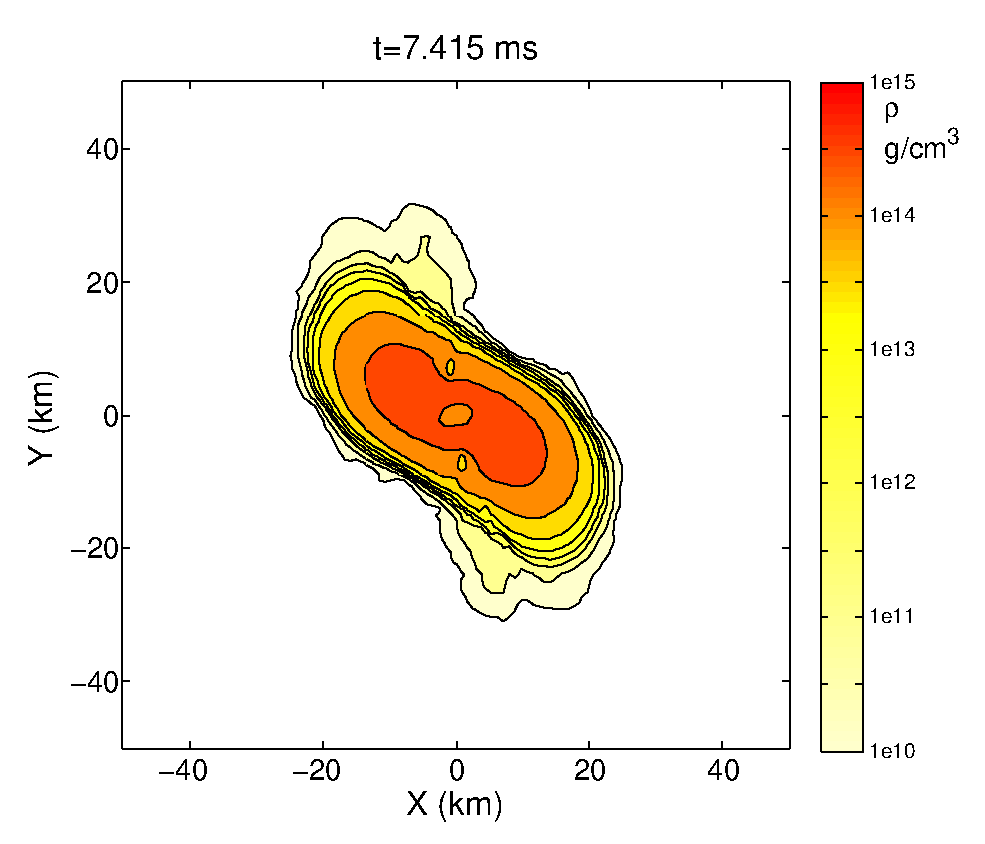
\includegraphics[width=.95\linewidth]{intro/Contours1}
\end{subfigure}
\begin{subfigure}{.80\textwidth}
  \centering
  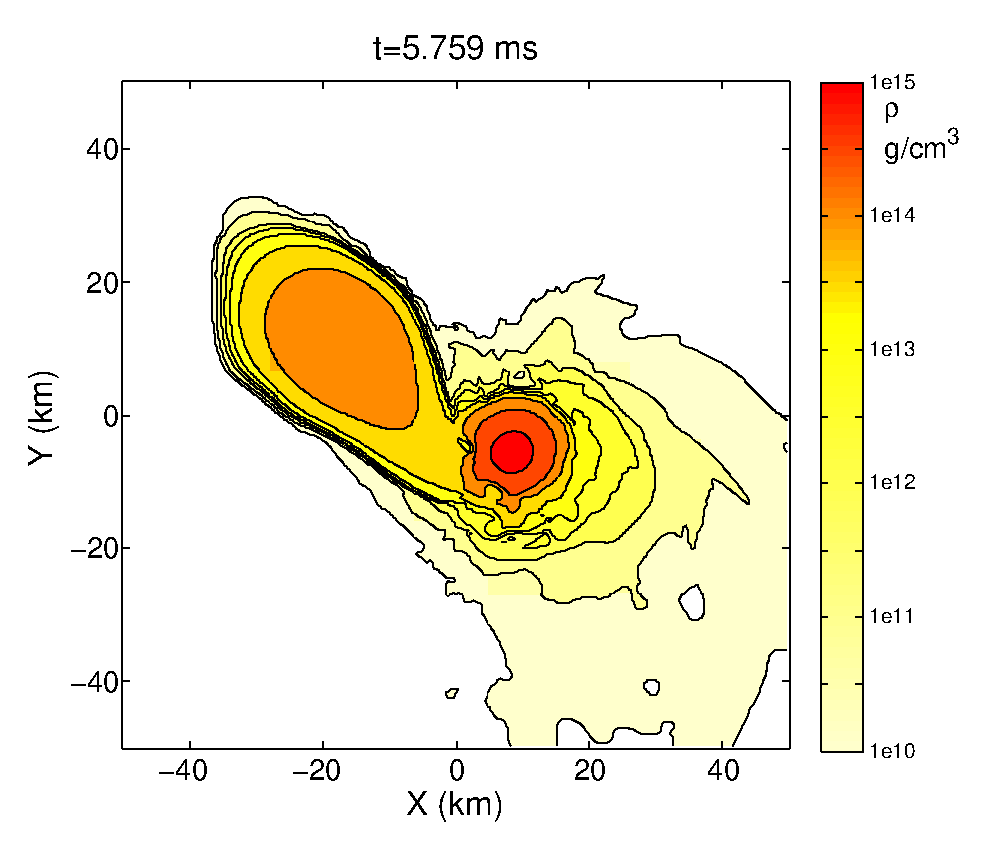
\includegraphics[width=.95\linewidth]{intro/Contours2}
\end{subfigure}
\caption[Comparison of iso-density contours of an equal mass system and a non-equal mass system.]{From ~\cite{Rezzolla:2010fd}. The top panel shows the iso-density contours of the HMNS from an equal mass system with baryon masses $M_1=M_2=1.643M_{\odot}$. The bottom panel shows the iso-density contours of the HMNS from a system with baryon masses $M_1=1.304M_{\odot}$ and $M_2=1.805M_{\odot}$.}
\label{fig:Contours}
\end{figure}

The merger of two neutron stars is the site of the emission of a tremendous amount of electromagnetic energy. Their mergers are thought to be one of the most promising candidates to be the progenitors of short gamma ray bursts (SGRBs), although there is not yet definitive evidence of it. The engine of a rotating black hole, surrounded by a hot accretion torus and a collimiated magnetic field contains the necessary ingreidients thought to be needed for a SGRB. Apart from this, another promising candidate for electromagnetic signature is the ``kilonova'' - emission powered by the radioactive decay of r-process elements formed in the merger, lasting on the time-scale of $\sim$ weeks. Multi-messenger astronomy (see \cite{Fan:2015bia} for a review) seeks to combine information from gravitational waves, these electromagnetic events, and possible neutrino observations, to further elucidate the astrophysics of these mergers.

One of the most exciting prospects of the Advanced LIGO era is using gravitational wave observations to constrain the NS EOS. The EOS of dense nuclear matter is an open question of tremendous interest to nuclear physicists and astrophysicists alike. Tidal effects are parameterized by the tidal deformability paramter $\lambda$, which relates the induced quadrupole field of one star, $Q_{ij}$, to the tidal field in which it is immersed, $\mathcal{E}_{ij}$:
\begin{equation}
Q_{ij}=-\lambda(m;{\rm EOS})\mathcal{E}_{ij}.
\end{equation}
Or, likewise, by the second tidal Love number,
\begin{equation}
k_2=\frac{3}{2}\frac{\lambda}{R^5}.
\end{equation}
These enter the PN equations for binary phase at the very high 5PN order, but because of the large pre-factors, they are still very important in the late-stage inspiral dynamics. Much work has been done to estimate how well Advanced LIGO can measure these paramters (see ~\cite{Read2009b,Hinderer2010,damour:12,Lackey2011}). \cite{DelPozzo:13} (further extended in~\cite{Agathos:2015a}) used a Bayesian framework to show that $\lambda$ could be constrained at the 10\% level after a few tens of detections. There is also the question of more exotic NS matter. \cite{Chatziioannou:2015uea} studied various possibilities and found, for example, that a detection with an SNR of $\sim 20$ could provide good evidence of the existence or non-existence of strange quark stars. However, kaon condensates or hyperons in NS cores are much more difficulty to confirm.

Numerical simulations of the mergers of binary neutron stars have been possible for at least fifteen years \red{cite}. Since then, simulations have rapidly progressed, adding more resolution, more orbits, more detailed physics, and a better coverage of the available paramter space. \red{Cite a bunch of papers here, on those different things}. With the great increase in simulation technology, and the coincident start of the Advanced LIGO era, it is truly an exciting time for this field.

%\section{Astrophysical Motivation}

%\subsection{How Important is Spin?}
%The obvious first question to ask is, ``what spin is necessary to be relevant in a binary neutron star simulation?" After answering that, we will then ask, ``are there realistic astrophysical scenarios that would produce such spins?''

%Our first approach is just a simple comparison of time scales. The two relevant time scales in the problem are the orbital period, $P_{\textnormal{orb}}$, and the spin period, $P$. If $P_{\textnormal{orb}}\ll P$, then the spin can be safely neglected, but if this condition is false, then the spin may be important. Kepler's third law gives
%\begin{equation}
%P_{\textnormal{orb}}^2=\frac{4\pi^2a^3}{M}
%\end{equation}
%Suppose the neutron stars are close to merger, say, $a=45km$. If we take $M=2.8M_{\odot}$, then the orbital period is $P_{\textnormal{orb}}\approx 3ms$. If the $\ll$ criterion is taken to be an order of magnitude, we can then conclude that neutron stars with a spin period on the order of a few dozen milliseconds might be non-negligible.

%Next, we can investigate how much the neutron star spin can affect the accumulated orbital phase of the system. Consider an equal mass system, where one of the neutron stars has dimensionless spin $\chi=\frac{J}{M^2}$ aligned with the orbital momentum. Boyle et. al. (2007)\cite{BoyleEtAl2007} gives the accumulated phase difference, due to spin-orbit coupling, computed at 2.5 Post-Newtonian order, as a function of $x=a/M$ as
%\begin{equation}
%\Phi\approx -\chi\left(\frac{1.22}{x}-8.5\log{x}\right)
%\end{equation}
%If we want to compute the phase error accumulated in LIGO's most sensitive region for binary neutron stars, say 40Hz-400Hz \cite{AndersonCreighton2008}, this corresponds to finding the difference between $x=0.0144$ and $x=0.067$. The result is
%\begin{equation}
%\delta\Phi \approx -80\chi
%\end{equation}
%The error in the waveform phase is just twice the orbital phase,
%\begin{equation}
%\delta\phi \approx -160\chi
%\end{equation}
%If we take the neutron star's angular momentum to be $J=\frac{2}{5}MR^2\Omega$, then its dimensionless spin is
%\begin{equation}
%\chi = \left(\frac{R}{15km}\right)^2\left(\frac{1.4M_{\odot}}{m}\right)\left(\frac{1ms}{P}\right)
%\end{equation}
%and the phase error is then
%\begin{equation}
%\delta\phi = 10rad \left(\frac{R}{15km}\right)^2\left(\frac{1.4M_{\odot}}{m}\right)\left(\frac{16ms}{P}\right)
%\end{equation}

%Finally, let us make a crude estimate on the effect of the disk mass after the merger due to neutral star spin. This can crudely be done by assuming all of the spin angular momentum of the neutron star goes into the disk, i.e., we set
%\begin{equation}
%J_{NS} = J_{D}
%\end{equation}
%\begin{equation}
%\frac{4\pi}{5}\frac{M_{NS}R_{NS}^2}{P} = \frac{1}{2}M_DR_D^2\Omega_{D}
%\end{equation}
%Let's assume that the remnant mass is $2M_{NS}$ and that $R_D=fM_{\textnormal{Remnant}}$ for some real number $f$. We then obtain that the disk mass is
%\begin{equation}
%M_D = \frac{4\pi}{5\sqrt{f}}\frac{R_{NS}^2}{P}
%\end{equation}
%If we take $f=6$ as for non-rotating black holes, we obtain
%\begin{equation}
%M_D = 0.005M_{\odot}\left(\frac{R}{15km}\right)^2\left(\frac{P}{10ms}\right)^{-1}
%\end{equation}
%This mass could easily be enhanced by adding a small deviation away from equal mass ratio, and give the mass necessary to be the engine of short GRBs.

%Although these are not completely precise arguments, the take away message here should be that neutron stars with spins on the order of a couple tens of milliseconds should not be neglected in simulations.

%\subsection{Binary Neutron Star Formation}
%To begin our discussion of the properties of binary neutron star binaries, we should first briefly review how these system forms. We follow the discussion outlined in \cite{PostnovYungelson2006}. The standard formation scenario is illustrated in figure 1courtesy of \cite{Lorimer2008}, and goes as follows:

%\begin{itemize}

%\item We begin with two high mass OB main-sequence stars undergoing standard binary evolution. Eventually the more massive (primary) star burns its central hydrogen, and a helium core is left over. 

%\item The primary star then rapidly expands, overflows its Roche lobe, and begins a period of mass transfer onto the secondary star. This period lasts until most of the primary's Hydrogen envelope has been transferred, leaving behind a naked helium core.

%\item The primary star eventually collapses as a core-collapse supernova, leaving behind a neutron star. It is likely that the explosion disrupts the binary, but let us assume that it survives. We then have a massive main sequence star in orbit with a neutron star.

%\item Eventually the secondary star evolves off the main sequence, expands, and overflows its Roche lobe. It will then begin accreting mass onto the primary. This accretion spins up the neutron star, thus ``recycling" it. It also leads to strong x-ray emission.

%\item The secondary further expands and a common envelope stage ensues. Eventually the secondary explodes as a supernova, and becomes a neutron star.

%\item If the system is not disrupted, it can then become a binary that will eventually merge due to the continuous emission of gravitational waves.

%\end{itemize}

%\begin{figure}[!ht]
%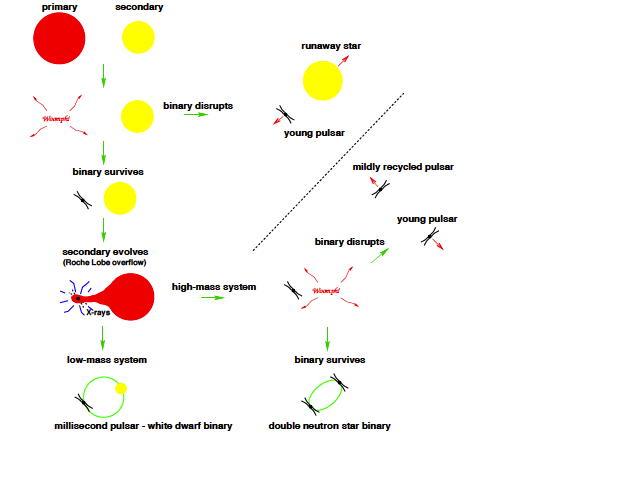
\includegraphics[scale=0.75]{intro/BinaryEvolution.png}
%\label{fig_BinaryEvolution}
%\caption{Courtesy of \cite{Lorimer2008}. The possible evolutionary scenarios of a typical high mass binary are shown}
%\end{figure}

%\subsection{Why Corotation is Unphysical}
%In principle, neutron stars in compact binaries could perhaps be spun up to coronation by tidal torques. The argument that they are not is outlined in \cite{BildstenCutler1992}. Consider a binary consisting of a neutron of mass $m$ and radius $R$, with a companion (either a neutron star or black hole) of mass $M$. Let $a$ be their semi-major axis, and suppose the induced tidal bulge is misaligned with the orbital separation by an angle $\alpha$. Then the tidal torque on the neutron star is 
%\begin{equation}
%N \leq \frac{M^2R^5\sin{2\alpha}}{2a^6}
%\end{equation}
%Let's suppose that the maximum torque is being continuously exerted, i.e., $\sin{2\alpha}=1$. The orbital separation where synchronization can first occur is
%\begin{equation}
%a_{\textnormal{synch}}\leq\frac{M^2m^2}{400\left(M+m\right)^3}\left({R}{m}\right)^6
%\end{equation}
%If we wish to impose that synchronization occurs before tidal disruption, this constrains the radius of the neutron star to be
%\begin{equation}
%\frac{R}{m}\geq4\left(\frac{M}{m}\right)^{4/15}\left(1+\frac{m}{M}\right)^{2/3}
%\end{equation}
%Or, $R\geq 13km$ for an equal mass, $M=1.4M_{\odot}$ binary. This shows that even the maximum amount of tidal torquing is not very effective. Now let us go further and assume that rather than maximum torque, the neutron star has some finite viscosity. The lag angle, $\alpha \ll 1$, is related to the viscous damping time by
%\begin{equation}
%\alpha \approx \frac{\Omega_{\textnormal{orb}}}{t_{\textnormal{visc}}\omega_0^2}
%\end{equation}
%where $\Omega_0$ is the natural response frequency, $\omega_0^2\approx\frac{M}{R^3}$. This can be parametrized by a parameter $\beta$ as $t_\textnormal{visc}=\frac{R}{\beta}$, so that $\beta=1$ represents a light crossing time. It is then calculated that the value of $\beta$ required for tidal locking before reaching the tidal radius
%\begin{equation}
%\beta\geq\frac{60\left(M+m\right)^{5/3}}{Mm^{2/3}}\left(\frac{m}{R}\right)^3
%\end{equation}
%This becomes $\beta\geq 1.6$ for a typical binary neutron star system, and $\beta\geq 2.4$ for a typical black hole neutron star system. Reasonable estimates for neutron star viscosity fall far below this. In other words, dense matter is not nearly viscous enough for tidal locking to occur. For example, \cite{Kochanek1992} finds  that a typical crust viscosity is $10^{28}g\,cm^{-1}s^{-1}$, while the viscosity required for tidal locking here trantes to $2\times10^{31}\beta\,g\,cm^{-1}s^{-1}$.

%\subsection{The Known Binary Neutron Star Population}
%We now discuss the properties of the known galactic binary neutron star population. This is summarized in \cite{PostnovYungelson2006}.
%Table 1 shows the relevant properties of the neutron stars in the nine known systems. We list the name of the system, the spin period of the pulsar, $P$, its eccentricity, $e$, its characteristic age, $\tau_c$, and the time until coalescence through gravitational gravitational wave emission, $\tau_g$. The characteristic age is related to the pulsar's period derivative, $\dot{P}$, by
%\begin{equation}
%\tau_c = \frac{P}{2\dot{P}}
%\end{equation}
%and the gravitational wave time is given by \cite{PostnovYungelson2006}
%\begin{equation}
%\tau_g \simeq 4.8\times 10^{10} yr \left(\frac{P_{\textnormal{orb}}}{day}\right)^{8/3}\left(\frac{m1+m2}{M_{\odot}}\right)^{-2/3}\left(\frac{\mu}{M_{\odot}}\right)^{-1}\left(1-e^2\right)^{7/2}
%\end{equation}
% For systems that merge in a Hubble time, we also list the final spin of the pulsar, $P_f$. Assuming magnetic dipole spin down from a constant magnetic field, this is given by \cite{ShapiroTeukolsky}
% \begin{equation}
% P_f  = P\sqrt{1+\frac{\tau_g}{\tau_c}}
% \end{equation}
 
 %\begin{center}
 %\begin{table}
 %\caption{The properties of known double neutron star systems}
 %\begin{tabular}{c || c | c | c | c | c | c}
 %\hline
 %System & $P(ms)$ & $P_{\textnormal{orb}}(d)$ & $e$ & $\log_{10}{\tau_c(yr)}$ & $\log_{10}{\tau_g(yr)}$ & $P_f(ms)$ \\
 %\hline \hline
 %J0737-3039 & 22.7 & 0.102 & 0.088 & 8.3 & 7.9 & 26.8 \\
 %J0737-3039 &  2770 & 0.102 & 0.088 & 7.7 & 7.9 &   4453 \\
 %J1518+4904 & 40.9 & 8.6 & 0.25 & 10.3 & 12.4 & --- \\
 %B1534+12 & 37.9 & 0.32 & 0.27 & 8.4 & 9.4 & 126 \\
 %J1756-2251 & 28.5 & 0.32 & 0.18 & 8.6 & 10.2 & --- \\
 %J1811-1736 & 104.2 & 18.8 & 0.83 & 9.0 & 13.0 & --- \\
 %B1820-11 & 279.8 & 357.8 & 0.79 & 6.5 & 15.8 & --- \\
 %J1829+2456 & 41.0 & 1.18 & 0.14 & 10.1 & 10.8 & --- \\
 %J1906+0746 & 144.1 & 0.17 & 0.085 & 5.1 & 8.5 & 7224 \\
 %B1913+16 & 59.0 & 0.3 & 0.62 & 8.0 & 8.5 & 120 \\
 %B2127+11C & 30.5 & 0.3 & 0.67 & 8.0 & 8.3 & 52.6 \\ 
 %\end{tabular}
 %\end{table}
 %\end{center}
 
 %The most striking system in this table is the first pulsar in the system, J0737-3039. With a period of just 26.8ms at merger,  this pulsar may not be able to be accurately modelled as irrotational, based on our previous arguments. At the very least, it gives a good indication that there are probably other systems out there with even lower periods, which cannot be well-modelled as irrotational.

%\subsection{Population Synthesis}
%Because we know of so few binary neutron star systems that will merge in a Hubble time, we are ultimately largely limited by small number statistics. Population synthesis models give another way to understand what sort of spin distribution is expected in binary neutron stars, although these models are ultimately limited by a lack of understanding in the initial parameters of the system, and in the physical processes that occur between the first supernova and the second. In this section, we discuss the recent results of the population synthesis study of \cite{OslowskiEtAl2011}.

%The parameters of the model are an initial magnetic field drawn logarithmically from $B\in\left[10^{11}G,10^{13}G\right]$ an initial pulsar spin period of $10ms$, a radius $R=10km$ and moment of inertia $I=10^{45} gcm^2$ for all pulsars. There is also a magnetic field time decay scale $\tau_d$, so that $B$ decays exponentially to a value $B_{\textnormal{min}}=10^8G$. Timescales of $\tau_d = 5Myr, 20Myr, 1Gyr, 2Gyr$ are all used in different models. There are different accretion models as well - a standard one, and one in which hypercritical Bondi-Hoyle accretion occurs during the common envelope phase. The mass accreted in this model is roughly 10 times that of the standard accretion model, although the authors assume that the neutron star does not spin up in  this phase. 

%Skipping ahead to the results, the output of each model is mapped onto a $P-\dot{P}$ diagram, while accounting for observational biases so that the map can be compared to radio surveys and thus the likelihood of each model can be evaluated. Two models of interest are the models $SP$ and $HP$ which are plotted in figure 2. Model HP allows for hypercritical accretion during the common envelope phase, and model SP uses a different IMF for the newly formed neutron stars.

%\begin{centering}
%\begin{figure}[!ht]
%\label{fig_PopSynth}
%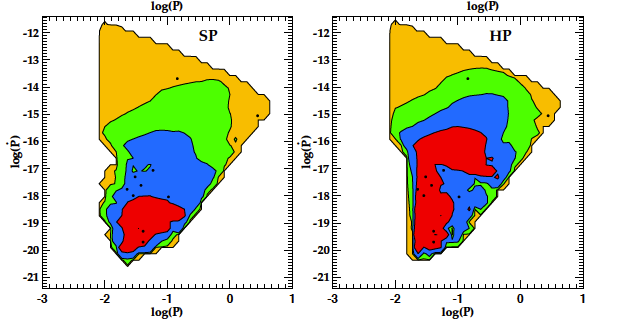
\includegraphics[scale=0.75]{intro/PopSynth.png}
%\caption{Courtesy of~\cite{OslowskiEtAl2011}. Shows the $P-\dot{P}$ distribution for two possible models.}
%\end{figure}
%\end{centering}

%Although these plots are not an exact representation of the actual binary population, as radio observation effects are taken into account, the takeaway is that there are models which can produce a large number of pulsars with $P\sim 10ms$, and $\dot{P}\sim 10^{-19}-10^{-20}$. With $\dot{P}$ that low, the pulsar would essentially have the same spin if it merged in 1Gyr or so. Furthermore, these models match up well on the $P-\dot{P}$ diagram with the known binary population. It appears that the hard edge on the low period side of the graphs is an artifact of the selection of all pulsars starting at $10ms$ - perhaps a more realistically modelled distribution would allow for even lower spin pulsars. Although these models are ultimately disfavoured to another model without as many low $\dot{P}$ pulsars by a further comparison to the chip mass distribution of known systems, based on all the free parameters and uncertainty involved in the study it seems reasonable to think that these models are physically plausible.

%\subsection{Hypercritical Accretion}
%We'll say a brief word on hypercritical accretion. During the common envelope phase, it is possible for super-Eddington accretion to be powered by neutrino losses. Although this process has been studied in the literature (see \cite{Chevalier1996} for example), the physical processes involved are quite complicated and uncertain. In is unclear whether or not this is a viable mechanism to produce millisecond pulsars, or whether black hole formation is inevitable due to the high mass gain. However, this is at least a plausible to produce highly spinning stars in neutron star binaries, and thus provides further motivation to study them.

%\section{Contemporary Research}
%\label{sec_PrevWork}
%Although as mentioned betore, corotation is an unphysical assumption, studies which have compared corotational configurations to irrotational configurations can still give us insight into the effects that highly spinning neutron stars can have on the dynamics of the system. We now review several studies that have done such comparisons.

%Shibata and Uryu (1999)\cite{ShibataUryu2000} simulated equal-mass mergers, with a $\Gamma=2$ equation of state using quasi-equilibrium initial data sequences starting very close to the merger. There was an extremely large difference found in the disk mass: For corotational configurations, a disk of mass $0.05-0.1M_{\odot}$ can be formed, whereas for irrotational configurations, the disk mass was $< 0.01M_{\odot}$. The merger remnant for two comparable configurations is shown in figure 3.

%\begin{centering}
%\begin{figure}[!ht]
%\label{fig_Shibata}
%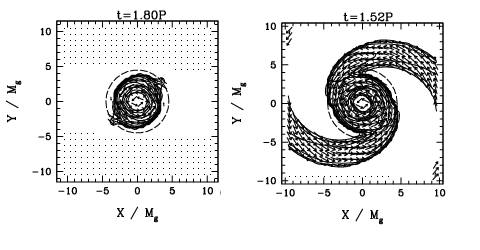
\includegraphics[scale=0.75]{intro/ShibataUryu.png}
%\caption{Courtsey of \cite{ShibataUryu2000}. A comparison of the disks formed from irrotational and corotational configurations.}
%\end{figure}
%\end{centering}

%Faber and Rasio (2000)\cite{FaberRasio2000} compared corotational and irrotational configurations using a Post-Newtonian SPH code. The results are qualitatively similar to Shibata and Uryu: corotation leads to a much more prominent disk.

%Duez et. al. (2002)\cite{DuezEtAl2002} focused on the inspiral phase, and the effect of corotation versus irrotation on the gravitational waveform. The result, simply stated, is that the amplitude of the waveform is the same at a given separation, but the corotational inspirals proceeds much quicker - It took the irrotational configuration 96.6 wave cycles to go from $r=10.8M$ to $r=6.78M$ compared to 62.1 cycles to go from $r=10.8M$ to $r=6.75M$ for the corotational configuration.

%Oechslin et. al. (2007)\cite{OechslinEtAl2007} used an SPH code which uses the conformal flatness approximation to general relativity. Interestingly, not only did they use corotational configurations with aligned spins, but also anti-aligned, oppositely aligned, and tilted spin configurations. The qualitative results are, again, that corotation leads to a much larger disk than irrotation ($0.21M_{\odot}$ compared to $0.04M_{\odot}$) for the Shen equation of state. Also, it is found that counterrotation severely suppresses the disk, and that tilted configurations have disk sizes similar to the aligned case.

\chapter[BNS with Arbitrary Spins in Numerical Relativity]{Binary Neutron Stars with Arbitrary Spins in Numerical Relativity}
\label{chap:bns}

{\it The material in this chapter is based on ''Binary neutron stars with arbitrary spins in numerical relativity" by Nick Tacik et al. Phys. Rev. D 92, 124012, December 2015. The material in the appendix of this chapter is based on an erratum to that article, submitted to Phys. Rev. D.} 

\section{Chapter Summary}
 We present a code to construct initial data for binary neutron star
  systems in which the stars are rotating. 
  Our code, based on a formalism
  developed by Tichy, allows for arbitrary rotation axes of the
  neutron stars and is able to achieve rotation rates near rotational
  breakup. We compute the neutron star angular momentum through quasilocal angular momentum
    integrals. When constructing irrotational binary neutron stars, we find a very small residual dimensionless spin of $\sim 2\times 10^{-4}$. Evolutions of rotating neutron star binaries show that the magnitude of the
    stars' angular momentum is conserved, and that the spin and
    orbit precession of the stars is well described by
    post-Newtonian approximation. We demonstrate that orbital
  eccentricity of the binary neutron stars can be controlled to
  $\sim 0.1\%$. The neutron stars show
    quasinormal mode oscillations at an amplitude which increases
    with the rotation rate of the stars.
\section{Introduction}



Several known binary neutron star (BNS) systems  will merge within a
Hubble time due to inspiral driven by gravitational
radiation~\citep{Lorimer2008}, most notably the Hulse-Taylor
pulsar~\citep{Hulse:1975uf}. Therefore, binary neutron stars
constitute one of the prime targets for upcoming gravitational wave
detectors like Advanced LIGO~\citep{aLIGO1,aLIGO2} and Advanced
Virgo~\citep{AdV,TheVirgo:2014hva}.
The neutron stars in known binary pulsars have fairly long rotation
periods~\citep{Lorimer2008}. The system J0737-3039~\citep{Lyne:2004cj}
contains the fastest known spinning neutron star in a binary with a
rotation period of 22.7ms. This system will merge within $\sim
10^8$~years through gravitational wave driven inspiral. Globular
clusters contain a significant fraction of all known milli-second
pulsars~\citep{Lorimer2008}, which through dynamic interactions, may
form binaries~\citep{2010ApJ...720..953L,Benacquista:2011kv}. Gravitational wave driven
inspiral reduces~\citep{PetersMathews1963,Peters1964} the initially
high eccentricity of dynamical capture binaries.
Given the presence of milli-second pulsars in
globular clusters, dynamically formed BNS may contain very rapidly
spinning neutron stars with essentially arbitrary spin orientations.
Presence of spin in BNS systems does influence the evolution of the
binary. For instance, in order to avoid a loss in sensitivity in gravitational wave (GW)
searches, one needs to account for the NS spin~\citep{Brown:2012qf}.
Furthermore, early BNS simulations~\citep{Shibata00b} of irrotational
and corotational BNS systems found that the spin
of corotating BNS noticeably increased the size of accretion discs
occurring during the merger of the two NS. The properties of
accretion discs and unbound ejecta are intimately linked to
electromagnetic and neutrino emission from merging compact object
binaries~\citep{metzger:11}. 
Understanding the behavior of rotating BNS systems is therefore important to quantify the expected observational signatures from such systems.
These considerations motivated a recent interest in the numerical
modeling of rotating binary neutron star systems during their last
orbits and coalescence.~\cite{Baumgarte:2009fw},~\cite{Tichy:2011gw}, and~\cite{East:2012zn} presented formalisms for constructing BNS
initial data for spinning neutron stars. Tichy proceeded to construct
rotating BNS initial data~\citep{Tichy:2012rp}; and~\cite{Bernuzzi:2013rza} studies short inspirals and mergers of
BNS with rotation rates consistent with known binary neutron stars
(i.e. a dimensionless angular momentum of each star
$\chi=S/M^2\lesssim 0.05$), and rotation axes aligned with the orbital
angular momentum. Very recently,~\cite{Dietrich:2015pxa} presented a comprehensive study of BNS, including a simulation of a precessing, merging BNS.~\cite{East:2015yea} investigate
interactions of rotating neutron stars on highly eccentric orbit.
~\cite{Kastaun:2013mv} determine the maximum spin of the
black hole remnant formed by the merger of two aligned spin rotating
neutron stars.~\cite{Tsatsin:2013jca} present
initial data and evolutions for non-spinning, spin-aligned and
anti-aligned data sets.~\cite{Tsokaros:2015fea} presented initial data and quasi-equilibrium sequences
of spin-aligned and anti-aligned binaries with a nuclear equation of state.

Previous studies differ in the type of initial data used:~\citep{Baumgarte:2009fw,Tichy:2011gw,Tichy:2012rp,Bernuzzi:2013rza}
construct and utilize constraint-satisfying initial data, which also
incorporates quasi-equilibrium of the binary system.
~\cite{East:2012zn,East:2015yea} construct constraint-satisfying
data based on individual Tolman-Oppenheimer-Volkof (TOV) stars, without regard of preserving
quasi-equilibrium in the resulting binary, but providing greatly
enhanced flexibility in the type of configurations that can be
studied, e.g. hyperbolic encounters.
~\cite{Kastaun:2013mv,Tsatsin:2013jca}, finally, only
approximately satisfy the constraint equations.
Previous studies also
differ in the rigor with which the neutron star angular momentum is
measured.~\cite{Tichy:2012rp} merely discusses the neutron stars
based on a rotational velocity $\omega^i$ entering the initial data
formalism (cf. our Eq.~(\ref{eq:UniformRotation}) below), whereas~\citep{Bernuzzi:2013rza,Kastaun:2013mv,East:2015yea} estimate the
initial neutron star spin either based on single star models or based
on the differences in binary neutron star initial data sets with and
without rotation, and thus neglecting the impact of interactions in
the binary. All these studies measure the neutron star angular
momentum in the initial data. Changes in the neutron star angular
momentum that could happen during initial
relaxation of the binary or during the subsequent evolution of the
binary are not monitored.

In this chapter we study the construction of rotating binary neutron
star initial data and the evolution through the inspiral phase. We
implement the constant rotational velocity (CRV) formalism developed
in~\cite{Tichy:2012rp}, and construct constraint satisfying BNS
initial data sets with a wide variety of spin rates, as well as different spin
{\it directions}. We apply quasilocal angular momentum techniques
developed for black holes to our BNS initial data sets; the
quasilocal spin indicates that we are able to construct BNS with
dimensionless angular momentum exceeding 0.4. Evolving some of the
constructed initial data sets through the inspiral phase, we
demonstrate that we can control and reduce orbital eccentricity by an
iterative adjustment of initial data parameters controlling orbital
frequency and radial velocity of the stars, both for non-precessing
(i.e. aligned-spin binaries) and precessing binaries. When monitoring
the quasi-angular momentum of the neutron stars during the inspiral,
we find that its magnitude is conserved, and the spin-direction
precesses in a manner consistent with post-Newtonian predictions.

This chapter is organized as follows. Section~\ref{sec:Methodology}
describes the initial data formalism and our numerical code to solve
for rotating BNS initial data. In Sec.~\ref{sec:ID} we use this
code to study a range of initial configurations, 
with a special emphasis on the behavior of
the quasilocal spin diagnostic. We evolve rotating BNS in
Sec.~\ref{sec:EvolutionResults}, including a discussion of
eccentricity removal, the behavior of the quasilocal spin
diagnostics, and a comparison of the precession dynamics to
post-Newtonian theory. A discussion concludes the chapter in
Sec.~\ref{sec:Discussion}. In this chapter, we work in units where $G=c=M_{\odot}=1$.

%%%%%%%%%%%%%%%%%%%%%%%%%%%%%%%%%%%%%%%%%%%%%%%%%%%%%%%%%%%%%%%%
\section{Methodology}
\label{sec:Methodology}
%%%%%%%%%%%%%%%%%%%%%%%%%%%%%%%%%%%%%%%%%%%%%%%%%%%%%%%%%%%%%%%%

\subsection{Formalism for Irrotational Binaries}
\label{sec:IrrotFormalism}

To start, we will review a formalism commonly used for the 
construction of initial data for system of irrotational binary neutron stars. 
We will then discuss how to
build upon this formalism to construct initial data for neutron stars
with arbitrary spins.

We begin with the 3+1 decomposition of the space-time metric
(see~\cite{2007gr.qc.....3035G} for a review),
\begin{equation}
ds^2 = -\alpha^2 dt^2 + \gamma_{ij}\left(dx^i +
\beta^idt\right)\left(dx^j + \beta^jdt\right).
\end{equation}

Here, $\alpha$ is the lapse function, $\beta^i$ is the shift vector
and $\gamma_{ij}$ is the 3-metric induced on a hypersurface
$\Sigma(t)$ of constant coordinate time $t$. In this decomposition, the unit normal
vector $n^{\mu}$ to $\Sigma(t)$ and the tangent vector $t^{\mu}$ to
the coordinate line $t$ are related by
\begin{equation}
t^{\mu} = \alpha n^{\mu} + \beta^{\mu},
\end{equation}
with $n_\mu=(-\alpha,0,0,0)$ and $\beta^\mu=(0,\beta^i)$. The
extrinsic curvature of $\Sigma(t)$ is the symmetric tensor defined as
\begin{equation}
K_{\mu\nu} = -\nabla_\nu n_\mu -n_\nu \gamma^\lambda_{\phantom{\lambda}\mu} \nabla_\lambda (\ln \alpha) =
-\frac{1}{2}\mathcal{L}_n \gamma_{\mu\nu},
\end{equation}
where $\gamma_{\mu \nu}=g_{\mu \nu} + n_\mu n_\nu$ is the extension of
the 3-metric $\gamma_{ij}$ to the 4-dimensional spacetime, and $g_{\mu
  \nu}$ is the 4-metric of that spacetime. By construction, $K^{\mu
  \nu}n_\mu =0$ and we can restrict $K^{\mu \nu}$ to the 3-dimensional
tensor $K^{ij}$ defined on $\Sigma \times \Sigma$. The extrinsic
curvature $K^{ij}$ is then divided into its trace $K$ and trace-free
part $A^{ij}$:
\begin{equation}
K^{ij} = A^{ij} + \frac{1}{3}\gamma^{ij}K.
\end{equation}

We treat the matter as a perfect fluid with stress-energy tensor
\begin{equation}
T_{\mu\nu} = \left(\rho+P\right)u_{\mu}u_{\nu} + Pg_{\mu\nu},
\end{equation}
where $\rho=\rho_0 (1+\epsilon)$ is the energy density, $\rho_0$ the
baryon density, $\epsilon$ the specific internal energy, $P$ the
pressure, and $u_\mu$ the fluid's 4-velocity. For the initial value
problem, it is often convenient to consider the following projections
of the stress tensor:
\begin{eqnarray}
E &=& T^{\mu\nu}n_{\mu}n_{\nu}, \\ S &=&
\gamma^{ij}\gamma_{i\mu}\gamma_{j\nu}T^{\mu\nu},\\ J^{i} &=&
-\gamma^{i}_{\phantom{i}\mu}T^{\mu\nu}n_{\nu}.
\end{eqnarray}

We then further decompose the metric according to the conformal
transformation
\begin{equation}
\gamma_{ij} = \Psi^4\tilde{\gamma}_{ij}.
\end{equation}
Other quantities have the following conformal
transformations:
\begin{eqnarray}
E &=& \Psi^{-6}\tilde{E}, \\ S &=& \Psi^{-6}\tilde{S}, \\ J^{i} &=&
\Psi^{-6}\tilde{J}^i, \\ A^{ij} &=& \Psi^{-10}\tilde{A}^{ij},\\ \alpha
&=& \Psi^{6}\tilde{\alpha}.
\end{eqnarray}

$\tilde{A}^{ij}$ is related to the shift and the time derivative of the conformal
metric, $\tilde{u}_{ij}=\partial_t\tilde{\gamma}_{ij}$ by
\begin{equation}
\tilde{A}^{ij} =
\frac{1}{2\tilde{\alpha}}\left[\left(\tilde{\mathbb{L}}\beta\right)^{ij}-\tilde{u}^{ij}\right],
\end{equation}
where $\tilde{\mathbb{L}}$ is the conformal longitudinal operator whose action on a vector $V^i$ is
\begin{equation}
\left(\tilde{\mathbb{L}}V\right)^{ij} = \tilde{\nabla}^iV^j +
\tilde{\nabla}^jV^i -
\frac{2}{3}\tilde{\gamma}^{ij}\tilde{\nabla}_kV^k,
\end{equation}
and $\tilde{\nabla}$ is the covariant derivative defined with respect to 
the conformal 3-metric $\tilde \gamma_{ij}$.

In the 3+1 formalism, the Einstein equations are decomposed into a set
of evolution equations for the metric variables as a function of $t$,
and a set of constraint equations on each hypersurface
$\Sigma(t)$. The initial data problem consists in providing quantities
$g_{\mu \nu}(t_0)$ and $K_{\mu \nu}(t_0)$ which satisfy the
constraints on $\Sigma(t_0)$ and represent initial conditions with the
desired physical properties (e.g. masses and spins of the objects,
initial orbital frequency, eccentricity, etc.).We solve the constraint
equations using the Extended Conformal Thin Sandwich (XCTS)
formalism~\citep{York1999}, in which the constraints take the form of
five nonlinear coupled elliptic equations. The XCTS equations can be
written as

\begin{equation}
2\tilde{\alpha}\bigg[\tilde{\nabla}_j\left(\frac{1}{2\tilde{\alpha}}\big(\tilde{L}\beta\big)^{ij}\right)-\tilde{\nabla}_j\left(\frac{1}{2\tilde{\alpha}}\tilde{u}^{ij}\right)
\label{eq:XCTS-Shift}
-\frac{2}{3}\Psi^6\tilde{\nabla}^iK-8\pi\Psi^4\tilde{J}^i\bigg]=0,
\end{equation}

\begin{equation}
\tilde{\nabla}^2\Psi - \frac{1}{8}\Psi\tilde{R} -
\frac{1}{12}\Psi^5K^2
\label{eq:XCTS-ConformalFactor}
+\frac{1}{8}\Psi^{-7}\tilde{A}_{ij}\tilde{A}^{ij} +
2\pi\Psi^{-1}\tilde{E}= 0,
\end{equation}

\begin{eqnarray}
&&\tilde{\nabla}^2\left(\tilde{\alpha}\Psi^7\right) -
\left(\tilde{\alpha}\Psi^7\right)\bigg[\frac{1}{8}\tilde{R}+\frac{5}{12}\Psi^4K^2+\frac{7}{8}\Psi^{-8}\tilde{A}_{ij}\tilde{A}^{ij}\nonumber \\
\label{eq:XCTS-Lapse}
&&+2\pi\Psi^{-2}\big(\tilde{E}+2\tilde{S}\big)\bigg]=-\Psi^5\left(\partial_{t}K
- \beta^{k}\partial_kK\right).
\end{eqnarray}

We solve these equations for the conformal factor $\Psi$, the
densitized lapse $\tilde\alpha\Psi^7$ and the shift $\beta^i$. $\tilde{E}$,
$\tilde{S}$ and $\tilde{J}^i$ determine the matter content of the
slice. The variables $\tilde{\gamma}_{ij}$, $\tilde{u}_{ij} =
\partial_t\tilde{\gamma}_{ij}$, $K$ and $\partial_t K$ are freely
chosen.

  If we work in a coordinate system corotating with the binary,
  $\tilde{u}_{ij} = 0$ and $\partial_t K = 0$ are natural choices for
  a quasi-equilibrium configuration. Following earlier work~\citep{Taniguchi2007,TaniguchiEtAl:2006,FoucartEtAl:2008}, we also choose to
  use maximal slicing, $K=0$, and a conformally flat metric,
  $\tilde{\gamma}_{ij}=\delta_{ij}$. 
  Maximal slicing is a gauge choice that determines the
    location of the initial data hypersurface in the embedding space
    time. Conformal flatness is used for computational convenience;
    rotating black holes are known to be not conformally
    flat~\citep{GaratPrice:2000}, and so this simplifying assumption should be revisited in the future.

In addition to solving these equations for the metric variables, we
must impose some restrictions on the matter. In particular, the stars
should be in a state of approximate hydrostatic equilibrium in the comoving
frame. 
This involves solving the Euler equation and the continuity
equation. For an irrotational binary, the first integral of the Euler
equation leads to the condition
\begin{equation}
h\alpha\frac{\gamma}{\gamma_0} = C,
\label{eq:Euler0}
\end{equation}
where $C$ is a constant, hereafter referred to as the Euler constant, the specific enthalpy $h$ is defined as
\begin{equation}
h = 1+\epsilon + \frac{P}{\rho_0},
\end{equation}
and we have introduced
\begin{eqnarray}
\gamma &=& \gamma_n\gamma_0\left(1 -
\gamma_{ij}U^iU^j_0\right),\\ \gamma_0 &=& \left(1 -
\gamma_{ij}U^i_0U^j_0\right)^{-1/2},\\ \gamma_n &=& \left(1 -
\gamma_{ij}U^iU^j\right)^{-1/2},\\ U^i_0 &=& \frac{\beta^{i}}{\alpha}.
\end{eqnarray}
The 3-velocity $U^i$ is defined by
\begin{eqnarray}
u^{\mu} &=& \gamma_n (n^\mu + U^\mu),\\ U^\mu n_\mu &=& 0.
\end{eqnarray}

The choice of $U^i$, which is unconstrained in this formalism, is an
important component is determining the initial conditions in the
neutron star. For irrotational binaries (non-spinning neutron stars),
there exists a potential $\phi$ such that
\begin{equation}
U^i = \frac{\Psi^{-4}\tilde{\gamma}^{ij}}{h\gamma_n}\partial_j\phi.
\end{equation}
The continuity equation can then be written as a second-order elliptic
equation for $\phi$:
\begin{equation}
\label{eq:Continuity}
\frac{\rho_0}{h}\nabla^{\mu}\nabla_{\mu}\phi +
\left(\nabla^{\mu}\phi\right)\nabla_{\mu}\frac{\rho_0}{h}=0.
\end{equation}

Under the assumption of the existence of an approximate helicoidal Killing vector $\xi$~\citep{Teukolsky:1998sh,Shibata:1998um}, this equation becomes
\begin{align}
\rho_0\,\bigg\{\!\!&-\tilde{\gamma}^{ij}\partial_i\partial_j\phi + 
\frac{h\beta^{i}\Psi^4}{\alpha}\partial_i\gamma_n+hK\gamma_n\Psi^4
\nonumber 
\quad+\left[\tilde{\gamma}^{ij}\tilde{\Gamma}^k_{ij}+\gamma^{ik}\partial_i\left(\ln\frac{h}{\alpha\Psi^2}\right)\right]\partial_k\phi 
\bigg\} \nonumber \\
&=
\tilde{\gamma}^{ij}\partial_i\phi\partial_j\rho_0-\frac{h\gamma_n\beta^i\Psi^4}{\alpha}\partial_i\rho_0. 
\label{eq:Continuity0}
\end{align}

Another simple choice for $U^i$ is to enforce corotation of the star,
i.e. $U^i=U^i_0$. This would be the case if neutron star binaries were
tidally locked. However, viscous forces in neutron stars are expected
to be insufficient to impose tidal locking~\citep{BildstenCutler1992},
and the neutron star spins probably remain close to their value at
large orbital separations.

Once we have obtained $h$ from the metric and $U^i$, the other
hydrodynamical variables can be recovered if we close the system by the
choice of an equation of state for cold neutron star matter in
$\beta$-equilibrium, $P = P(\rho_0)$ and $\epsilon=\epsilon(\rho_0)$.
Throughout this work, we use a polytropic equation of state, $P=\kappa\rho_0^\Gamma$, with $\Gamma=2$. The internal energy, $\epsilon\rho_0$, satisfies 
\begin{equation}
\epsilon\rho_0=\frac{P}{\Gamma-1}.
\end{equation}

The boundary conditions of our system of equations are quite
simple. At the outer boundary of the computational domain (which we
approximate as ``infinity'' and is in practice $10^{10}M_{\odot}$), we require the metric to be Minkowski
in the inertial frame, and so in the corotating frame we have
\begin{eqnarray}
{\bm \beta} &=& {\bm \Omega}_0 \times {\bm r} + \dot a_0 {\bm
  r},\\ \alpha &=& 1,\\ \Psi &=& 1,
\end{eqnarray}
with ${\bm \Omega}_0$ the initial orbital frequency of the binary and
$\dot{a}_0r=\dot{r}$ is the initial infall velocity of the binary (this quantity is negative for an inspiral).
We choose ${\bm
  \Omega}_0=(0,0,\Omega_0)$, with $\Omega_0$ and $\dot{a}_0$ as freely
specifiable variables that determine the initial eccentricity of the
binary.

At the surface of each star, the boundary condition can be easily
inferred from the $\rho_0=0$ limit of equation~(\ref{eq:Continuity0}):
\begin{equation}
\tilde{\gamma}^{ij}\partial_i\phi\partial_j\rho_0 =
\frac{h\gamma_n\beta^{i}\Psi^4}{\alpha}\partial_i\rho_0.
\end{equation}

Finally, we discuss how a first guess for the orbital angular velocity
$\Omega_0$ can be obtained for a non-spinning system. The force
balance equation at the centre of the NS is
\begin{equation}\label{eq:Nablah}
\nabla\ln\left({\frac{h\gamma_0}{\alpha\gamma}}\right)=0.
\end{equation}
Neglecting any infall velocity, this condition guarantees that the
binary is in a circular orbit. This is only an
approximation as there is really some infall velocity, but this still
leads to low eccentricity binaries with $e\sim 0.01$. 
Along with the assumption that the enthalpy is maximal at the centre of the NS,
\begin{equation}
\nabla\ln h=0,
\end{equation}
we can write this condition as
\begin{equation}
\nabla\left(\ln{\frac{\gamma_0}{\alpha\gamma}}\right)=0,
\end{equation}
or, by using the definitions of $\gamma_0$, and $\gamma$,
\begin{equation}
\nabla\ln\left(\alpha^2 - \gamma_{ij}\beta^{i}\beta^{j}\right) =
-2\nabla\ln{\gamma}.
\label{eq:OmegaEq}
\end{equation}
If we decompose $\beta^i$ in its inertial component $\beta^i_0$ and
its comoving component according to
\begin{equation}
{\bm \beta} = {\bm \beta}_0 + {\bm \Omega}_0 \times {\bm r} + \dot a_0
{\bm r},
\end{equation}
this can be written as a quadratic equation for the orbital angular
velocity $\Omega_0$ (neglecting the dependence of $\gamma$ on the
orbital angular velocity $\Omega_0$). In practice, we solve for
$\Omega_0$ by projecting Eq.~(\ref{eq:OmegaEq}) along the line
connecting the center of the two stars.\footnote{Along the other
  directions, the specific enthalpy $h$ is corrected so that force balance is
  enforced at the center of the star, according to the method
  described in~\cite{Foucart:2010eq}}

The exact iterative procedure followed to solve in a consistent manner
the constraint equations, the elliptic equations for $\phi$, and the
algebraic equations for $h$ (including on-the-fly computation of
$\Omega_0$ and of the constant in the first integral of Euler
equation) is detailed in Section~\ref{sec:IDalgorithm}.

Once a quasi-equilibrium solution has been obtained by this method,
lower eccentricity systems can be generated by modifying $\Omega_0$
and $\dot{a}_0$, following the methods developed by~\cite{Pfeiffer-Brown-etal:2007}.

\subsection{Formalism for Spinning Binaries}
We will now discuss how to alter the formalism discussed above to
incorporate spinning BNS. Although several formalisms have been
introduced in the past \citep{Marronetti:2003gk,Baumgarte:2009fw}, we will
follow the work of~\cite{Tichy:2011gw}. A
first obvious difference is that we can no longer write the velocity
solely in terms of the gradient of a potential. Following Tichy, we
break the velocity up into an irrotational part, and a new rotational
part $W$:
\begin{equation}
U^i =
\frac{\Psi^{-4}\tilde{\gamma}^{ij}}{h\gamma_n}\left(\partial_j\phi+W_j\right),
\end{equation}
where it is natural, although not required, for $W$ to be
  divergenceless.

Following the assumptions stated in~\cite{Tichy:2011gw}, the continuity equation becomes
\begin{align}
\rho_0\,\bigg\{\!\!&-\tilde{\gamma}^{ij}\partial_i\big(\partial_j\phi+W_j\big)  + \frac{h\beta^i\Psi^4}{\alpha}\partial_i\gamma_n + hK\gamma_n\Psi^4 \nonumber\\
&\qquad+\Big[\tilde{\gamma}^{ij}\tilde{\Gamma}^k_{ij}+\gamma^{ik}\partial_i\big(\ln \frac{h}{\alpha\Psi^2}\big)\Big] 
\big(\partial_k\phi+W_k\big) \bigg\} \nonumber \\
&=\tilde{\gamma}^{ij}\big(\partial_i\phi+W_i\big)\partial_j\rho_0 - \frac{h\gamma_n\beta^i\Psi^4}{\alpha}\partial_i\rho_0.
\label{eq:Continuity}
\end{align}
Eq.~\ref{eq:Continuity} then is the same as in the irrotational
case, cf. Eq.~\ref{eq:Continuity0}, under the replacement $\partial_i\phi\rightarrow\partial_i\phi+W_i$.

Taking the limit $\rho_0\to 0$ in Eq.~(\ref{eq:Continuity}) yields the
boundary condition at the surface of each star:
\begin{equation}
\tilde{\gamma}^{ij}\left(\partial_i\phi+W_i\right)\partial_j\rho_0=\frac{h\gamma_n\beta^i\Psi^4}{\alpha}\partial_i\rho_0.
\end{equation}

The solution of the Euler equation is no longer as simple as it was
previously, in Eq.~\ref{eq:Euler0}. As
shown in~\cite{Tichy:2011gw}, the solution is
now
\begin{equation}
h = \sqrt{L^2 -
  \left(\nabla_i\phi+W_i\right)\left(\nabla^i\phi+W^i\right)},
\end{equation}
where
\begin{equation}
L^2 =
\frac{b+\sqrt{b^2-4\alpha^4\left(\left(\nabla_i\phi+W_i\right)W^i\right)^2}}{2\alpha^2},
\end{equation}
and
\begin{equation}
b =
\left(\beta^i\nabla_i\phi+C\right)^2+2\alpha^2\left(\nabla_i\phi+w_i\right)w^i.
\end{equation}

Finally, the method discussed previously of modifying the star's
angular velocity is now no longer as simple. The equation is modified
to
 \begin{equation}
\nabla\ln\left(\alpha^2-\gamma_{ij}\beta^{i}\beta^{j}\right)=-2\nabla\ln\Gamma,
\end{equation}
where
\begin{equation}
\Gamma
=\frac{\gamma_n\left(1-\left(\beta^i+\frac{W^i\alpha}{h\gamma_n}\right)\frac{\nabla_i\phi}{\alpha
    h\gamma_n}- \frac{W_i W^i}{\alpha^2\gamma_n^2}\right) } { \sqrt{ 1
    - \left(\frac{\beta^i}{\alpha}+\frac{W^i}{h\gamma_n}\right)
    \left(\frac{\beta_i}{\alpha}+\frac{W_i}{h\gamma_n}\right) } }.
\end{equation}

Let us now discuss the choice of the spin term, $W$. This term is, in
principle, freely chosen, and so we must choose it so as to best
represent the physical situation at hand - namely a uniform rotation
with constant angular velocity. As suggested by~\cite{Tichy:2011gw} and~\cite{Tichy:2012rp}, a reasonable choice for $W$ is 
\begin{equation}
\label{eq:UniformRotation}
W^i = \epsilon^{ijk}\omega^{j}r^k,
\end{equation}
where $r^k$ is the position vector centered at the star's centre,
$\omega^j$ represents an angular velocity vector and $\epsilon^{ijk}=\left\{\pm 1,0\right\}$. This leads to a vector field $W^i$ with vanishing divergence in the conformal metric $\tilde{g}_{ij}=\delta_{ij}$. Alternatively, one might prefer a vector field $V^i$ with vanishing divergence with respect to the physical metric $g_{ij}=\Psi^4\delta_{ij}$. Owing to the conformal transformation properties of the divergence operator, $V^i$ is given by
\begin{equation}
\label{eq:ConformalUniformRotation}
V^i=\Psi^{-6}W^i.
\end{equation}
Here, we generally use $W^i$ as we have found that it leads to initial data which is closer to being in equilibrium, as we will further discuss in section~\ref{sec:QNModes}.


%%%%%%%%%%%%%%%%%%%%%%%%%%%%%%%%%%%%%%%%%%%%%%%%%%%%%%%%%%%%%%%%
\subsection{Solving the Elliptic Equations}
%%%%%%%%%%%%%%%%%%%%%%%%%%%%%%%%%%%%%%%%%%%%%%%%%%%%%%%%%%%%%%%%


\begin{figure}
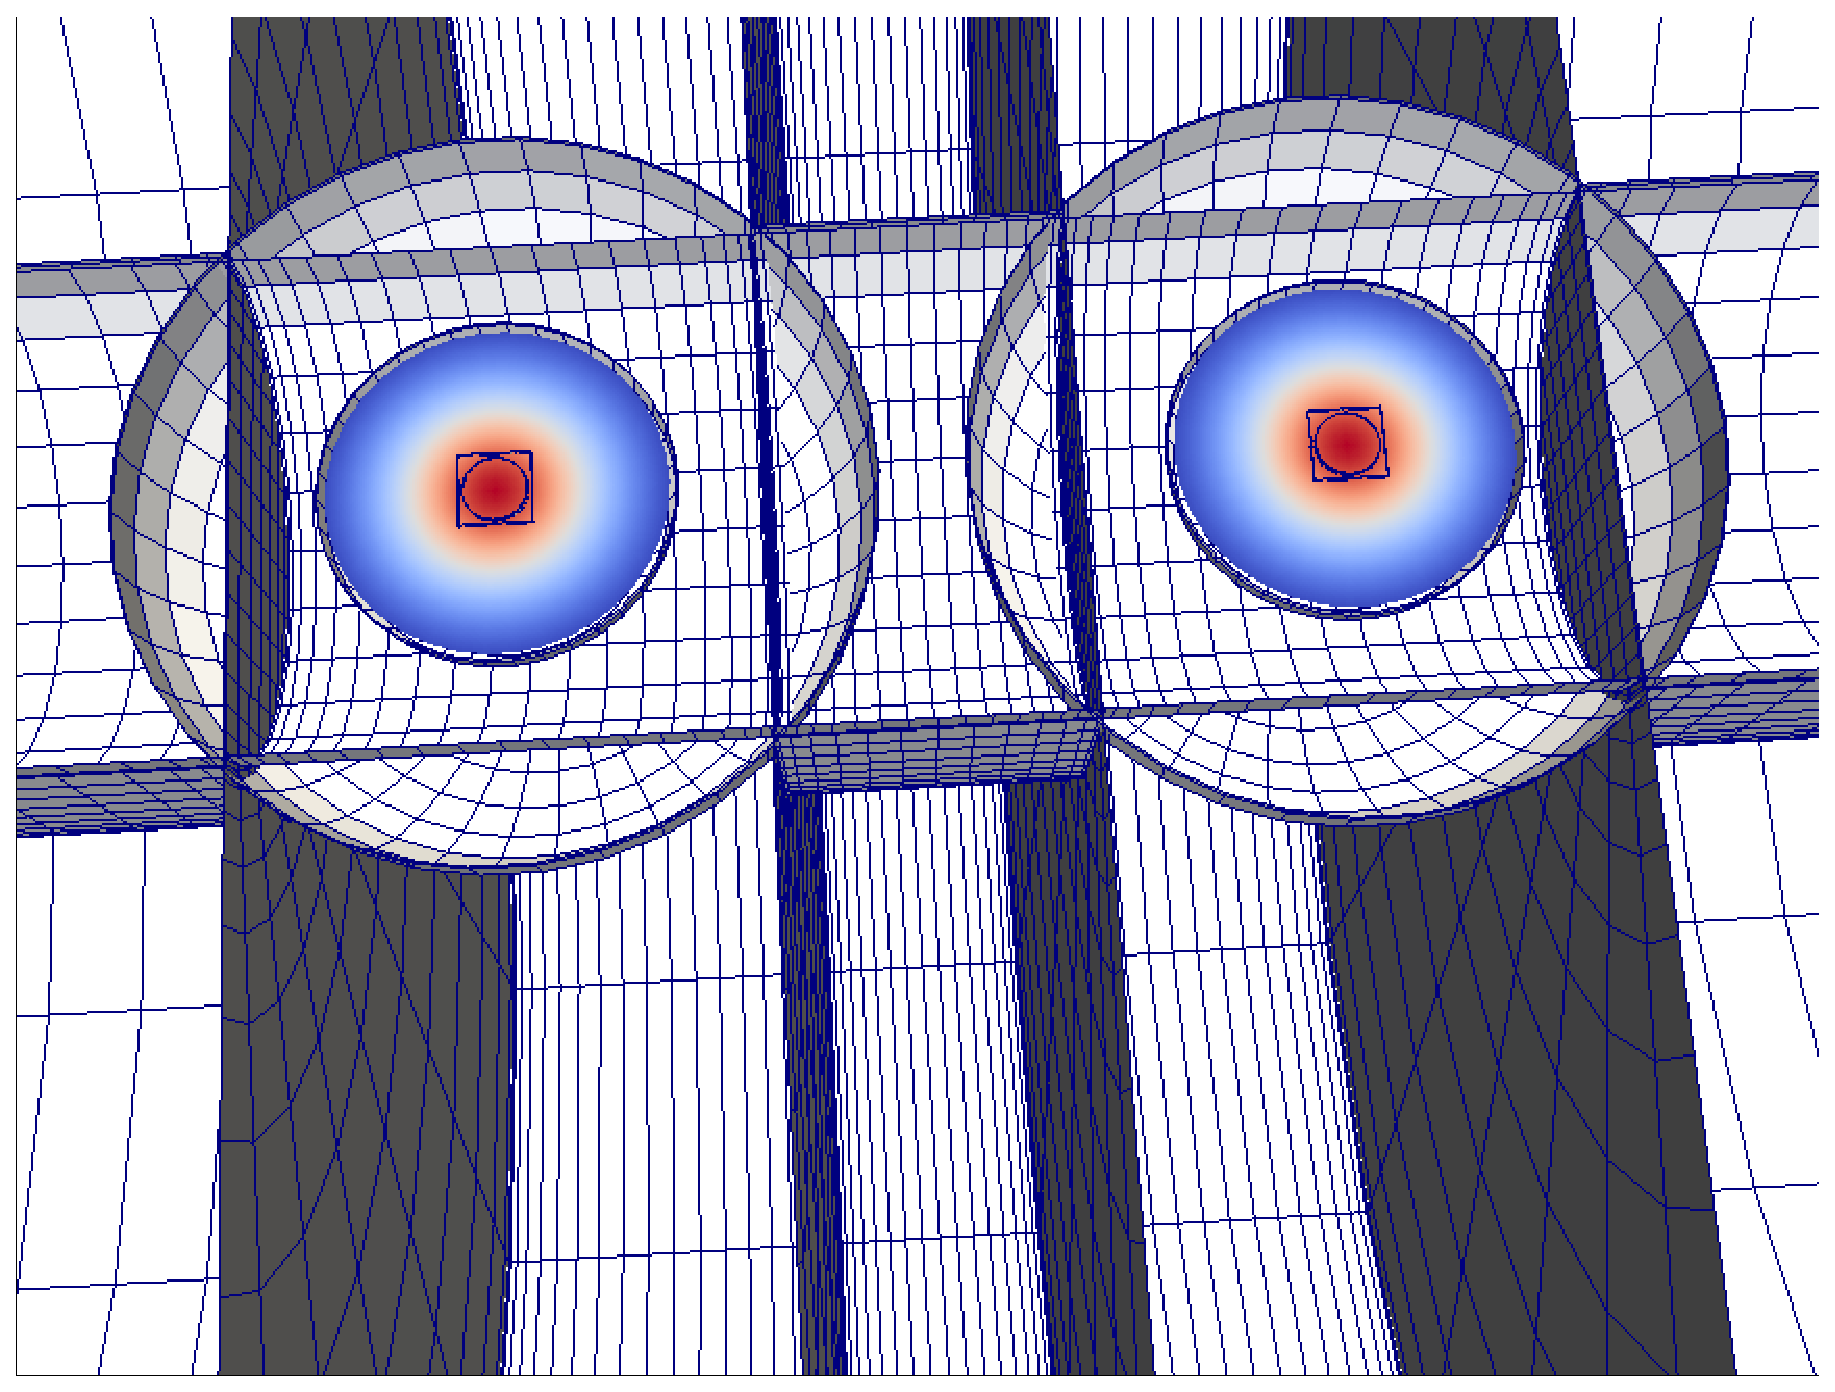
\includegraphics[width=0.95\columnwidth,trim=0 185 0 0, clip=true]{chap2/TheDomain}
\caption[Visualization of the BNS initial data domain decomposition.]{\label{fig:TheDomain} Visualization in the x-y plane of the
  domain decomposition used in our initial data solve. The colour map
  represents the density of the stars. }
\end{figure}

In the previous sections, we have reduced the Einstein
  constraints, Eqs.~(\ref{eq:XCTS-Shift})--(\ref{eq:XCTS-Lapse}), as
  well as the continuity equation~(\ref{eq:Continuity}) to elliptic
  equations. We solve these equations with the multi-domain
  pseudo-spectral elliptic solver developed in~\cite{Pfeiffer2003}, as
  modified in~\cite{FoucartEtAl:2008} for matter. The
  computational domain is subdivided into individual subdomains as
  indicated in Fig.~\ref{fig:TheDomain}: The region near the center of
  each star is covered by a cube, overlapping the cube is a spherical
  shell which covers the outer layers of the star. The outer boundary
  of this shell is deformed to conform to the surface of the star.
  This places all surfaces at which the solution is not smooth at a
  subdomain-boundary, which preserves the exponential convergence of
  spectral methods. 
  Another spherical shell surrounds each star. The
  inner shells representing the stars and their vicinity are embedded
  into a structure of five concentric cylinders with three rectangular
  blocks along the axis connecting the centers of the neutron stars,
  which overlap the inner spherical shells. The cylinders/blocks in
  turn are overlapped at large radius by one further spherical shell
  centered half-way between the two neutron stars. Using an inverse radial mapping, the outer radius of the outer sphere is placed at $10^{10}$.
 
  All variables are decomposed on sets of basis functions depending on the subdomain. 
  The resolution of each domain (i.e., the number of colocation points used) 
is chosen at the start of the initial data solve, and then
subsequently modified several times using an adaptive procedure
described below. In this chapter, when discussing the total resolution of the
domain, we use the notation 
\begin{equation}
N^{1/3} = \left(\sum
N_i\right)^{1/3},
\end{equation}
with $N_i$ the number of collocation points in the $i$th subdomain. $N^{1/3}$ is thus the cube root of the total number of
colocation points in all subdomains. 

%%%%%%%%%%%%%%%%%%%%%%%%%%%%%%%%%%%%%%%%%%%%%%%%%%%%%%%%%%%%%%%%
\subsection{Construction of Quasi-Equilibrium Initial Data}
\label{sec:IDalgorithm}
%%%%%%%%%%%%%%%%%%%%%%%%%%%%%%%%%%%%%%%%%%%%%%%%%%%%%%%%%%%%%%%%

Construction of initial data for rotating binary neutron stars
begins with selecting the physical properties of the system: the equation of
state of nuclear matter, the coordinate separation $d$ between the
neutron stars, the baryon masses $M^b_1$ and $M^b_2$ of the two stars, and their
spin vectors ${\bm \omega}_{\rm rot,1}$ and ${\bm \omega}_{\rm
  rot,2}$. We also choose the orbital angular frequency $\Omega_0$
and the initial inspiral rate $\dot{a}_0$. 

We generally begin by setting $\Omega_0$ to the value for the orbital frequency of a similar irrotational BNS (where $\Omega_0$ is determined by the condition of quasi-circularity, Eq.~(\ref{eq:Nablah})), and $\dot a_0=0$. These values are then adjusted following the eccentricity reduction method
developed by~\cite{Pfeiffer-Brown-etal:2007}. Finally, we use a flat conformal metric, $\tilde\gamma_{ij}=\delta_{ij}$,
and maximal slicing, $K=0$.

Once all these quantities are fixed, we need to solve self-consistently Eqs.~(\ref{eq:XCTS-Shift})--(\ref{eq:XCTS-Lapse}) for the Einstein-constraints, the continuity equation Eq.~(\ref{eq:Continuity}), while simultaneously satisfying conditions to enforce the desired masses of the stars. 
To do so, we follow an iterative procedure developed originally for black hole-neutron star
binaries~\citep{FoucartEtAl:2011}.

First, we choose initial guesses
for the conformal metric and hydrodynamical variables, using an
analytical superposition of two isolated boosted neutron stars.

We then obtain constraint-satisfying initial conditions by applying
the following iterative procedure, where $n$ represents the iteration number:
\begin{enumerate}
\item \label{step:1} 
  Solve the nonlinear XCTS system for the set of metric variables $X=(\beta^i,\Psi,\alpha \Psi)$,
  assuming fixed values of the conformal source terms
  $(\tilde{E},\tilde{S},\tilde{J}^i$). The new value $X^{n+1}$ of the
  metric variables is obtained from their old value $X^n$ and,
  following the relaxation scheme used in~\cite{FoucartEtAl:2008}, the
  solution of the XCTS equations $X^*$, using
\begin{equation}
\label{eq:Relaxation}
X^{n+1}=0.3X^*+0.7X^n.
\end{equation}
\item Locate the surface of each star. Representing the surface in polar coordinates centered on each star as $R_s^n(\theta,\phi)$, we determine $R_s^n$ to satisfy~\citep{FoucartEtAl:2008} $h(R^n_{\rm
  s}(\theta,\phi),\theta,\phi)=1$.
To ensures that the grid-boundary $R_b$ converges to the surface of the star, we occassionally modify the numerical grid such that $R_b(\theta,\phi)=R^n_s(\theta,\phi)$. Because this requires a re-initialization of the elliptic solver, the grid is only modified if the stellar surface has settled down, specifically, if
\begin{equation}
||R^n_{\rm s} - R^{n-1}_{\rm s}|| < 0.1 ||R^n_{\rm s} - R_b||.
\end{equation}
Here $||\;.\;||_2$ denotes the L2-norm over the surface.

\item For each neutron star, fix the constant in Euler's first
  integral so that the baryon mass of the neutron star matches the desired
  value. We compute the baryon mass as a function of the Euler constant $C$
through
\begin{equation}
M^b_{\rm NS} = \int_{\rm
  NS}\rho_0\Psi^6\sqrt{\frac{1}{1-\gamma_{ij}U^iU^j}}dV,
\end{equation}
and utilize the secant method
to drive the mass to the desired value.
\item If desired, adjust the orbital frequency to ensure force-balance at the
  center of each star by solving Eq.~(\ref{eq:OmegaEq}). This step is
  skipped if the orbital frequency is fixed through iterative eccentricity removal, cf. Sec.~\ref{sec:EccRemoval}.
\item Solve the elliptic equation for the velocity potential $\phi$,
  and obtain the next guess for $\phi$ using the same relaxation
  method shown in Eq.~\ref{eq:Relaxation}.
\item  Check whether all equations are satisfied to the desired accuracy. If yes, proceed. If no, return to Step~\ref{step:1}.
\item Compute the truncation error of the current solution by
    examining the spectral expansion of the XCTS variables. If this
    truncation error is undesirably large (typically, if it is
    $>10^{-9}$), then adjust the number of grid-points in the
    domain-decomposition and return to Step~\ref{step:1}. The adjustment
is based on the desired target truncation eror and the measured convergence rate of the solution, cf.~\cite{Szilagyi:2014fna}.
\end{enumerate}

\subsection{QuasiLocal Angular Momentum}
\label{sec:QLSpinExplanation}

The goal of the present chapter is to construct spinning BNS initial data and to evolve it.
Therefore, we need diagnostics to measure the NS spin, for which we use techniques originally developed for black holes.
It is common to discuss the spins of black holes in terms of their
dimensionless spin $\chi$,
\begin{equation}\label{eq:chi}
\chi = \frac{S}{M^2}.
\end{equation}
Here, $S$ is the angular momentum of the black hole, and $M$ is its
Christodoulou mass \citep{Christodoulou70},
\begin{equation}\label{eq:ChristodoulouMass}
M^2 = M_{\rm irr}^2 + \frac{S^2}{4M_{\rm irr}^2}.
\end{equation}
The irreducible mass $M_{\rm irr}$ is defined based on the area of the
hole's apparent horizon, $M_{\rm irr}=\sqrt{A/16\pi}$. The angular
momentum is computed with a surface integral over the apparent
horizon~\citep{BrownYork1993,Ashtekar2001,Ashtekar2003},
\begin{equation}\label{eq:QLspin}
S= \frac{1}{8\pi}\oint_{\mathcal{H}}\phi^is^jK_{ij}dA
\end{equation}
where $\mathcal{H}$ is the black hole's apparent horizon, $s^j$ is the
outward-pointing unit-normal to $\mathcal{H}$ within the $t={\rm const}$
hypersurface, and $\phi^i$ is an azimuthal vector field tangent to
$\mathcal{H}$. For spacetimes with axisymmetry, $\phi^i$ should be
chosen as the rotational Killing vector. In spacetimes without an
exact rotational symmetry (e.g. the spacetime of a binary black hole
system), one substitutes an {\it approximate Killing
  vector}(AKV)~\citep{Cook2007,Lovelace2008}.~\cite{Lovelace2008}
introduces a minimization principle to define $\phi^i$, resulting in
an Eigenvalue problem. The three eigenvectors with the lowest
eigenvalues (i.e. smallest shear) are taken and used to compute
the three components of the spin.

In this chapter, we explore the application of quasilocal spin measures
to neutron stars. In the absence of apparent horizons $\mathcal{H}$,
we need to choose different surface(s) to evaluate Eq.~(\ref{eq:QLspin}). 

When constructing initial data, the stellar surface ${\cal S}$ is
already determined, so one obvious choice is to integrate over the
stellar surface ${\cal S}$. To estimate the ambiguity in quasilocal
spin, we furthermore compute $S$ by integrating over coordinate
spheres with radii ranging from just outside ${\cal S}$ to larger by
about $70\%$. During the evolution, the stars change shape and
may even loose mass in tidal tails. Because of these complications,
the SpEC evolution code does not track the location of the
stellar surface during the evolution, and we shall only
monitor $S$ on coordinate spheres.

It is useful to compute a dimensionless spin $\chi$, for instance, for
post-Newtonian comparisons. In the absence of a horizon,
Eq.~(\ref{eq:ChristodoulouMass}) is meaningless and we need a different
choice for the mass-normalization. Instead, we normalize by each 
star's Arnowitt-Deser-Misner (ADM) mass, $M_{\rm{ADM}}$, i.e. 
\begin{equation}
\chi\equiv \frac{S}{M_{\rm ADM}^2}.
\end{equation}
The ADM mass is determined by computing the ADM mass of an equilibrium configuration of a single uniformly rotating polytrope in isolation with the same baryon mass and angular momentum as those measured in our binary systems.


The results of the
quasilocal spin measures are described in
section~\ref{sec:QLSpinProperties}, which shows that this procedure is
numerically robust.

Finally, let us discuss, from an order of magnitude perspective, how
the star's dimensionless spin is related to its more commonly used physical properties.
We start with the Newtonian relation $S=2\pi I/P$ between angular
momentum $S$, moment of inertia $I$, and rotational period $P$.
Writing further $I=f\,R^2\,M$, with the dimensionless constant $f$
depending on the stellar density profile, we have 
\begin{align}
\chi&\sim\frac{2\pi c}{G}\frac{fR^2}{PM} \nonumber\\
&=
0.48\,\Big(\frac{f}{0.33}\Big)\Big(\frac{R}{12{\rm
    km}}\Big)^{\!2}\Big(\frac{M}{1.4M_{\odot}}\Big)^{\!-1}\Big(\frac{P}{1{\rm
    ms}}\Big)^{\!-1}\!\!.
\end{align}
The factor $c/G$ arises from the transition to geometric units. 

This --quite simplistic-- estimate shows that millisecond pulsars will
have appreciable dimensionless spin $\chi$. Centrifugal breakup of
rapidly rotating neutron stars happens at a dimensionless spin in the
range $0.65-0.70$~\citep{Lo:2010bj}, with only small dependence on the
equation of state and neutron star mass.~\cite{Ansorg:2003br} studied in detail $\Gamma = 2$ polytropes, the
equation of state we use here. They find a
dimensionless spin at mass-shedding of $\chi=0.57$.

\section{Initial Data Results}
\label{sec:ID}

In this section, we will demonstrate that our code can robustly
construct contraint-satisfying initial data for BNS systems with
arbitrary spins. As discussed in section~\ref{sec:IDalgorithm}, our code consists of a
solver that runs for a number of iterations at constant
resolution, and then the resolution is increased and this process
restarts. We will therefore demonstrate that appropriate quantities
converge with both the iterations of iterative scheme described above in
Section~\ref{sec:IDalgorithm} and with
increasing resolution.

\begin{table*}
\centering
\begin{tabular}{l|cc|ccc|cc}
Name & $M^b_{\rm NS}$ & ${\bm \omega}$ & $D_0$ & $\Omega_0 \times 10^{3}$ & $\dot{a}_0 
\times 10^{5}$  & $M_{\rm ADM}$ &  $\vec\chi$ 
\\\hline
{\tt S.4z} & 1.7745 & $0.01525\hat{z}$ & 47.2 & 5.09594 & -1.75 & 1.648 & $0.3765\hat{z}$ \\
{\tt S-.05z} & 1.7745 & $-0.00273\hat{z}$ & 47.2 & 5.11769 & -1.71 & 1.640 & $-0.05018\hat{z}$ \\
{\tt S.4x} & 1.7745 & $0.01525\hat{x}$ & 47.2 & 5.10064 & -2.36 & 1.648 & $0.3714\hat{x}$\\
\end{tabular}
\caption[Parameters for the initial data sets used in test the initial data solver.]{\label{tab:InitialData}
Parameters for the initial data sets used in testing the initial data solver: $M^b_{\rm NS}$ and $\omega^i$ are baryon mass and rotational parameter for either neutron star (the same values are used); $D_0$, $\Omega_0$ and $\dot a_{0}$ represent coordinate separation between the centers of the stars, the orbital frequency, and the radial expansion; $\vec\chi$ is the dimensionless spin vector computed from the initial data set. In each case we use a polytropic equation of state, $P=\kappa\rho_0^{\Gamma}$, with $\Gamma=2$ and $\kappa=123.6$.}
\end{table*}


\subsection{Convergence of the Iterative Procedure}

At each step of the iterative procedure, the Euler constant of each
star is modified to achieve a desired stellar baryon mass, based on
the current matter distribution inside the star. We expect that the Euler constant converges during the iterations at a fixed resolution. Figure~\ref{fig:EulerConstConvergence}  shows the behavior of the Euler Constant during iterations at the lowest initial data resolution, R0. 
We show three runs of interest, one
with large aligned spins ({\tt S.4z}), one with large precessing spin ({\tt S.4x}), and one with small anti-aligned spins ({\tt S-.05z}). The properties of these configurations are shown in table~\ref{tab:InitialData}.
In all three cases we see agreement between neighboring iterations at the
$10^{-5}-10^{-6}$ level by the end of iterating at this resolution. At the highest resolutions, these
differences are down to, typically, the $10^{-9}-10^{-10}$ level.
This can be compared to Fig.~3 of~\cite{GourgoulhonEtAl2001a}.
Although not shown here, other free quantities converge similarly to the Euler constant.


\begin{figure}
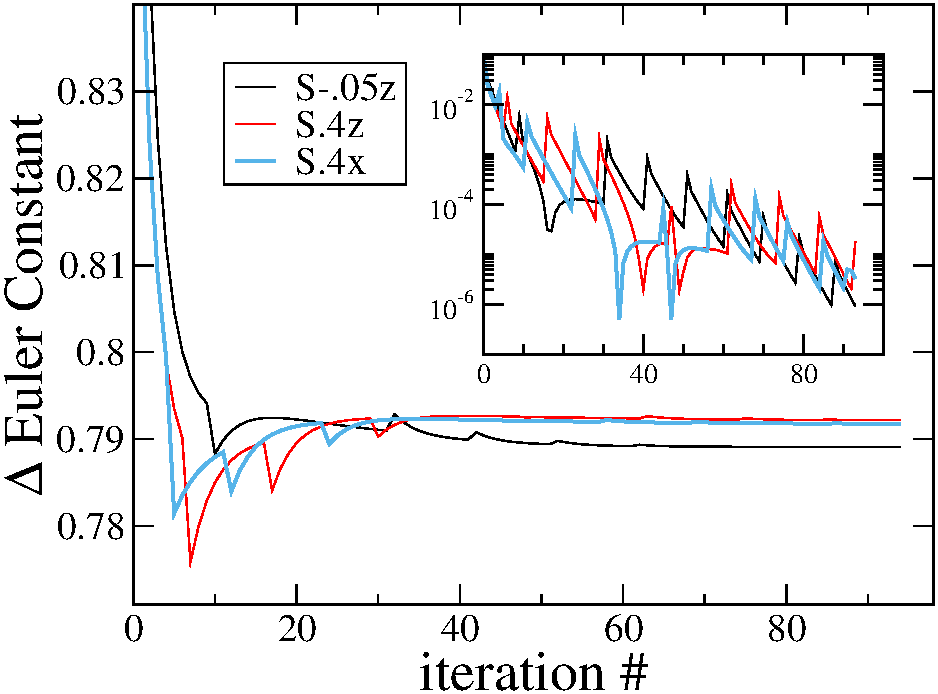
\includegraphics[width=0.95\columnwidth]{chap2/EulerConstConvergence}
\caption[Iterative convergence of the Euler constant.]{\label{fig:EulerConstConvergence}
Convergence of the Euler
  constant during iteration at the lowest resolution R0. The inset shows the difference
  between values at subsequent iterations.}
\end{figure}

\subsection{Convergence of the Solution}

Having established that our iterative procedure converges as intended,
we now turn out attention to the convergence of the solution with
resolution. 
To demonstrate it, we will look at the Hamiltonian and
momentum constraints, and the differences between measured physical
quantities - the ADM energy and ADM angular momentum, and the surface
fitting coefficients of the stars. As our initial data representation
is fully spectral, we expect that these quantities should converge
exponentially with resolution. Note that when we discuss the value of
a quantity at a certain resolution, we are referring to the value of
that quantity after the final iterative step at that
resolution. 

Figure~\ref{fig:HamMom} shows the convergence of the Hamiltonian
constraint and the Momentum constraint for our three runs of
interest. These are computed during the last iterative solve at each
resolution. The data plotted are computed as
\begin{equation}
H = ||\frac{R_\Psi}{8\Psi^5}||,
\end{equation}
\begin{equation}
M = ||\frac{R_{\beta}}{2\alpha\Psi^4}||.
\end{equation}
Here $R_\Psi$ and $R_\beta$ denote the residuals of Eqs.~(\ref{eq:XCTS-ConformalFactor}) and~(\ref{eq:XCTS-Shift}), respectively, and $||\,.\,||$ represents the root-mean-square value over grid-points of
the
 entire computational grid. 
This plot demonstrates that our initial
data solver converges  exponentially with resolution, even for
very high spins, which gives confidence that we are indeed correctly
solving the Einstein Field Equations.

\begin{figure}
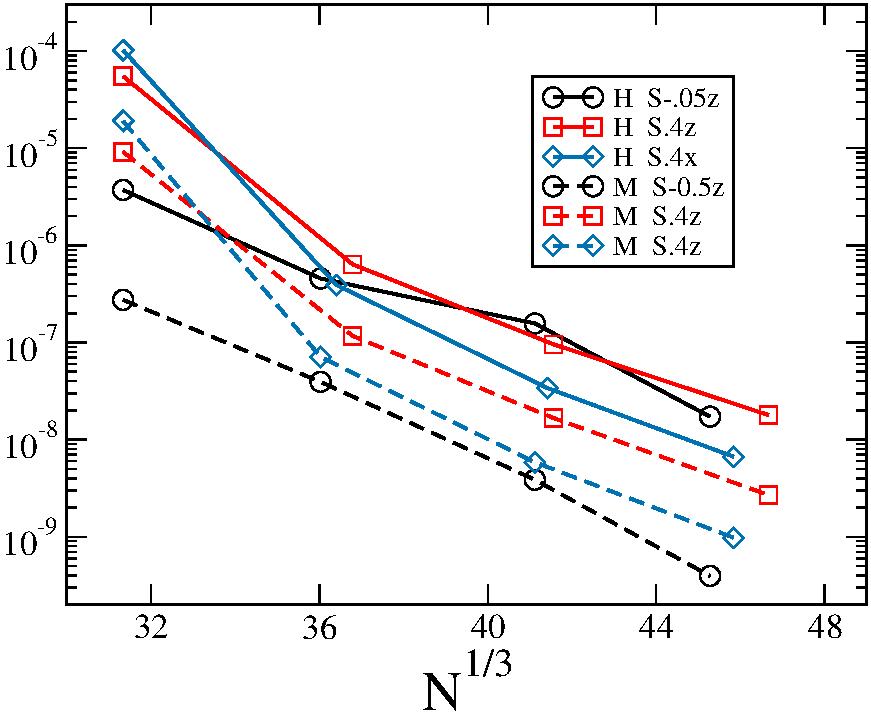
\includegraphics[width=0.95\columnwidth]{chap2/HamMom}
\caption[Convergence of the Hamiltonian and Momentum constraints.]{{\label{fig:HamMom}}Hamiltonian and Momentum constraints as a function of resolution $N$. We see exponential
  convergence in all cases.}
\end{figure}

 The surface of the star is represented by a spherical harmonic expansion:
\begin{equation}
R_s(\theta,\phi) = \sum^{l_{\rm max},m_{\rm
    max}}_{l,m}c_{lm}Y_{lm}(\theta,\phi),
\end{equation}
where $l_{\rm max}= m_{\rm max} = 11$, unless stated otherwise.
The stellar surface is located by finding a constant specific enthalpy surface, cf. Sec.~\ref{sec:IDalgorithm}, and the spherical subdomains that cover the star are deformed to conform to $R_s(\theta,\phi)$.
To establish convergence of the position of the stellar surface we
introduce the quantity
\begin{equation}
\label{eq:Deltac}
\Delta c(i) = \frac{1}{l(l+1)} \sqrt{\sum^{l_{\rm max},m_{\rm
      max}}_{l,m}\left(c_{lm}(i)-c_{lm}(N)\right)^2}.
\end{equation}
Here $i$ refers to the $i^{\rm th}$ resolution in the initial data,
and $N$ refers to the final resolution. Figure~\ref{fig:ClmDif} plots $\Delta c(i)$ vs. resolution. The surface location converges exponentially to better than $10^{-8}$.

\begin{figure}
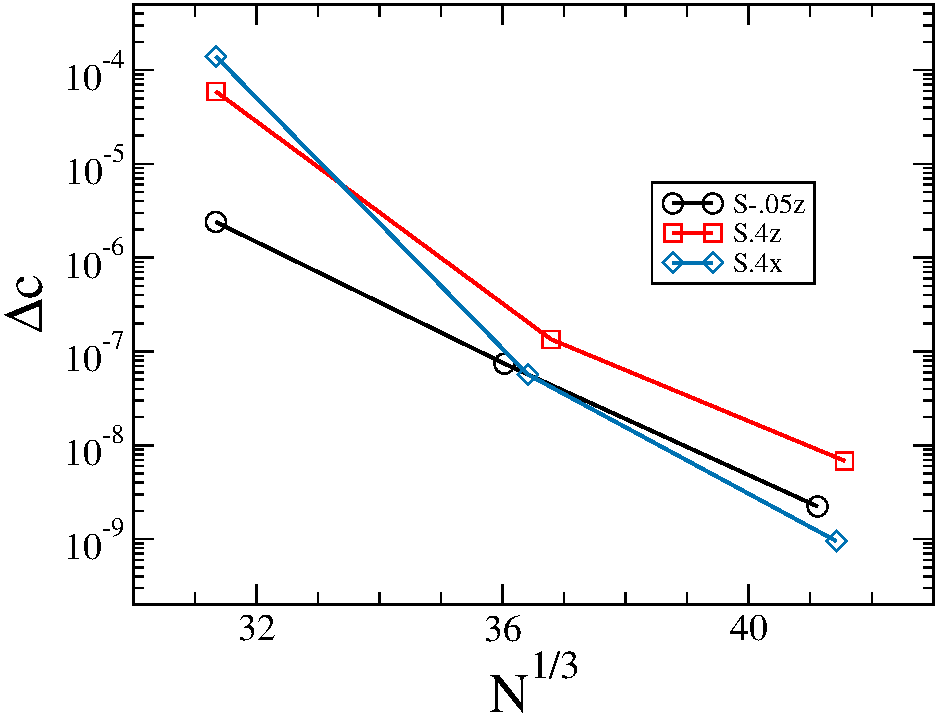
\includegraphics[width=0.95\columnwidth]{chap2/ClmDif}
\caption[Convergence of the location of the stellar surface.]{{\label{fig:ClmDif} Convergence of the location of the stellar surface}.
  Plotted is $\Delta c$ as defined in Eq.(~\ref{eq:Deltac}), for three representative configurations.}
\end{figure}

Finally, we assess the overall convergence of the solution through
the global quantities $E_{\rm ADM}$ and $\left|J^i_{\rm ADM}\right|$.
The surface integrals at infinity in these two quantities are recast using Gauss' law (cf.~\citep{FoucartEtAl:2008}):
\begin{align}
E_{\rm ADM} &= -\frac{1}{2\pi}\oint_{S_{\infty}}\delta^i_j\partial_i\Psi\, dS_j\nonumber \\
&= -\frac{1}{2\pi}\oint_{S}\delta^i_j \partial_i\Psi\, dS^j  +\frac{1}{2\pi}\int_{\mathcal{V}}\delta^{ij}\partial_i\partial_j\Psi\,dV,
\end{align}
and
\begin{align}
J^{z}_{\rm ADM} 
& = \frac{1}{8\pi}\oint_{S_{\infty}}\left(xK^{yj}-y K^{xj}\right)dS_j\nonumber\\
& = \frac{1}{8\pi}\oint_{S}\left(xK_{yi}-yK_{xi}\right)\delta^{ij}\Psi^2\,dS_j.
\end{align}
Here $\mathcal V$ is the volume outside $S$, and the integrals are evaluated in the flat conformal space. To obtain the other components of $J_{\rm ADM}^i$, cyclically permute the indices x,y,z.
 We define the quantities $\Delta E$ and $\Delta J$ as the absolute fractional difference in these quantities between the current resolution and the next highest resolution. These are plotted in figure~\ref{fig:EADMConvergence}.  
In general, we find
agreement at the $10^{-7}-10^{-8}$ level by the final
resolution.

\begin{figure}
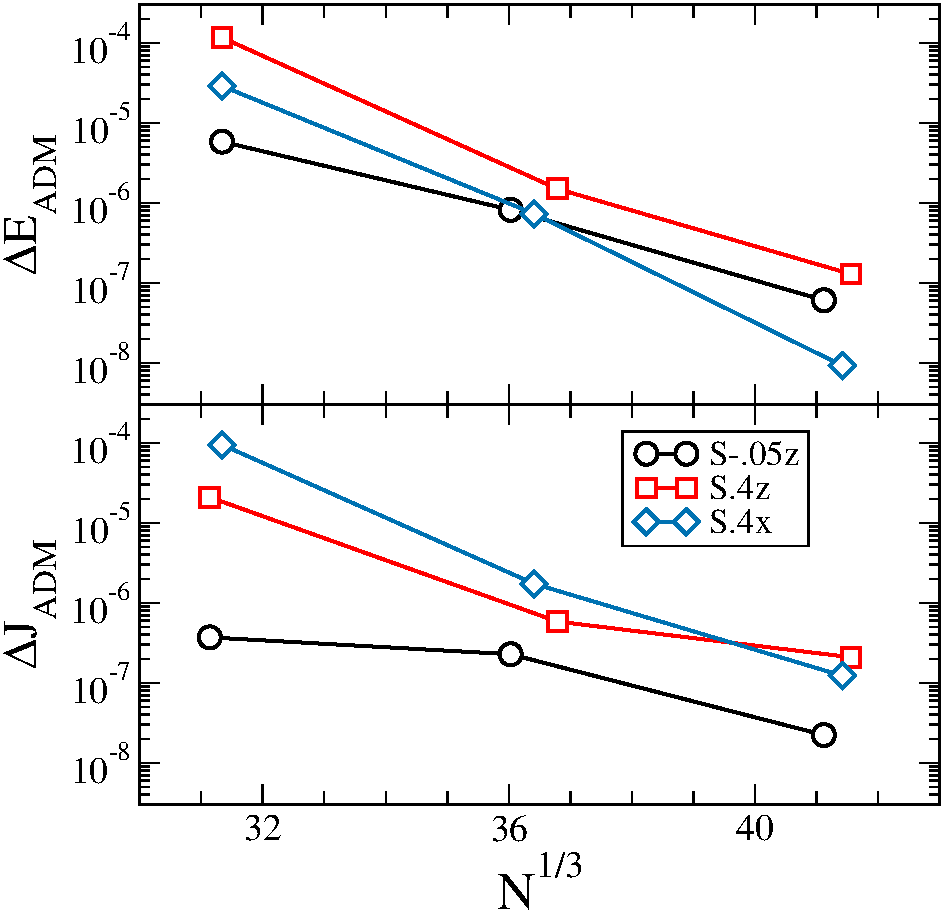
\includegraphics[width=0.95\columnwidth]{chap2/EADMConvergence}
\caption[Convergence of ADM-energy and of the ADM-angular momentum magnitude.]{{\label{fig:EADMConvergence}} Convergence of ADM-energy and the magnitude of the ADM-angular momentum. Shown are the fractional differences between neighboring resolutions, as a function of the lower resolution.
}
\end{figure}




















\subsection{Convergence of the Quasilocal Spin}

\begin{figure}
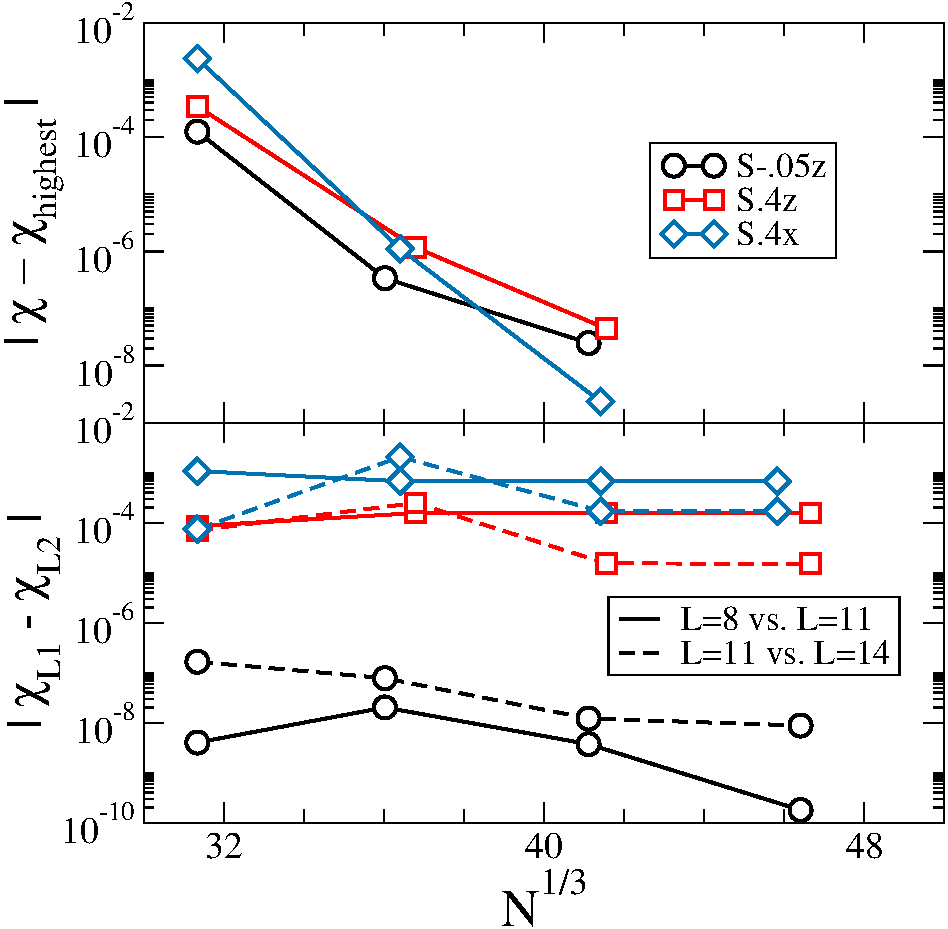
\includegraphics[width=0.95\columnwidth]{chap2/SpinConvergence}\\


\caption[Convergence of the quasilocal spin computation.]{\label{fig:SpinConvergence} Convergence of the quasilocal
  spin computation. {\bf Top panel:} difference of spin computed at
  resolution $N$ with the spin computed at the highest resolution.
  {\bf Bottom panel:} Difference between spins computed at different
  resolution $L$ of the spin-computation. For {\tt S-.5z}, we achieve an
  accuracy of $\sim 10^{-7}$, whereas for {\tt S.4z} and {\tt S.4x}, the accuracy
  is $\sim 10^{-4}$ due to finite $L$.}
\end{figure}

We now turn to the angular momentum of the neutron stars, as measured
with quasilocal angular momentum integrals on the stellar surface.
We will discuss dimensionless spins $\chi$, which depend on two
distinct numerical resolutions: First, the resolution of the
3-dimensional grid used for solving the initial value equations. This
resolution is specified in terms of $N$, the total number of
grid-points. Second, the resolution used when solving the eigenvalue
problem for approximate Killing vectors on the 2-dimensional surface,
as given by $L$, the expansion order in spherical harmonics of
  the surface-parameterization
  $r_S(\theta,\phi)=\sum_{l=0}^L\sum_m r_{lm}Y^{lm}(\theta,\phi)$.

Throughout this chapter, we use $L=11$. The top panel of
Fig.~\ref{fig:SpinConvergence} shows convergence of $\chi$ with
grid-resolution $N$, at fixed $L=11$. We find near exponential
convergence.

The influence of our choice $L=11$ is examined in the lower panel by
computing the quasilocal spin at lower resolution $L=8$ and at higher
resolution $L=14$. Changing $L$ impacts $\chi$ by $\sim 10^{-8}$ for
the low-spin case {\tt S-.05z}, and by $\sim 10^{-4}$ for the high-spin
cases {\tt S.4z} and {\tt S.4x}. For the high-spin cases, the spin
  measurement is convergent with increasing $L$, and the finite value
  of $L$ dominates the error budget. For the low-spin case, numerical
  truncation error dominates the error budget and convergence with $L$
  is not visible. High NS spin leads to a more distorted stellar
  surface, and so a fixed $L=11$ yields a spin result of lower
  accuracy. However, in all cases the the numerical errors of our
  spin measurements are still neglible for our purposes.

\begin{figure}
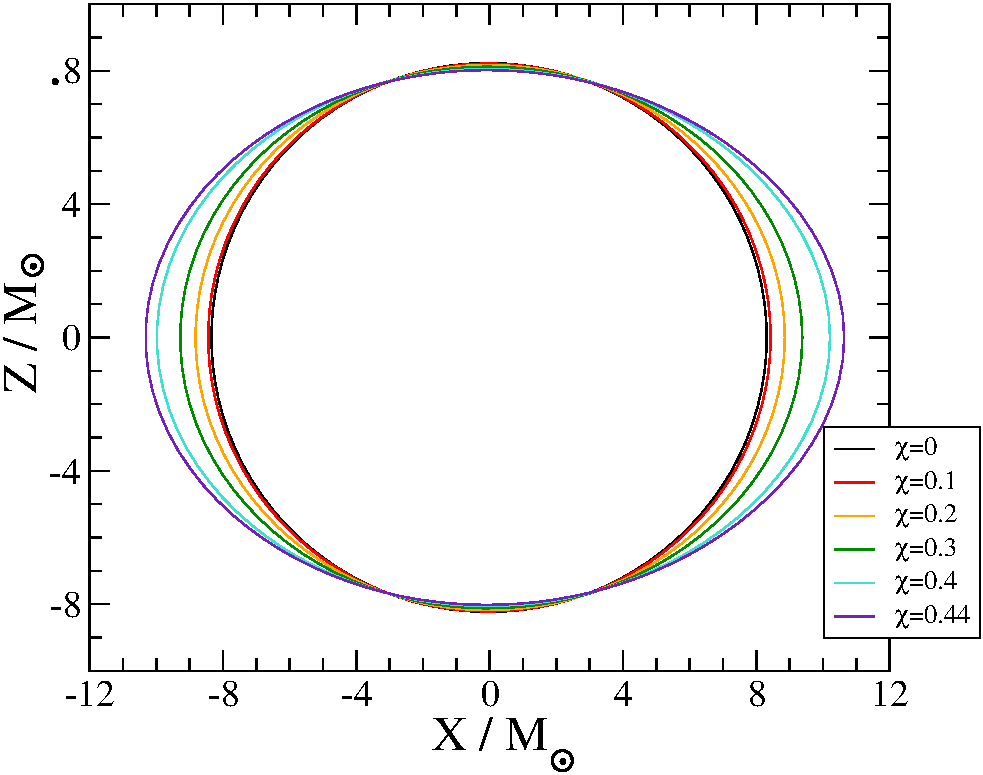
\includegraphics[width=0.98\columnwidth]{chap2/Bulging}
\caption[Stellar cross-section for a series of different spins.]{{\label{fig:Bulging}}Stellar cross-sections in the X-Z plane for a
  series of different spins, aligned with the $\hat{z}$ axis,
  demonstrating that they bulge at the equator in the expected way
  with increasing spin.}
\end{figure}


%%%%%%%%%%%%%%%%%%%%%%%%%%%%%%%%%%%%%%%%%%%%%%%%%%%%%%%%%%%%%%%%
\subsection{Quasilocal Spin}
\label{sec:QLSpinProperties}
%%%%%%%%%%%%%%%%%%%%%%%%%%%%%%%%%%%%%%%%%%%%%%%%%%%%%%%%%%%%%%%%

As discussed in section~\ref{sec:QLSpinExplanation}, we use a
quasilocal spin to define the angular momentum carried by each
neutron star. To our knowledge, this is the first application of this
method to neutron stars in binaries. 

In this section, we explore properties of the rotating BNS initial
datasets and the employed quasilocal spin diagnostic.


To explore the spin-dependence of BNS initial data sets, we
construct a sequence of equal-mass, equal-spin BNS binaries, with
spins parallel to the orbital angular momentum. We fix the initial
data parameters $M^b_{\rm NS}$, $D_0$, $\Omega_0$ and $\dot{a}_0$ to
their values for a configuration that we will also evolve below (specifically,  {\tt S.4z} - Ecc1)


\begin{figure}
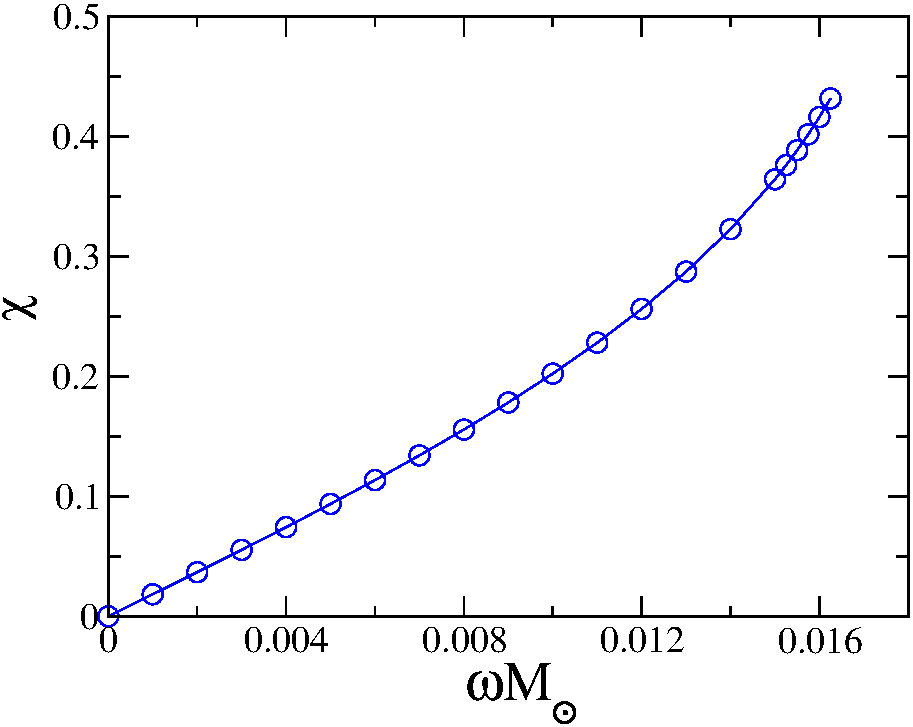
\includegraphics[width=0.95\columnwidth]{chap2/ChiVOmega}
\caption[Dimensionless angular momentum as a function of $\Omega$.]{{\label{fig:ChiVOmega}}Dimensionless angular momentum $\chi$ as a function of $\Omega$ for
  a series of spin-aligned initial data sets with the same physical
  parameters as our runs of interest. We see, as expected, a linear
  relation between $\chi$ and $\Omega$ at low-spins, which eventually
  becomes non-linear at higher spins. }
\end{figure}


Figure~\ref{fig:Bulging} shows cross-sections through one of the neutron stars
in the xz-plane, i.e. a plane orthogonal to the orbital plane which is
intersecting the centers of both stars. With increasing spin, the
stars develop an increasing equatorial bulge, an expected consequence of centrifugal forces. 

Figure~\ref{fig:ChiVOmega}
presents the dimensionless spin of either neutron star as a function
of $\omega$. $\chi$ increases monotonically with the rotation
parameter $\omega$. 
The spin $\chi$ increases
linearly with $\omega$ for small $\omega$. For larger $\omega$, the
dependence steepens, as the increasing equatorial radius of the stars
increase the moment of inertia~\citep{Worley:2008cb}. 

For
$\omega=0.01625 M_{\odot}^{-1}$ we achieve $\chi=0.432$, the largest spin we are
able to construct. This is reasonably close to the theoretical
maximum value for $\Gamma=2$ polytropes,
$\chi\sim 0.57$~\citep{Ansorg:2003br}. Above $\omega=0.01625 M_{\odot}^{-1}$,
the initial data code fails to converge. The steepening of the $\chi$
vs. $\omega$ curve is reminiscent of features related to
non-uniqueness of solutions of the extended conformal thin sandwich
equations~\citep{Lovelace2008,Pfeiffer-York:2005,Baumgarte2007,Walsh2007},
and it is possible that our failure to find solutions originates in an analogous
break-down of the uniqueness of solutions of the constraint equations.


While the focus of our investigation lies on rotating NS, we
  note that for $\omega=0$ our data-sets reduce to the standard
  formalism for irrotational NS. For $\omega=0$, we find a
  quasilocal spin of the neutron stars is $\chi=2\times 10^{-4}$.
  This is the first rigorous measurement of the residual spin of
  irrotational BNS. Residual spin is, for instance, important for the
  construction and validation of waveform models for compact object
  binaries. The analysis in~\cite{Boyle2007} indicates that
  spins of order $10^{-4}$ lead to a dephasing of about 0.01radians
  during the last dozen of inspiral orbits. This value is
  significantly smaller than the phase accuracy obtained by current
  BNS simulations, and so the residual spin is presently not a
  limiting factor for studies like~\citep{Bernuzzi:2014owa,Baiotti2011,Baiotti:2010xh}.

Finally, we demonstrate that the surface on which we
compute the quasilocal spin, does not significantly impact the spin
we measure: We choose coordinate spheres centered on the neutron star
with radius $R$, and compute the quasilocal spin using these
surfaces,
rather than the stellar surface.

In Fig.~\ref{fig:ChiVR}, we plot the spin measured on various $R=\rm{const}$
surfaces, for three different values of $\omega$, from the same sequences
shown in Fig.~\ref{fig:ChiVOmega}.

The circles denote spins extracted on coordinate spheres. The asterisks
indicate the spins computed on the stellar surface. The asterisk is
plotted at $R=R_{\rm eq}$, the equatorial radius of the neutron star
under consideration. 
We find good agreement between spins extracted on coordinate spheres and
the spin extracted on the stellar surface, as long as $R\ge R_{\rm eq}$. 
 The maximum disagreement is seen in the high spin curve, where
the two spins differ by $\sim 10^{-2}$. 

For $R<R_{\rm eq}$, the coordinate extraction sphere intersects the
outer layers of the neutron star and no longer encompasses the entire matter and angular
momentum of the star. Therefore, $\chi(R)$ shows a pronounced decline
for $R<R_{\rm eq}$ for each of the three initial-data sets considered
in Fig.~\ref{fig:ChiVR}. For $R>R_{\rm eq}$, $\chi(R)$ continues to
increase slightly, for instance, for the middle curve,
$\chi(R=9)=0.202$ whereas $\chi(R=11)=0.204$.

In summary, Fig.~\ref{fig:ChiVR} shows that the quasilocal spin
extracted on coordinate spheres can serve as a good approximation of
the quasilocal spin extracted on the stellar surface (as long as the
coordiate sphere is outside the star, of course).

This is important because during evolutions of the
binary, we do not track the surface of the star.
Instead, we will compute the spin on coordinate spheres, similarly to Fig.~\ref{fig:ChiVR}.

\begin{figure}
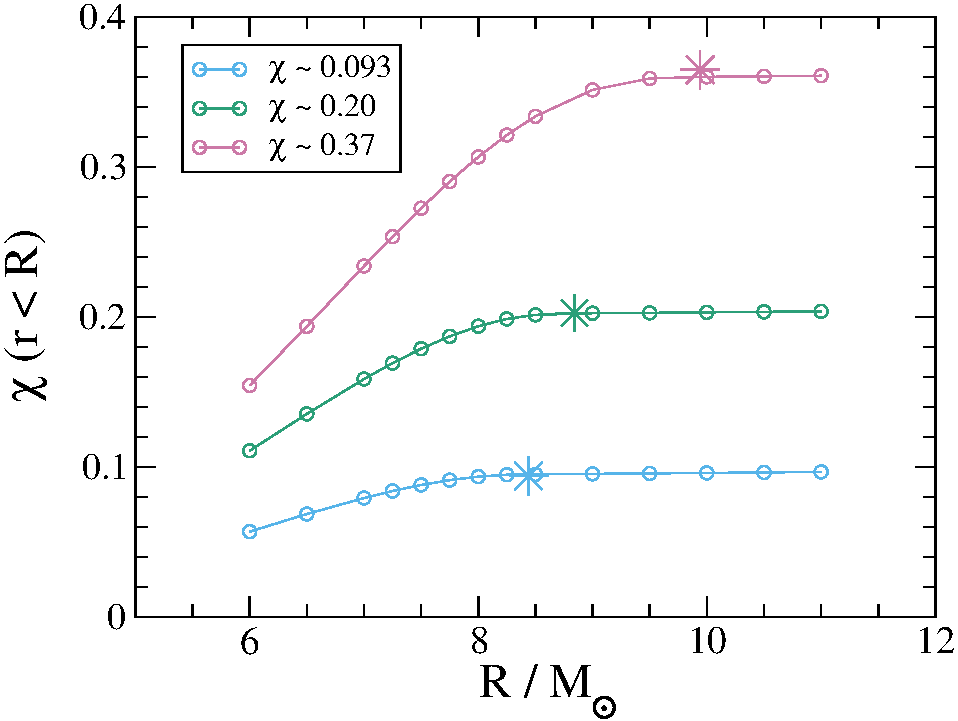
\includegraphics[width=0.95\columnwidth]{chap2/ChiVR}
\caption[Dimensionless spin measured as measured on different coordinate spheres.]{{\label{fig:ChiVR}}Dimensionless spin $\chi$ measured on
  coordinate spheres with radius $R$ for three different aligned spin
  BNS systems. The asterik denotes the spin measured on the
  (non-spherical) stellar surface. Circles to the right of the
  asterik represent coordinate spheres entirely outside the neutron
  star, and circles on the left of the asterik indicate spin
  measurement surfaces that intersect the star or are entirely located
  inside the star.}
\end{figure}



\section{Evolution Results}
\label{sec:EvolutionResults}

We now evolve the three configurations discussed in Sec.~\ref{sec:ID}.
As indicated in Table~\ref{tab:InitialData}, all three configurations
are equal-mass binaries, with individual ADM masses $M_\star$ (in
isolation) 
of $1.64M_{\odot}$ or $1.648M_{\odot}$ at initial separation of
$D=47.2M_\odot$, and using a polytropic equation of state with
$\Gamma=2.0$ and $\kappa=123.6$. Both stars have equal spins, and the
three configurations differ in spin magnitude and spin direction.
Configuration {\tt S-0.05z} has spin-magnitudes $\sim 0.05$ anti-aligned
with the orbital angular momentum, and the confiurations {\tt S.4z} and {\tt S.4x}
have spin magnitudes near 0.4, along the z-axis and x-axis,
respectively.

Each configuration is evolved through $\gtrsim 10$ orbits, into the
late-inspiral. In this chapter we focus on the inspiral of the neutron
stars. Table~\ref{tab:RunInfo} summarizes parameters for these runs.
\begin{table}
\centering
\begin{tabular} {c | c | c | c | c | c | c}
Name & $k$ & $e$ & $\vec{\chi}$ & $f_{0}(Hz)$ & $N_{\rm orb}$ & $t_{f}({\rm ms})$ \\ \hline
{\tt S.4z} & 0,1,2 & $\lesssim 0.001$ & $0.381\hat{z}$ & $167.7$ & $11.8$ & $56.0$ \\ \hline
{\tt S-.05z} & 0,1,2 & $0.0006$ & $-0.050\hat{z}$ & $165.4$ & $12.5$ & $56.3$ \\ \hline
{\tt S.4x} & 0,1 & $\lesssim 0.002$ & $0.375\hat{x}$ & $164.8$ & $9.1$ & $45.7$ \\ \hline
\end{tabular}
\caption[Detailed information about our three evolutions.]{ {\label{tab:RunInfo}} Information about our three evolutions. $k$ indicates the numerical resolutions on which a simulation is performed, $e$ indicates the smallest achieved orbital eccentricity. $\vec\chi$ and $f_0$ are the dimensionless spins at $t=0$ and the initial orbital frequency. Finally, $N_{\rm orb}$ and $t_f$ represent the number of orbits the configuration was evolved for, and the evolution time.}
\end{table}



\subsection{Evolution Code}
\label{sec:EvolutionCode}

In our evolution code, SpEC~\citep{Buchman:2012dw,Lovelace:2011nu,
  Scheel2009,Kidder2000a,Lindblom2006,Scheel2006,Szilagyi:2009qz,Lovelace:2010ne,
  Hemberger:2012jz,Ossokine:2013zga}, we use a mixed spectral --
finite-difference approach to solving the Einstein Field Equations
coupled to general relativistic hydrodynamics equations. The
equations for the space-time metric, $g_{\mu\nu}$ are solved on a
spectral grid, while the fluid equations are solved on a finite
difference grid, using a high-resolution shock-capturing scheme. We
use a WENO~\citep{Jiang1996202,Liu1994200} reconstruction method to
reconstruct primitive variables, and a Harten-Lax-van Leer (HLL) Riemann solver~\cite{HLL}
to compute numerical fluxes at interfaces. Integration is done using a
3rd order Runge-Kutta method with an adaptive stepsize. We interpolate
between the hydro and spectral grids at the end of each full time
step, interpolating in time to provide data during the Runge-Kutta
substeps
(see~\cite{Duez:2008rb,FoucartEtAl:2011,Foucart:2013a,Muhlberger2014}
for a more detailed description of the method). 

Each star is contained in a separate cubical finite
difference grid that does not overlap with that
of the other star. The sides of the grids are initially $1.25$ times
the stars' diameters. We use grids that contain $97^3$, $123^3$ and
$155^3$ points for resolutions $k=0,1,2$, respectively\footnote{For
  aligned-spin configurations {\tt S-.05z} and {\tt S.4z}, we take advantage of,
  and enforce, z-symmetry, which halves the number of grid-points
  along the z-axis.}. These resolutions correspond to linear
grid-spacing of $340\,\text{m}$, $268\,\text{m}$ and $213\,\text{m}$
respectively for the {\tt S.4z} case. The precessing evolution {\tt S.4x} uses
similar grid-spacing, whereas the anti-aligned run {\tt S-.05z} has a
slightly smaller grid-spacing because the stars themselves are
smaller. The region outside the NS but inside the finite
difference grid is filled with a low density
atmosphere with $\rho=10^{-13}M_{\odot}^{-2}$. The motion of the NSs
is monitored by computing the centroids of the NS mass distributions
\begin{equation}
\label{eq:centroid}
X^i_{\rm CM} = \int{x^iu^0\rho_0\sqrt{-g^{(4)}}d^3x}
\end{equation}
for each of the grid patches containing a NS.

The grids are rotated and their separation rescaled to keep the
centers of the NS at constant grid-coordinates~\citep{Scheel2006,Hemberger:2012jz,Scheel2014}. As the physical separation between the stars decreases, the rescaling of
grid-coordinates therefore causes the size of the stars to increase
in grid-coordinates. In order to avoid the stellar surfaces expanding
beyond the geometric size of the finite difference grid, we monitor the matter flux leaving
this grid along the x, y, and z-direction. If the matter flux is too
large along a certain axis, we expand the grid in that
direction. 
This procedure allows us to
dynamically choose the optimal grid-size that limits matter loss to a
small, user-specified level. When changing the size of the hydro
grid, the number of grid-points is kept constant, so this process
changes the effective resolution during the evolution.

The Einstein field equations are solved on a spectral grid using basis-functions appropriate for the shape of each subdomain.
For rectangular blocks, Cheybyshev polynomials are used along each axis; for a spherical shell (i.e. where the center is excised), spherical harmonics in angles, and Chebyshev polynomial in radius are employed; and for an open cylinder (i.e. with the region near the axis excised), Chebyshev polynomials and a Fourier series. For full spheres and filled cylinders, multi-dimensional basis-functions respecting the continuity conditions at the orign/axis are employed~\citep{Matsushima-Marcus:1995,1997JCoPh.136..100V}. For more details see~\cite{Muhlberger2014}. 


More specifically, our spectral
grid, the central region of each star is covered by a filled sphere
located at the center of the star. These have spherical harmonic modes
up to $L = 12+2k$. The radial basis-functions are one-sided Jacobi
polynomials with $7+k$ collocation points. The filled spheres are
surrounded by eight other spherical shells with the same radial and
angular resolutions. At the start of the evolution, the stellar
surface is generally located inside the third shell. The far field
region is covered by 20 spherical shells starting at 1.5 times the
inital binary separation and going out to 40 times that
separation. These shells have angular resolution $L=9+2k$ and radial
resolution $6+k$. The region between the innermost shell and the
stars is covered by a set of cylindrical shells and filled cylinders.

We use a generalized harmonic evolution system~\citep{Pretorius2006,Pretorius2005a,Lindblom2006} with 
 coordinates $x^{\mu}$ such that they satisfy a
wave equation
\begin{equation}
\nabla^{\nu}\nabla_{\nu}x^{\mu} = H^{\mu},
\end{equation}
for some freely-specifiable source function $H^{\mu}$. The initial
source function $H^\mu_{\rm initial}$ is determined by the intial
data, assuming that the time derivatives of the lapse and
shift functions initially vanish in the corotating frame. 
We then transition to a pure harmonic gauge, $H^{\mu}=0$ by
using a transition function, i.e.
\begin{equation}
H^\mu = e^{-\left(t/\tau\right)^4}\; H^\mu_{\rm initial}.
\end{equation}
The timescale $\tau$ is determined by $\tau=2\sqrt{d^3/(2M_\star)}$.
This is slow enough to avoid numerical gauge artifacts in the simulations.

%%%%%%%%%%%%%%%%%%%%%%%%%%%%%%%%%%%%%%%%%%%%%%%%%%%%%%%%%%%%%%%%
\subsection{Eccentricity Removal}
\label{sec:EccRemoval}
%%%%%%%%%%%%%%%%%%%%%%%%%%%%%%%%%%%%%%%%%%%%%%%%%%%%%%%%%%%%%%%%

Gravitational wave emission reduces orbital eccentricity rapidly during
a GW-driven inspiral~\citep{PetersMathews1963,Peters1964}. Therefore
inspiraling binary neutron stars are expected to have essentially
vanishing orbital eccentricity in their late inspiral, unless they recently
underwent dynamical interactions. Our goal is to model
non-eccentric inspirals. In this subsection we demonstrate that we can
indeed control and reduce orbital eccentricty, using the techniques
developed for developed for black hole - black hole
binaries~\citep{,Pfeiffer-Brown-etal:2007,Boyle2007,Buonanno:2010yk}
and also applied to black hole - neutron star binaries~\citep{FoucartEtAl:2008}.


\begin{figure}
  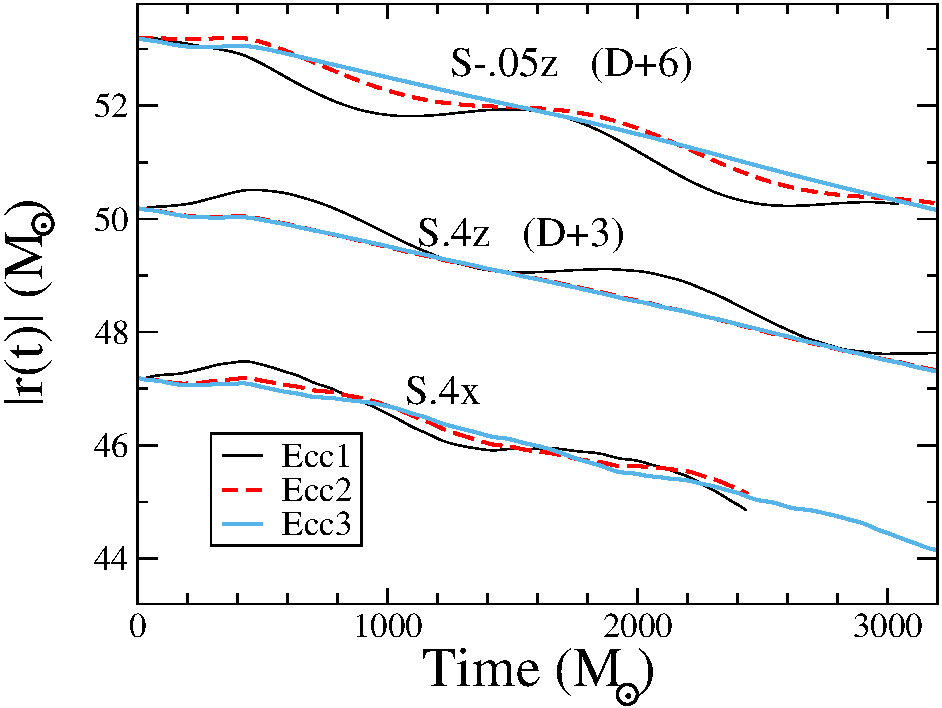
\includegraphics[width=0.95\columnwidth]{chap2/DvT2}\caption[Binary separation as a function of time.]{
{\label{fig:DvT}}
The
    binary separation as a function of time. Shown are three
    eccentricity removal iterations (Ecc1,Ecc2,Ecc3) for each of the
    three configurations studied. The data for {\tt S-.05z} and {\tt S.4z} is
    offset vertically by 6 and 3, respectively, for clarity of
    plotting.}
\end{figure}


For fixed binary parameters (masses, spins), and fixed initial
separation $D_0$, the initial orbit of the binary is determined by two
remaining parameters: The initial orbital frequency $\Omega_0$, and
the initial radial velocity, which we describe through an expansion
parameter $\dot{a}_0 = \dot{r}/r$. These two parameters will encode
orbital eccentricty and phase of periastron, and our goal is to
determine these parameters to reduce orbital eccentricity. We
accomplish this using an iterative procedure first introduced
  for binary black holes~\citep{Boyle2007,Buonanno:2010yk}. An initial
data set is evolved for a few orbits, the resulting orbital dynamics
are analyzed, and then the initial data parameters $\Omega_0$ and
$\dot a_0$ are adjusted.


\begin{table}
\centering
\begin{tabular} {l | l | c | c}
Name & $\Omega\times10^{3}$ & $\dot{a}_0\times10^{5}$ & $e$
\\ \hline {\tt S.4z} - Ecc1 & $5.10538$ & $0$ & $0.006$ \\ {\tt S.4z} - Ecc2 &
$5.09591$ & $-1.60$ & $\lesssim 0.001$ \\ {\tt S.4z} - Ecc3 & $5.09594$ &
$-1.75$ & $\lesssim 0.001$ \\ \hline {\tt S-.05z} - Ecc1 & $5.10538$ & $0$ &
$0.008$ \\ {\tt S-.05z} - Ecc2 & $5.11561$ & $0$ & $0.004$ \\ {\tt S-.05z} - Ecc3
& $5.11769$ & $-1.71$ & $0.0006$ \\\hline {\tt S.4x} - Ecc1 & $5.10538$ &
$0$ & $0.007$ \\ {\tt S.4x} - Ecc2 & $5.10429$ & $-2.27$ & $0.004$ \\ {\tt S.4x} -
Ecc3 & $5.10064$ & $-2.36$ & $\lesssim 0.002$ \\
\end{tabular}
%\end{center}
\caption[Eccentricity removal data for our three main runs.]{\label{tab:ecc_removal} Eccentricity removal for the three
  main runs discussed in this chapter. Only initial orbital frequency
  $\Omega_0$ and initial radial expansion factor $\dot a_0$ are
  changed between different EccN iterations. Recall that these
  quantities have units of $M_{\odot}^{-1}$.}
\end{table}

%%%%%%%%%%%%%%%%%%%%%%%%%%%%%%%%%%%%%%%%%%%%%%%%%%%%%%%%%%%%%%%%
\begin{figure}
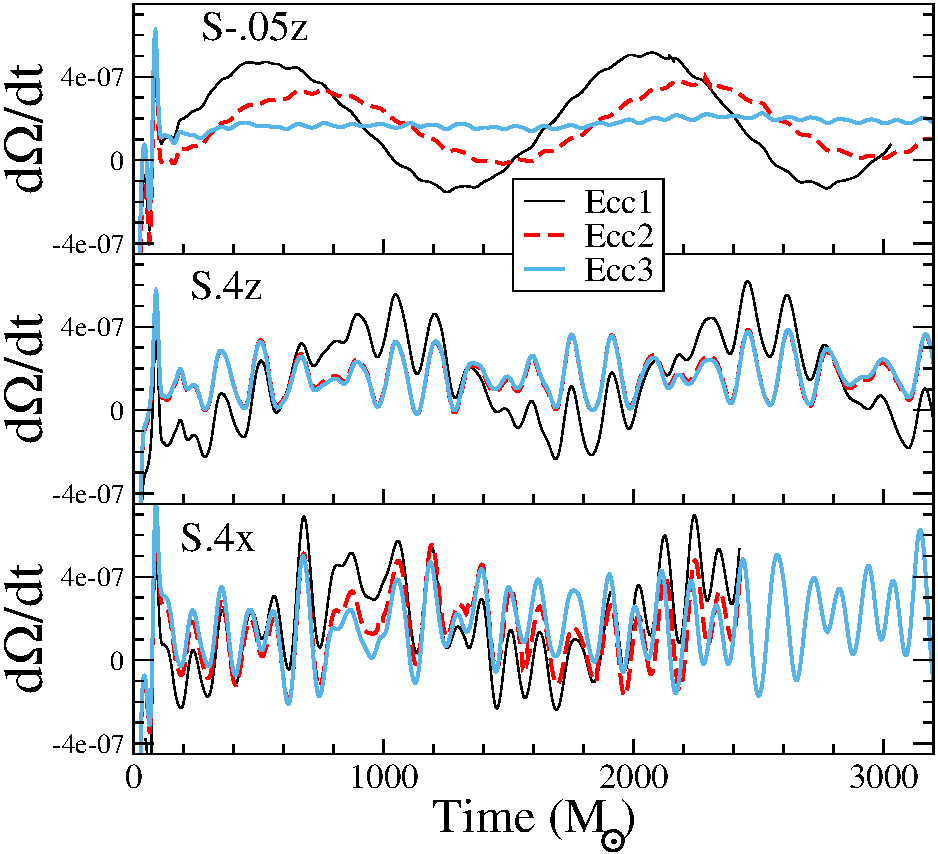
\includegraphics[width=0.95\columnwidth]{chap2/DOmegaVT}
\caption[The derivative of the binary orbital frequency at different levels of eccentricity reduction.]{{\label{fig:DOmegaVT}} The derivative of the binary orbital
  frequency as a function of time for different levels of
  eccentricity reduction for our three runs of interest. Note that
  $d\Omega/dt$ has units of $M_{\odot}^{-2}$. }
\end{figure}
%%%%%%%%%%%%%%%%%%%%%%%%%%%%%%%%%%%%%%%%%%%%%%%%%%%%%%%%%%%%%%%%


For binary neutron stars, we initialize the first iteration
of eccentricity removal, with $\dot{a}_0=0$ and use
$\Omega_0$ determined from irrotational BNS initial data, based on
the equilibrium condition in Eq.~\ref{eq:OmegaEq}. Evolutions with
these choices are labeled with the suffix ``Ecc1'', and show noticable
variations in the separation between the two NS, cf. the solid black
lines in Fig.~\ref{fig:DvT}.

We
compute the trajectories of the centers of mass of each star, as
  determined by Eq.~\ref{eq:centroid},
$\vec c_1(t)$ and $\vec c_2(t)$, and using the relative separation
$\vec r=\vec c_2(t) - \vec c_1(t)$, compute the orbital frequency
\begin{equation}
\label{eq:Omega}
\Omega(t) = \frac{|\vec r(t)\times\dot{\vec{r}}(t)|}{r(t)^2},
\end{equation}
where an over-dot indicates a numerical time-derivative.
Finally, we compute $\dot{\Omega}(t)$ and fit it to a function of the form
\begin{align}
\dot{\Omega}(t) = & A_1(t_c-t)^{-11/8} + A_2(t_c-t)^{-13/8}\nonumber \\
&+ B_0\cos{(B_1t
  + B_2t^2 + B_3)}.
\end{align}
The power law parts of this fit represent the orbital decay due to the
emission of gravitational waves, while the oscillatory part represents
the eccentric part of the orbit. We then update $\Omega_0$ and
$\dot{a}_0$ with the formulae (see \cite{Buonanno:2010yk} for a
detailed overview)
\begin{align}
  \Omega_0 \leftarrow \Omega_0 - \frac{B_0B_1}{4\Omega_0^2}\sin B_3, \\
  \dot{a}_0\leftarrow \dot{a}_0 +\frac{B_0}{2\Omega_0}\cos B_3.
\end{align}
We repeat this procedure twice, resulting in simulations with suffix
Ecc2 and Ecc3. Table~\ref{tab:ecc_removal} summarizes the orbital
parameters for the individual simulations, and Figs.~\ref{fig:DvT}
and~\ref{fig:DOmegaVT} illustrate the efficacy of the procedure
through plots of separation and time-derivative of orbital frequency.
The eccentricity is successfully reducued from $e\sim 1\%$ to
$\sim 0.1\%$. After two eccentricity reduction iterations, variations
in $\dot\Omega(t)$ are so small that they are no longer discernible
from higher-frequency oscillations in $\dot\Omega(t)$,
cf. Fig.~\ref{fig:DOmegaVT}.

%%%%%%%%%%%%%%%%%%%%%%%%%%%%%%%%%%%%%%%%%%%%%%%%%%%%%%%%%%%%%%%%
\begin{figure}
  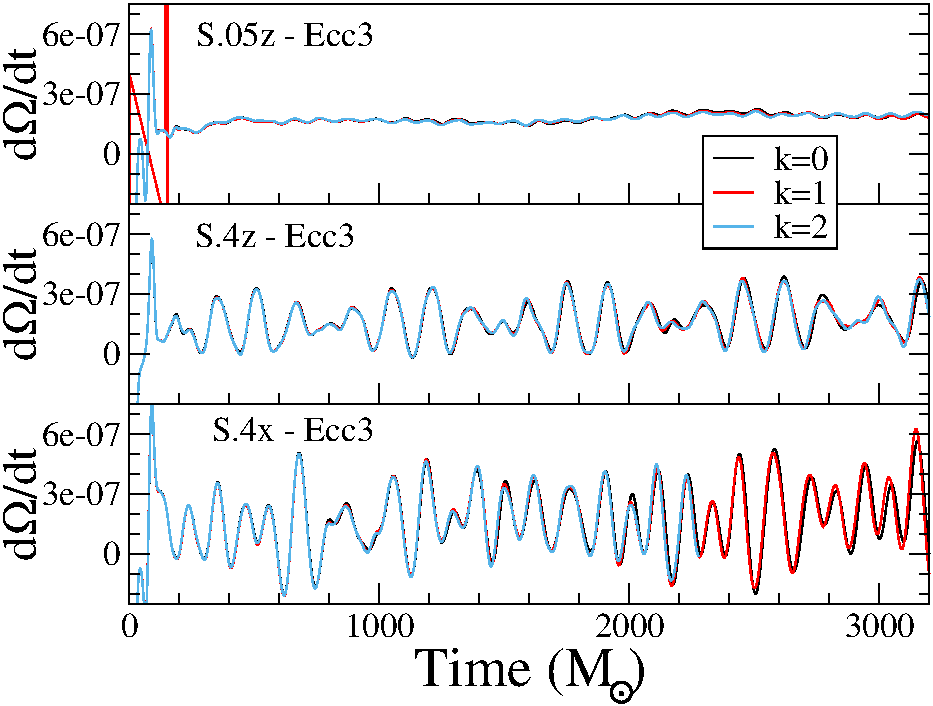
\includegraphics[width=0.92\columnwidth]{chap2/OmegaDotComparison}
  \caption[Convergence of the derivative of the binary orbital frequency.]{ {\label{fig:OmegaDotComparison}Convergence of
      $\dot\Omega(t)$. Shown are $\dot\Omega(t)$ at three different
      numerical resolutions ($k=0,1,2$) for the final,
      lowest-eccentricity initial data. The oscillations in
      $\dot\Omega(t)$ are evidently not caused by numerical truncation
      error. Note that $\dot{\Omega}$ has units of $M_{\odot}^{-2}$.}}
\end{figure}
%%%%%%%%%%%%%%%%%%%%%%%%%%%%%%%%%%%%%%%%%%%%%%%%%%%%%%%%%%%%%%%%

The high frequency oscillations in $\dot\Omega(t)$ are caused by the
quasi-normal ringing of the neutron stars, as discussed in detail
below in Sec.~\ref{sec:QNModes}. Here, we only note that these
oscillations are convergently resolved,
cf. Fig.~\ref{fig:OmegaDotComparison}, and are therefore a genuine
feature of our initial data. Figure~\ref{fig:OmegaDotComparison} also
confirms that the lowest resolution ($k=0$) gives adequate resolution
for eccentricity removal.

The eccentricity removal algorithm attempts to isolate variations on
the orbital time-scale as the signature of eccentricity. For
{\tt S.4z} - Ecc2, it reports $e=0.0005$ and for {\tt S.4z} - Ecc3, $e=0.0002$.
However, given the large amplitude of the quasi-normal mode ringing, we consider
these estimates unreliable, and therefore quote an upper bound of
0.001 in Table~\ref{tab:ecc_removal}. Similarly, for {\tt S.4x} - Ecc3, the fitting
reports $e=0.001$, and we quote a conservative upper bound of 0.002.

%%%%%%%%%%%%%%%%%%%%%%%%%%%%%%%%%%%%%%%%%%%%%%%%%%%%%%%%%%%%%%%%
\subsection{Aligned spin BNS Evolutions: NS Spin}
\label{sec:EvolutionSpin}
%%%%%%%%%%%%%%%%%%%%%%%%%%%%%%%%%%%%%%%%%%%%%%%%%%%%%%%%%%%%%%%%

In this section, we will discuss the measurement of spins during our
evolutions for the non-precessing cases, {\tt S.4z} and {\tt S-.05z}. Aligned
spin binaries do not precess. Combined with the low viscosity we
expect the NS spins to stay approximately constant during the
evolutions. These systems therefore serve as a test on our spin
diagnostics during the evolutions.
In this section, and through the rest of this chapter, we always use the
final eccentricity reduction, ``Ecc3''. For brevity, we will omit the
suffix ``-Ecc3'', and refer to the runs simply as {\tt S-.05z}, etc.

%%%%%%%%%%%%%%%%%%%%%%%%%%%%%%%%%%%%%%%%%%%%%%%%%%%%%%%%%%%%%%%%
\begin{figure}
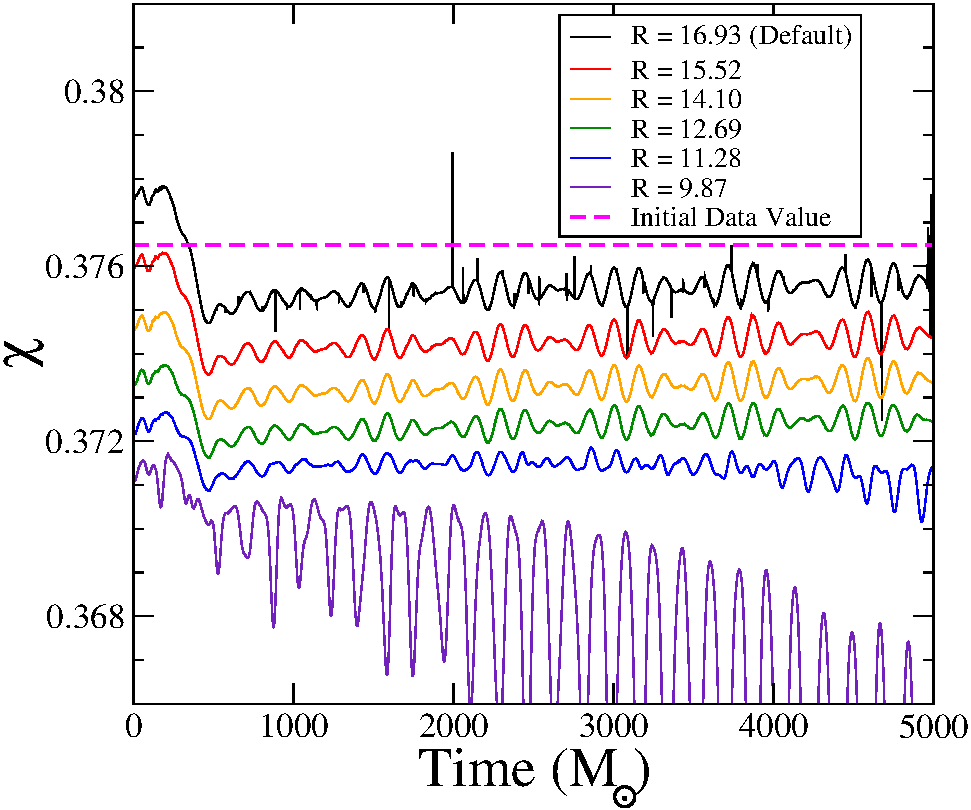
\includegraphics[width=0.95\columnwidth]{chap2/ChiVTZoomed}
\caption[The spin measured on multiple
  coordinate spheres for the {\tt S.4z} run.]{{\label{fig:ChiVTZoomed}} The spin measured on multiple
  coordinate spheres for the {\tt S.4z} run.}
\end{figure}
%%%%%%%%%%%%%%%%%%%%%%%%%%%%%%%%%%%%%%%%%%%%%%%%%%%%%%%%%%%%%%%%

We do not track the surface of the star during the evolution.
Instead we simply evaluate the quasilocal spin of the stars on
coordinate spheres in the frame comoving with the binary. We must
therefore verify that the spin measured is largely independent of the
radius of the sphere, and that it is maintained during the evolutions
at the value consistent with that in the initial data.
Figure~\ref{fig:ChiVR} established that coordinate spheres can be used
to extract the quasilocal spin in the initial data.
Figure~\ref{fig:ChiVTZoomed} shows the results for the high-spin
simulation {\tt S.4x} during the inspiral.

%%%%%%%%%%%%%%%%%%%%%%%%%%%%%%%%%%%%%%%%%%%%%%%%%%%%%%%%%%%%%%%%
\begin{figure}
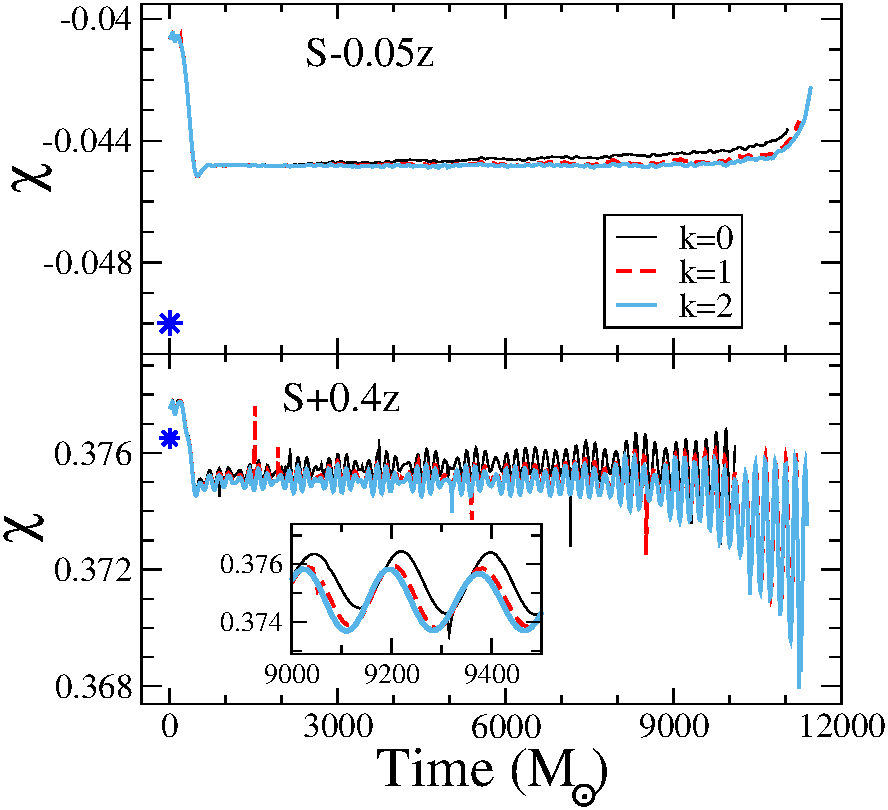
\includegraphics[width=0.99\columnwidth]{chap2/ChiVTDifferentRes2}
\caption[Neutron star spin during the two aligned-spin evolutions.]{{\label{fig:ChiVTDifferentRes2}} Neutron star spin during the
  two aligned-spin evolutions. Shown are three different numerical
  resolutions, $k=0$ (lowest), $k=1$, and $k=2$ (highest). The
  asterisk indicates the spin measured on the stellar surface in the
  initial data.}
\end{figure}
%%%%%%%%%%%%%%%%%%%%%%%%%%%%%%%%%%%%%%%%%%%%%%%%%%%%%%%%%%%%%%%%

For coordinate spheres with radii $R=11.28M_\odot$ to $R=16.93M_\odot$
in grid coordinates, the spins remain roughly constant in time. The
different extraction spheres yield spins that agree to about 1\%, with
a consistent trend that larger extraction spheres result in slightly
larger spins (as already observed in the initial data). The
horizontal dashed line in Fig.~\ref{fig:ChiVTZoomed} indicates the
spin measured on the stellar surface (i.e. not on a coordinate sphere)
in the initial data. We thus find very good agreement between all
spin measurements, and conclude that the quasilocal spin is reliable
to about 1\%.

The extraction sphere $R=9.87M_\odot$ in Fig.~\ref{fig:ChiVTZoomed}
intersects the outer layers of the neutron star. Because the
quasilocal spin captures only the angular momentum within the
extraction sphere, the value measured on $R=9.87M_\odot$ falls as our
comoving grid-coordinates cause this coordinate sphere to slowly move
deeper into the interior of the star. This behavior, again, is
consistent with Fig.~\ref{fig:ChiVR}.

These tests of using multiple coordinate spheres were only run for
about half of the inspiral -- enough to establish that the method is
robust. Subsequently, we report spins measured on the largest
coordinate sphere, $R=16.93M_\odot$.

The full behavior of the spin during the inspiral is shown in
figure~\ref{fig:ChiVTDifferentRes2} for both the {\tt S.4z} and {\tt S-.05z} runs.
Comparing the spin at different resolutions, we note that the data for
$k\!=\!1$ and $k\!=\!2$ are much closer to each other than compared to
$k\!=\!0$, indicating numerical convergence. We note that the impact
of numerical resolution (as shown in
Fig.~\ref{fig:ChiVTDifferentRes2}) is small compared to the
uncertainty inherent from the choice of extraction sphere,
cf. Fig.~\ref{fig:ChiVTZoomed}. We also note that for the first
$10000M_{\odot}$ of the run, the measured spin behaves as a constant,
as expected, albeit with some small oscillations. However,
afterward, we notice the
absolute value of the spin starts to decrease in both cases.
Finally, we note that in both cases, the spin measured in the inital
data on the stellar surface is within $\Delta \chi = 0.008$ of the spin
measured during the evolution. 

%%%%%%%%%%%%%%%%%%%%%%%%%%%%%%%%%%%%%%%%%%%%%%%%%%%%%%%%%%%%%%%%
\begin{figure}
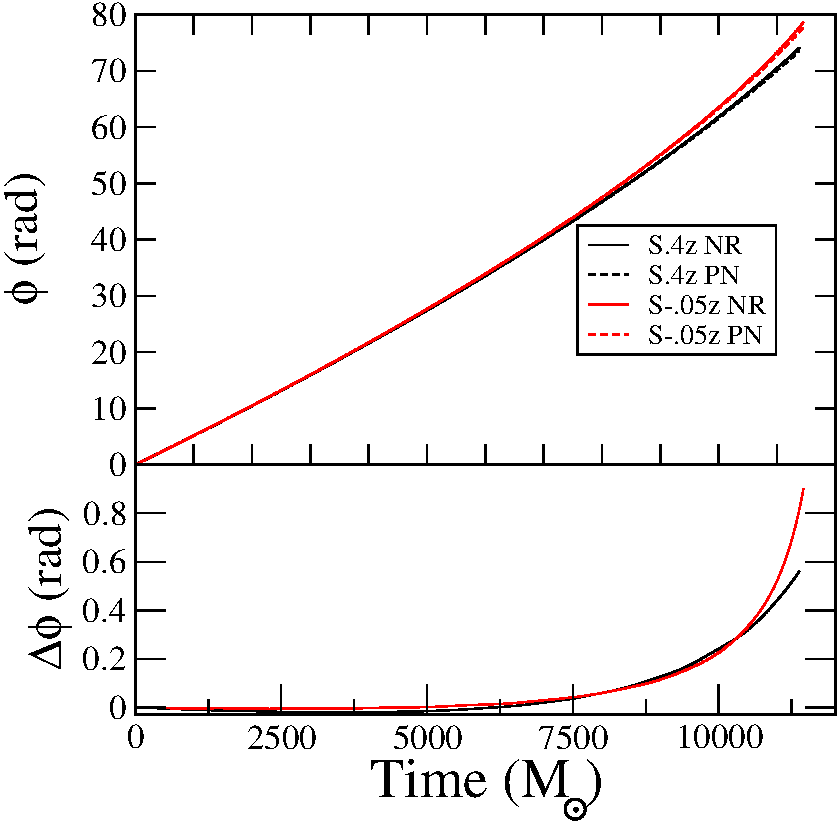
\includegraphics[width=0.95\columnwidth]{chap2/PhaseComparison}
\caption[Accumulated orbital phase as a function of time for our aligned and anti-aligned runs.]{ {\label{fig:Hangup}} Accumulated orbital phase as a function
  of time for our anti-aligned, {\tt S-.05z}, and aligned, {\tt S.4z}, runs. The
  dashed lines are Taylor T4 Post-Newtonian (PN) simulations simulations. The PN simulations were
  matched to NR in the intervals [1109,3956] and [2090,4904]
  respectively. Qualitatively, there
  is excellent agreement with the numerical data. The lower panel
  shows the difference
  $\Delta\phi(t)=\phi_{\rm NR}(t)-\phi_{\rm PN}(t)$.}
\end{figure}
%%%%%%%%%%%%%%%%%%%%%%%%%%%%%%%%%%%%%%%%%%%%%%%%%%%%%%%%%%%%%%%%

Finally, we compute the orbital phase 
\begin{equation}
\phi(t) = \int_0^t \Omega(t')\, dt',
\end{equation}

where the orbital frequency $\Omega(t)$ is given by
Eq.~(\ref{eq:Omega}).
The result is plotted in Fig.~\ref{fig:Hangup}, along with the

Post-Newtonian prediction for the same binary parameters (spins,
masses and initial orbital frequencies). We use the Taylor T4 model (see e.g.,~\cite{Boyle2007}) at 3.5PN order expansion, with no tidal terms added, using
the matching techniques described in~\cite{OssokineEtAl:2014}. We find
excellent qualitative agreement in both cases, thereby giving
additional evidence that our numerical simulations are working as
expected. We do find large late time growth in the phase difference,
however this is expected because we do not model tidal effects, which
become increasingly important at late times, in our
Post-Newtonian equations.


Figure~\ref{fig:AlignedGW} shows the gravitational waveforms for our
two non-precessing simulations. We extract the waves on a sphere of
radius $R=627M_{\odot}$. 


%%%%%%%%%%%%%%%%%%%%%%%%%%%%%%%%%%%%%%%%%%%%%%%%%%%%%%%%%%%%%%%%
\begin{figure}
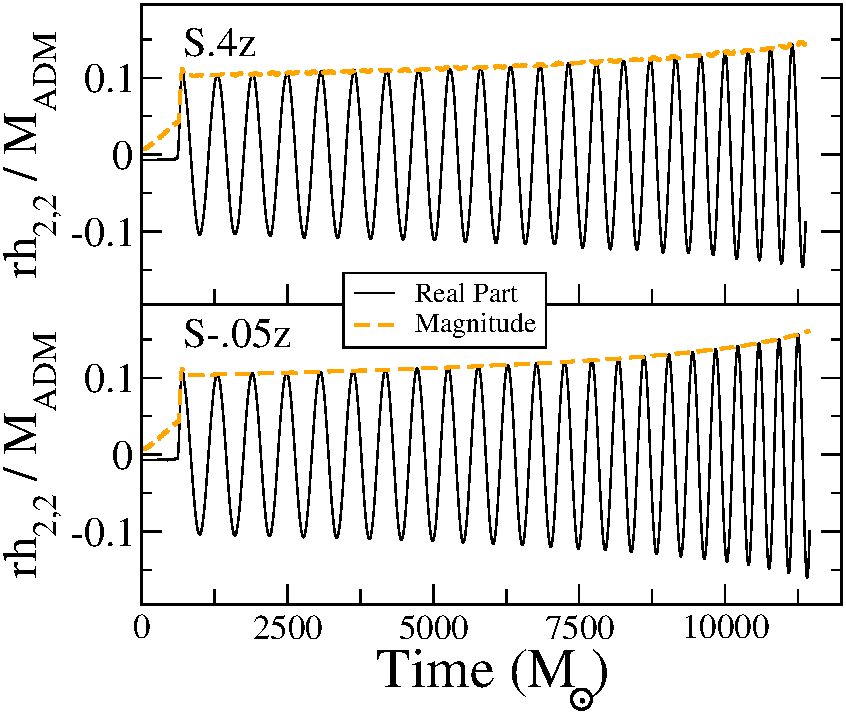
\includegraphics[width=0.95\columnwidth]{chap2/AlignedGW}
\caption[The gravitational waveforms for our anti-aligned and aligned runs.] { {\label{fig:AlignedGW}} The gravitational waveforms for our
  anti-aligned, {\tt S-.05z}, and aligned, {\tt S.4z} runs. The black curve
  represents the real part of the waveform, $\Re(h_{2,2})$ while the
  orange curve represents the magnitude of the waveform.}
\end{figure}
%%%%%%%%%%%%%%%%%%%%%%%%%%%%%%%%%%%%%%%%%%%%%%%%%%%%%%%%%%%%%%%%





%%%%%%%%%%%%%%%%%%%%%%%%%%%%%%%%%%%%%%%%%%%%%%%%%%%%%%%%%%%%%%%%
\begin{figure}
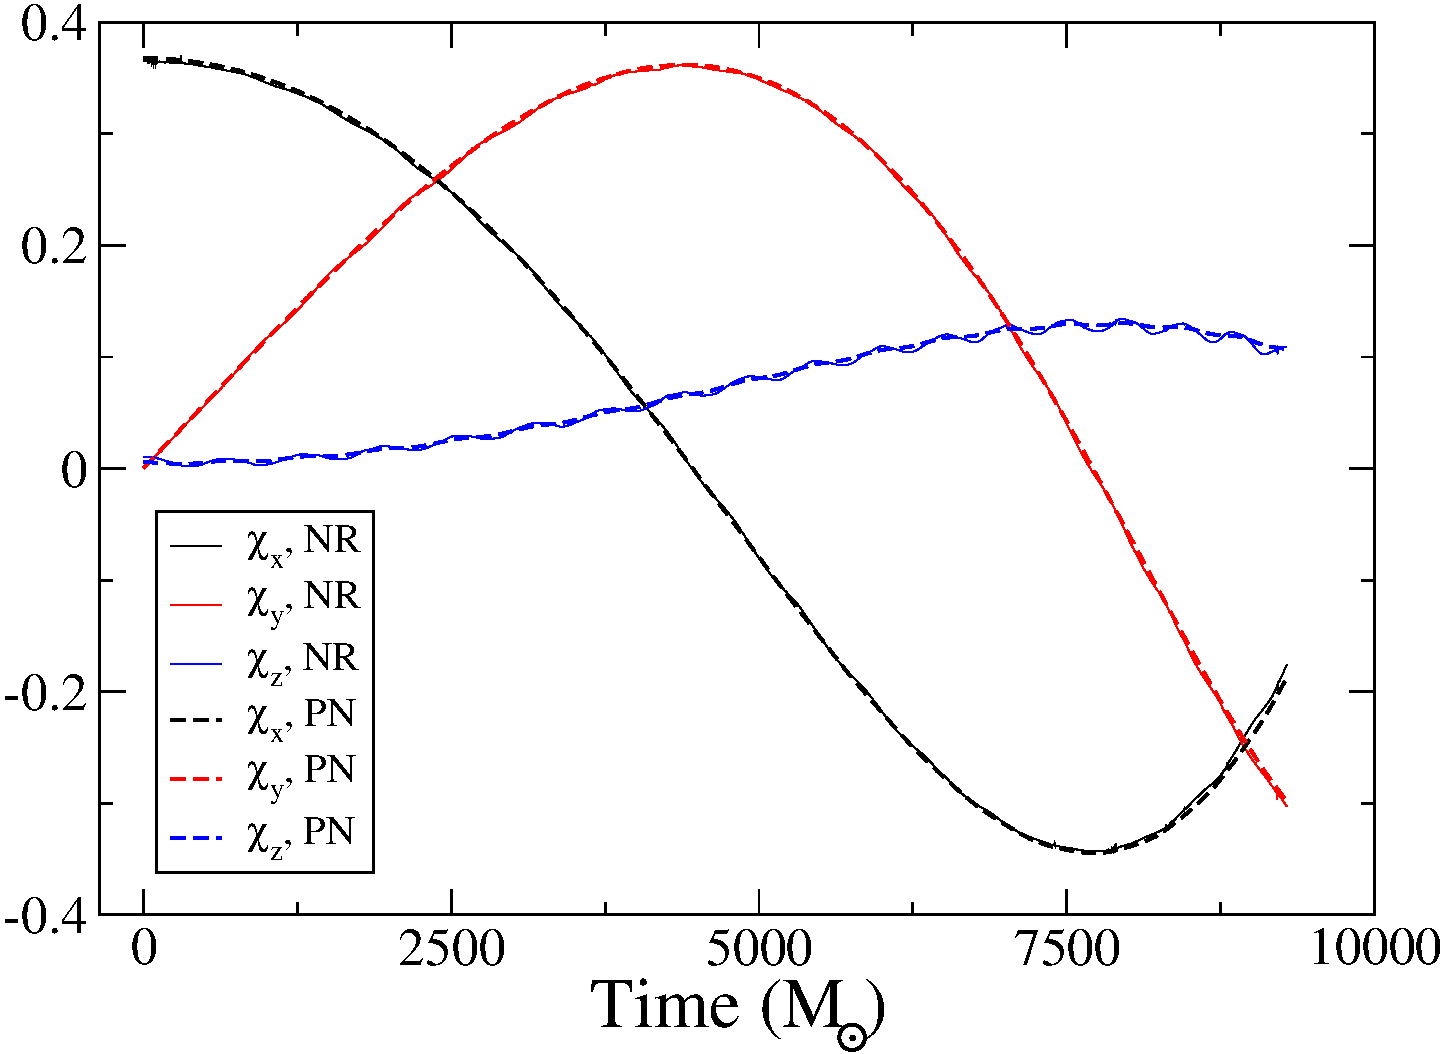
\includegraphics[width=0.95\columnwidth]{chap2/SpinMatchedUnmatched}
  \caption[Spin-components of one of the neutron stars during the precessing simulation.]{\label{fig:FullPrec} Spin-components of one of the neutron
    stars during the precessing simulation (thick, solid lines). The
    dotted and dashed lines represent the unmatched and matched PN
    results respectively. The agreement between PN and NR is good for
    both PN simulations. The orbital frequency was evolved using the
    Taylor T4 approximant. The matching was done in the interval
    [1892,4575].}
\end{figure}
%%%%%%%%%%%%%%%%%%%%%%%%%%%%%%%%%%%%%%%%%%%%%%%%%%%%%%%%%%%%%%%%

\subsection{Precession}


We now turn to the precessing simulation, {\tt S.4x}.
Figure~\ref{fig:FullPrec} shows the components of the spin-vector
$\vec\chi$ of one of the neutron stars, as a function of time. The
quasilocal spin diagnostic returns a spin with nearly constant
magnitude, varying only by $\pm 0.002$ around its average value
$0.370$. The spin components clearly precess, with the dominant
motion in the xy-plane (the initial orbital plane), with the
simulation completing about 2/3 of a precession cycle. A z-component
of the NS spin also appears, indicating precession of the neutron star
spin out of the initial orbital plane.

%%%%%%%%%%%%%%%%%%%%%%%%%%%%%%%%%%%%%%%%%%%%%%%%%%%%%%%%%%%%%%%%
\begin{figure}
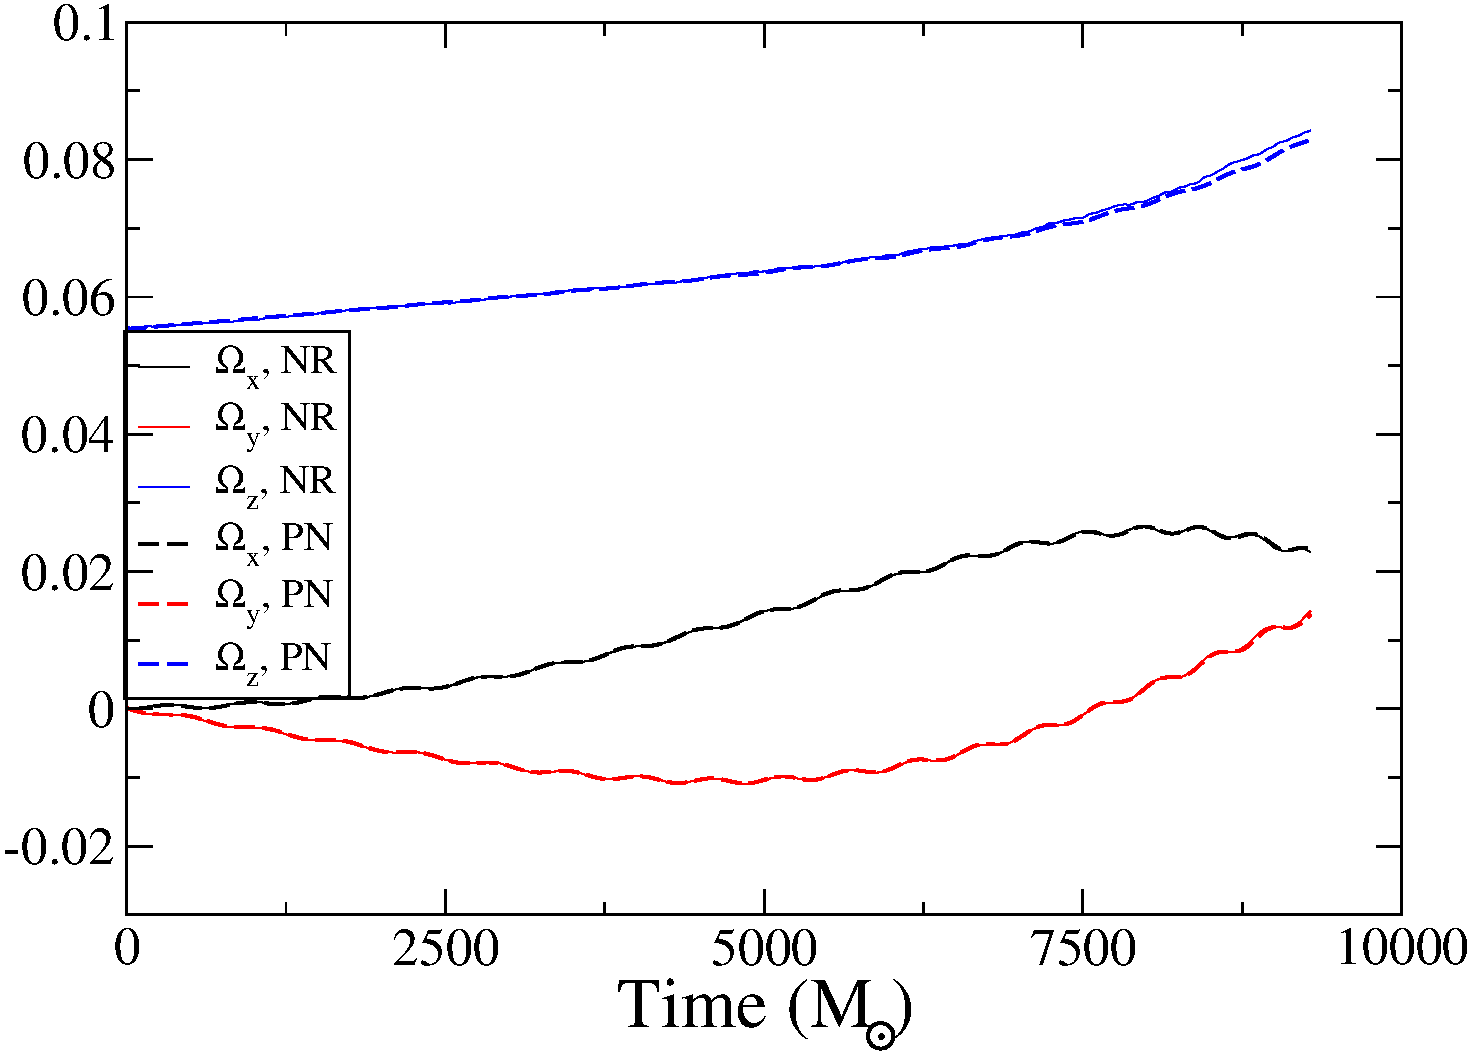
\includegraphics[width=0.95\columnwidth]{chap2/OmegaVectorMatchedUnmatched}
\caption[Components of the orbital frequency vectors during our evolutions.]{\label{fig:OmegaVectorComparison} Components of the orbital
  frequency vector $\vec\Omega$. Thick solid lines represent the
  precessing BNS simulation and thin
  dashed lines represent the matched  post-Newtonian simulations. The inclination reaches $\delta=0.34 {\rm rad}$ at $t=7600M_{\odot}$.}
\end{figure}
%%%%%%%%%%%%%%%%%%%%%%%%%%%%%%%%%%%%%%%%%%%%%%%%%%%%%%%%%%%%%%%%


Fig.~\ref{fig:FullPrec} shows a comparison of spin precession
  between numerical relativity and Post-Newtonain theory. We perform
  this comparison using
  the matching tecnhique in~\cite{OssokineEtAl:2014}. This gives very good agreement between PN
  (dotted) and NR (solid) as shown by Fig.~\ref{fig:FullPrec}. The NS spins indeed precess as expected,
  thus confirming both the quality of quasilocal spin measures, as
  well as the performance of the PN equations. Note that z-component of the spin in the NR data undergoes oscillations that are unmodelled by PN. These occur on a timescale of half the orbital timescale. Similar effects were found in~\cite{OssokineEtAl:2014}. The origin of these oscillations remains unclear.  The precession of the
  orbital angular frequency is shown in
  Fig.~\ref{fig:OmegaVectorComparison}. We find substantial
  precession away from the initial direction of the orbital frequency
  $\vec\Omega_0\propto \hat z$, with the angle $\delta$ between
  $\vec\Omega(t)$ and the z-axis reaching $20^\circ$. Once again,
  the PN equations reproduce the precession
  features successfully. 

\begin{figure}
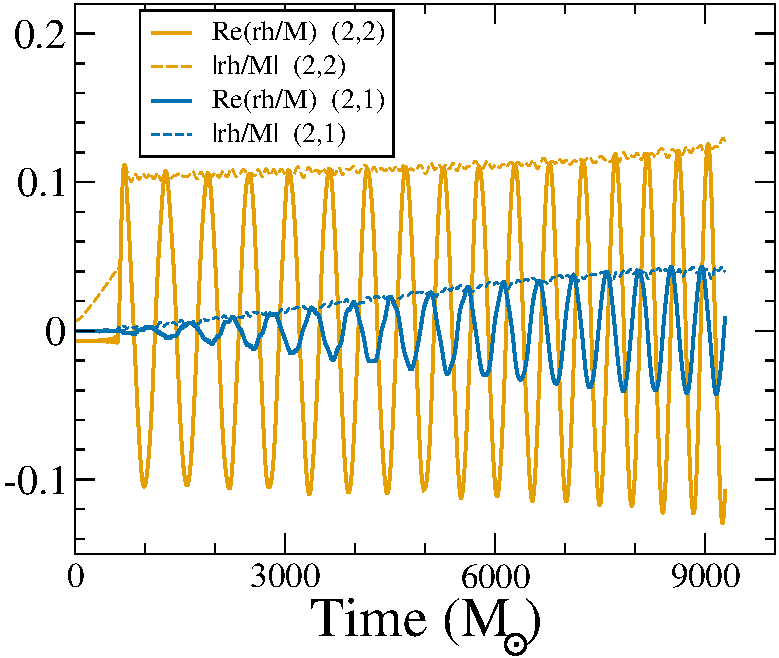
\includegraphics[width=0.9\columnwidth]{chap2/PrecGW}
\caption[Gravitational waveforms of our precessing run.]{\label{fig:PrecGW} Gravitational waveforms of our precessing
  run. Shown are the $(l,m)=(2,2)$ and $(2,1)$ modes, as extracted in
  a spherical harmonic decomposition aligned with the z-axis. The
  emergence of the (2,1) mode indicates precession of the orbital
  plane away from the xy-plane.}
\end{figure}


Finally, Fig.~\ref{fig:PrecGW} shows the (2,2) and the (2,1) spherical
harmonic modes of the gravitational wave-strain extracted at an
extraction surface of radius $R=647M_\odot$. The
(l,m)=(2,1) mode would be identically zero for an equal-mass aligned
spin binary with orbital frequency parallel to the z-axis, so the
emergence of this mode once again indicates precession in this binary.




%%%%%%%%%%%%%%%%%%%%%%%%%%%%%%%%%%%%%%%%%%%%%%%%%%%%%%%%%%%%%%%%
\subsection{Stellar Oscillations}
\label{sec:QNModes}
%%%%%%%%%%%%%%%%%%%%%%%%%%%%%%%%%%%%%%%%%%%%%%%%%%%%%%%%%%%%%%%%

\begin{figure}
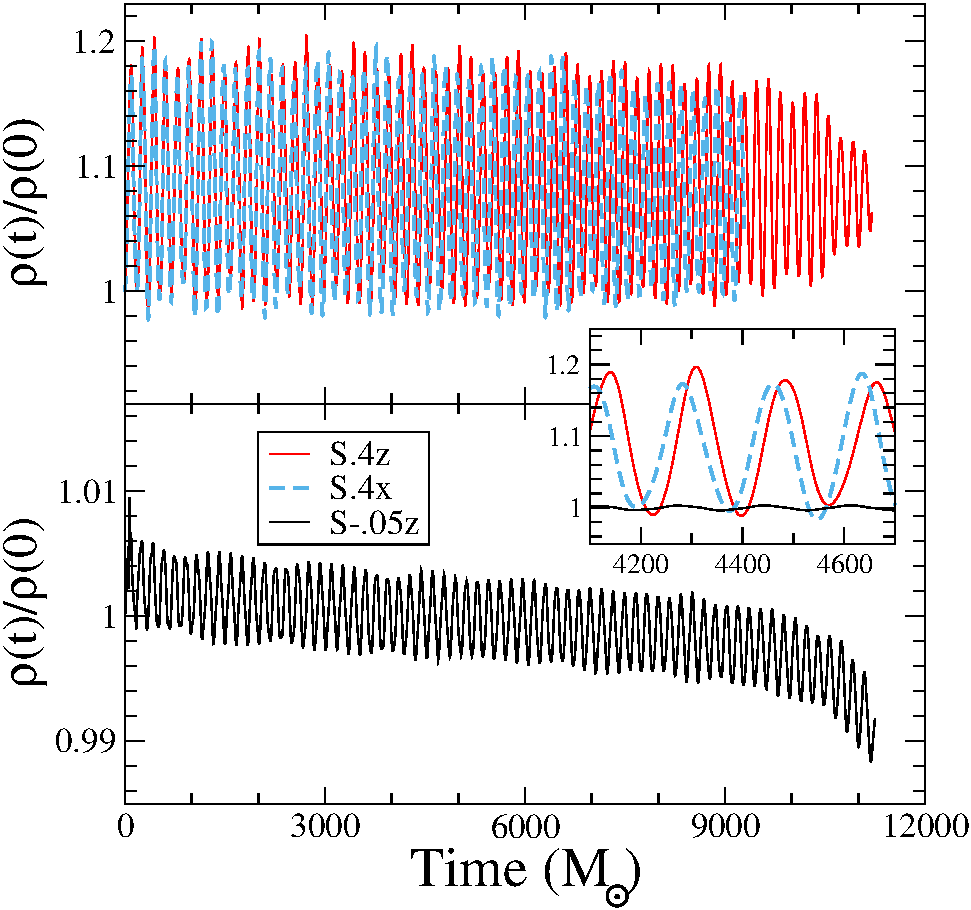
\includegraphics[width=0.95\columnwidth]{chap2/RhoMax}
\caption[The normalized maximum density in each of our runs.]{\label{fig:RhoMax} The maximum density $\rho(t)$ in each of
  our runs, normalized by the initial maximum density $\rho(0)$. The
  inset shows an enlargement of all three runs, illustrating that the
  oscillations are more pronounced in the high-spin simulations. }
\end{figure}

The rotating neutron stars constructed here show oscillations in the
central density, as plotted in Fig.~\ref{fig:RhoMax}. In the low spin
run, the density oscillations have a peak-to-peak amplitude of about
0.6\%, whereas in the high-spin runs ({\tt S.4z} and {\tt S.4x}), the density
oscillations reach a peak-to-peak amplitude of 20\%. The two
high-spin simulations show oscillations of nearly the same amplitude
and frequency, therefore oscillating nearly in phase throughout the
entire inspiral. The oscillation-period is about
$177 M_{\odot} \sim 0.87\rm{ms}$, i.e. giving a frequency of
$1.15{\rm kHz}$. It remains constant throughout the inspiral. The low-spin
run {\tt S-0.5z} exhibits a slightly smaller oscillation period of about
$P\approx 170M_{\odot}\approx 0.84\rm{ms}$, i.e. a frequency of
$\approx 1.19{\rm kHz}$. 


%%%%%%%%%%%%%%%%%%%%%%%%%%%%%%%%%%%%%%%%%%%%%%%%%%%%%%%%%%%%%%%%
\begin{figure}
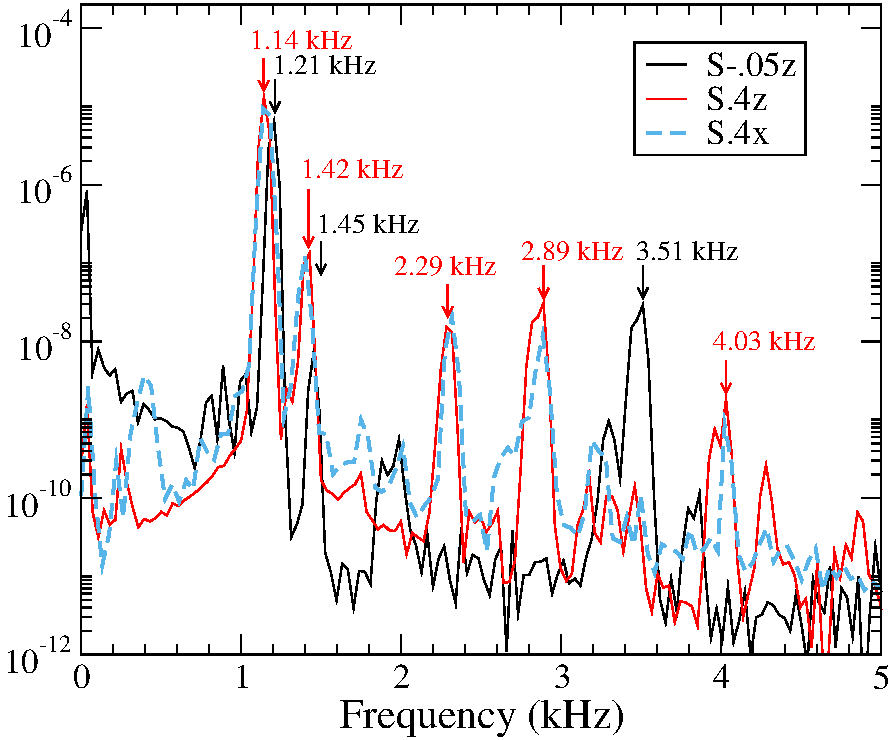
\includegraphics[width=0.95\columnwidth]{chap2/Density_FFT}
\caption[The Fourier transforms of the central density in all three of our runs.]{\label{fig:Density_FFT} The Fourier transforms of the central
  density in all three of our runs. Labelled are the peak frequencies
  for the quasi-radial F mode and the $l=2$, $^2f$ mode.}
\end{figure}
%%%%%%%%%%%%%%%%%%%%%%%%%%%%%%%%%%%%%%%%%%%%%%%%%%%%%%%%%%%%%%%%

To investigate the spectrum of the density oscillations, we perform a
Fourier-transform on $\rho(t)$. The result is shown in
Fig.~\ref{fig:Density_FFT}. The Fourier-transform confirms the
dominant frequencies just stated, and reveals several more frequency
components ranging up to 4kHz. The high spin evolutions {\tt S.4z} and
{\tt S.4x} exhibit identical freqencies for all five discernible peaks. In
contrast, the low-spin evolution {\tt S-.05z} shows different frequencies. 

We interpret these features as a collection of excited quasi-normal
modes in each neutron star. The modes are excited because the initial
data is not precisely in equilibrium. For the two high-spin cases the
neutron stars have similar spin, and therefore the same quasi-normal
modes, whereas in the low-spin model, the quasi-normal mode
frequencies differ due to the different magnitude of the spin.

To strengthen our interpretation, we consider the series of rotating,
relativistic, $\Gamma=2$ polytropes computed by~\cite{Dimmelmeier:2005zk}. 

~\cite{Dimmelmeier:2005zk}'s model ``AU3'' has a central density of
$1.074 \times 10^{-3} M_{\odot}^{-2}$ and its rotation is
quantified through the ratio of polar to equatorial radius,
$r_p/r_e = 0.780$.
Meanwhile, our high-spin runs have a central density of
$1.02 \times 10^{-3} M_{\odot}^{-2}$ (measured as time-average of the data shown in
Fig.~\ref{fig:RhoMax}) and from our initial data, we find
$r_p/r_e \sim 0.8$. Given the similarity in these
values, we expect~\cite{Dimmelmeier:2005zk}'s ``AU3'' to approximate our high-spin
stars {\tt S.4x}, {\tt S.4z}.
~\cite{Dimmelmeier:2005zk} reports a frequency of
$f_F=1.283\rm{kHz}$ for the spherically symmetric ($\ell=0$) F-mode,
and a frequency $f_{2f}=1.537\rm{kHz}$ for the axisymmetric $\ell=2$
mode $^2f$. These frequencies compare favorably with the two dominant
frequencies in Fig.~\ref{fig:Density_FFT}, $1.14\rm{kHz}$ and
$1.42\rm{kHz}$.

Presumably, the small differences in these frequencies can be
accounted for by the slight differences in stellar mass, radius, and
rotation. Moreover, tidal interactions and orbital motion could
factor in, as well. In our figure~\ref{fig:Density_FFT} we also see
several other peaks at higher frequencies, which are reminiscent of
the overtones and mode couplings in figure 10 of~\cite{Dimmelmeier:2005zk}. If we identify our peak at
  $f_{H1}=4.03\rm{kHz}$ with the $H_1$ mode, then (in analogy to
  ~\cite{Dimmelmeier:2005zk} Fig.~10), 
  $f_{H1}-f_{F}=(4.03-1.14)\rm{kHz}=2.89\rm{kHz}$, and
  $2f_{F}=2.28\rm{kHz}$, two frequencies that are indeed present in
  our simulations.
Although we find clear indications of axisymmetric $\ell=2$-modes,
we note that their power is smaller by two orders of magnitude,
compared to the spherically symmetric, dominant $F$ mode. 

Turning to the low-spin run {\tt S.05z}, we note that if, to first order,
these frequencies scale like $f\sim\sqrt{\rho}$ (on dimensional
grounds), then we expect to see $F=1.22\rm{kHz}$ and
$^2f=1.49\rm{kHz}$. This is very close to what is seen.


The density oscillations discussed in this section are reflected in
analogous oscillations in various other diagnostic quantities, for
instance, the orbital frequency, Fig.~\ref{fig:OmegaDotComparison} and
the quasilocal spin as shown in Fig.~\ref{fig:ChiVTDifferentRes2}.
The dominant frequencies $1.14\rm{kHz}$ and $1.42\rm{kHz}$ can be
robustly identified throughout our data analysis. In
figure~\ref{fig:ManyQuantities} we plot the Fourier transform of the
density, the $(2,0)$ and $(2,2)$ gravitational wave strains, the
orbital angular velocity time derivative $d\Omega/dt$ and the
measured spin $\chi$ for the {\tt S.4z} run. All show peaks in power at
these two frequencies, $F\sim1.14\rm{kHz}$ and $^2f\sim1.4\rm{kHz}$.
In simulations of eccentric, irrotational BNS systems,~\cite{Gold:2011df} find that the close encouters of the two stars excite f-modes in each star of frequency 1.586 kHz.

\begin{figure}
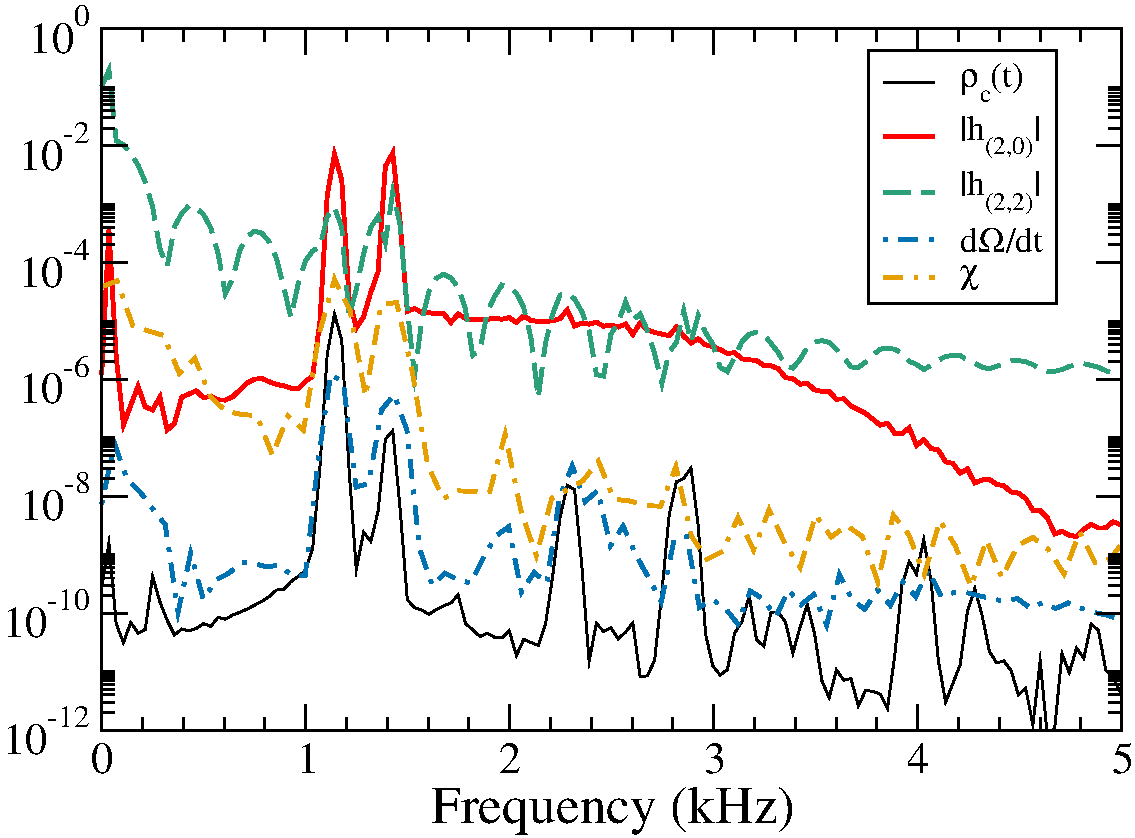
\includegraphics[width=0.95\columnwidth]{chap2/ManyQuantities}
\caption[Fourier transforms of several different quantities in the {\tt S.4z} run.]{\label{fig:ManyQuantities} Fourier transforms of the central
  density $\rho_c(t)$, two modes of the magnitude of gravitational wave strain
  $(|h_{2,2}|$ and $|h_{2,0}|$), $\dot{\Omega}$ and $\chi$ for the {\tt S.4z}
  run. All quantities show excess power at $1.14\rm{kHz}$ and
  $1.4\rm{kHz}$, corresponding to the frequencies of excited neutron
  star quasi-normal modes. 
}
\end{figure}



We believe  that the  stellar  modes are  excited because  the
  initial  data  are  not  in  perfect  equilibrium.  We  expect  the
  quasi-equilibrium  approximations   that  enter  the   initial  data
  formalism to become less valid  at higher spins, consistent with our
  observation that the high spin models exhibit stronger oscillations.
  This  interpretation is  strengthened by  additional simulations  of
  neutron stars at larger separation. Increasing   the  intial
  separation  by  a  factor  1.5,  while  keeping  the  same  rotation
  parameter  $\omega$  as  in  the  {\tt S.4z}-case,  we  find  quasi-normal
  oscillations   of  similar   amplitude  than   in  {\tt S.4z}.   If  the
  oscillations were  caused by  the neglect  of tidal  deformation, we
  would expect the amplitude to drop with the 3rd power of separation,
  inconsistent with our results. 


  Finally, we point out that the radial rotation profile,
  cf. Eq.~(\ref{eq:UniformRotation}) influences the amplitude of the
  induced quasi-normal oscillations. If the initial data is
  constructed with the rotation profile
  Eq.~(\ref{eq:ConformalUniformRotation}), instead of
  equation~\ref{eq:UniformRotation}, then the amplitude of the density oscillations for
  high spin doubles. This further supports our conjecture that the
  origin of this mode comes from non-equilibrium initial data.


\section{Conclusions}
\label{sec:Discussion}


In this chapter we implement Tichy's method~\citep{Tichy:2012rp} to
construct binary neutron star initial data with arbitrary rotation
rates. We demonstrate that our implementation is exponentially
convergent, as expected for the employed spectral methods.


We measure the spin of the resulting neutron stars using the
quasilocal angular momentum
formalism~\citep{BrownYork1993,Cook2007,Lovelace2008,OwenThesis}. The
resulting angular momentum is found to be nearly independent on the
precise choice of extraction sphere, cf. Fig.~\ref{fig:ChiVR}, and
provides a means to define the quasilocal angular momentum of each
neutron star to about 1\%, both in the initial data and during the
evolution, cf. Fig.~\ref{fig:ChiVTZoomed}. We are able to construct
binary neutron star initial data with dimensionless angular momentum
of each star as large as $\chi=S/M^2\sim 0.43$, both for the case of
aligned spins, and also for a precessing binary where the initial
neutron star spins are tangential to the initial orbital plane.

For irrotational BNS initial data sets, we find a quasilocal
  angular momentum of $\chi\sim 2\times 10^{-4}$,
  cf. Fig.~\ref{fig:ChiVOmega}. This spin is small enough that present
  waveform modeling studies for BNS
  (e.g.~\citep{Bernuzzi:2014owa,Baiotti2011,Baiotti:2010xh}) are not
  yet limited by residual spin.



When evolving the initial data sets, the dimensionless spin measured
in the initial data drops by about 0.004, and then remains constant
through the 10 inspiral orbits for which we evolved the neutron star
binaries. During these evolutions, we also demonstrated iterative
eccentricity removal: By analyzing the orbital frequency $\Omega(t)$
during the first few orbits, we can correct the initial data
parameters $\Omega_0$ and $\dot a_0$, and thus decrease the orbital
eccentricity from $e\approx 0.01$ to $e\lesssim 0.001$.



For the precessing simulation {\tt S.4x}, we find precession of the neutron
star spin directions. The numerically established precession of the
spin axes and of the orbital angular momentum agrees well with
post-Newtonian predictions.


The rotating neutron stars constructed here exhibit clear signals of
exciting quasi-normal modes. We are able to identify multiple modes
in the Fourier spectrum of the central density. The amplitude of the
excited quasi-normal modes increases steeply with rotation rate of the
neutron stars. For {\tt S-.05z} (spin magnitude $\chi=0.045$) the density
oscillations have peak-to-peak amplitude of 0.6\%, raising to 20\% for
the two runs with high spins ({\tt S.4x} and {\tt S.4z}).

{\it As discussed in the appendix below, the results presented in this chapter have since been updated due to the correction of a code error. Now, the density oscillations, for $\chi\sim 0.4$, have been decreased from $20\%$ to $0.5\%$, and the highest neutron star spin we can create has increased from $\chi\sim 0.43$ to $\chi\sim 0.65$. The full results are summarized below.}

%\section{Summary }
%
%\red{Write a summary.}

\begin{subappendices}
Chapter~\ref{chap:bns} presented a computational code for the
construction and evolution of binary neutron stars with arbitrary spin
vectors.
%
%\sout{In this erratum, we will revisit those results. Namely we have
%  found a computational error in the code that was used to generate
%  those results. We will begin by discussing what the error was and
%  what the general implications of that are. We will then revisit and
%  update the results of \cite{Tacik:2015tja} in lieu of this. Finally,
%  we will then discuss how the results of \cite{Tacik:2015tja} can be
%  pushed even further.}  
Following~\citep{Tichy:2012rp},
the 3-velocity of the neutron star fluid in an inspiraling binary is
written as the sum of an irrotational part and a rotational part,
\begin{equation}
U^i =
\frac{\Psi^{-4}\tilde{\gamma}^{ij}}{h\gamma_n}\left(\nabla_j\phi +
  W_j\right).
\end{equation}
Here $\Psi$ denotes the conformal factor, $\tilde{\gamma}_{ij}$ the
conformal spatial metric, $h$ the specific enthalpy, $\gamma_n$ the
Lorentz term $\gamma_n=\left(1-\gamma_{ij}U^iU^j\right)^{-1/2}$,
and $\phi$ the irrotational velocity potential. The vector $W_i$ represents a rotation
term designed to endow a uniform roation to the star,
\begin{equation}
\label{Eq:WVector}
W_i=\epsilon_{ijk}\omega^{j}r^k,
\end{equation}
where $\omega^j$ is the rotation vector chosen by hand, and $r^k$ is
the distance to the center of the star.
In this
construction, the solution of the Euler equation is
\begin{equation}
\label{Eq:EulerProper}
h=\sqrt{L^2-\left(\nabla_i\phi+W_i\right)\left(\nabla^i\phi+W^i\right)},
\end{equation}
where
\begin{equation}
L^2 = \frac{(x+y)+\sqrt{x^2+2xy}}{2\alpha^2},
\end{equation}
\begin{equation}
x=\left(\beta^i\nabla_i\phi+C\right)^2,
\end{equation}
and
\begin{equation}
\label{Eq:yProper}
y=2\alpha^2\left(\nabla_i\phi+W_i\right)W^i.
\end{equation}
Here $C$ denotes the Euler constant, $\alpha$ the lapse function and $\beta^i$ the shift-vector.

The code reported in Chapter~\ref{chap:bns} has a mistake in the
computation of $h$.  Instead of Eq.~\ref{Eq:EulerProper}, we computed
the following quantity.
\begin{equation}
h'=\sqrt{L^2-\left(\nabla_i\phi\right)\left(\nabla^i\phi\right)},
\end{equation}
and instead of Eq.~(\ref{Eq:yProper}), we computed
\begin{equation}
y'=\left(\nabla_i\phi+W_i\right)W^i.
\end{equation}

This error causes $h'$ to deviate from the correct $h$ by
\begin{align}
h'^2-h^2 =& 
\frac{\left(y'-y\right)}{2\alpha^2}+\frac{\sqrt{x^2+2xy'}-\sqrt{x^2+2xy}}{2\alpha^2} \nonumber \\
& +W_iW^i+2W^i\nabla_i\phi.
\end{align}
For non-rotating stars, $W^i=0$, the error dissapears: $h'\!=\!h$. 
In the limit of fast rotation, i.e. large $W$, we expect this difference
to be dominated by the terms quadratic in $W$,
\begin{equation}\label{eq:diff-h-high-W}
h'^2-h^2 \approx \frac{W^2}{2\alpha^2}.
\end{equation}
%The variable $\alpha\gtrsim 0.63$ in our data, so that $h'^2-h^2<0$.
%Therefore, in the rotating data-sets presented
%in~\cite{Tacik:2015tja}, the enthalpy was too low,
%The actual enthalpy $h$ of the constructed BNS was therefore smaller
%than the quantity $h'$ \nick{Can we re-word that?} implying a density
This implies the constructed BNS had an enthalpy
lower than the correct equilibrium configurations.  This picture is
consistent with Fig.~\ref{fig:RhoMax} (and
Fig.~\ref{fig:NewS4Density} below): for high NS spin, the central
density $\rho(t)$ immediately {\it increases} in an evolution, and
oscillates around values {\it larger} than the initial
density.

We now construct initial data with the same input parameters as for the case
{\tt S0.4z - Ecc3} in chap.~\ref{chap:bns}, and evolve it with the same
evolution code. For this evolution, we find:

\begin{enumerate}
\item Convergence of the Hamiltonian and Momentum constraints, and of the ADM energy and ADM angular momentum
  do not appreciably differ. Convergence of the neutron star spin is
  somewhat improved.

\item As noted in~\cite{0264-9381-11-2-015}, the absolute difference between the Komar mass $M_K$ and the
ADM energy $M_{\rm ADM}$ is an indicator of deviations from
equilibrium, as $M_K=M_{\rm ADM}$ for equilibrium systems in circular
orbits.
% At the highest resolution, this difference is
%$2.6\times10^{-3}$ for the incorrect initial data, and
%$2.1\times10^{-4}$ for the corrected initial data.
The difference between  the Komar mass $M_K$ and ADM energy $E_{\rm
  ADM}$ is reduced by an order of magnitude, from $|M'_K-M'_{\rm
  ADM}|=2.6\times10^{-3}$ to $|M_K-M_{\rm ADM}|=2.1\times10^{-4}$.
This supports the
idea that the neutron stars themselves are closer to being in
equilibrium.

\item Evolution of the corrected initial data yields substantially
  smaller density oscillations. Figure~\ref{fig:NewS4Density} shows the
density oscillations for the evolution reported in chap.~\ref{chap:bns}
and for the evolution of the corrected initial data.  Peak-to-peak
density oscillations are reduced from $\sim 20\%$ to about $0.5\%$.
Density oscillations of $\sim 0.5\%$ also occur in our simulations of
non-spinning binary neutron stars.
The frequency of density-oscillation is
unchanged, consistent with our interpretation that it represents a
quasi-normal mode. We note that the phase of oscillation has changed
by approximately half of a period.

\begin{figure}
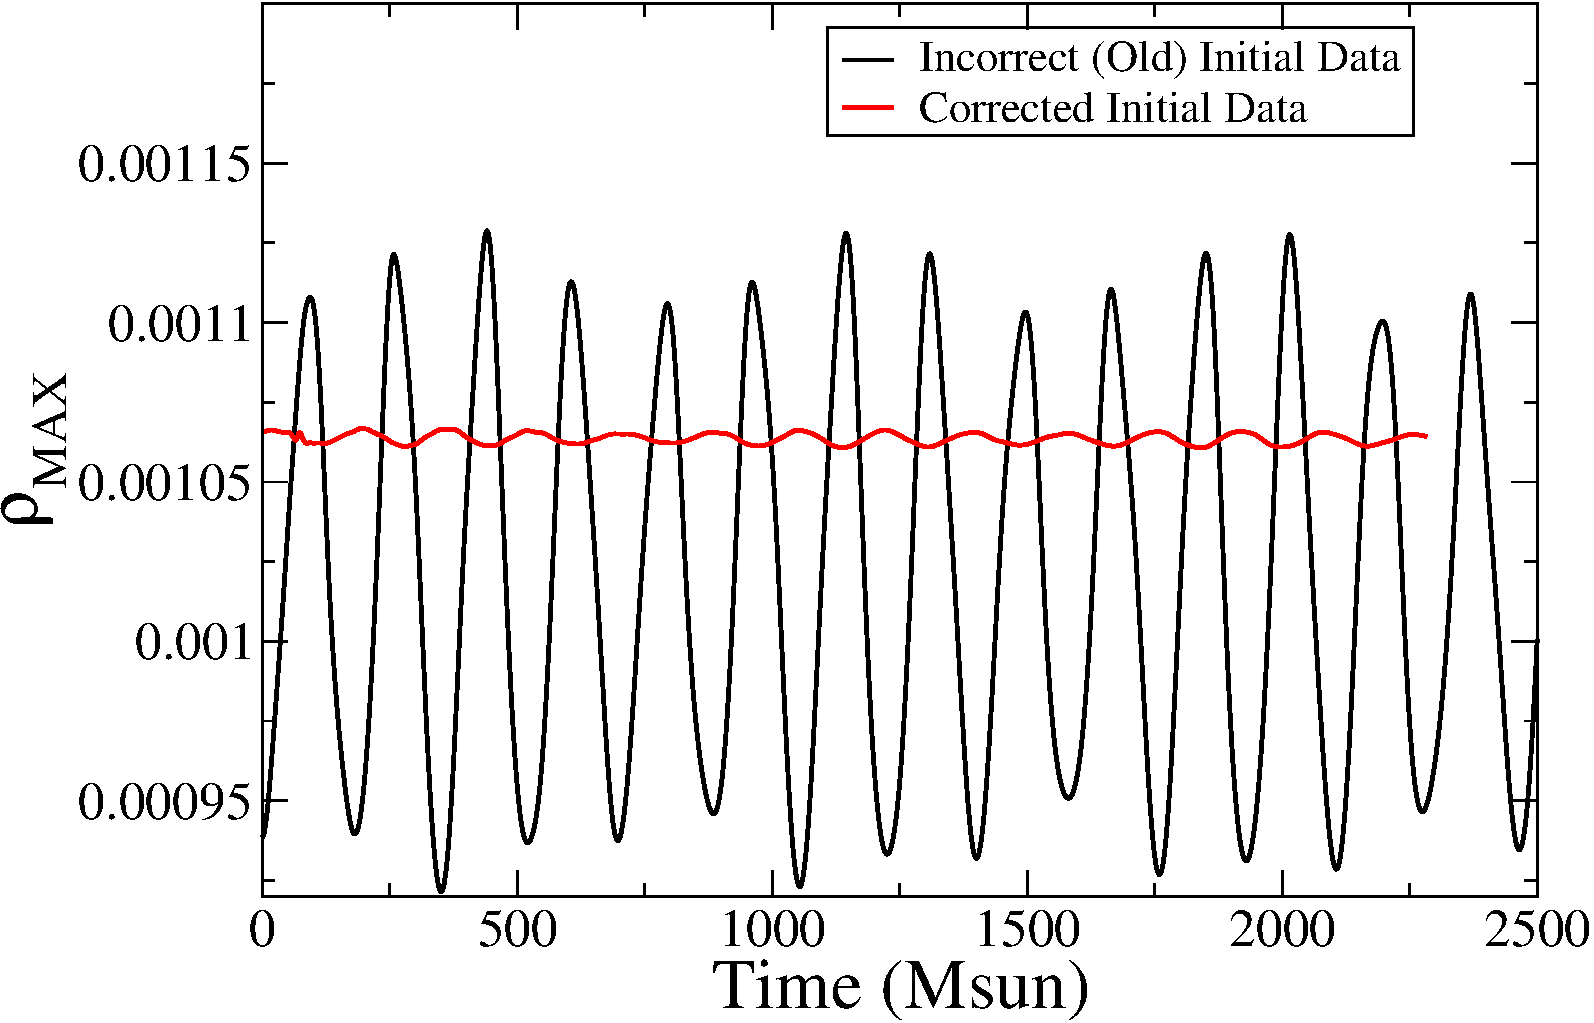
\includegraphics[width=0.95\columnwidth]{chap2/NewS4Density}
\caption[Density oscillations with corrected initial data.]{\label{fig:NewS4Density}Density oscillations for
  the {\tt S0.4z} run from chap.~\ref{chap:bns} and a new evolution of
  the corrected initial data.
}
\end{figure}

\item 
The orbital frequency $\Omega(t)$ has significantly
  smaller oscillations at periods $\approx 200M_{\odot}$.
Figure~\ref{fig:NewDOmegaVT} compares $\dot{\Omega}(t)$ between evolutions of the old (erroneous) and
new (corrected) initial data.  High-frequency oscillations are strongly suppressed with the
corrected initial data, allowing a clearer view of the lower-frequency
sinusoidal features which are due to the overall trajectory of the
binary. 


\begin{figure}
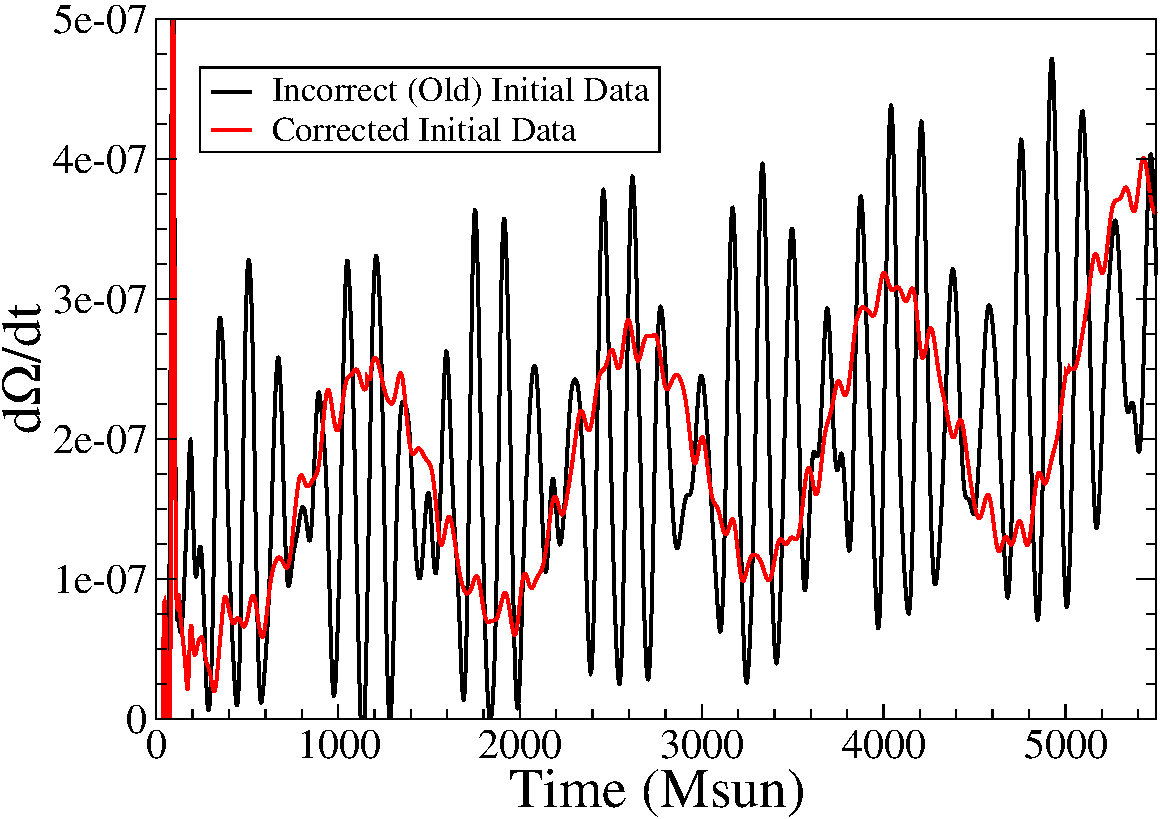
\includegraphics[width=0.95\columnwidth]{chap2/NewDOmegaVT}
\caption[Derivative of orbital angular frequency with corrected initial data.]{\label{fig:NewDOmegaVT} Derivative of the orbital angular
  frequency from the S0.4z run from chap.~\ref{chap:bns} and from a
  new run with the same parameters.}
\end{figure}

\item The corrected code yields higher central density and therefore more
compact stars (at same mass).  At the same rotational frequency
parameter $\omega$ (as defined in Eq.~\ref{Eq:WVector}) we therefore expect the corrected code to yield
stars with smaller angular momentum.  This is indeed the case as is
shown in Fig.~\ref{fig:NewS4Spin}. The subsequent evolution of the
spin magnitude is comparable for both incorrect and corrected initial
data (cf. inset of Fig.~\ref{fig:NewS4Spin}) although the oscillations present in the data are reduced. 

\begin{figure}
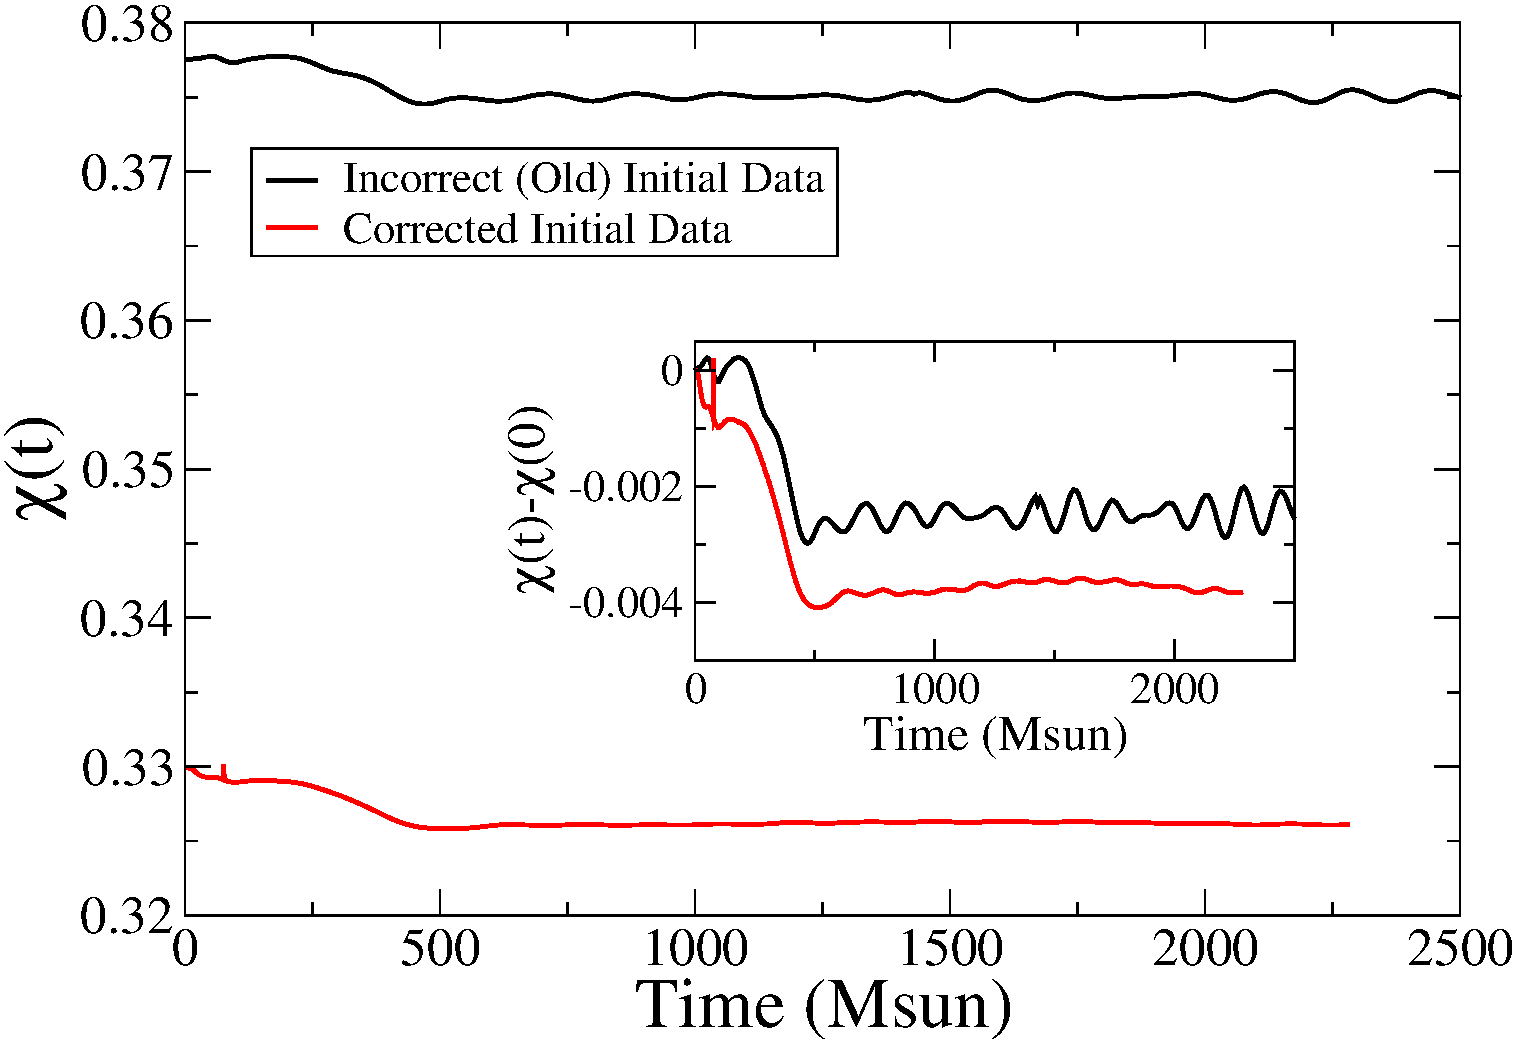
\includegraphics[width=0.95\columnwidth]{chap2/NewS4Spin}
\caption[Dimensionless spin during the evolution of corrected initial data.]{\label{fig:NewS4Spin} Dimensionless spin,
  $\chi=J/M_{\rm ADM}^2$, measured during the
  evolution of the S0.4z-Ecc3 run, computed from old and corrected initial data.
  The inset subtracts the value of the spin at $t=0$ from both curves.
}
\end{figure}
\end{enumerate}

We also find that the corrected code is capable of
  solving initial data sets for higher values of the NS rotation
  parameter $\omega$.  Figure~\ref{fig:NewS4Spin} already showed that
at the same rotation parameter $\omega$, the corrected code yields
smaller spin. Computing a sequence of initial data sets at different
$\omega$, we obtain Figure~\ref{fig:NewChiVOmega}.
For small $\omega$, the $\chi(\omega)$ relation is unchangeindicating that the low-spin evolution reported in~\cite{Tacik:2015tja} is probably only mildly affected.  For large $\omega$,
 the initial data solver can create ID at spins up to
$\chi\sim 0.63$, a factor $\sim 1.4$ larger than the erroneous code. This is, in fact, greater than the break-up spin of $\chi=0.57$
found for $\Gamma=2$ polytropes found in~\cite{Ansorg:2003br}.

%%%%%%%%%%%%%%%%%%%%%%%%%%%%%%%%%%%%%%%%%%%%%%%%%%%%%%%%%%%%%%%%
\begin{figure}
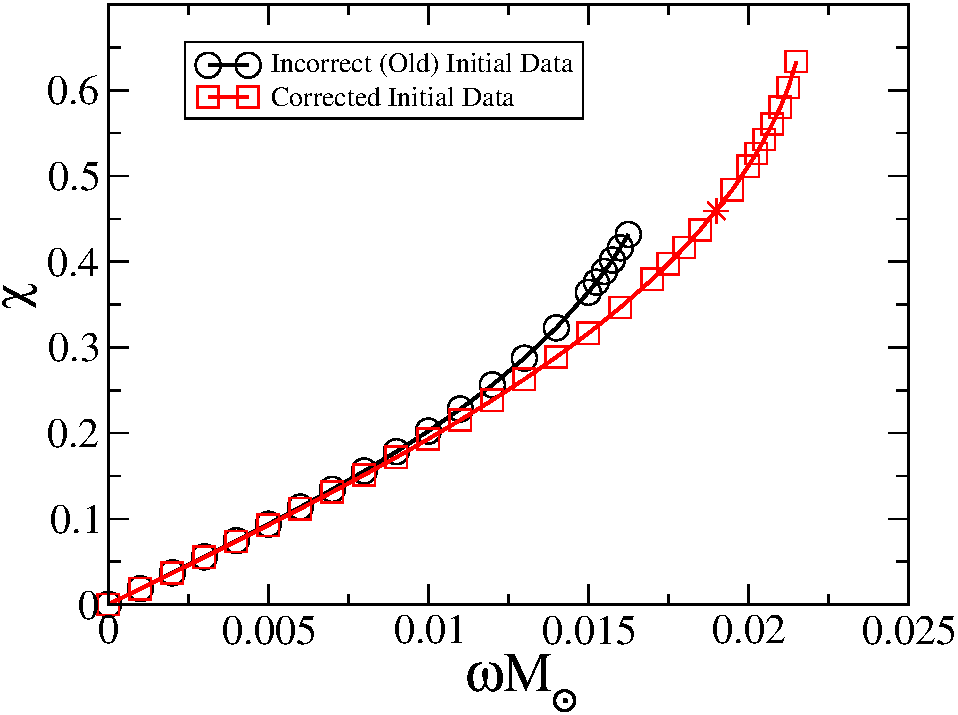
\includegraphics[width=0.95\columnwidth]{chap2/NewChiVOmega}
\caption[$\chi$ vs. $\omega$ relation with corrected initial data.]{\label{fig:NewChiVOmega} $\chi$ as a function of $\omega$ in
  the initial data. The black curve is from Fig. 8 of
  \cite{Tacik:2015tja}, while the red curve is generated with the
  corrected initial data. The astericks indicates the configuration we
evolve in Fig.~\ref{fig:Ev1Snapshot}.}
\end{figure}
%%%%%%%%%%%%%%%%%%%%%%%%%%%%%%%%%%%%%%%%%%%%%%%%%%%%%%%%%%%%%%%%

Being now able to construct ID at larger NS spins, we evolve 
an equal-mass, equal-spin ID
set with $\omega=0.019M_{\odot}^{-1}$, $\chi=0.46$. In
figure~\ref{fig:Ev1Snapshot} we present a snapshot of the run,
plotting the normalized density oscillations, spin, and the
trajectories of the stars. The peak-to-peak density oscillations are now about
$2\%$, higher than in the $\chi\sim0.33$ evolution, but still much
smaller than for the erroneuous initial data despite the larger NS spin.
\begin{figure}
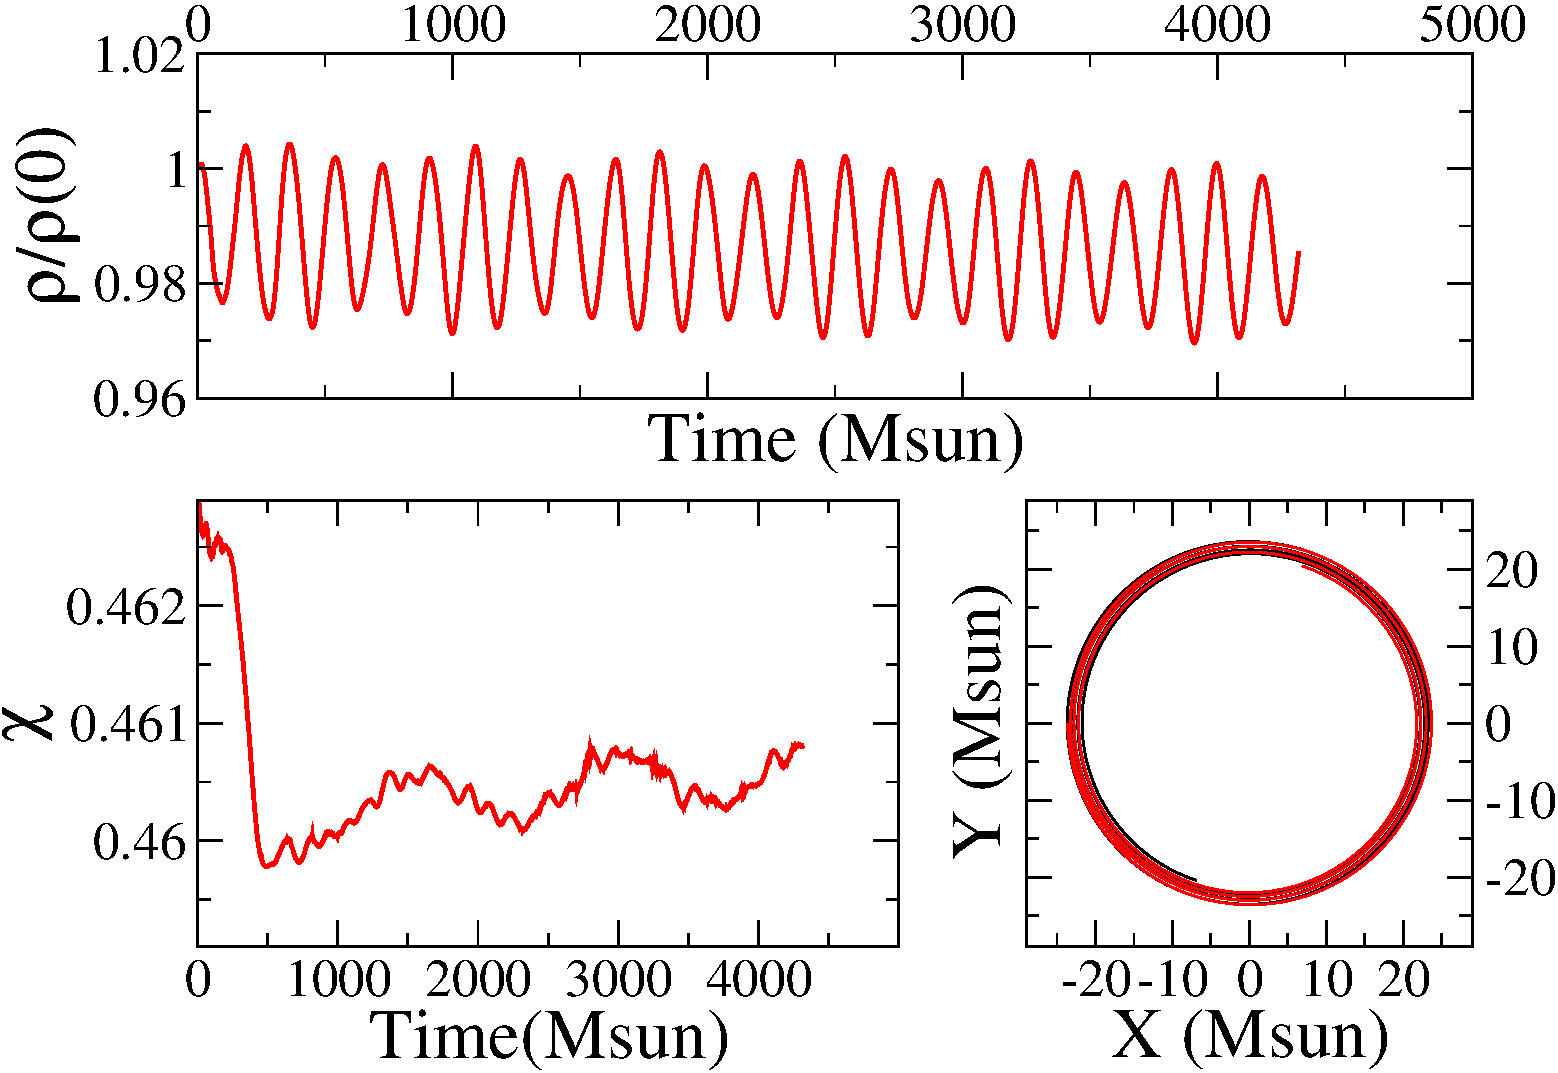
\includegraphics[width=0.95\columnwidth]{chap2/Ev1Snapshot}
\caption[Snapshot of a high-spin evolution using corrected initial data.]{\label{fig:Ev1Snapshot} A snapshot of an evolution with
  $\omega=0.019$. The top panel shows the normalized density
  oscillations. The bottom-left panel shows the measured spin of a
  star. The bottom-right panel shows the orbtis of the stars as they
  inspiral.}
\end{figure}
\end{subappendices}

%\chapter{Gravitational and Electromagnetic Radiation from Spinning Magnetized Binary Neutron Stars}

\section{Chapter Overview}

{\bf Below is a bullet list of things to include in this chapter.}
\begin{itemize}
\item Motivations - what are the luminosities we expect. Pulsar, single magnetized star, double magnetized stars.
\item Initial data we constructed. What parameters and why. Convergence thereof.
\item Results?
\end{itemize}

\section{Introduction}

My Introduction

\section{Initial Data}



\section{Summary }

My Summary.

\chapter[Initial Data for BH-NS Binaries, with Rotating Stars]{Initial Data for Black Hole--Neutron Star Binaries, with Rotating Stars}
\label{chap:bhns}

{\it The material in this chapter is based on "Initial data for black hole--neutron star binaries, with rotating stars" by Nick Tacik et al. Submitted to Classical and Quantum Gravity. arXiv:1607.07962}

\section{Chapter Summary}
  The coalescence of a neutron star with a black hole is a primary
  science target of ground-based gravitational wave detectors.
  Constraining or measuring the neutron star spin directly from
  gravitational wave observations requires knowledge of the dependence of
  the emission properties of these systems on the neutron star spin.
  This chapter lays foundations for this task, by developing a numerical
  method to construct initial data for black hole--neutron star
  binaries with arbitrary spin on the neutron star. We demonstrate
  the robustness of the code by constructing initial-data sets in
  large regions of the parameter space. In addition to varying the
  neutron star spin-magnitude and spin-direction, we also explore
  neutron star compactness, mass-ratio, black hole spin, and black
  hole spin-direction. Specifically, we are able to construct initial
  data sets with neutron stars spinning near centrifugal break-up, and
  with black hole spins as large as $S_{\rm BH}/M_{\rm BH}^2=0.99$.



%\submitto{\CQG}


%%%%%%%%%%%%%%%%%%%%%%%%%%%%%%%%%%%%%%%%%%%%%%%%%%%%%%%%%%%%%%%%
\section{Introduction}
\label{sec:Introduction}
%%%%%%%%%%%%%%%%%%%%%%%%%%%%%%%%%%%%%%%%%%%%%%%%%%%%%%%%%%%%%%%%


The spectacular detection of merging binary black holes by Advanced
LIGO~\citep{Abbott:2016nmj,LIGOVirgo2016a} marks the beginning of the
era of gravitational wave astronomy. With binary black holes detected
through gravitational waves, and binary neutron stars known from radio
observations~\citep{Hulse:1975uf}, mixed black-hole - neutron star
(BH-NS) binaries are now the only compact object binary whose
existence has not yet been directly observed.

BH-NS systems are an important potential source of gravitational waves
for advanced ground-based detectors, with an expected event rate of
approximately ten per year~\citep{AbadieLSC:2010}, albeit with a large
uncertainity. In addition to gravitational waves, BH-NS mergers can
be an important source of electromagnetic radiation~\citep{Li:1998bw,Roberts2011,metzger:11,2013MNRAS.430.2121P,2013MNRAS.430.2585R,2014ApJ...780...31T}
 and give further clues to
the violent processes that occur during the merger. If a massive disk
is left from the merger, for instance, it could lead to a
short-duration gamma ray burst (SGRB) and material ejected during the
merger could radiate a signal such as a "kilonova"~\citep{metzger:11}.

Direct numerical solutions are one of the primary means to explore
coalescing compact object binaries
(e.g.~\cite{baumgarteShapiroBook,2014ARA&A..52..661L,Pfeiffer:2012pc}).
Such simulations are important to accurately study both the
gravitational waves and electromagnetic emission produced by compact
object mergers. Fully general relativistic simulations of mixed BH-NS
binaries have been performed for about 10
years~\citep{Shibata:2006bs,Faber2005} investigating the importance of
mass-ratio~\citep{Foucart:2014nda,Foucart:2013psa,FoucartEtAl:2011},
black hole
spin~\citep{East:2011xa,Shibata:2006ks,Foucart:2013a,Foucart:2010eq,Kawaguchi:2015,Etienne:2008re},
eccentricity~\citep{East:2015yea,2012PhRvD..85l4009E,Stephens:2011as}, equations of state~\citep{Duez:2009yy,Kyutoku:2010zd,Kawaguchi:2015,Foucart:2013a},
magnetic
fields~\citep{Chawla:2010sw,Paschalidis2014,Kiuchi:2015qua,2012PhRvD..85f4029E,Etienne:2012te},
neutrino physics~\citep{Foucart:2015a}, disk
formation~\citep{Lovelace:2013vma,Shibata:2007zm,Pannarale:2015jia},
outflows~\citep{Deaton2013,Kyutoku:2013wxa} and electromagnetic
emission signatures~\citep{PaschalidisEtAl:2013,Kawaguchi:2016}.

The parameter space for BH-NS binary simulations is relatively
large. The mass ratio, $q$, NS compactness, $C$, and black hole spin, $\vec{\chi}$, have
been of particular interest in numerical simulations, because they
have the most profound impact of the evolution of the binary, and are the primary 
variables to control whether the neutron star tidally disrupts~\citep{Foucart2012}.
One aspect that has not been studied, however, is the effect of
neutron star spin. With the exceptions of~\cite{Shibata:2006bs,East:2015yea}, all
simulations to date use irrotational neutron stars in their BH-NS
binaries. For NS-NS binaries, in constrast, a significant number of
studies investigate spinning neutron
stars~\citep{Baumgarte:2009fw,Tichy:2011gw,East:2012zn,Tichy:2012rp,Bernuzzi:2013rza,Kastaun:2013mv,Tsatsin:2013jca,Dietrich:2015pxa,East:2015yea,Tsokaros:2015fea,Tacik:2015tja}. Since
no BH-NS binaries have been directly observed, the NS spins are, at
least observationally, unconstrained. A spinning neutron star will
affect the gravitational waveforms and cause the inspiral to proceed
more slowly (for spin-aligned NS). The spin can be important for
gravitational wave detection and can cause appreciable mismatch with
non-spinning templates, especially at lower BH-NS mass ratios~\citep{Ajith:2011ec}. We also expect the spin to also affect the time of
NS disruption, as the stellar material will be less tightly bound to
the stellar surface.


Any evolution must start with initial data, and so in this chapter, we
consider the construction of fully general-relativistic initial data
sets for BH-NS binaries with generic spin on the neutron star. We
combine the techniques of constructing BH-NS initial data without
NS-spin~\citep{FoucartEtAl:2008,Henriksson:2014tba} with the
rotating-NS formalism developed by ~\cite{Tichy:2012rp} as
implemented in ~\cite{Tacik:2015tja} (cf. chap.~\ref{chap:bns}). We show that this
approach, implemented in the Spectral Einstein Code {\tt
  SpEC}\footnote{http://www.black-holes.org/SpEC.html}, is robust and can construct BH-NS binaries
with NS spin magnitudes up to nearly rotational break-up
(dimensionless spin $\chi_{\rm NS}\sim 0.7$) and arbitrary rotation axis.
The code also successfully constructs binaries with mass-ratios
from 2 to 10, and with black hole spins $0\le \chi_{\rm BH}\le 0.99$.

The structure of this article is as follows: In
section~\ref{sec:BH-NSIDF}, we review the standard numerical
relativity initial data formalism, as well as the formalism developed
in~\cite{Tichy:2011gw} to create binaries with spinning NS, and
discuss how this is extended to BH-NS systems. In
section~\ref{sec:BHNSNumMethods} we discuss the numerical methods used
by our initial data solver. In section~\ref{sec:BHNSResults}, we
create a number of initial data sets to demonstrate the robustness of
our solver by constructing BH-NS initial data sets with various values
of neutron star spin, black hole spin, and mass ratio. We conclude
with a discussion in section~\ref{sec:Conc}. Throughout this article
we use units where $G=c=M_{\odot}=1$.

%%%%%%%%%%%%%%%%%%%%%%%%%%%%%%%%%%%%%%%%%%%%%%%%%%%%%%%%%%%%%%%%
\section{Initial Data Formalism}
\label{sec:BH-NSIDF}
%%%%%%%%%%%%%%%%%%%%%%%%%%%%%%%%%%%%%%%%%%%%%%%%%%%%%%%%%%%%%%%%



In this section we will discuss the formalism used to solve the
Einstein field equations and create quasi-equilibrium initial data for
BH-NS binaries with spinning neutron stars. We employ the
extended-conformal thin-sandwich
formalism~\citep{Pfeiffer2003b,York1999} to cast the Einstein
constraint equations as a set of elliptic equations. Neutron star
spin is incorporated with the approach developed
in~\cite{Tichy:2011gw}, and the equations are solved by a
generalization of the initial data solver developed
in~\cite{FoucartEtAl:2008}.


We begin with the $3+1$ decomposition of the space-time metric
tensor,
\begin{equation}
g_{\mu\nu}dx^{\mu}dx^{\nu} = -\alpha^2dt^2 + \gamma_{ij}\left(dx^i +
  \beta^idt\right)\left(dx^j+\beta^jdt\right),
\end{equation}
where $\alpha$ is the lapse function, $\beta^i$ is the shift vector,
and $\gamma_{ij}$ is the induced metric on a spatial hypersurface
$\Sigma(t)$. The normal vector $n^{\mu}$ to $\Sigma(t)$ is related to
the coordinate time $t$ by $ t^{\mu} = \alpha n^{\mu} + \beta^{\mu}$.
The extrinsic curvature of $\Sigma(t)$ is given by
$ K_{\mu\nu} = -\frac{1}{2}\mathcal{L}_n\gamma_{\mu\nu}$, where
$\gamma_{\mu\nu}=g_{\mu\nu}+figuren_{\mu}n_{\nu}$ and $\mathcal{L}_n$ is the
Lie derivative in the direction of $n^{\mu}$. By construction
$K_{\mu\nu} $ is a purely spatial tensor by construction,
i.e. $K_{\mu\nu}n^\mu=0=K_{\nu\mu}n^\mu$, and so we restrict our
attention to the spatial part of the extrinsic curvature, $K^{ij}$. It
is convenient to decompose it into its trace and trace-free parts,
\begin{equation}
K^{ij} = A^{ij}+\frac{1}{3}K\gamma_{ij}.
\end{equation}
The matter in the system is modelled with the stress-energy tensor of
a perfect fluid 
\begin{equation}
T_{\mu\nu}=\left(\rho+P\right)u_{\mu}u_{\nu}+Pg_{\mu\nu},
\end{equation}
where $\rho$ is the fluid's energy density, $P$ is its pressure, and
$u^{\mu}$ is its four-velocity. It is further useful to define the
projections of the matter quantities,
\begin{eqnarray}
E &=& T^{\mu\nu}n_{\mu}n_{\nu},\\
S &=& \gamma^{ij}\gamma_{i\mu}\gamma_{j\nu}T^{\mu\nu}, \\
J^i &=& -\gamma^{i}_{\mu}T^{\mu\nu}n_{\nu}.
\end{eqnarray}
The spatial metric is conformally scaled,
\begin{equation}
\gamma_{ij}=\Psi^4\tilde{\gamma}_{ij},
\end{equation}
where $\Psi$ denotes the conformal factor and $\tilde{\gamma}_{ij}$
the conformal metric. Other quantities are conformally scaled as follows:
\begin{eqnarray}
E &=& \Psi^{-6}\tilde{E}, \\
S &=& \Psi^{-6}\tilde{S}, \\
J^i &=& \Psi^{-6}\tilde{J}^i, \\
A^{ij} &=& \Psi^{-10}\tilde{A}^{ij}, \\
\alpha &=& \Psi^{6}\tilde{\alpha}. 
\end{eqnarray}
$\tilde{A}^{ij}$ is related to the shift and to the time derivative of
the conformal metric, $\tilde{u}_{ij}=\partial_t\tilde{\gamma}_{ij}$,
by
\begin{equation}
\tilde{A}^{ij} =
\frac{1}{2\tilde{\alpha}}\left[\left(\tilde{\mathrm{L}}\beta\right)^{ij}-\tilde{u}^{ij}\right],
\end{equation}
where $\tilde{\mathrm{L}}$ is the conformal longitudinal operator,
\begin{equation}
\left(\tilde{\mathrm{L}}V\right)^{ij}=\tilde{\nabla}^iV^j + \tilde{\nabla}^jV^i
- \frac{2}{3}\tilde{\gamma}^{ij}\tilde{\nabla}_kV^k.
\end{equation}
With these definitions and conformal rescalings, the Einstein
constraint equations, and the Einstein evolution equation for the
trace of the extrinsic curvature yield a set of five coupled elliptic
equations, called the extended conformal thin sandwich (XCTS)
equations~\citep{Pfeiffer2003b}. They are written in the form


\begin{eqnarray}
\label{eq:XCTS-ConformalFactor}
%\fl
\tilde{\nabla}^2\Psi - \frac{1}{8}\Psi\tilde{R} -
\frac{1}{12}\Psi^5K^2 
+\frac{1}{8}\Psi^{-7}\tilde{A}_{ij}\tilde{A}^{ij} &=-2\pi\Psi^{-1}\tilde{E},\\
\label{eq:XCTS-Shift}
%\fl
2\tilde{\alpha}\bigg[\tilde{\nabla}_j\left(\frac{1}{2\tilde{\alpha}}\big(\tilde{L}\beta\big)^{ij}\right)-\tilde{\nabla}_j\left(\frac{1}{2\tilde{\alpha}}\tilde{u}^{ij}\right)
-\frac{2}{3}\Psi^6\tilde{\nabla}^iK\bigg] &=16\pi\tilde\alpha\Psi^4\tilde{J}^i,\\
%\fl 
\tilde{\nabla}^2\left(\tilde{\alpha}\Psi^7\right) -
\left(\tilde{\alpha}\Psi^7\right)\bigg[\frac{1}{8}\tilde{R}+\frac{5}{12}\Psi^4K^2+\frac{7}{8}\Psi^{-8}\tilde{A}_{ij}\tilde{A}^{ij} 
\bigg] \nonumber \\
\qquad\qquad\qquad\qquad+\Psi^5\left(\partial_{t}K- \beta^{k}\partial_kK\right)&=-2\pi\tilde\alpha\Psi^{5}\big(\tilde{E}+2\tilde{S}\big).
\label{eq:XCTS-Lapse}
\end{eqnarray}
These equations are solved for the conformal factor, $\Psi$, the
shift, $\beta^i$, and the densitized lapse, $\tilde\alpha\Psi^7$.
Equations~(\ref{eq:XCTS-ConformalFactor})--(\ref{eq:XCTS-Lapse})
constitute the gravitational sector of the initial data construction.
The free data are $\tilde{\gamma}_{ij}$, $\tilde{u}_{ij}$, $K$ and
$\partial_t K$. Since we will be constructing initial data in a
corotating coordinate system, the free data corresponding to
time-derivatives can be naturally set to zero:
$\tilde{u}_{ij}=\partial_t K=0$. The choice of the conformal metric
and $K$ will be discussed in section~\ref{sec:BHNSNumMethods}.

Equations~(\ref{eq:XCTS-ConformalFactor})--(\ref{eq:XCTS-Lapse})
require boundary conditions at large separation, and at the excision
boundary of the black hole. At infinity\footnote{In practice we place
  the outer boundary of the computational grid at $R=10^{10}$.} are
the requirement of a Minkowski metric in the inertial frame~\citep{FoucartEtAl:2008}:
\begin{eqnarray}
  \boldsymbol{\beta}_0&=&0,\label{eq:QQQQ}\\
  \alpha\Psi &=& 1,\\
  \Psi &=&1.
\end{eqnarray}
Here $\boldsymbol{\beta}_0$ is the shift in the inertial frame, which is related to the shift vector $\boldsymbol{\beta}$ by
\begin{equation}
\label{eq:ShiftExpansion}
\boldsymbol{\beta} = \boldsymbol{\beta}_0 + \boldsymbol{\Omega}\times{\bf r}+\dot{a}_0{\bf r},
\end{equation}
where $\boldsymbol{\Omega}$ is the orbital angular velocity of the system and $\dot{a}_0$ is a term used to give the system an infall velocity ${\bf v}=\dot{a}_0{\bf r}$.
The interior of the black hole is excised from the computation
domain. The boundary conditions at the surface of the black hole
apparent horizon, $\mathcal{H}$, are~\citep{Cook2004}:
\begin{eqnarray}
  \tilde{s}^k\nabla_k\log\Psi
  &=-\frac{1}{4}\left(\tilde{h}^{ij}\tilde{\nabla}_i\tilde{s}_j-\Psi^2h^{ij}K_{ij}\right)
\qquad &{\rm on} ~\mathcal{H}, \label{eq:BHBoundary}\\
\beta_{\perp}&=\alpha &{\rm on} ~\mathcal{H}, \label{eq:BHBoundary2} \\
\beta_{\parallel}^i&=\Omega_{j}^{BH}x_k\epsilon^{ijk}
&{\rm on}
~\mathcal{H}, \label{eq:BHBoundary3}.
\end{eqnarray}
In Eq.~(\ref{eq:BHBoundary}), $s^i=\Psi^{-2}\tilde{s}^i$ denotes the
outward pointing unit normal to the apparent horizon surface and
$h^{ij}=\gamma^{ih}-s^is^j$ is the induced metric on the surface. In
Eq.~(\ref{eq:BHBoundary3}), $\epsilon^{ijk}=\{\pm1,0\}$, is the totally
anti-symmetric symbol, $x_i$ are the Cartesian coordinates relative to
the center of the black hole and $\Omega_j^{BH}$ is a free vector that
determines the spin of the black hole.




Let us next focus on the matter content of the neutron star, which
enters through $\tilde{E}$, $\tilde{S}$, and $\tilde{J}^i$. The
energy density of the fluid is $\rho=\rho_0\left(1+\epsilon\right)$,
where $\rho_0$ is the baryon density and $\epsilon$ is the internal
energy. The specific enthalpy of the fluid is
\begin{equation}\label{eq:hDefn}
h=1+\epsilon+\frac{P}{\rho_0}.
\end{equation}
It is convenient to introduce a three-velocity $U^\mu$ satisfying
\begin{eqnarray}
  U^\mu n_\mu&=0, \label{eq:QQQQ2}\\
  u^{\mu} &=& \gamma_n\left(n^{\mu}+U^\mu\right).
\end{eqnarray}
These conditions imply
\begin{equation}
\gamma_n = \left(1 - \gamma_{ij}U^iU^j\right)^{-1/2}.
\end{equation}
Furthermore, we introduce
\begin{eqnarray}
  U^i_0 &=& \frac{\beta^i}{\alpha}, \\
\gamma_0 &=& \left(1 - \gamma_{ij}U^i_0U^j_0\right)^{-1/2}, \\
\gamma &=& \gamma_n\gamma_0\left(1-\gamma_{ij}U^iU^j_0\right).
\label{eq:QQQQ3}
\end{eqnarray}

Following~\cite{Tichy:2011gw}, the three-velocity is written as the sum
of an irrotational part (the gradient of a potential $\phi$) and a
rotational part $W^i$,
\begin{equation}
U^i =
\frac{\Psi^{-4}\tilde{\gamma}^{ij}}{h\gamma_n}\left(\partial_j\phi+W_j\right).
\end{equation}
$W^i$ is a freely chosen, divergence-free vector field in this
formalism; we will discuss the choice of $W^i$ in section~\ref{sec:BHNSNumMethods}.

The matter fluid must satisfy the continuity equation and the Euler
equation. 
Under the assumptions made in~\cite{Tichy:2011gw}, the continuity equation is a second order elliptic equation for the potential $\phi$:
\begin{equation}
\label{eq:Continuity1}
\frac{\rho_0}{h}\nabla^{\mu}\nabla_{\mu}\phi+\left(\nabla^{\mu}\phi\right)\nabla_{\mu}\frac{\rho_0}{h}=0.
\end{equation}
This can be re-written as
\begin{eqnarray}
\label{eq:Continuity2}
%\fl 
\rho_0\,\bigg\{\!\!-\tilde{\gamma}^{ij}\partial_i\big(\partial_j\phi+W_j\big)  &+& \frac{h\beta^i\Psi^4}{\alpha}\partial_i\gamma_n + hK\gamma_n\Psi^4+\Big[\tilde{\gamma}^{ij}\tilde{\Gamma}^k_{ij}+\gamma^{ik}\partial_i\big(\ln \frac{h}{\alpha\Psi^2}\big)\Big] 
\big(\partial_k\phi+W_k\big) \bigg\} \nonumber\\
&=&\tilde{\gamma}^{ij}\big(\partial_i\phi+W_i\big)\partial_j\rho_0 - \frac{h\gamma_n\beta^i\Psi^4}{\alpha}\partial_i\rho_0.
\label{eq:Continuity}
\end{eqnarray}
Turning to the Euler equation, it can be solved for the specific
enthalpy $h$ as shown in~\cite{Tichy:2011gw}:
\begin{equation}\label{eq:hSoln}
h = \sqrt{L^2 -
  \left(\nabla_i\phi+W_i\right)\left(\nabla^i\phi+W^i\right)},
\end{equation}
where
\begin{equation}
L^2 =
\frac{b+\sqrt{b^2-4\alpha^4\left(\left(\nabla_i\phi+W_i\right)W^i\right)^2}}{2\alpha^2}
\end{equation}
and
\begin{equation}
b =
\left(\beta^i\nabla_i\phi+C\right)^2+2\alpha^2\left(\nabla_i\phi+W_i\right)W^i.
\end{equation}

The boundary condition on $\phi$ at the surface of the neutron star are deduced from the $\rho_0\rightarrow 0$ limit of the continuity equation:
\begin{equation}
\tilde{\gamma}^{ij}\left(\partial_i\phi+W_i\right)\partial_j\rho_0=\frac{h\gamma_n\beta^i\Psi^4}{\alpha}\partial_i\rho_0.
\end{equation}
Note that $\phi$ is only solved for inside the neutron stars, while
the metric variables are solved for everywhere.

The force balance equation at the center of the neutron star, $c^i$ is 
\begin{equation}
\nabla\log h=0 \qquad {\rm at}~x^i=c^i.
\end{equation}
We can re-write this equation as~\cite{Tichy:2011gw} 
 \begin{equation}
\label{eq:OmegaDriver}
\nabla\ln\left(\alpha^2-\gamma_{ij}\beta^{i}\beta^{j}\right)=-2\nabla\ln\Gamma,
\end{equation}
where
\begin{equation}
\Gamma
=\frac{\gamma_n\left(1-\left(\beta^i+\frac{W^i\alpha}{h\gamma_n}\right)\frac{\nabla_i\phi}{\alpha
    h\gamma_n}- \frac{W_i W^i}{\alpha^2\gamma_n^2}\right) } { \sqrt{ 1
    - \left(\frac{\beta^i}{\alpha}+\frac{W^i}{h\gamma_n}\right)
    \left(\frac{\beta_i}{\alpha}+\frac{W_i}{h\gamma_n}\right) } }.
\end{equation}
Since $\beta^i=\beta^i_0 +
\vec{\Omega}\times\vec{r} + \dot{a}\vec{r}$, where $\beta^i_0$ is the
shift in the inertial frame,
this is a second order equation for the orbital
frequency $\Omega$, when $\Gamma$ is held constant. If desired, this equation can be solved to find a
best guess for the orbital frequency. Alternatively, eccentricity
removal techniques, such as those used in~\cite{Buonanno:2010yk,Tacik:2015tja} can be
used to find the best value of the orbital frequency.

$W^i$ is chosen as as to give the NS a uniform rotational
profile. Following our work in \cite{Tacik:2015tja}, we use
\begin{equation}
\label{eq:RotationTerm}
W^i=\epsilon^{ijk}\omega^jr^k,
\end{equation}
where $r^k$ is the position vector relative to the center of the star,
and $\omega^j$ is a freely chosen constant vector. Outside a radius
larger than the neutron star size, $W^i$ is set to zero, to avoid low
density material at high radius leading to spurious large velocities.
This is particularly important for large neutron star spins, or when
the black hole mass is much larger than the neutron star mass.




%%%%%%%%%%%%%%%%%%%%%%%%%%%%%%%%%%%%%%%%%%%%%%%%%%%%%%%%%%%%%%%%
\section{Numerical Methods}
\label{sec:BHNSNumMethods}
%%%%%%%%%%%%%%%%%%%%%%%%%%%%%%%%%%%%%%%%%%%%%%%%%%%%%%%%%%%%%%%%

\subsection{Domain Decomposition}

The XCTS equations~\ref{eq:XCTS-ConformalFactor},~\ref{eq:XCTS-Shift},
and~\ref{eq:XCTS-Lapse}, combined with the continuity
equation~\ref{eq:Continuity2} form a set of six non-linear coupled
elliptic equations that must be solved. We use the pseudo-spectral
multi-domain elliptic solver developed in \cite{Pfeiffer2003} and
enhanced to incorporate matter
in~\cite{FoucartEtAl:2008,Tacik:2015tja,Haas:2016}.

%%%%%%%%%%%%%%%%%%%%%%%%%%%%%%%%%%%%%%%%%%%%%%%%%%%%%%%%%%%%%%%%
%\begin{figure}
%\fboxsep0cm  % frame-distance 0
%\centerline{\fbox{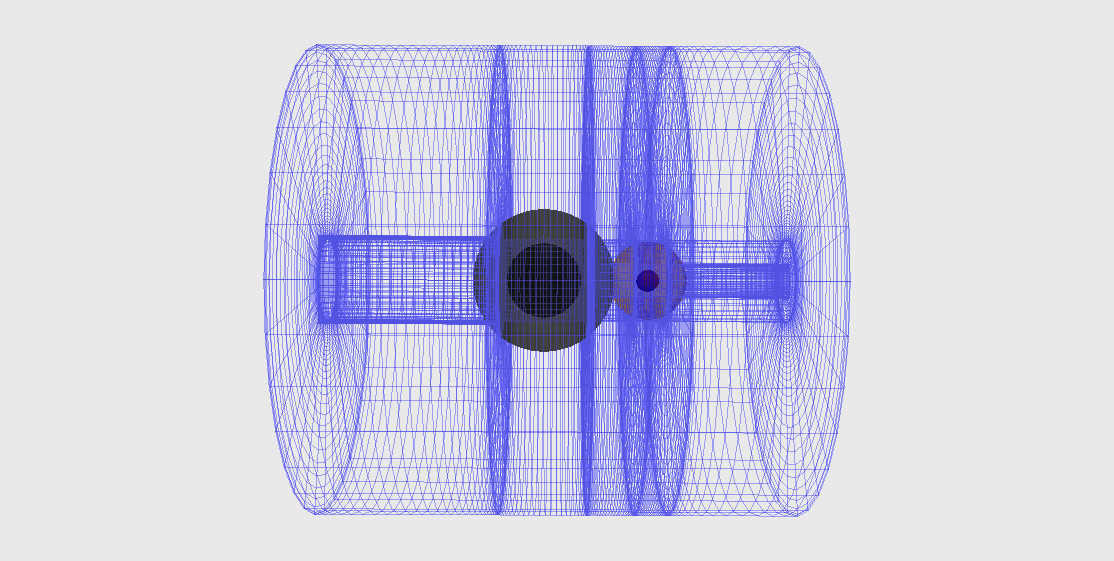
\includegraphics[width=0.8\textwidth]{chap4/BhNsDomain.png}}}
%\caption[Visualization of the BH-NS domain
%decomposition.]{Visualization of the BH-NS domain decomposition. The object on the left is the neutron star, 
%with the colours representing its density. The black object on the right represents the apparent horizon of the black hole. The blue wireframes
%represent the various spheres, cylinders and rectangular parallelepipeds in the domain.
%}
%\label{fig:BHNSDomain}
%\end{figure}

\begin{figure}
\fboxsep0cm  % frame-distance 0
\centerline{\fbox{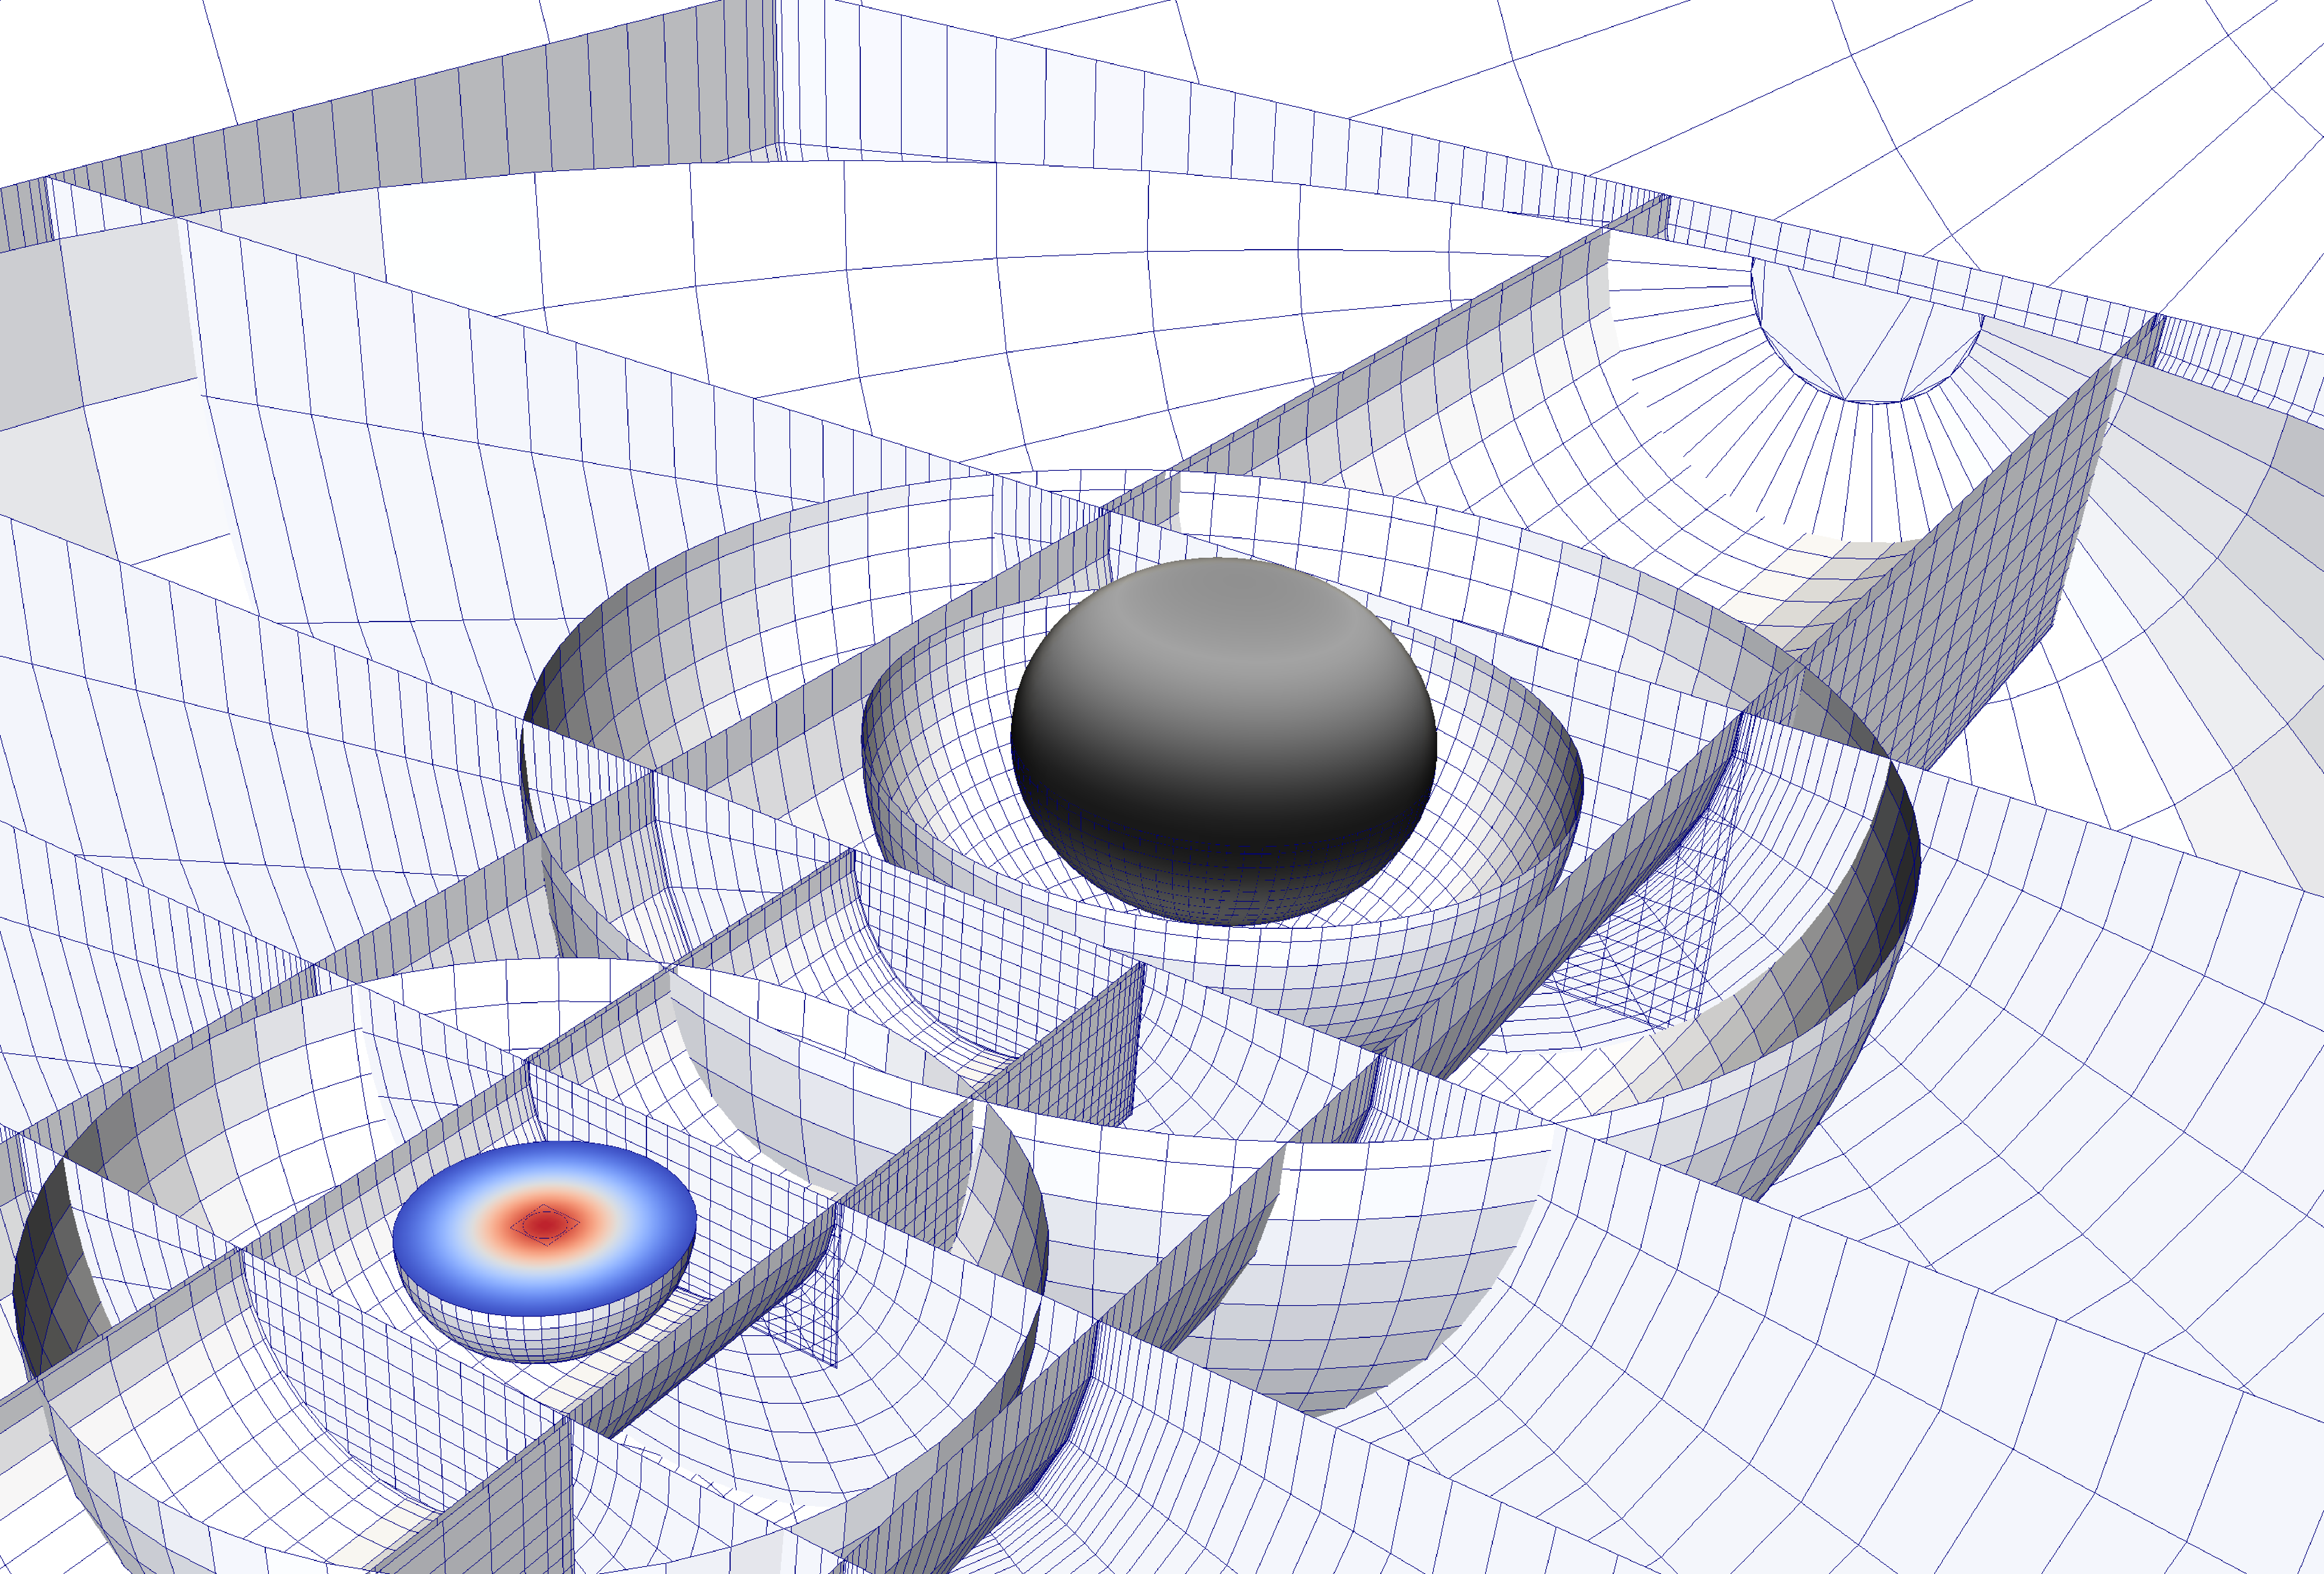
\includegraphics[width=0.8\textwidth]{chap4/BhNsDomain}}}
\caption[Visualization of the BH-NS domain
decomposition.]{Visualization of the BH-NS domain decomposition. The object on the left is the neutron star, 
with the colours representing its density. The black object on the right represents the apparent horizon of the black hole. The blue wireframes
represent the various spheres, cylinders and rectangular parallelepipeds in the domain.


}
\label{fig:BHNSDomain}
\end{figure}

%%%%%%%%%%%%%%%%%%%%%%%%%%%%%%%%%%%%%%%%%%%%%%%%%%%%%%%%%%%%%%%%


The computational domain has the black hole interior excised, and
extends to some large outer boundary ($R=10^{10}$ in practice). To
cover this computational domain with spectral expansions, we split the
domain into multiple subdomains as indicated in
figure~\ref{fig:BHNSDomain}, each one with its own spectral expansion:
The neutron star is covered by a spherical shell with outer boundary
deformed to coincide with the boundary of the neutron star
(cf. Eq.~(\ref{eq:NSSurf}) below). To avoid having to deal with
regularity conditions at the origin, this shell does not cover the
origin; rather a small cube is placed there which overlaps the
spherical shell. The neutron star is surrounded by one further
spherical shell. The black hole is surrounded by two concentric
spherical shells, where the inner boundary of the inner shell
coincides with the apparent horizon, where the boundary
conditions~(\ref{eq:BHBoundary})~--~(\ref{eq:BHBoundary3}) are imposed.
Three rectangular parallelepipeds surround the axis passing through the
centers of the BH and the NS - one between them and one on each side
of the objects. An additional eight cylindrical shells are placed
around the same axis to cover the intermediate field region. The
far-field region is covered by a large spherical shell whose outer
boundary is placed at $R=10^{10}$ using an inverse radial
mapping.

All variables (metric and hydrodynamical) are decomposed on sets of
basis functions on each subdomain. The type of basis function depends
on the topology on the subdomain. Finite difference schemes are needed
for hydrodynamical quantities during evolutions so as to capture
shocks, but for initial data, where shocks are not present, spectral
methods are suitable and exponential convergence can be achieved. The
resolution of each domain is synonymous with the number of colocation
points used. The resolution of each subdomain is initialized manually
at the start of the initial data solve; subsequently, the resolution
is adjusted several times using an adaptive mesh refinement (AMR) scheme (see
step~\ref{it:final}). To discuss the resolution of the computational
domain for the purpose of convergence tests, we denote by $N$
the total number of collocation points in all subdomains. $N^{1/3}$ is then a measure of linear resolution.
A typical initial data solve starts with, $N^{1/3}\sim 33$ and ends
with $N^{1/3}\sim 80$.

\subsection{Diagnostics}


The angular momentum of the black hole is
computed as~\citep{Lovelace2008,FoucartEtAl:2008}
\begin{equation}
\label{eq:BHSpin}
S=\frac{1}{8\pi}\oint_{\mathcal{H}}\phi^is^jK_{ij}dA.
\end{equation}
 In a space-time with aziumuthal symmetry, $\phi^i$ would represent
 the exact azimuthal Killing vector field generated by this symmetry.
Since azimuthal symmetry is not present in a binary system, we
instead use an {\it approximate} Killing vector. It is computed by solving a
shear minimization eigenvalue problem - see
\cite{Cook2007,Lovelace2008}  for details. The dimensionless spin is defined as
\begin{equation}
\label{eq:ChiDef}
\chi=\frac{S}{M^2},
\end{equation}
where $M$ is the Christodoulou mass,
\begin{equation}
M^2=M_{\rm irr}^2+\frac{S^2}{4M_{\rm irr}^2}.
\end{equation}
The irreducible mass is related to the surface area of the apparent horizon, $A$,
\begin{equation}\label{eq:Mirr}
M_{\rm irr}=\sqrt{A/16\pi}.
\end{equation}


We employ similar surface integrals to compute the dimensionless spin
of the neutron star. In particular we use Eq.~\ref{eq:BHSpin}, with
$\mathcal{H}$ replaced by the neutron star's surface, as defined in
Eq.~\ref{eq:NSSurf} to compute the star's angular momentum
$S_{\rm NS}$.

To define the neutron star's mass, we use the Arnowitt-Deser-Misner
(ADM) mass $M_{\rm ADM, NS}$ of an {\it isolated} neutron star with
same rotation. In particular, we use the methods described
in~\cite{cook94a} to solve for the equilibrium state of an
isolated neutron star with the same baryon mass, equation of state,
and angular momentum, as the neutron star in our binary, and then
compute its ADM mass. The dimensionless neutron star spin is 
defined as
\begin{equation}
  \chi_{\rm NS}=\frac{S_{\rm NS}}{M_{\rm ADM, NS}^2}.
\end{equation}
~\cite{Tacik:2015tja} showed that this method of computing
neutron star spin was robust and accurate.


The ADM linear momentum is defined by a surface integral at infinity~\citep{ADM,York:1979},
\begin{equation}\label{eq:PADM}
P_{\rm ADM}^i = \frac{1}{8\pi}\oint_{S_{\infty}}K^{ij}dS_j.
\end{equation}
This integral relies on cancellation of leading order terms~\citep{FoucartEtAl:2008,Ossokine:2015yla}, which
results in loss of accuracy when evaluated at finite numerical
precision. Therefore, we use Gauss' law to rewrite~\citep{FoucartEtAl:2008,Ossokine:2015yla}
equation~(\ref{eq:PADM}) as a surface integral over a sphere with
smaller radius, $\mathcal{S}_0$, and a volume-integral over the volume
$V_0$ outside $\mathcal{S}_0$, 
\begin{equation}\label{eq:PADM2}
P_{\rm ADM}^i = \frac{1}{8\pi}\oint_{S_0}P^{ij}dS_j-\frac{1}{8\pi}\int_{V_0}G^idV,
\end{equation}
where
\begin{eqnarray}
P^{ij}=\Psi^{10}\left(K^{ij}-K\gamma^{ij}\right),\\
G^i=\tilde{\Gamma}^i_{jk}P^{jk}+\tilde{\Gamma}^j_{jk}P^{ik}-2\tilde{\gamma}_{jk}P^{jk}\tilde{\gamma}^{il}\partial_l\left(\log\Psi\right).
\end{eqnarray}


\subsection{Iterative Procedure}

Construction of initial data begins by choosing the physical
parameters of the BH-NS binary, which we aim to achieve.
For the black hole, we specify:
\begin{itemize}
\item The black hole mass, $M_{\rm BH}$,
\item The black hole's dimensionless spin vector,
  $\vec{\chi}_{\rm BH}$.
\end{itemize}
For the neutron star we specify:
\begin{itemize}
\item The neutron star's baryon mass, $M_{b}$,
\item The neutron star's equation of state, 
\item The neutron star's spin vector, $\omega^i$.
\end{itemize}
Finally, characterizing the orbit are:
\begin{itemize}
\item The separation between the centers of the BH and NS, $D$,
\item The orbital angular velocity, $\Omega_0$,
\item The initial infall velocity parameter, $\dot{a}_0$.
\end{itemize}

Additionally, a prescription is required for the free metric
variables, $\tilde{\gamma}_{ij}$ and $K$. Near the black hole, we
would like these variables to approach the spatial metric
$\gamma_{ij}^{\rm KS}$ and mean curvature $K^{\rm KS}$ of a single
rotating black hole in Kerr-Schild coordinates. Away from the black hole (most notably in the vicinity of the neutron star), we desire conformal flatness and maximal slicing. Overall, therefore, we set 
\begin{eqnarray}
  \tilde\gamma_{ij}&=&\delta_{ij} + e^{(-r/w)^4}\left(g_{ij}^{\rm KS} -
  \delta_{ij}\right),\\ K &=& e^{(-r/w)^4} K^{\rm KS},
\end{eqnarray}
where $r$ is the distance to the center of the black hole and $w$ is the
roll-off distance.




Once all physical parameters are specified an iterative procedure is
used to solve the various elliptic equations and additional
conditions, We proceed as follows:
\begin{enumerate}
  \renewcommand{\theenumi}{\arabic{enumi}}
\item Initialize two counters for nested iterative loops, $k=0$ and $n=0$. Here, $k$ represents the AMR resolution iterations, and $n$ represents iterations at constant AMR resolution.
  \item
  \label{it:1}
  If $k=0$, 
  at the first iteration (i.e. step~\ref{it:secondlast} has not been
  reached yet), set $\omega^i=0$. Otherwise set $\omega^i$ to its
  desired value, cf. above. This has been found to improve overall
  convergence, especially for high neutron star spins.
\item 
\label{it:solve}
Solve the non-linear XCTS equations~\ref{eq:XCTS-Shift}--\ref{eq:XCTS-Lapse} for the metric variables
  $\beta^i,\Psi,\alpha\Psi$ assuming the matter source
  terms are fixed. For $n=0$ this defines the metric variables $X^{(0)}$ at the 0-th iteration, where $X$ indicates each of the metric variables.
If $n\ge 1$, update the metric variables using a relaxation
  scheme
\begin{equation}
\label{eq:Relaxation}
X^{(n+1)}=\lambda X^{*} + (1-\lambda)X^{(n)},
\end{equation}
where $X^{*}$ is the
result found by solving the XCTS equations. We use $\lambda=0.3$.

\item If both the NS and BH have either aligned spin or zero spin,
  impose equatorial symmetry. This speeds up convergence and
  decreases computational cost.

\item
  \label{it:toplevelparamsolve}

 If $k\ge 4$ go directly to
  step~\ref{it:omega}. (We generally find that after four
  resolution-updates, the stellar and black hole parameters are
  computed to sufficient accuracy. Skipping
  steps~\ref{it:surface}--\ref{it:OmegaUpdate} decreases computational
  cost.)
\item 
\label{it:surface}
Locate the surface of the star. The surface of the star is
  represented in terms of spherical harmonics
\begin{equation}
\label{eq:NSSurf}
R(\theta,\phi)=\sum_{l=0}^{l_{\rm max}}\sum_{|m|\le l} c_{lm}Y^{lm}(\theta,\phi).
\end{equation}
The coefficients $c_{lm}$ are determined by solving the relation $h\left(R\left(\theta,\phi\right)\right)=1$.
We generally use $l_{\rm max}=11$.

\item Compute the ADM linear momentum $P_{\rm ADM}$ by evaluating Eq.~\ref{eq:PADM}.
If its norm has changed by less than 10\% in the last iteration, move
the center of the BH by an amount $\delta\vec{c}$, designed to zero the in-plane components of $P^i_{\rm ADM}$, by finding $\delta \vec{c}$ such that $\delta\vec{c}
\times \vec{\Omega}_0=\vec{P}_{\rm ADM}$. Additionally, increase the
radius of the excision surface $r_{\rm ex}$ to
drive $M_{\rm BH}$ to the desired value by applying~\citep{Buchman:2012dw}
\begin{equation}
\delta r_{\rm ex} = -r_{\rm ex} \frac{M_{\rm BH} - M_{\rm
    BH}^{*}}{M_{\rm BH}},
\end{equation}
where $M_{\rm BH}$ is the measured value in the initial data solve and
$M_{\rm BH}^{*}$ is the desired value.

\item \label{it:OmegaUpdate} Compute the spin of the BH by evaluating Eq.~\ref{eq:BHSpin}. Then
  modify the vector $\Omega^i_{\rm BH}$ in Eq.~\ref{eq:BHBoundary3} to drive
  the black hole spin to the target value,  by applying~\citep{Buchman:2012dw}
\begin{equation}
\delta \Omega_{\rm BH}^i = -\frac{\chi^i_{\rm BH}-\chi_{\rm
    BH}^{*i}}{4M}+\frac{M_{\rm BH}-M_{\rm BH}^{*}}{4M_{\rm
    BH}^2}\chi_{\rm BH}^i,
\end{equation}
where $\chi^i_{\rm BH}$ is the computed black hole spin, and $\chi_{\rm
    BH}^{*i}$ is the target spin (see also~\citep{Ossokine:2015yla}).

\item
\label{it:omega}
 If desired, adjust the orbital angular frequency using
  Eq.~\ref{eq:OmegaDriver}, which, after expanding the shift as 
$\beta^i=\beta^i_0 +
\vec{\Omega}\times\vec{r} + \dot{a}\vec{r}$, is a second-order
equation for $\Omega$.

\item Fix the Euler constant by evaluating the integral
\begin{equation}
M_{B}=\int \rho_0\Psi^6\gamma_ndV
\end{equation}
as a function of the Euler
constant $C$ (recall that $C$ enters into $h$, cf. Eq.~\ref{eq:hSoln}, and that $\rho_0$, in turn, depends on $h$, cf. Eq.~\ref{eq:hDefn}). With the secant method, find the value of $C$ that yields the desired baryon mass of the neutron star.

\item Solve the elliptic equation~(\ref{eq:Continuity2}) for the velocity potential $\phi$
  and update $\phi$ using the relaxation scheme in Eq.~\ref{eq:Relaxation}.
  
\item
\label{it:secondlast}
Check whether the Euler constant, black hole mass, black hole spin, ADM linear momentum, and the constraints 
are satisfied to the desired accuracy. If so, proceed to step~\ref{it:final}. Otherwise increment $n$ and return to step~\ref{it:solve}.

\item 
\label{it:final}
Compute the truncation error for the current solution by examining the
spectral coefficients of the metric variables~\citep{Szilagyi:2014fna}.
If the truncation error is too large (generally we use $10^{-9}$ as
the criterion), adjust the number of grid points. Then increment $k$, set $n=0$, and return to
step~\ref{it:1}. This adaptive refinement is based on the target
truncation error and the measured convergence rate of the
solution. See~\cite{Szilagyi:2014fna} for a complete description of
this procedure.

\end{enumerate}

\section{Results}
\label{sec:BHNSResults}




%%%%%%%%%%%%%%%%%%%%%%%%%%%%%%%%%%%%%%%%%%%%%%%%%%%%%%%%%%%%%%%%
\subsection{Initial Data Set Parameters}
%%%%%%%%%%%%%%%%%%%%%%%%%%%%%%%%%%%%%%%%%%%%%%%%%%%%%%%%%%%%%%%%


Our primary goal is to establish the performance of the initial data
solver described in Sec.~\ref{sec:BHNSNumMethods}. The parameter
space of BH-NS binaries is large, encompassing the masses of black
hole and neutron star, their spin magnitudes and their spin
directions, as well as the compactness of the neutron star. As our
first stage in exploring this parameter space, we add neutron star
spin to BH-NS initial data sets that already appeared in the
literature before (namely in~\cite{Foucart:2013a}). Our basis is six BH-NS configurations with
different compactnesses  of the neutron star, and with different
orientations of the black hole spin relative to
the orbital angular momentum. All base-configurations have mass ratio
$q=7$,
black hole spin magnitude of $\chi_{\rm BH}=0.9$ and
neutron star mass of
$M^{\rm NS}_{\rm ADM}=1.4M_{\odot}$ (recall that $M^{\rm NS}_{\rm ADM}$ is the mass of an individual neutron star of the same properties). 

We explore three polytropic equations of state, $P=\kappa\rho^\Gamma$, all with
$\Gamma=2$. $\kappa$ is chosen to achieve neutron star compactnesses
$C=R/M=0.170, 0.156$, $0.144$, and radii of approximately
$12{\rm km}$, $13{\rm km}$, $14{\rm km}$, respectively, for
non-spinning neutron stars with ADM Mass $1.4M_{\odot}$. 

For all three equations of state, we consider BH spin-direction
parallel to the orbital angular momentum. For the stiffest equation
of state, we also vary the BH-spin direction and compute initial data
sets for misalignment angles $\iota=20^{\circ}, 40^{\circ},$ and
$60^{\circ}$. The base-configurations are named {\tt R}xx{\tt i}yy,
where 'xx' denotes the approximate NS radius in kilometers and 'yy' denotes
the inclination between BH spin direction and the orbital angular
momentum in degrees (for instance {\tt R14i20}).

%%%%%%%%%%%%%%%%%%%%%%%%%%%%%%%%%%%%%%%%%%%%%%%%%%%%%%%%%%%%%%%%
\begin{longtable}{l|c|c|c|c|c}
\centering
\label{tab:36sets}
Name & $\Theta_{\rm BH}$ & $M^B_{\rm NS}$ & $M\Omega_{0}$ & {$\vec{\omega}_{\rm NS}$} & $\chi_{\rm NS}$ 
\\
\hline
%\mr
{\tt R12i0$\uparrow$}&$0^\circ$ & 1.5212 & 0.0413  & 0.00667{$\hat{z}$}\hfill & 0.0995 \\
{\tt R12i0$\Uparrow$}&$0^\circ$ & 1.5212 & 0.0413  & 0.0225$\hat{z}$ & 0.4093 \\
{\tt R12i0$\downarrow$}&$0^\circ$ & 1.5212 & 0.0413  & -0.00667$\hat{z}$& -0.0895\\
{\tt R12i0$\Downarrow$}&$0^\circ$ & 1.5212 & 0.0413  & -0.0225$\hat{z}$ & -0.4030 \\
{\tt R12i0$\rightarrow$}&$0^\circ$ & 1.5212 & 0.0413  & 0.00667$\hat{x}$ & 0.0936\\
{\tt R12i0$\Rightarrow$}&$0^\circ$ & 1.5212 & 0.0413  & 0.0225$\hat{x}$ & 0.3989 \\
\hline
{\tt R13i0$\uparrow$}&$0^\circ$ & 1.5128 & 0.0413   & 0.00555$\hat{z}$ & 0.0997 \\
{\tt R13i0$\Uparrow$}&$0^\circ$ & 1.5128 & 0.0413  & 0.019$\hat{z}$ & 0.3911 \\
{\tt R13i0$\downarrow$}&$0^\circ$ & 1.5128 & 0.0413  & -0.00555$\hat{z}$ & -0.0845\\
{\tt R13i0$\Downarrow$}&$0^\circ$ & 1.5128 & 0.0413  & -0.019$\hat{z}$ & -0.3793 \\
{\tt R13i0$\rightarrow$}&$0^\circ$ & 1.5128 & 0.0413 &  0.00555$\hat{x}$ & 0.0913\\
{\tt R13i0$\Rightarrow$}&$0^\circ$ & 1.5128 & 0.0413  & 0.019$\hat{x}$ & 0.3771 \\
\hline
{\tt R14i0$\uparrow$}&$0^\circ$ & 1.5049 & 0.0413 &  0.005541$\hat{z}$ & 0.1188\\
{\tt R14i0$\Uparrow$}&$0^\circ$ & 1.5049 & 0.0413 &  0.017$\hat{z}$ & 0.4109\\
{\tt R14i0$\downarrow$}&$0^\circ$ & 1.5049 & 0.0413 & -0.005541$\hat{z}$& -0.0965\\
{\tt R14i0$\Downarrow$}&$0^\circ$ & 1.5049 & 0.0413  & -0.017$\hat{z}$ & -0.3915\\
{\tt R14i0$\rightarrow$}&$0^\circ$ & 1.5049 & 0.0413  & 0.005541$\hat{x}$ & 0.1066\\
{\tt R14i0$\Rightarrow$}&$0^\circ$ & 1.5049 & 0.0413  & 0.017$\hat{x}$ & 0.3907\\
\hline
{\tt R14i20$\uparrow$}&$20^\circ$ & 1.5049 & 0.0412  & 0.005541$\hat{z}$ & 0.1188 \\
{\tt R14i20$\Uparrow$}&$20^\circ$ & 1.5049 & 0.0412  & 0.017$\hat{z}$ & 0.4110\\
{\tt R14i20$\downarrow$}&$20^\circ$ & 1.5049 & 0.0412  &  -0.005541$\hat{z}$& -0.0964\\
{\tt R14i20$\Downarrow$}&$20^\circ$ & 1.5049 & 0.0412  & -0.017$\hat{z}$ & -0.3915\\
{\tt R14i20$\rightarrow$}&$20^\circ$ & 1.5049 & 0.0412  & 0.005541$\hat{x}$ & 0.1064\\
{\tt R14i20$\Rightarrow$}&$20^\circ$ & 1.5049 & 0.0412  & 0.017$\hat{x}$ & 0.3905 \\
\hline
{\tt R14i40$\uparrow$}&$40^\circ$ & 1.5049 & 0.0412  &  0.005541$\hat{z}$ & 0.1193 \\
{\tt R14i40$\Uparrow$}&$40^\circ$ & 1.5049 & 0.0412  & 0.017$\hat{z}$ & 0.4117\\
{\tt R14i40$\downarrow$}&$40^\circ$ & 1.5049 & 0.0412  & -0.005541$\hat{z}$& -0.0961\\
{\tt R14i40$\Downarrow$}&$40^\circ$ & 1.5049 & 0.0412  & -0.017$\hat{z}$ & -0.3908\\
{\tt R14i40$\rightarrow$}&$40^\circ$ & 1.5049 & 0.0412 & 0.005541$\hat{x}$ & 0.1064\\
{\tt R14i40$\Rightarrow$}&$40^\circ$ & 1.5049 & 0.0412  & 0.017$\hat{x}$ & 0.3905 \\
\hline
{\tt R14i60$\uparrow$}&$60^\circ$ & 1.5049 & 0.0415  &  0.005541$\hat{z}$ & 0.1200 \\
{\tt R14i60$\Uparrow$}&$60^\circ$ & 1.5049 & 0.0415  & 0.017$\hat{z}$ & 0.4132\\
{\tt R14i60$\downarrow$}&$60^\circ$ & 1.5049 & 0.0415  & -0.005541$\hat{z}$& -0.0954\\
{\tt R14i60$\Downarrow$}&$60^\circ$ & 1.5049 & 0.0415 & -0.017$\hat{z}$ & -0.3898\\
{\tt R14i60$\rightarrow$}&$60^\circ$ & 1.5049 & 0.0415 & 0.005541$\hat{x}$ & 0.1061\\
{\tt R14i60$\Rightarrow$}&$60^\circ$ & 1.5049 & 0.0415 & 0.017$\hat{x}$ & 0.3903\\
\hline
\caption[Initial data set parameters for series of 36 BH-NS initial
data sets.]{\label{tab:36Sets} Full set of parameters of
 the 36 sets of initial data constructed here. Given are 
 angle between the black hole spin and the orbital angular
  momentum $\theta_{\rm BH}$, baryon mass of the neutron star  $M^B_{\rm NS}$, orbital frequency $M\Omega_0$, spin vector $\vec{\omega}_{\rm NS}$ of the neutron star (cf. Eq.~\ref{eq:RotationTerm}), and the dimensionless spin of the neutron star, $\vec{\chi}_{\rm NS}$.}
\end{longtable}
%%%%%%%%%%%%%%%%%%%%%%%%%%%%%%%%%%%%%%%%%%%%%%%%%%%%%%%%%%%%%%%%

For the base-configurations, the following secondary choices are made:
The non-parallel part of the black hole spin is set parallel
to the $\hat{x}$ axis, i.e., the approximate axis between the BH and the NS. In each case the initial separation between the
black hole and the neutron star is $D=7.44M$, where
$M=M_{\rm BH}+M^{\rm ADM}_{\rm NS}$ is the total mass of the
binary. The initial infall velocity parameter $\dot{a}_0$ is set to
$0$. The orbital angular velocity, $\Omega_0$, is the same as in
~\cite{Foucart:2013a} and is indicated in
table~\ref{tab:36Sets}. The above constitutes 6 different
configurations.

We combine each of the six base-configurations with six different
configurations of neutron star spins for a total of 36 total
configurations. In particular we choose three directions - aligned
with the orbital angular momentum, anti-aligned with the orbital
angular momentum, and parallel to the orbital plane (along the
$+\hat{x}$ direction). For each of these three $\hat\chi_{\rm NS}$ directions, we consider
``large'' and ``small'' neutron star spin magnitude,
$\chi_{\rm NS}\sim 0.4$ and $\chi_{\rm NS}\sim 0.1$. In our
naming notation, we use a double arrow ($\Uparrow$) for the
large $\chi_{\rm NS}$ configurations and a single arrow ($\uparrow$) for the
small $\chi_{\rm NS}$ configurations, with the direction of the arrow indicating the direction
of the NS spin vector (e.g. {\tt R14i20}$\rightarrow$). The full parameters of the initial data sets
are summarized in Table ~\ref{tab:36Sets}. 



In the present chapter, we do not perform evolutions of these initial
data sets. Based on the evolutions in~\cite{Foucart:2013a} (for
non-spinning NS), we expect these initial data sets to correspond to
binaries that will proceed through $\sim 7$ to $\sim 10$ orbits before
merger.



%%%%%%%%%%%%%%%%%%%%%%%%%%%%%%%%%%%%%%%%%%%%%%%%%%%%%%%%%%%%%%%%
\subsection{Convergence of the Initial Data Solver}
\label{sec:Convergence}
%%%%%%%%%%%%%%%%%%%%%%%%%%%%%%%%%%%%%%%%%%%%%%%%%%%%%%%%%%%%%%%%

To assess the convergence of the initial data solver we will begin by looking at the convergence of the iterative part of the solver. That is, the convergence of steps 1-12 in the iterative procedure
described above. We will first focus on one particular initial data
set of the 36 in Tab~\ref{tab:36Sets} - namely the {\tt
  R14i60$\Uparrow$} initial data set. The results we present for {\tt
  R14i60$\Uparrow$}, however, are representative for all of the 36 sets considered.

%%%%%%%%%%%%%%%%%%%%%%%%%%%%%%%%%%%%%%%%%%%%%%%%%%%%%%%%%%%%%%%%
\setcounter{figure}{1}
\begin{figure}
\centerline{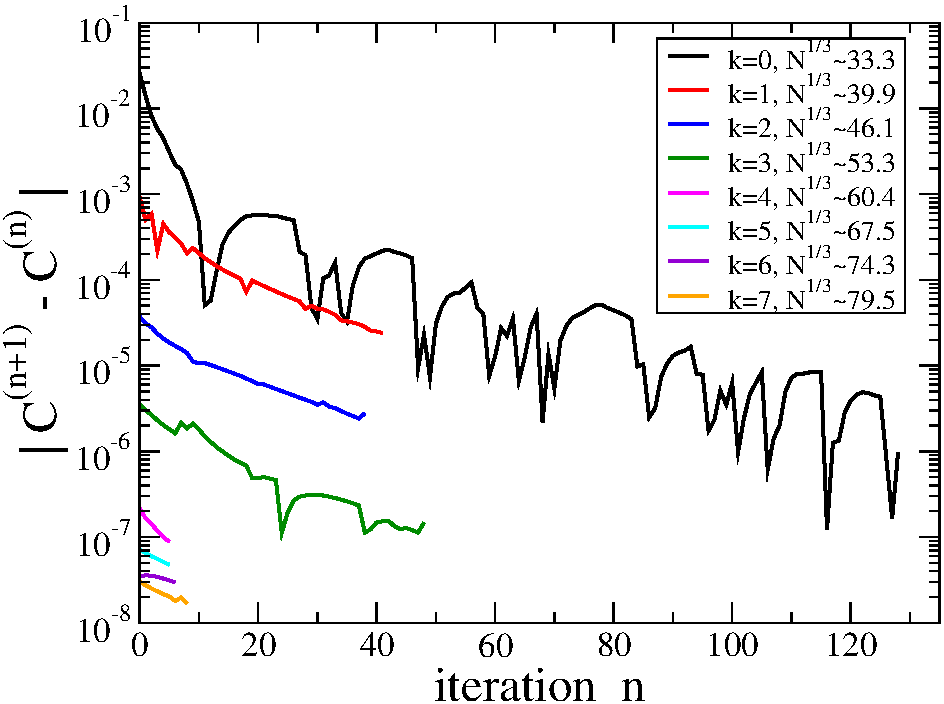
\includegraphics[scale=0.95]{chap4/EulerConv}}
\caption[Convergence of the Euler constant.]{\label{Fig:EulerConv}
Absolute difference between neighbouring iterations of the Euler
constant for the {\tt R14i60$\Uparrow$} initial data set. $k$ labels AMR adjustment iterations, and $n$ the inner iterative loop at fixed grid-resolution.}
\end{figure}
%%%%%%%%%%%%%%%%%%%%%%%%%%%%%%%%%%%%%%%%%%%%%%%%%%%%%%%%%%%%%%%%

We begin by looking at the convergence of the Euler constant, $C$. In figure~\ref{Fig:EulerConv} we plot the absolute difference in $C$ between neighbouring iterations for the eight
different resolutions used in the initial data solve. 
In the figure we see that at a given resolution these differences
decrease exponentially with iteration as expected for the relaxation
scheme employed (cf. Eq.~\ref{eq:Relaxation}). Meanwhile the differences also decrease with increasing resolution. 
We find similar results for all the other initial data sets we
consider.

%%%%%%%%%%%%%%%%%%%%%%%%%%%%%%%%%%%%%%%%%%%%%%%%%%%%%%%%%%%%%%%%
\begin{figure}
  \centerline{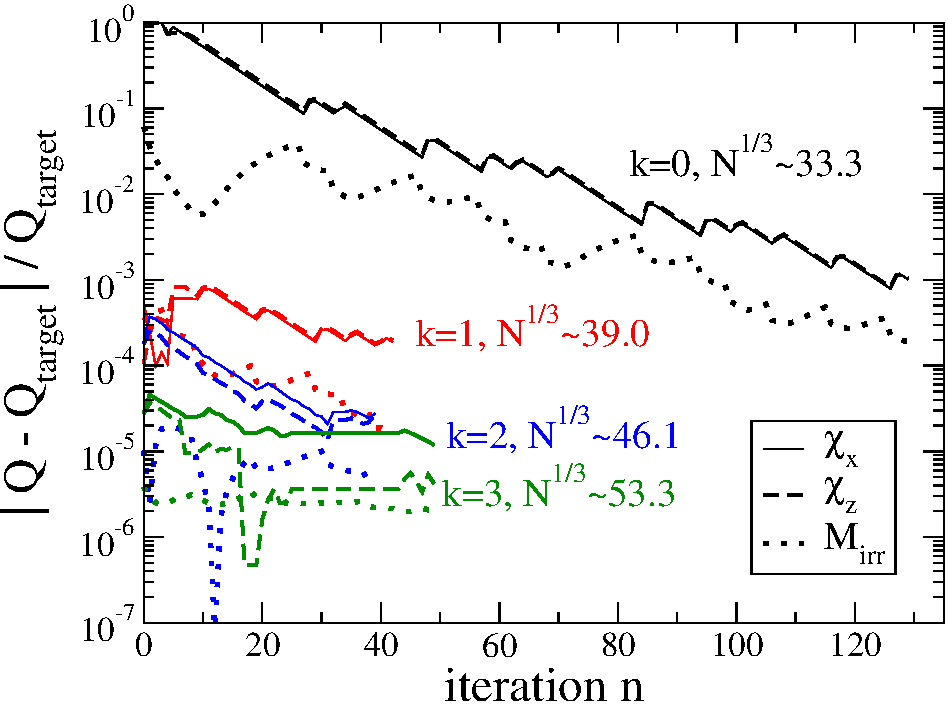
\includegraphics[scale=0.95]{chap4/BHSpinConv}}
\caption[Convergence of black hole spin and mass.]
{\label{Fig:BHSpinConv}Fractional difference from desired values of
  black hole spin and mass. Shown is the solution of {\tt
    R14i60$\Uparrow$} initial data set as a function of iteration
  count. The four colours represent the four different resolutions
  $k=0,\ldots,3$ at which the black hole spin is measured. }
\end{figure}
%%%%%%%%%%%%%%%%%%%%%%%%%%%%%%%%%%%%%%%%%%%%%%%%%%%%%%%%%%%%%%%%

Next, we will look at the properties of the black hole to verify that
they converge as expected in the presence of a spinning neutron star,
using again {\tt R14i60$\Uparrow$} as our example. We focus on the
black hole spin $\vec\chi_{\rm BH}$ which is controlled by the
parameter $\Omega_j^{\rm BH}$ in Eq.~\ref{eq:BHBoundary3}, and the
irreducible black hole mass, $M_{\rm irr}$ (cf. Eq.~\ref{eq:Mirr}).

Figure~\ref{Fig:BHSpinConv} shows the fractional difference for these quantities to their desired target value.
 The
difference is plotted as a funciton of iteration, for four different
resolutions. Recall that the BH spin is only adjusted on iterations $k=0,1,2,3$, and not thereafter (cf. Step~\ref{it:toplevelparamsolve}). In general we see a decrease in this difference with iteration, especially at the first resolution, therefore showing that the iterative solver is correctly driving the the black hole properties to the target values.
Furthermore, that this difference decreases with resolution, and
we are able to achieve an accuracy of about $10^{-5}$ in the BH spin
and mass. Note that these differences continue to remain small for $k>3$.

Having established the convergence of the iterative procedure, we
turn now to the global
properties of the solution, continuing to focus on the {\tt R14i60$\Uparrow$} ID set. We first consider the Hamiltonian and momentum constraints, computed as
\begin{eqnarray}
H&=||\frac{R_{\Psi}}{8\Psi^5}||,\\
M &= ||\frac{R_{\beta}}{2\alpha\Psi^4}||,
\end{eqnarray}
where $R_{\Psi}$ and $R_{\beta}$ are the residuals of
Eqs.~\ref{eq:XCTS-ConformalFactor} and~\ref{eq:XCTS-Shift},
respectively, and $||.||$ represents the $L2$ norm over all
collocation points of the computational domain. The constraints for
this ID set are shown in figure~\ref{fig:HamMom}. We find exponential
convergence in the constraints, as expected for spectral methods. 
The increase at the second iteration ($k=1$) arises because the
neutron star spin is only activated in the second iteration 
(cf. step~\ref{it:1}).

%%%%%%%%%%%%%%%%%%%%%%%%%%%%%%%%%%%%%%%%%%%%%%%%%%%%%%%%%%%%%%%%
\begin{figure}
\centerline{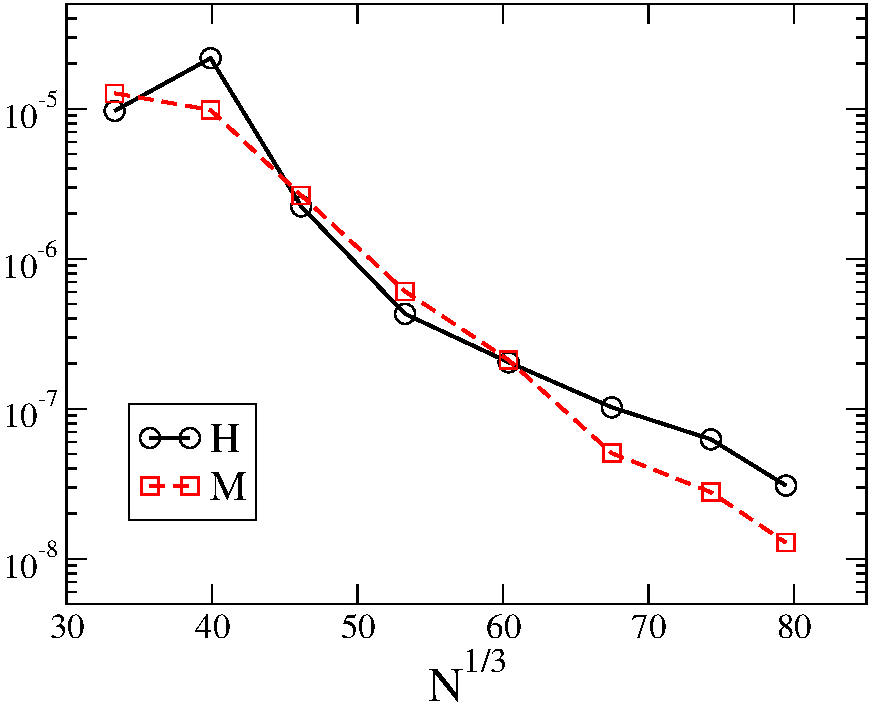
\includegraphics[scale=0.95]{chap4/HamMom}
}
\caption[Hamiltonian and momentum constraints of the {\tt R14i60$\Uparrow$} ID set]{\label{fig:HamMom} The Hamiltonian and momentum constraints for the {\tt R14i60$\Uparrow$} initial data set
as a function of resolution. We find exponential convergence in both.}
\end{figure}
%%%%%%%%%%%%%%%%%%%%%%%%%%%%%%%%%%%%%%%%%%%%%%%%%%%%%%%%%%%%%%%%

Finally, we look at the properties of the neutron star. As noted in Eq.~\ref{eq:NSSurf},
the neutron star surface is expressed as a sum of spherical
harmonics.
To evaluate the convergence of the surface location, we define the
quantity
\begin{equation}
\label{eq:NSSurf2}
\Delta c^{(k)}=\sqrt{\sum_{l,m}
\left(c_{lm}^{(k)}-c^{(k_{\rm max})}_{lm}\right)^2},
\end{equation}
where $k$ represents the current resolution, and $k_{\rm max}$ represents the
highest resolution. This quantity is plotted in
figure~\ref{fig:SpinDiff}. Similar to the black hole surface, the
neutron star surface is only computed for the first four resolutions,
and so we have three data points shown. We find exponential
convergence in this quantity. We also look at the convergence of the
neutron star spin $\chi_{\rm NS}$ measured at each resolution. In
figure~\ref{fig:SpinDiff}, we plot the fractional difference in
$\chi_{\rm NS}$ between neighbouring resolutions. That is, we plot
\begin{equation}\label{eq:NSspin2}
\delta\chi^{(k)}_{\rm NS}=\frac{\big| \chi^{(k+1)}_{\rm NS}-\chi^{(k)}_{\rm NS} \big|}{\chi^{(k)}_{\rm NS}}.
\end{equation}
Figure~\ref{fig:SpinDiff} exhibits exponential convergence, although
there are two disinctly different slopes in the data, once we cease to
update the NS surface for $k\ge 4$. Nevertheless, we are able to
measure the spin to an accuracy of about $10^{-6}$. We have omitted
the first data point of $\delta\chi^{(k)}_{\rm NS}$, because the 
NS spin is not activated for $k=0$ (cf. Step.~ \ref{it:1}).


%%%%%%%%%%%%%%%%%%%%%%%%%%%%%%%%%%%%%%%%%%%%%%%%%%%%%%%%%%%%%%%%
\begin{figure}
\centerline{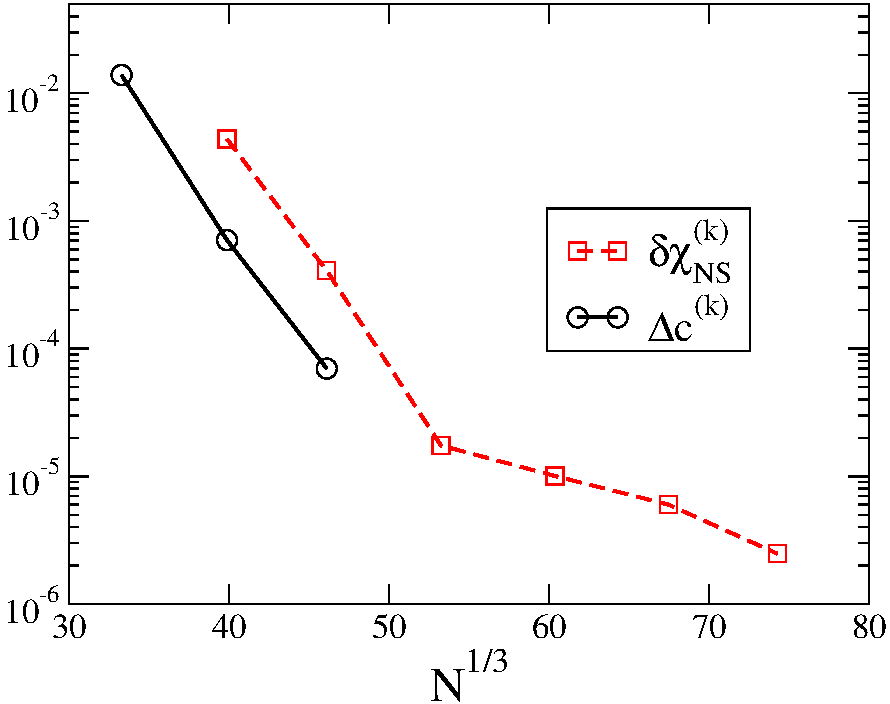
\includegraphics[scale=0.95]{chap4/SpinDiff}}
\caption[Neutron star surface and spin accuracy.]{\label{fig:SpinDiff}
  Accuracy of neutron star properties for the solution of {\tt R14i60$\Uparrow$}. Plotted are the accuracy of the
  NS surface, $\Delta c^{(k)}$, as defined in Eq.~\ref{eq:NSSurf2} and
  the fractional accuracy of the NS spin (equation~\ref{eq:NSspin2}).
}
\end{figure}
%%%%%%%%%%%%%%%%%%%%%%%%%%%%%%%%%%%%%%%%%%%%%%%%%%%%%%%%%%%%%%%%

The above data all show that we have established the convergence of
our initial data solver, by showing exponential convergence of the
iterative solver, the black hole properties, neutron star properties,
and the constraints.

%%%%%%%%%%%%%%%%%%%%%%%%%%%%%%%%%%%%%%%%%%%%%%%%%%%%%%%%%%%%%%%%
\subsection{Broader Exploration of Parameter Space}
\label{sec:MoreParameters}
%%%%%%%%%%%%%%%%%%%%%%%%%%%%%%%%%%%%%%%%%%%%%%%%%%%%%%%%%%%%%%%%


All initial-data sets constructed so far share the same black hole
mass and black hole spin-magnitude, $M_{\rm BH}=9.8_\odot$
and $\chi_{\rm BH}=0.9$. In this section, we relax these
restrictions, and also explore the range of possible neutron star
spins our code is capable to construct. In total, we consider three additional sequences of initial-data sets:

%%%%%%%%%%%%%%%%%%%%%%%%%%%%%%%%%%%%%%%%%%%%%%%%%%%%%%%%%%%%%%%%
\begin{figure}
  %\centerline{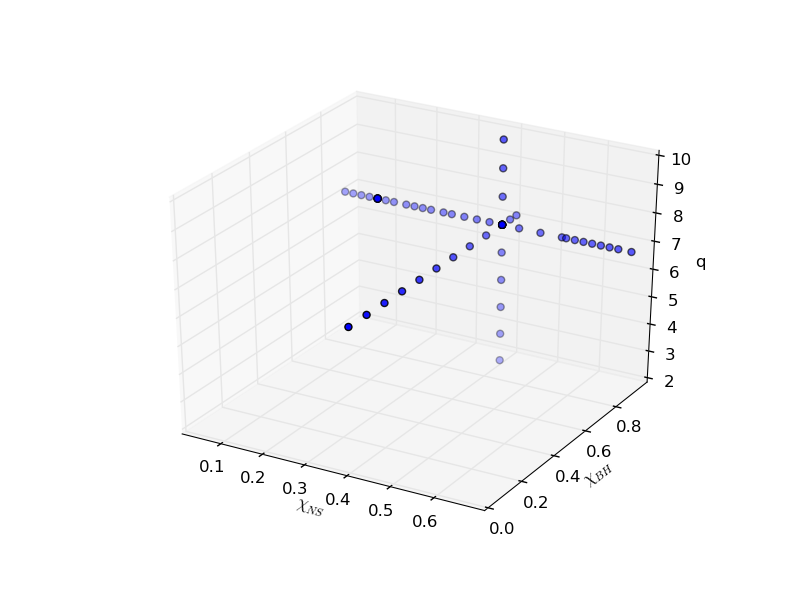
\includegraphics[width=0.95\columnwidth,clip=true, trim=90
    %47 60 68]{chap4/3dparam.png} }
\centerline{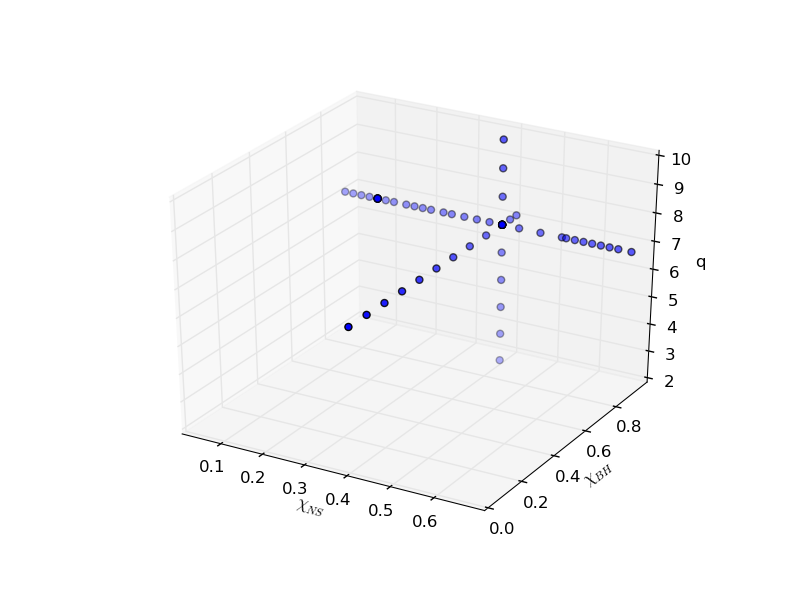
\includegraphics[width=0.95\columnwidth]{chap4/3dparam.png}}
\caption[3d parameter space plot of BH-NS initial data
  sets.]{\label{fig:3dparam} Parameter space exploration. Starting
  from {\tt R14i0$\Uparrow$}(large red circle) we vary (i) the BH
  spin $\chi_{\rm BH}$, (ii) the NS spin $\chi_{\rm NS}$ and (iii) the
  black hole mass $M_{\rm BH}$, indicated by the mass-ratio $q$.}
\end{figure}
%%%%%%%%%%%%%%%%%%%%%%%%%%%%%%%%%%%%%%%%%%%%%%%%%%%%%%%%%%%%%%%%


%%%%%%%%%%%%%%%%%%%%%%%%%%%%%%%%%%%%%%%%%%%%%%%%%%%%%%%%%%%%%%%%
\begin{figure}
\centerline{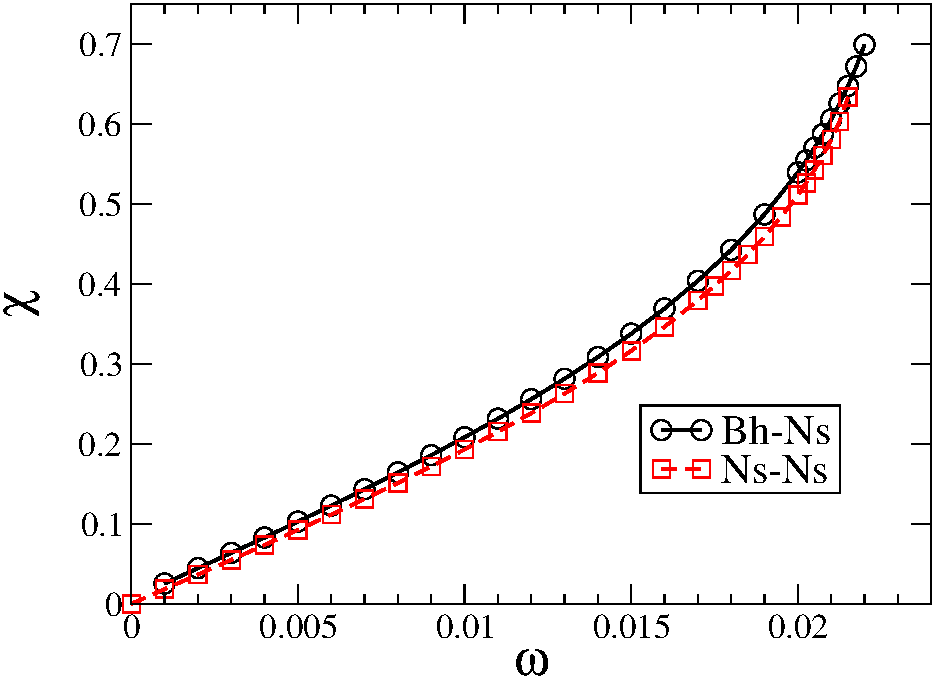
\includegraphics[scale=0.95]{chap4/chiVOmega}}
\caption[$\chi_{\rm NS}$ as a function of $\omega_{\rm NS}$ for bh-ns
binaries]
{\label{fig:ChiVOmega}
Neutron star spin $\chi$ as a function of neutron star spin parameter
$\omega$ for a sequence of initial data sets. The black hole spin is
constant at $\chi=0.9$ and the mass ratio is $q=7$. The dashed red curve is
from NS-NS binaries, with somewhat different neutron star parameters.}
\end{figure}
%%%%%%%%%%%%%%%%%%%%%%%%%%%%%%%%%%%%%%%%%%%%%%%%%%%%%%%%%%%%%%%%

First, we consider a
sequence that varies the neutron star spin from $\chi_{\rm NS}=0$ to
$\chi_{\rm NS}\sim0.7$, keeping it aligned with the orbital angular
momentum. In these initial data sets, the other binary parameters are
the same as in the {\tt R14i0} runs. Namely, the neutron star mass,
equation of state, black hole mass, black hole spin, initial
separation and orbital angular frequency. Second, we consider a
sequence of runs where we vary the black hole spin from $\chi_{\rm
  BH}=0$ to $\chi_{\rm BH}=0.99$, while keeping the other binary
parameters as in the {\tt R14i0$\Uparrow$} run. Finally, we consider
a sequence of runs where we vary the mass ratio from $q=2$ to $q=10$.
Figure~\ref{fig:3dparam} summarizes all the initial data sets along
the axes of $\chi_{\rm NS}$, $\chi_{\rm BH}$ and $q$.


%%%%%%%%%%%%%%%%%%%%%%%%%%%%%%%%%%%%%%%%%%%%%%%%%%%%%%%%%%%%%%%%
\begin{figure}
\centerline{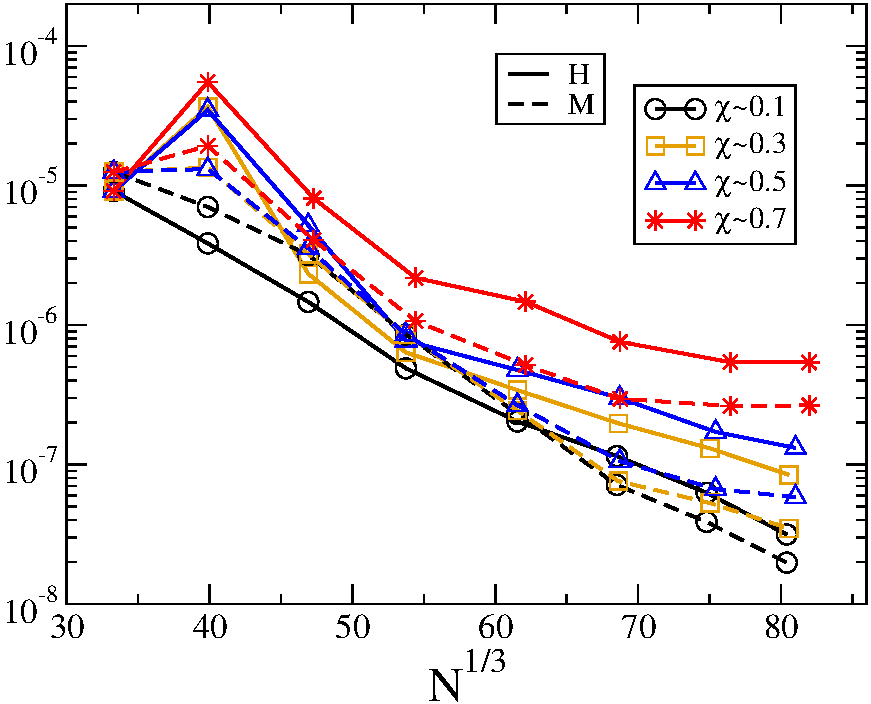
\includegraphics[scale=0.95]{chap4/OmegaSeqHamMom}}
\caption[Constraints for the $\chi_{\rm NS}$ sequence.]{\label{fig:OmegaSeqHamMom} Hamiltonian (solid curves) and
momentum (dotted curves) constraints for four different neutron star spins.}
\end{figure}
%%%%%%%%%%%%%%%%%%%%%%%%%%%%%%%%%%%%%%%%%%%%%%%%%%%%%%%%%%%%%%%%

We begin by varying the neutron star rotation parameter $\omega$. The
parameters in this sequence are otherwise the same as in the {\tt
  R14i0} data sets, and the neutron star spin is kept aligned with the
orbital angular momentum. In Fig.~\ref{fig:ChiVOmega} we plot the
measured neutron star spin $\chi_{\rm NS}$ as a function of the code
parameter $\omega$ for the full sequence. As expected, we find a
linear relationship at low $\omega$, but the relationship becomes
non-linear at higher $\omega$, as the neutron star's size, and thus
moment of inertia, becomes an appreciable function of spin. We find
that the solver breaks down around $\chi_{\rm NS}\sim 0.7$, which is the
maximum spin parameter for neutron stars found in~\cite{Lo:2010bj}. Figure~\ref{fig:ChiVOmega} also shows the
corresponding $\chi_{\rm NS}$ vs. $\omega$ curve for a binary neutron
star of mass-ratio $q=1$ with both stars carrying the same aligned
spin magnitude as presented in~\cite{Tacik:2015tja}. The NS-NS data
use different NS parameters, with mass $M_{\rm ADM}=1.64M_{\odot}$ and
equation of state parameter $\kappa=123.6$. Nevertheless, the curves
remain very close to each other in shape, indicating that the method
to impart NS rotation~\citep{Tichy:2011gw} performs similarly for mixed
BH-NS binaries and for NS-NS binaries~\citep{Tacik:2015tja}.


To investigate numerical convergence of the initial-data sets
presented in figure~\ref{fig:ChiVOmega}, we plot in
figure~\ref{fig:OmegaSeqHamMom} the Hamiltonian and momentum
constraints for a subset of the generated initial data sets, with
$\chi\sim{0.1,0.3,0.5,0.7}$. In general we find the expected
exponential convergence, but there are a few features worth discussing
in the data. The increase in the constraints between the lowest and
second-lowest resolution ($k=0$ vs. $k=1$) arises because the spin is
only activated at the second-lowest resolution, cf. step~\ref{it:1}.
This jump in constraints  monotonically increases with the spin-parameter $\omega$, as we might expect, because the solver has a more difficult task
in adjusting to the abrupt activation of a larger spin. We also note that
at high resolution, in the $\chi\sim 0.7$ curve, we lose exponential
convergence and the curves flatten out around $10^{-6}$. 
This is likely a sign that
the accuracy of the solver is becoming limited, likely by
approximations that go into the solver. $\chi\sim 0.7$ is around the
maximum theoretical neutron star spin, so such difficulties are
expected.


Continuing the exploration of parameter space, we next vary the black
hole spin $\chi_{\rm BH}$. In partiuclar, we vary the black hole spin
from $\chi_{\rm BH}=0$ to $\chi_{\rm BH}=0.99$, keeping it aligned
with the orbital angular momentum. The other binary parameters are
kept the same as in the ${\tt R14i0\Uparrow}$ initial data set,
specifically $\vec{\omega}_{\rm NS}=0.017\hat z$ and $q=7$. In
Figs.~\ref{fig:chiSeqHam} we plot the Hamiltonian and momentum
constraints, respectively, for this sequence. We find exponential
convergence in all cases. It is interesting to note that the
constraints seem to be lowest at the highest black hole spins,
$\chi_{\rm BH}=0.95$ and $\chi_{\rm BH}=0.99$, while one might expect
these to be the most challenging cases.

%%%%%%%%%%%%%%%%%%%%%%%%%%%%%%%%%%%%%%%%%%%%%%%%%%%%%%%%%%%%%%%%
\begin{figure}
\centerline{\hspace*{1.4cm}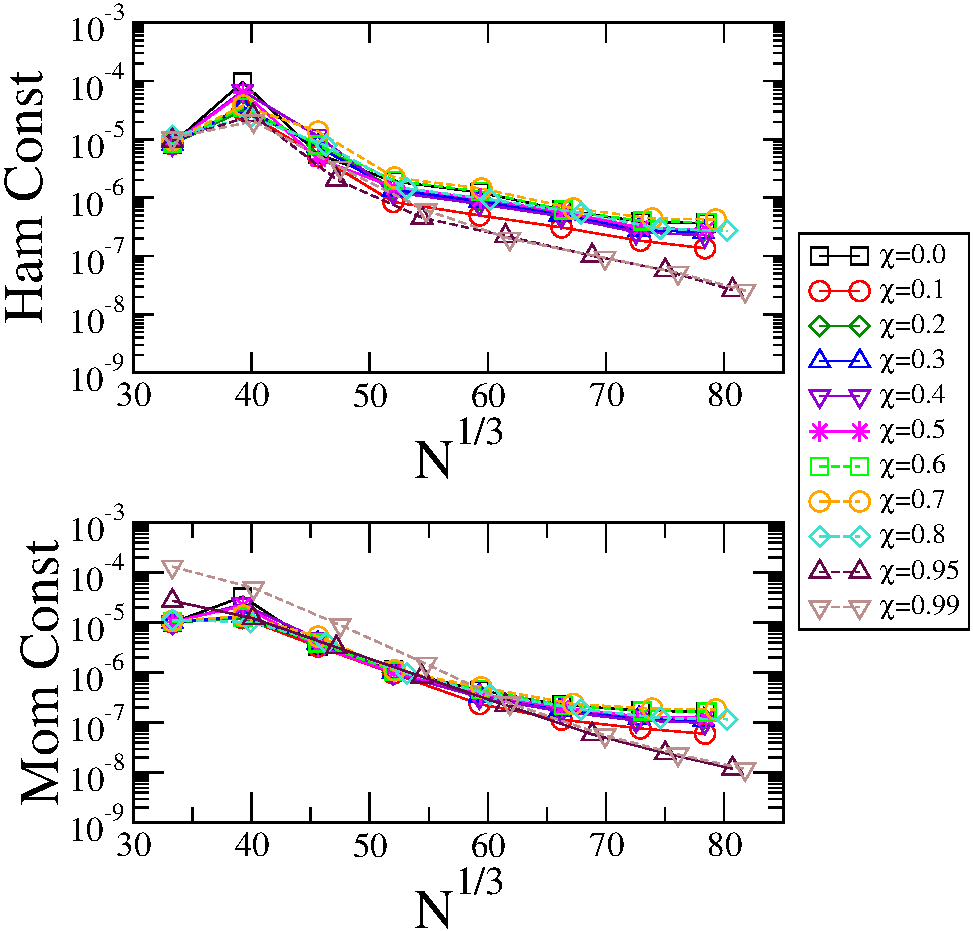
\includegraphics[scale=0.95]{chap4/chiSeqHam}}
\caption[Hamiltonian and momentum constraints for the sequence in $\chi_{\rm
    BH}$.]{\label{fig:chiSeqHam}Hamiltonian constraint (top panel) and momentum
  constraint (bottom panel) versus resolution for our sequence of
  binaries where the black-hole spin is varied from $\chi_{\rm BH}=0$
  to $\chi_{\rm BH}=0.99$. The NS spin parameter is kept constant at $\vec\omega_{\rm NS}=0.017\hat z$ and the mass ratio is $q=7$. 

}
\end{figure}
%%%%%%%%%%%%%%%%%%%%%%%%%%%%%%%%%%%%%%%%%%%%%%%%%%%%%%%%%%%%%%%%

Since this work focuses on neutron star spin, it is interesting to
consider how the measured neutron star spin, $\chi_{\rm NS}$ couples
to other binary parameters. To lowest order, it should depend only on
$\omega_{\rm NS}$, but in practice it may also depend on the
parameters of the black hole or of the orbit. For the sequence of
initial data sets of varying $\chi_{\rm BH}$, figure~\ref{fig:chichi}
presents the neutron star spin $\chi_{\rm NS}$ as a function of
$\chi_{\rm BH}$. $\chi_{\rm NS}$ is nearly constant, dropping by less
than 1\% between $\chi_{\rm BH}=0$ and $\chi_{\rm BH}=0.99$,
confirming that the spin specification for the neutron star almost
completely decouples from the BH spin.

%%%%%%%%%%%%%%%%%%%%%%%%%%%%%%%%%%%%%%%%%%%%%%%%%%%%%%%%%%%%%%%%
\begin{figure}
\centerline{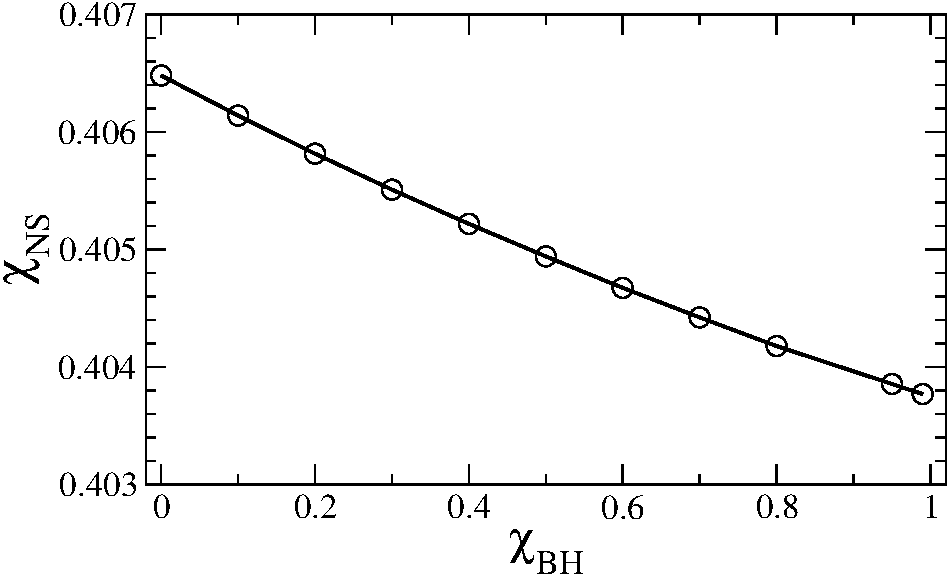
\includegraphics[scale=0.95]{chap4/chichi}}
\caption[Measured neutron star spin plotted as a function of black
  hole spin.]{\label{fig:chichi}Neutron star spin $\chi_{\rm NS}$ as a
  function of black hole spin $\chi_{\rm BH}$ for this sequence. We
  notice a small downward linear trend.}
\end{figure}
%%%%%%%%%%%%%%%%%%%%%%%%%%%%%%%%%%%%%%%%%%%%%%%%%%%%%%%%%%%%%%%%



Finally, we consider a sequence of initial-data sets that varies the
mass ratio from $q=2$ to $q=10$. In this sequence we keep the other
binary parameters the same as in the ${\tt R14i0\Uparrow}$ initial
data set and we keep the orbital parameters $M\Omega$ and $D/M$
constant.

As the mass-ratio changes, we expect that the orbital frequency needed
to achieve low eccentricity will also somewhat change. We do not
model this effect, but rather keep all other binary parameters are the
same as in the {\tt R14i0$\Uparrow$} run. In particular, the orbital
parameters $M\Omega$ and $D/M$ are constant. While not the most
accurate way of choosing these parameters, as it is only correct to
Newtonian order, it suffices for the present purpose of testing
robustness of the initial-data solver.

To estimate the impact on the eccentricity of the constructed
initial-data sets, we use the post-Newtonian expansion of the orbital
frequency of a BBH in a {\it circular} orbit (Eq. 228 of
\cite{Blanchet2006}):
\begin{equation}
\Omega^2=\frac{GM}{r^3}\left(1+(-3+\nu)\gamma+\left(6+\frac{41}{4}\nu+\nu^2\right)\gamma^2+...\right).
\end{equation}
Here $\nu=m_1m_2/(m_1+m_2^2)=q/(1+q)^2$ is the symmetric mass ratio, and
$\gamma=GM/Dc^2$. Keeping $D$ and $M$ constant, the quantity $M\Omega$
varies by approximately 3\% in the mass ratio range we consider.
Therefore, we expect that the eccentricity of our initial-data sets varies
by only a few percent between $q=2$ and $q=10$.


%%%%%%%%%%%%%%%%%%%%%%%%%%%%%%%%%%%%%%%%%%%%%%%%%%%%%%%%%%%%%%%%
\begin{figure}
\centerline{\hspace*{1.5cm}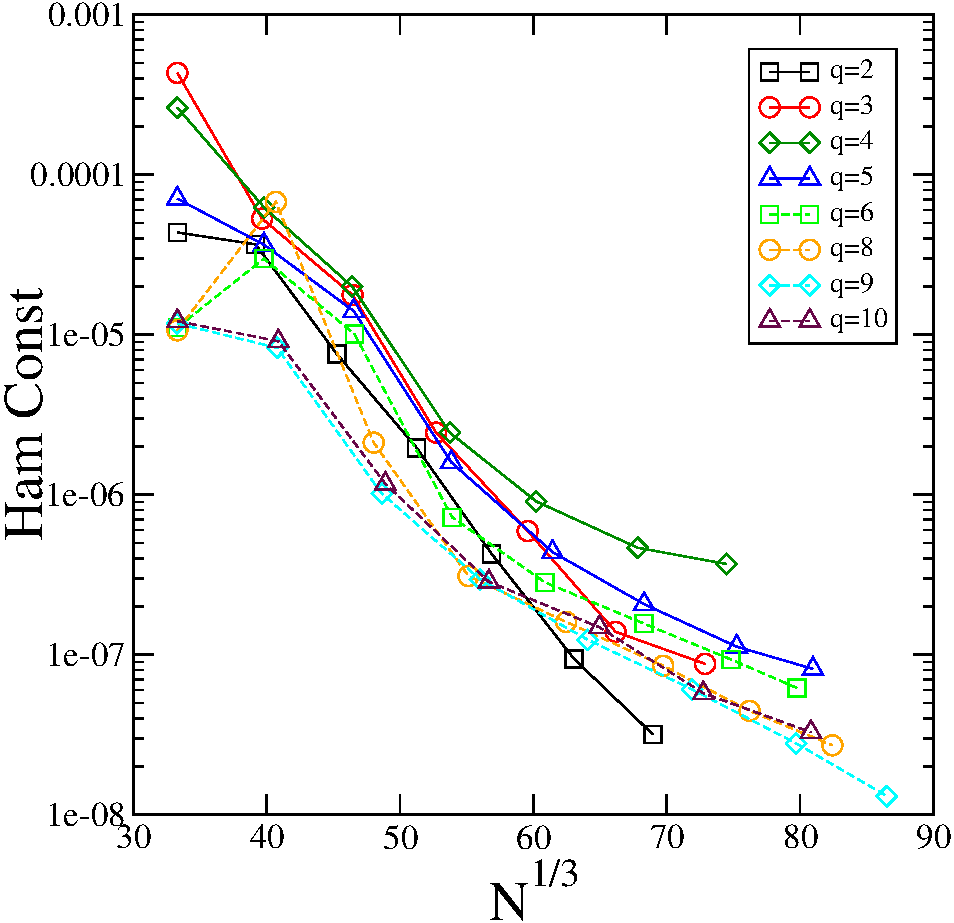
\includegraphics[scale=0.95]{chap4/qSeqHam}}
\caption[Hamiltonian and momentum constraint for the $q$
sequence.]{\label{fig:qSeqHam}Hamiltonian constraint (top panel) and
  momentum constraint (bottom panel) versus resolution for our
  sequence of binaries where the mass ratio is varied from $q=2$ up to
  $q=10$. The NS spin parameter is kept constant at
  $\vec\omega_{\rm NS}=0.017\hat z$ and the black hole spin is
  $\chi_{\rm BH}=0.9$. }
\end{figure}
%%%%%%%%%%%%%%%%%%%%%%%%%%%%%%%%%%%%%%%%%%%%%%%%%%%%%%%%%%%%%%%%

To assess convergence, we plot the Hamiltonian and momentum
constraints for this sequence in Fig.~\ref{fig:qSeqHam}. We find
exponential convergence in all cases. Interestingly, no clear pattern
in $q$-space emerges.

Figure~\ref{fig:qchi} plots the neutron star spin as a function of mass-ratio.
Having kept $\vec\omega_{\rm NS}$ constant across this sequence, 
we indeed find that the physical NS spin is approximately constant, too, varying less than $2$ percent.  Although there is not a great amount of variation,
apart from $q=2$, there is a clear trend of $\chi_{\rm NS}$ decreasing
with $q$. Again, however, the effect is quite small and we do not seek
to explain it.

%%%%%%%%%%%%%%%%%%%%%%%%%%%%%%%%%%%%%%%%%%%%%%%%%%%%%%%%%%%%%%%%
\begin{figure}
\centerline{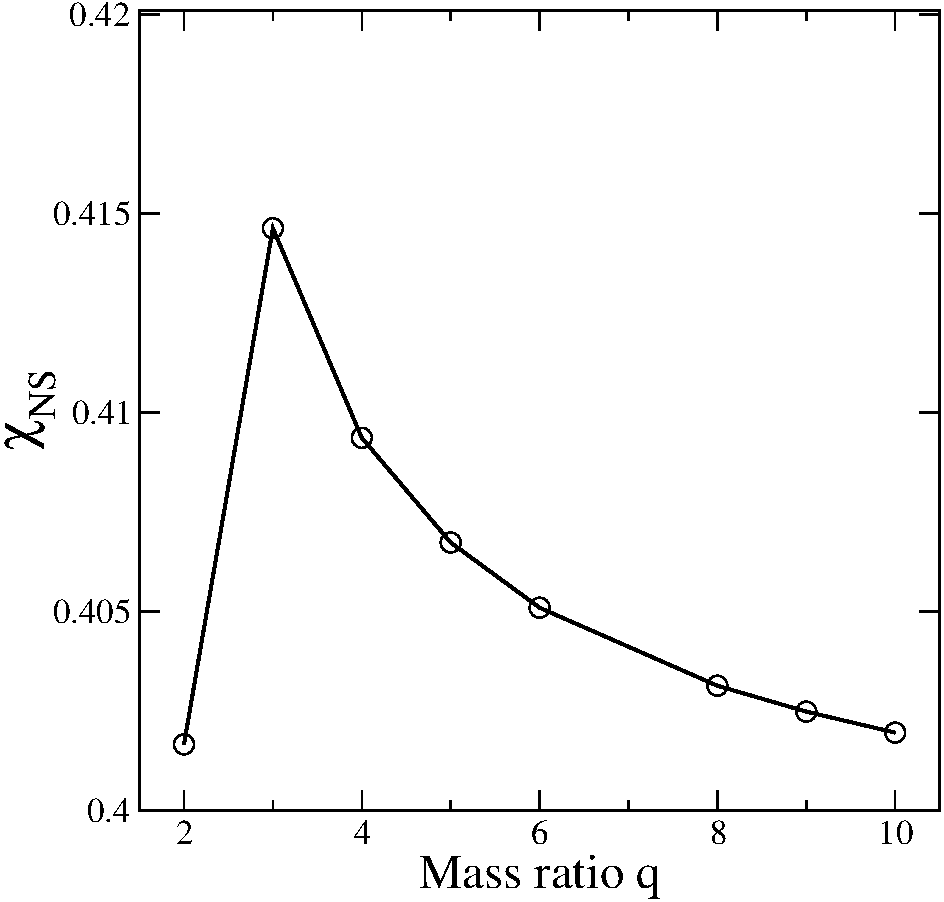
\includegraphics[scale=0.95]{chap4/qchi}}
\caption[$\chi_{\rm NS}$ as a function of mass ratio
$q$.]{\label{fig:qchi}Neutron star spin $\chi_{\rm
    NS}$ as a function of mass ratio $q$ for this sequence. We notice
  a small downward trend for $q \geq 3$.}
\end{figure}
%%%%%%%%%%%%%%%%%%%%%%%%%%%%%%%%%%%%%%%%%%%%%%%%%%%%%%%%%%%%%%%%


\section{Conclusion}
\label{sec:Conc}


In compact object binaries containing neutron stars, the spin of the
neutron star(s) forms part of the parameter space of such binaries.
In order to constrain neutron star spin {\it directly from
  gravitational wave observations}, one must know the impact of the
neutron star spin on the evolution of the compact object binary,
i.e. on the emitted waveforms and on the electro-magnetic signature.

This chapter lays foundations for such studies by constructing
initial-data sets of BH-NS binaries with arbitrary neutron star spins.
To our knowledge, this is the first time initial data has been created
for BH-NS binaries with spinning neutron stars. To impart spin on the
neutron star, we carry over the formalism developed
by~\cite{Tichy:2011gw} and used
in~\cite{Bernuzzi:2013rza,Tacik:2015tja,Dietrich:2015pxa} to create
initial data for NS-NS systems with arbitrary spins.

Two new numerical tricks were found to be necessary to get convergent
initial data - setting a maximum radius out to which to apply
$W^i=\epsilon^{ijk}\omega^jr^k$, and only activating the neutron
star spin after the first AMR-iteration of the initial data solver has
completed. We create initial data sets across a large
portion of the BH-NS binary parameter space. 

First, we present a comprehensive study of initial-data sets with various NS spins, restricting to $q=7$ and $\chi_{\rm BH}=0.9$.
This first study spans three different equations of state (all
$\Gamma=2$ polytropes), different neutron star spin magnitudes,
different neutron star spin orientations, and four different black
hole spin orientations. Subsequently, we construct initial data with
spinning NS for mass-ratios from $q=2$ to $q=10$, and for black-hole
spins $0\le \chi_{\rm BH}\le 0.99$, the latter well exceeding the
standard Bowen-York limit on black hole
spin~\citep{Lovelace2008,DainEtAl:2008}. Finally, we explore the range
of possible NS spin magnitudes, and find that the presented numerical
techniques can successfully construct initial data with neutron star
spins ranging from $\chi_{\rm NS}=0$ to $\chi_{\rm NS}\sim0.7$ (near
the maximum theoretical spin for neutron stars).

Future research will involve running evolutions of these, or similar,
initial data sets. Some of the 36 initial data sets of our first study
(Table~\ref{tab:36Sets}) can be used to investigate how neutron star
spin affects tidal disruption of the star by the black hole, and how
it affects the disk that is formed. The orbital phase evolution can
also be examined and compared to Post-Newtonian~\citep{Blanchet2014} or
other analytic predictions such as Effective-One-Body
(EOB)~\citep{Buonanno99,Taracchini:2013rva,Pan:2013rra}. 


One can also explore the maximum mass of accretion disks and ejecta as
a function of NS spin.~\cite{Lovelace:2013vma} finds a very large
disk with a black hole spin of $\chi=0.97$ and mass ratio $q=3$. Keeping these BH and NS parameters, but adding spin on the neutron star will cause the NS' material to be less strongly bound and may increase the disk mass even further.





\chapter{Junk Radiation in Binary Black Hole Simulations}

%\section{Chapter Overview}
%
%An Overview of my chapter here.
%
%

%\section{Chapter TDL}
%\begin{itemize}

%\item Many citations in the introduction and very much out of
 % date. It should be re-written.

%\item Are there any new papers on junk radiation to discuss that have
 % come out since this time? Ask Harald / do a literature search.

%\item Discuss more about boundary conditions in IVP for bbh

%\item Maybe make a table detailing all the simulations that were
 % done. Come up with a better naming system for the runs.

%\item There is a note about the uncertainity from numerical
 % trunctation in $E_J$ for SKS. Not sure what to do about that. I
  %think it can reasonably left the way it is.

%\item Combine data into a single plot for wave extraction plot

%\item Decide what to do for $\delta M$ for SKS, given that the data is
 % so weird

%\item Write the results section closely citing all the figures
 % properly. Are we overfitting the data? Be careful with how to report
  %the data. Maybe just focus on the plots, and not the fits.

%\item Write a conclusion. What are the implications of these kinds of
 % numbers?

%\end{itemize}


\section{Introduction}
The detection of the inspiral and merger of binary black holes by
Advanced
LIGO\big[\cite{PhysRevLett.116.241103},~\cite{Abbott:2016blz}\big] has
dawned the beginning of the era of gravitational wave astronomy. To
make these kind of detections, and to learn about the properties of
the source, gravitational waveform templates must be accurately
modelled. Although analytic perscriptions like Post-Newtonian (PN)
\big[\cite{Blanchet2006}\big] or Effective One-Body (EOB)
\big[\cite{Buonanno99}\big] can accurately model some of the inspiral,
Numerical Relativity (NR) simulations are needed to accurately model
the late inspiral and merger of the black holes.

In current NR simulations, there is always a burst of spurious
gravitational radiation at the start of the simulation, often referred to as
``junk radiation''. This pulse
always occurs at the start of the simulation, it is of much higher frequency and amplitude
than the astrophysical gravitational radiation, and it has significant
contributions from modes other than the standard $(l,m) = (2,2)$
spherical harmonic mode, which is the dominant contribution for the
astrophysical part of the waveform.  Therefore, this pulse is not astrophysical.

We illustrate this effect in Fig.~\ref{fig:Typical}, showing the
gravitational waveform  at the start of a
typical simulation. The waves are extracted on a coordinate sphere at
$r=160M$ \footnote{We use units where $G=c=1$. The only natural length
  and time scale is then the total mass of both black holes, $M$.}, so
the waves start appearing at $t\approx 160M$. We see the burst of junk
radiation last about $100M$ in time, with significant contributions
from both the $(2,2)$ and $(2,0)$ modes. The junk radiation then dies out,
and subsequently, the expected sinusoidal $(2,2)$ mode emerges.

\begin{figure}
 \includegraphics[scale=0.95]{chap5/Typical}
  \caption[A typical run illustrating junk radation.]{A typical run illustrating the spurious burst of junk radiation. We see at early times a burst of high-frequency, high-amplitude radiation. At later times, the $(2,0)$ mode dies out, and the $(2,2)$ mode settles into the usual inspiral-type radiation}
  \label{fig:Typical}
\end{figure}


This junk radiation is undesirable in simulations for several
reasons. It adds to the computational cost of the simulation as the
junk radiation must leave the computational grid before any useful
physical information can be extracted.  It can unrealistically shorten
the time until the black holes
merge \big[\cite{BodeEtAl:2008}\big]. It also makes it more difficult
to compare general relativistic simulations with Post-Newtonian
calculations. It is therefore a useful endeavour to try to better
understand the junk radiation, how important it is, and how to reduce
it.

Junk radiation is thought to be caused by assumptions made during the
initial data construction, which are not compatible with binary black holes in perfect equilibrium. Specifically,
 black holes are generally treated in the
initial data as independent and non-interacting, while in reality
there should be some non-trivial tidal interactions between them
(see~\big[\cite{Chu:2013nkx,JohnsonMcDaniel:2009dq}\big] for examples of including tidal interactions). If
we consider a sequence of initial data sets where the initial
separation between the holes is decreasing, we would expect that this
effect becomes more important as the initial separation
decreases. Similarly, there should be some outgoing gravitational
radiation already present in the simulation to model the black holes
inspiraling from infinity, and this is generally not modelled (see~\big[\cite{JohnsonMcDaniel:2009dq,Kelly:2009js}\big] for efforts to model it).
Moreover, the black holes in the initial data are often constructed
with techniques that do not even allow to construct a single, equilibrium black  hole.  Specifically, often, conformal flatness is assumed. As detailed in section~\ref{subsec:IVP}, the construction of initial data has a
free choice for the conformal metric, $\tilde{g}_{ij}$, on the initial
hypersurface. A common choice is conformal flatness, i.e.,
$\tilde{g}_{ij}$ is equal to the flat Euclidean metric. Since every
spherically symmetric space is conformally flat, this would be fine
for one Schwarzchild black hole. However,  a
binary system of compact objects is not conformally flat at second PN
order \big[\cite{Rieth:1997}\big], and the Kerr space-time does not admit a
conformally flat slicing that continuously approach Schwarzschild
coordinates as the spin goes to zero \big[\cite{GaratPrice:2000}\big]. 
The former effect should decrease in importance with increasing separation of the binary.  The latter is caused by a deficiency of conformally flat slicing that is present even for single spinning black holes, and so we expect its importance
to be approximately independent of binary separation.
% It is reasonable to think that the latter
% effect becomes more important for initial data where the black holes
% have higher spins, while we might imagine that the first effect is
% some sort of constant effect.

\cite{Lovelace2009} investigated the effects on junk radiation of using
superposed Kerr-Schild~\big[\cite{Matzner1999,Marronetti-Matzner:2000,Pfeiffer2002a,Lovelace2008}\big] (conformally curved) initial data for equal mass, non-spinning black
holes.  The conformal metric is written as
\begin{equation}
\tilde{g}_{ij}=f_{ij}+e^{-(r_A/w)^2}\left(g_{ij}^A-f_{ij}\right)+e^{-(r_B/w)^2}\left(g_{ij}^B-f_{ij}\right),
\end{equation}
where $f_{ij}$ is the Euclidean metric, $r^{A,B}$ are the distances
from black holes $A$ and $B$, and $g_{ij}^{A,B}$ is the Kerr-Schild metric boosted in
the direction of the black hole's motion. This has the effect that the
metric looks like Schwarzschild near the black holes, and looks flat
far away. The Gaussian scalings were needed to help improve the
convergence of the initial data. It was found that in general, the
conformally curved initial data can decrease the amplitude of the junk
radiation by a factor of $\sim 2$.
Superposed Kerr-Schild initial data is built around the
  Kerr-Schild metric, which exactly represents single spinning black holes.
 Therefore, one would expect that the advantages of superposed Kerr-Schild become particularly apparent for spinning black holes.

In this paper we investigate the parameter space dependence of junk
radiation. We measure its dependence on the spin and on the initial
separation of the black holes, for low eccentricity, equal-mass,
spin-aligned binaries. We also perform a comparison between conformally
flat (CF) initial data, and superposed Kerr-Schild (SKS) initial data. To
quantify the amount of junk radiation present we will use three
diagnostics - the amount of energy present in the junk radiation, and
the size of the transient effects of mass increase and spin decrease
due to the junk radiation.

This chapter is organized as follows: 
  Section~\ref{sec:NumericalMethods} presents the numerical methods,
  and Section~\ref{sec:Methodology} describes how we quantify junk
  radiation and other initial transients in the BBH initial data sets.
  We present our results in Sec.~\ref{sec:Results} and close with a discussion in Sec.~\ref{sec:JRDiscussion}.

\section{Numerical Methods}
\label{sec:NumericalMethods}

\subsection{The Initial Value Problem}
\label{subsec:IVP}
Employing the usual 3+1 decomposition(~\cite{ADM,york79}),space-time is foliated by a family
of spacelike hypersurfaces $\Sigma_t$. Each hypersurface has a
future-pointing unit normal $n^{\mu}$, induced metric $g_{ij}$, and
extrinsic curvature
$K_{\mu\nu}=-\frac{1}{2}\mathcal{L}_{n}g_{\mu\nu}$. The metric is
written as 
\begin{equation}
g_{\mu\nu}=-\alpha^2dt^2+g_{ij}\left(dx^i+\beta^idt\right)\left(dx^j+\beta^jdt\right),
\end{equation}
where $\alpha$ and $\beta$ are the lapse function and the shift vector
respectively. The lapse measures the proper time between neighbouring
hypersurfaces, and the shift vector determines how coordinate labels
move between neighbouring hypersurfaces.  On the initial
hypersurface $\Sigma_0$, spatial metric and extrinsic curvature must satisfy the vacuum
constraint equations
\begin{eqnarray}
R+K^2-K_{ij}K^{ij}&=&0, \\
\nabla_j\left(K^{ij}-g^{ij}K\right)&=&0.
\end{eqnarray}
% They are then evolved in time by the vacuum evolution equations
% \begin{eqnarray}
% \partial_tg_{ij}&=& blahblah \\
% \partial_tK_{ij}&=& blahblah 
% \end{eqnarray}
To solve the constraint equations \ one writes(~\cite{Lichnerowicz44})
the metric in terms of a conformal metric $\tilde{g}_{ij}$ and a
conformal factor $\Psi$:
\begin{equation}
g_{ij}=\Psi^4\tilde{g}_{ij}.
\end{equation}
We also split the extrinsic curvature into trace and trace-free parts
\begin{equation}
K^{ij}=A^{ij}+\frac{1}{3}g^{ij}K,
\end{equation}
and employ the extended conformal thin sandwich formalism~\cite{York1999,Pfeiffer2003b} to further
decompose $A^{ij}$.  One must then choose
$\left(\tilde{g}_{ij},\partial_{t}\tilde{g}_{ij},K,\partial_{t}K\right)$
as the free data.  Compared to the extrinsic curvature decomposition~\cite{Murchadha-York:1974b}, the conformal thin sandwich formalism allows for 
physically motivated choices to a larger number of the free data.  Elliptic equations
with appropriate boundary conditions are then solved for $\Psi$,
$\alpha\Psi$, and $\beta^i$, and the physical data is
re-assembled. $\partial_t\tilde{g}_{ij} = \partial_tK = 0$ is chosen
so that system is initially stationary in the co-rotating
frame.  This then leaves $\tilde{g}_{ij}$ and $K$ as the free data to
choose.  

The two types of initial data we compare are described in detail in
~\cite{Lovelace2008}: Conformally flat, quasi-equilibrium initial
data employs conformal flatness, $\tilde{g}_{ij}=f_{ij}$, maximal
slicing, $K=0$, and inner
boundary conditions that enforce that the black holes are
instantaneously in
equilibrium~\big[\cite{Caudill-etal:2006,Cook2004,Cook2002}\big].  Superposed
Kerr-Schild initial data, first used
in\big[~\cite{Marronetti-Matzner:2000,Matzner1999}\big], takes the spatial
metric and extrinsic curvature as superposition of elements of
Kerr-Schild metrics (one for each black hole).  As explained in
\cite{Lovelace2008}, we introduce Gaussian attenuation functions
to ensure regularity at spatial infinity. The details on the inner
boundary conditions used can be found in ~\cite{Lovelace2008}.



\subsection{Code}
\label{sec:Code}

The initial data is solved using the spectral solver {\tt Spells}~\big[\cite{Pfeiffer2003}\big] of the Spectral 
 Einstein Code {\tt SpEC}\footnote{\url{www.black-holes.org}}. This is a
multi-domain elliptic PDE solver that uses pseudo-spectral methods,
whereby quantities of interest are expressed as a linear summation of
basis functions. This method gives exponential convergence (with the
number of basis functions) as long as the quantities of interest are
smooth. The black hole singularities are dealt with by excision from
the computational grid. We use the dual frame method described in
\cite{Scheel2006}. The domain decomposition and position of the black
holes are fixed in a comoving frame, but the equations of motion are
solved in an inertial frame that is asymptotically Minkowski. The
frames are related by a rotation term (due to orbital motion) and a
contraction term (due to inspiral motion).

Gravitational waves are extracted on outer spherical shells of the
domain using the Newman-Penrose scalar $\Psi_4$. Given a spacelike
hypersurface with unit normal $n^{\mu}$ and a spatial unit vector in
the direction of wave propagation $r^{\mu}$, $\Psi_4$ is defined as 
\begin{equation}
\Psi_4 = -C_{\alpha\mu\beta\nu}l^{\mu}l^{\nu}m^{\alpha}\bar{m}^{\beta},
\end{equation}
where $C_{\alpha\mu\beta\nu}$ is the Weyl tensor,
$l^{\mu}=\left(n^{\mu}-r^{\mu}\right)/\sqrt{2}$ and $m^{\mu}$ is a
complex null vector satisfying $m^{\mu}\bar{m}_{\mu}=1$. We then expand
$\Psi_4$ in spin-weighted spherical harmonics
\begin{equation}
\Psi_4(t,r,\theta,\phi)=\sum_{l=2}^{l_{\rm max}}\sum_{|m|\leq~l}{\Psi_4^{lm}(t,r)_{-2}Y_{lm}(\theta,\phi)}
\end{equation}
The number of terms used in this expansion is generally $l_{\rm max}\leq 8$ in
our simulations. At large $r$, $\Psi_4$ is related to the
gravitational wave amplitude, $h$, by
\begin{equation}
\Psi_4=\frac{d^2}{dt^2}h_{+}-i\frac{d^2}{dt^2}h_{\times}.
\end{equation}


\subsection{Eccentricity Reduction}
Gravitational radiation tends to circularize in-spiralling compact
binaries~\big[\cite{PetersMathews1963,Peters1964}\big]. We reduce orbital
eccentricity with an iterative method similar to the one described in~\big[\cite{Boyle2007,Chu2009}\big]. One selects the initial orbital
frequency $\Omega_0$ from Kepler's third law or from a Post-Newtonian
calculation, while assuming that the initial radial velocity, $v_r$ is
zero. After the first simulation has run for a sufficient length, about two orbits, we fit the time derivative of
the orbital frequency, $\dot{\Omega}(t)$ as suggested
in~\cite{Buonanno:2010yk}.  We fit parameters $\{A_0, A_1, t_c, B, \phi, \omega, q\}$ with the function
\begin{equation}
\dot{\Omega}(t)=A_0\left(t_c-t\right)^{-11/8}+A_1\left(t_c-t\right)^{-13/8}
+B\cos\left(\varphi + \omega
  t+qt^2\right),
\end{equation}
where $t_C$ is the time of merger. The first two terms represent the
smooth inspiral motion of the black holes, while the oscillatory
second terms represents unwanted effects due to eccentricity. The
updating formulae
\begin{equation}
\delta\Omega_0=-\frac{B\omega\sin{\varphi}}{4\Omega_0^2}
\end{equation}
\begin{equation}
\delta v_r = \frac{B d_0\cos{\varphi}}{2\Omega_0},
\end{equation}
where $d_0$ is the binary separation, are designed to circularize low eccentricity Newtonian binaries. This
process is continued iteratively, typically another one or two times,
until the eccentricity is reduced to $e\lesssim 0.002$. The effect of
eccentricity on junk radiation is discussed in section~\ref{subsec:ErrorEstimation}.

%
%\begin{eqnarray}
%\dot{\Omega}(t)&=&A_0\left(T_c-t\right)^{-11/8}+\\
%&&A_1\left(T_c-t\right)^{-13/8}+B\cos\left(\omega
 % t+\varphi+qt^2\right)
%\end{eqnarray}

%Gravitational radiation tends to circularize in-spiralling compact objects~\cite{PetersMathews1963,Peters1964}.  We reduce orbital eccentricity with an 
%iterative method similar
%to the one described in Refs.\cite{Boyle2007,Chu2009}.  One 
%guesses the initial orbital frequency $\Omega_0$ from Kepler's law or
%a Post-Newtonian calculation, while assuming that the initial radial
%velocity is zero. The time derivative of the black holes is then fit
%with five parameters
%\begin{equation}
%\dot{d}(t)=A_0+A_1t+B\sin(\omega t+\varphi)
%\end{equation}
%The first two terms represent the smooth inspiral motion of the holes,%
%while the \{oscillatory} second term represents unwanted effects due to
%eccentricity. In a Newtonian orbit, the eccentricity would be
%\begin{equation}
%e=\frac{B}{\omega d_0}.
%\end{equation}
%The values of $\Omega_0$ and $v_r$ are adjusted to make $B$ as small
%as possible, using
%\begin{equation}
%\delta\Omega_0=-\frac{B\omega\cos{\varphi}}{2d_0\Omega_0},
%\end{equation}
%\begin{equation}
%\delta v_r = -\frac{B\sin{\varphi}}{2}.
%\end{equation}
%These formulae are designed such that they circularize
%low-eccentricity Newtonian orbits. This process is continued
%iteratively, typically once or twice, until the
%eccentricity reduced to  $e\lesssim 0.002$.

%\red{[Only describe what you do: Combine the preceding and following
 % paragraphs, only leaving the equations you do actually use.]}
%In our simulations we used a similar procedure, but instead we fit
%the time-derivative of the orbital frequency, $\dot{\Omega}$, as suggested
%in~\cite{Buonanno:2010yk}. The fit is
%\begin{eqnarray}
%\dot{\Omega}(t)&=&A_0\left(T_c-t\right)^{-11/8}+\\
%&&A_1\left(T_c-t\right)^{-13/8}+B\cos\left(\omega
 % t+\varphi+qt^2\right)
%\end{eqnarray}
%and the updating formulae are:

%\begin{equation}
%\delta\Omega_0 = -\frac{B\omega\sin{\varphi}}{4\Omega_0^2}
%\end{equation}red
%\begin{equation}
%\delta v_r = \frac{B d_0}{2\Omega_0}\cos{\varphi}
%\end{equation}

%The effect of orbital eccentricity on junk radiation is discussed in
%section ~\ref{subsec:EccentricityEffect}

\subsection{Simulations}

We run BBH evolutions using both conformally flat and SKS initial
data.  We consider five different initial separations for CF data,
$D/M=\{12,15,20,25,30\}$, and $D/M=\{12,15,20\}$ for SKS data, where $M$ is the total mass of both black
holes, and at each separation we consider  six different spins,
$\chi=\{0,0.1,0.2,0.3,0.4,0.5\}$. In each case the black holes are of
equal mass, equal spin, and the spin is aligned with the orbital
angular momentum, i.e., in the the $+\hat{z}$ direction. To test the
convergence of our measurements, each run is done at four
resolutions, which we will refer to as {\tt N0} (lowest resolution) to
{\tt N3}
(highest resolution). Each evolution is
run to about $t\sim1000M$, which is long enough to accurately measure the
eccentricity, and make sure that it is sufficiently low. As discussed in
section~\ref{subsec:ErrorEstimation}, sufficiently low means
$e\lesssim 0.002$.

%%%%%%%%%%%%%%%%%%%%%%%%%%%%%%%%%%%%%%%%%%%%%%%%%%%%%%%%%%%%%%%%
\section{Methodology}
\label{sec:Methodology}
%%%%%%%%%%%%%%%%%%%%%%%%%%%%%%%%%%%%%%%%%%%%%%%%%%%%%%%%%%%%%%%%

We employ three diagnostics to measure the initial relaxation of
the initial data: the outgoing pulse of radiation (junk radiation),
the change in black hole mass during relaxation, and the change in
black hole spin during relaxation.



\subsection{Pulse in the Gravitational Waveform}

In this section we discuss our methods of
quantifying the amount of junk radiation present in a given
simulation. It is not immediately obvious what the best way to do this
is.  \cite{Lovelace2009} considered the
maximum value of the Newman-Penrose waveform,
$\max\{R|\Psi_4^{lm}|\}$, where $R$ is the extraction radius of the gravitational waves.  The
  $(l,m)=(2,2)$ and $(2,0)$ modes were found to dominate. We find,
  however, that this method has some inadequacies. This is illustrated
  by comparing $R|\Psi_4^{lm}|(t_R)$, where $t_R$ is the retarded time,
  $t_R=t-R$, in two different simulations. These use CF data, with the parameters $\{D=15M$, $\chi=0.2\}$; one is at our
  typical highest resolution {\tt N3}, and another at an even higher
  resolution, {\tt N7}. In terms of the total number of basis
    functions $X$, $X^{1/3}\sim58$ for {\tt N3} and $X^{1/3}\sim78$ for
    {\tt N7}. The $(2,0)$ and $(2,2)$ modes are shown in the top panel of
  Fig.~\ref{fig:HighResComparison}. It is clear that the $(2,0)$ mode
  is significantly different between {\tt  N3} and {\tt N7}, in both the
  largest peak and in the subsequent smaller peaks, and that these
  differences are not well encapsulated simply by using
  $\max\{R|\Psi_4|\}$. In Fig.~\ref{fig:HighResComparison} we also
  show these quantties for an SKS run with the same parameters. Because
  the waveform is significantly different from the CF waveform in both the
  number of peaks and their relative heights, it is clear that
  $\max\{R|\Psi_4^{lm}|\}$ does not encapsulate this waveform very well.

%\red{[Shorten this paragraph, combine with above.  The purpose of this paragraph is to explain why we do not follow Lovelace 2009, and this can be done with fewer words.  Although it would be handy to have a SKS Psi4 waveform, to further illustrate the problems. 
%]}
%We find, however, that this method presents several problems.  We compare two runs with evolution parameters $D=15M$ and
%$\chi=0.2$ and conformally flat initial data. One run
%is at our normal highest resolution, Lev3, and another is a very high
%resolution at Lev7. In terms of total number of basis functions, N, these
%resolutions are $N^{1/3}=57.93$ and $N^{1/3}=78.04$, respectively. In
%Fig.~\ref{fig:HighResComparison} we show the junk radiation
%content of the $(2,0)$ and $(2,2)$ modes for both of these runs.\note{Somewhere in here discuss the SKS part of fig2} The
%$(3,2)$ mode also has a significant contribution, but it is omitted
%for clarity. Clearly $\max\{r|\Psi_4^{lm}|\}$ has a quite
%strong dependence on resolution, especially in the $(2,0)$ mode. However,
%another problem is quite evident. For the $(2,0)$ mode, the first peak
%is much higher at Lev7, but the second peak is close, and all
%subsequent peaks are significantly smaller. Thus, in using
%$\textnormal{max}\{r|\Psi_4^{l,m}|\}$, important features in the junk
 %radiation are lost. Thus we conclude
%that $\textnormal{max}\{r|\Psi_4^{l,m}|\}$ is not a suitable diagnostic 
%for the amount of junk radiation.

\begin{figure}
  \includegraphics[scale=0.95]{chap5/HighResComparison}
  \caption[Junk radiation profiles for CF and SKS initial data, and a
  comparison to high resolution SKS initial data.]{{\it Top Panel:} Comparison of the junk radiation profiles for our usual
    highest resolution ({\tt N3}) and an additional run at very highest
    resolution ({\tt N7}). We see, especially for the $(2,0)$ mode, that the
    maximum peak of the junk radiation is much higher for {\tt  N7}, but
    additional peaks are comparable or higher for {\tt N3}. \newline {\it
      Bottom Panel:} Junk radiation profile for an SKS run with the
    same parameters as in the top panel. The waveform is significantly
    different in structure from the CF waveform.
}
  \label{fig:HighResComparison}
\end{figure}

As a more robust quantity that incorporates the whole waveform, and is
less resolution dependent than $\max\{R|\Psi_4^{lm}|\}$, we look at the
total energy carried away from the system by gravitational waves. The
 gravitational wave energy flux is~\big[\cite{Boyle:2008}\big]
\begin{equation}
F(t) =\frac{1}{16\pi}\sum_{l,m}\dot{h}_{lm}^2(t),
\end{equation}
where
\begin{equation}
\dot{h}_{lm}(t)=\int_{t_0}^{t}{\Psi_4^{lm}(t')dt'} + H_{lm}.
\end{equation}
The $H_{lm}$ are integration constants.  To measure the
  initial pulse of radiation, we use $t_0=0$ and $H_{lm}=0$.  The energy flux, $F(t)$, is shown in
the red curves in Fig.~\ref{fig:FluxSample} for conformally flat initial data (top
panel) and SKS initial data (bottom panel).  The initial burst
  is apparent in these figures; at late times $t_R\gtrsim 40M$, $F(t)$
  approaches the nearly constant energy flux of the astrophysical
  inspiral.  We are now faced with two problems: We would like to
  isolate the energy carried in junk-radiation from the energy-flux
  astrophysical inspiral.  And, we would like to do so in a robust way, 
independent of arbitrary choices.  We
  proceed as follows:

  First, we assume that the astrophysical energy flux begins at a time
  $t_{22}$, i.e.
\begin{equation}
  F_{22}(t) = F_0\,\theta(t-t_{22}).
\end{equation}
Here, $F_0$ represents the value of $F(t)$ after the pulse of
junk-radiation and $\theta$ represents the step-function.
The choice of a constant value $F_0$ is reasonable since the
timescale on which $F_{22}$ changes significantly is much longer than
the junk radiation timescale.
We will
discuss our choice for $t_{22}$ shortly.  The energy in the
junk-radiation is given by
\begin{equation}\label{eq:EJ}
E_J=\int_0^{t_C}\big[(F(t)-F_{22}(t)\big]dt,
\end{equation}
where the cut-off time $t_C$ is chosen after the junk radiation has
decayed, i.e. $t_C-R\gtrsim 50M$.  In Fig.~\ref{fig:FluxSample} we
plot a representative example of the computation of $E_J$ for CF (top
panel) and SKS (bottom panel) data. The blue dashed curves represent
$F_{22}(t)$, while the shaded area represents $E_J$.
%The energy attributed to the junk
%radiation is thus the shaded area in Fig.~\ref{fig:FluxSample}.  
As
already apparent from Fig.~\ref{fig:FluxSample}, the precise value of
$t_C$ is not extremely important, because at late times $F(t)-F_{22}(t)\approx 0$.  

It remains to chose a prescription for the choice of $t_{22}$, the
time when we deem the astrophysical waveform to ``turn on''.
% In finding the total energy in junk radiation, however, it cannot
% be assumed that all the energy emitted up to $t=t_C$ is due to junk
% radiation. The astrophysical $2,2$ mode signal, $F_{22}(t)$, should
% still be present, with the junk radiation signal superimposed on
% it. The energy in junk radiation is thus written as
% \begin{equation}
% E_J=\int_0^{t_C}\left(F(t)-F_{22}(t)dt\right)
% \end{equation}
% This quantity is represented by the shaded area in
% figure~\ref{fig:FluxSample}. We choose a simple model for $F_{22}(t)$:
% $F_{22}$ turns on at some time $t_{22}$ and takes on the constant
% value of $F_0=F(t_C)$. That is,
% \begin{equation}
% F_{22}(t)=F_0\theta\left(t-t_{22}\right)
% \end{equation}
% This is represented by the blue curves in
% figure~\ref{fig:FluxSample}. 
%The choice of a constant value for the flux is reasonable since the
%timescale on which $F_{22}$ changes significantly is much longer than
%the junk radiation timescale. 
%There is no a priori way to precisely
%determine where $t_{22}$ should be. 
A simple method would be to choose
$t_{22}$ to correspond to $\max\{F(t)\}$. This seems reasonable for
the conformally flat curve in Fig.~\ref{fig:FluxSample}, but the
more wide double-peaked structure of the SKS curve shows that another
approach is needed. Instead we take $t_{22}$ to correspond to the flux
weighted centre of the junk radiation waveform. The first moment of
$F(t)-F_{22}(t)$, in other words. So,
\begin{equation}\label{eq:t22}
t_{22}=\frac{\int_0^{t_C}{t\left(F\left(t\right)-F_0\theta\left(t-t_{22}\right)\right)dt}}{\int_0^{t_C}{\left(F\left(t\right)-F_0\theta\left(t-t_{22}\right)\right)dt}}.
\end{equation}
This equation must be solved iteratively for $t_{22}$, and the
solution is found to converge rapdily.

\begin{figure}
 \includegraphics[scale=0.95]{chap5/FluxSample}
  \caption[The flux, $F(t)$, and the computation of $E_J$ for CF and
  SKS intitial data.]{The flux $F(t)$ is plotted for two different runs, both
    with parameters $D=15M$ and $\chi=0$. Conformally flat initial
    data is in the top panel and SKS initial data is in the bottom
    panel. The solid red curve represents the total flux, $F(t)$. The
    dashed blue curve represents $F_{22}(t)$, the astrophysical flux
    that we subtract from $F(t)$. The shaded area between the two
    curves is the energy in junk radiation, $E_J$.
}
  \label{fig:FluxSample}
\end{figure}

\subsection{Uncertainty in $E_J$}
\label{subsec:ErrorEstimation}

%\subsubsection{Resolution of the Waveform}

Several effects may influence the quantity $E_J$ computed by
  Eqs.~(\ref{eq:EJ}) and~(\ref{eq:t22}).  {\it Numerical truncation
    error} can be estimated by performing the simulations with
  different numerical resolution.  Our simulations show that in general,
  $E_J$ increases with resolution. This is because junk radiation is
a short wavelength feature, so greater resolution allows for more of
the features present to be captured.  To estimate the
uncertainty in $E_J$, we compare our $\{D=15M$,
$\chi=0.2\}$ runs at {\tt N3} and {\tt N7}, as discussed earlier. We find that
at {\tt N7}, $E_J$ is about $13\%$ greater than at {\tt N3}. Since we don't
have such high resolutions runs available for each of our cases, we
assume that we can use this same $13\%$ difference for each of our
runs. We are also assuming that at {\tt N7} the junk
radiation is nearly fully resolved, so that this difference is a good
indication of the true value. Finally, we use this same uncertainty of
$13\%$ for the SKS runs as well - while the technology is different
for the SKS runs, it should still be a reasonably good estimate, and
likely a conservative estimate, of the numerical truncation error in them.

%\subsubsection{Choice of $t_C$}

A second uncertainty arises through the {\it choice of $t_C$}.
This number is chosen manually for
each run, introducing a
  subjective element into the analysis. Examining the flux curves in
Fig.~\ref{fig:FluxSample}, for example, $t_C$ could conceivably be
chosen differently by $\sim 10 M$ and still be a
reasonable choice. {Our definition Eq.~(\ref{eq:EJ}) was meant
to be robust to small changes in $t_C$.  For $E_J$ to be a robust measurement, it should
therefore not change significantly in response to changes $\delta t_C$
that are of that order. Indeed, this is enforced by our definition of
$E_J$, which subtracts out the additional flux in the astrophysical
$(2,2)$ mode.}  To verify this assertion, we compute $E_J$ with $t_C$ in Eq.~(\ref{eq:EJ}) replaced by $t_C+\delta t_C$.  Figure~\ref{fig:EvsDtC} shows that indeed $E_J$ is almost independent of $\delta t_C$.  
%The uncertainty introduced by $t_C$ is about $1\%$. 
In Fig.~\ref{fig:EvsDtC}, $E_J$ is plotted against $t_C$
in the representative $\{D=15M, \chi=0\}$ case.
For each run we define a fractional
error parameter due to the choice of $t_C$, where we average the
differences for $\delta t_C = -10M$ and $\delta t_C = 10M$:
\begin{equation}
\frac{\Delta E}{E} = \frac{|E_J(t_C+10M) - E_J(t_C)| + |E_J(t_C) - E_J(t_C -
  10M)|}{2E_J(t_C)}
\end{equation}
This uncertainty ranges from $\sim 0.25\%$ to $\sim 3.75\%$ throughout
all of our simulations.

\begin{figure}
 \includegraphics[width=0.95\columnwidth]{chap5/EvsDtj}
  \caption[$E_J$ as a function of $\delta t_C$.]{$E_J$ is plotted against $\delta t_C$, representing changes
    to the selected value of $t_C$ for runs where $D=15M$,
    $\chi=0$. The results for conformally flat initial data are shown
    in the top panel, and SKS initial data in the bottom
    panel. Typical changes in $E_J$ are on the order of a few
    percent.}
 \label{fig:EvsDtC}
\end{figure}


A third error in $E_J$ arises through {\it the finite radius
    of gravitational wave extraction}.  In this study, gravitational waves are extracted at radii $R_{\rm ex}\sim 300-400M$.  Gravitational waves extracted at finite radii are subject to near-field effects which may cause the extracted
waveforms to differ from the one that would be observed at
infinity.  
To estimate the error in $E_J$ due to the finite extraction radius, we
use the following procedure. For each of our simulations, we compute $E_J$ at
several extraction radii, and examine $E_J$ as a function of
$1/R_{ex}$. We then extrapolate
\begin{equation}
E_{\infty} = \lim_{1/R_{ex}\rightarrow 0}E_J(1/R_{\rm ex})
\end{equation}
using a linear fit in $1/R_{\rm ex}$ to estimate the behaviour of $E_J$ at infinity. We
then take the fractional difference
\begin{equation}
\frac{\Delta E}{E} = \frac{E_{\infty}-E_J}{E_J}
\end{equation}
as our error estimate. This parameter is on the order of $10\%$ for
most of our runs. Note, however, that we still use $E_J$ and not $E_{\infty}$ as
our measure of energy in the pulse. In Fig.~\ref{fig:EvsRextr} we illustrate an
example of this procedure, plotting $E_J$ vs. $1/R_{ex}$ for one case,
$\{D=15M, \chi=0\}$, for both CF and SKS data.

\begin{figure}
  \includegraphics[scale=0.95]{chap5/EvsRextr}
  \caption[$E_J$ as a function of $1_R/{\rm ex}$.]{$E_J$ as a function of $1/R_{ex}$, where $R_{ex}$ is the
    extraction radius. This is for the case where $\{D=15M,\chi=0\}$,
    with CF data in black and SKS data in red. The dashed lines
    represent the best linear fit. The extrapolation
    to $1/R_{ex}\rightarrow 0$ allows us to estimate the error on
    $E_J$ due to finite extraction radius effects. }

  \label{fig:EvsRextr}
\end{figure}

A final factor that could influence the estimated $E_J$ is the
{\it eccentricity of the orbit of the black holes}. Previously we argued
that it is important for astrophysically realistic binaries to have
low eccentricity. We now consider how it affects the junk radiation, specifically the effect on $E_J$. We examine the case $D=25M \chi=0.1$
for CF data, as this particular case led to a fairly large range of
eccentricities in the reduction process;
$e\sim\{0.03,0.008,0.0006\}$. The measured $E_J$ for these three cases
is $10^6E_J=\{7.053\pm0.38\%, 7.204\pm0.53\%, 7.174\pm0.58\%\}$. Here,
the quoted uncertainty is purely due to the choice of $t_C$. The
differences between the first two eccentricities is $2.10\%$ and it is
$0.42\%$ for the last two. Because the latter difference is less than
the uncertainty due to the choice of $t_C$, the two runs are
effectively indistinguishable, and we conclude that we can safely
ignore the effects of residual eccentricity once we have $e\lesssim
0.008$. However, to be ``safe'', we have generally reduced the
eccentricity of all of our runs to $e\lesssim 0.002$.

%\harald{A final factor influencing the estimated $E_J$ is the
%{\em eccentricity of the orbit of the black holes}. }
%\subsubsection{Effect of Eccentricity}
%\label{subsec:EccentricityEffect}
%\red{[As discussed: Remove Fig.~\ref{fig:EccComparison}, state here in main-text $E_J$ for the different eccentricities, conclude that the effect of eccentricity is below xxx.  Also shorten text, by removing unneeded words and information] }
%Previously, we argued that it is important for astrophysically
%realistic binaries to have low eccentricity. We now examine how
%eccentricity actually affects the junk radiation. In
%figure~\ref{fig:EccComparison}, we have plotted the leading order (2,0) mode
%of the junk radiation for eccentricities of $e\approx
%\{0.03,0.008,0.0006\}$. This was done for runs where $D=25M$,
%$\chi=0.1$, and at medium resolution, i.e. Lev2. This was chosen as it
%happened to give us the largest range of eccentricities available, and
%often the highest resolution Lev3 runs at higher eccentricity were
%terminated earlier. We find that the junk radiation amplitude is
%nearly independent of the eccentricity. Figure ~\ref{fig:EccComparison} shows
%that there is some visible difference between
  %$e\approx 0.03$ and $e\approx 0.008$, but nearly no difference
  %between $e\approx 0.008$ and $e\approx 0.0006$.  The impact of eccentricity
%on the junk-radiation is even smaller for the $(2,2)$
  %mode. Figure~\ref{fig:EccComparison} essentially shows that we can
  %safely ignore the effects of residual eccentricity once we have $e
  %\lesssim 0.008$. However, to be ``safe'', we have generally reduced
  %the eccentricity of all of our runs to $e\lesssim 0.002$.
%\begin{figure}
%\includegraphics[scale=0.5]{EccComparison}
 % \caption{\note{Kill this plot, and add words describing it to the text}\note{Define what is plotted.  If this is the integral of
%      $\dot h_{20}^2$, then wouldn't it be more suitable to plot
 %     $E(t)$ directly at different resolutions?  Include legend} A
   % comparison of the $2,0$ mode of junk radiation at three different
   % eccentricities. At the two lowest eccentricities, the junk
   % radiation profiles are essentially the same, telling us that we
   % can effectively ignore eccentricities under $e \sim
   % 0.008$}
 % \label{fig:EccComparison}
%\end{figure}

\subsection{Transient behaviour in Black Hole quantities}

\subsubsection{Mass Increase}
In addition to the energy carried away in junk radiation, we utilize two further
diagnostics of transients arising from imperfect initial data.
The first diagnostic comes from the irreducible
mass of the black hole, $M_{\rm irr} = \sqrt{A/16\pi}$, where $A$
is the area of the black hole's apparent horizon. In the first few $M$ during the evolution, the apparent horizon mass
$M_{\rm irr}(t)$ increases by a small amount, before settling down to
an approximately constant value. This effect is easily apparent for CF initial data plotted in the upper panel of Fig.~\ref{fig:MassIncreaseCFSKS}.
We characterize the increase in mass due to initial transients by 
\begin{equation}
\delta M(t)=\frac{M_{\rm irr}(t)}{M_{\rm irr}(0)}-1
\end{equation}
and we define the equilibrium parameter $\delta M = \delta M(t_{\rm eq})$.
Here $t_{\rm eq}$ is a time where the mass-increase is complete and
levels off; typically $\sim20M$. 

For SKS initial data the behaviour of $M_{\rm irr}(t)$ is more
  complex.  Within the first few $M$, $M_{\rm irr}(t)$ shows a rapid
  increase, presumably due to relaxation of the geometry
  in the immediate vicinity of the black holes.  The trend here is
  similar to the CF initial data, in that larger spins result in a
  larger increase of $M_{\rm irr}(t)$, albeit the magnitude of the
  increase is about a factor of 50 smaller for SKS initial data.
  Subsequently, starting at $t\sim 40M$, the SKS simulations show a second
  set of features, oscillations with amplitude $\sim 2\times 10^{-5}$ lasting about
  $60M$.  The features of these oscillations are similar to each other
  even for runs with different spin black hole spin $\chi$.  Therefore, it is
  likely that these oscillations are caused by features in the initial
  data set {\it away} from the black holes.

\begin{figure}[!htb]
 \includegraphics[width=0.95\columnwidth]{chap5/MassIncreaseCFSKS}
  \caption[Normalized irreducible mass curves for CF and SKS data.]{Normalized irreducible mass curves for CF data (top panel)
    and SKS data (bottom panel) for all of the different spins in the
    covered parameter space and $D=15M$ remaining constant. }
  \label{fig:MassIncreaseCFSKS}
\end{figure}

There is a clear qualitative difference between the CF and SKS
curves. The CF data evidently forms an increasing sequence of
$\delta_M$ with $\chi$, and $\delta_M$ is clearly well-defined in each
case. However, the SKS data exhibits oscillatory behavior that is
relatively spin-independent, and there is not a clear way to robustly
define $\delta_M$. To further underscore the difficulties of the SKS
data, figures~\ref{fig:CFMConvergence1} and~\ref{fig:SKSMConvergence1}
show convergence tests for one of the mass curves shown in
fig.~\ref{fig:MassIncreaseCFSKS}, $\{D=15M,\chi=0.3\}$. The top panels
of Figs.~\ref{fig:CFMConvergence1} and~\ref{fig:SKSMConvergence1} show
$M_{\rm irr}(t)$ of one of the black holes computed at different
numerical resolutions, and the bottom panels show differences in
$M_{\rm irr}(t)$ computed at neighboring resolutions. Note that our
parameter space studies presented in Sec.~\ref{sec:Results} were
usually performed on resolution {\tt N3}; we have run {\tt N4-N6} for
select cases to test convergence. The CF initial data shows rapid
convergence and the features in the upper panel of
Fig.~\ref{fig:CFMConvergence1} are well resolved. For the SKS data
shown in Fig.~\ref{fig:SKSMConvergence1} we do not find convergence -
the differences between resolutions do not strictly decrease with
increasing resolution, and these differences are of similar order to
the features that we are trying to quantify. Our conclusion is
therefore that the magnitude of the change $M_{\rm irr}(t)$ is much
smaller for SKS initial data than for CF initial data ($\sim 10^{-5}$
vs. $\sim 5\times10^{-4}$), however, the changes in $M_{\rm irr}(t)$
for SKS initial data approach our numerical truncation error, and are
furthermore ambiguous due to the extra oscillatory features present in
Fig.~\ref{fig:MassIncreaseCFSKS}. We therefore shall not attempt to
quantify them in detail, beyond giver upper bounds on $\delta_M$ for
the SKS data.

\begin{figure}
 \includegraphics[scale=0.95]{chap5/CFMConvergence1}
  \caption[Convergence of $M_{\rm irr})(t)$ for CF initial
  data.]{Convergence test of $M_{\rm irr}(t)$ for CF initial data in the
  case $\{D15=M,\chi=0.3\}$. The top panel shows $M_{\rm irr}(t)$ at
  different resolutions, and the bottom panel shows the difference
  between consecutive resolutions.}
  \label{fig:CFMConvergence1}
\end{figure}

\begin{figure}[!htbp]
 \includegraphics[scale=0.95]{chap5/SKSMConvergence1}
  \caption[Convergence of $M_{\rm irr})(t)$ for SKS initial
  data.]{Convergence test of $M_{irr}(t)$ for SKS initial data in the
  case $D15=M$, $\chi=0.3$. The top panel shows $M_{irr}(t)$ at
  different resolutions, and the bottom panel shows the difference
  between consecutive resolutions.}

  \label{fig:SKSMConvergence1}
\end{figure}

\subsubsection{Spin Decrease}

Our third and final quantification of junk radiation comes from the
black hole's spin $S(t)$. At early times in each simulation 
%--seen in Fig.~\ref{fig:SvsT2}
, the spin
of each black hole decreases and oscillates rapidly. Eventually, at
some time $t_{\rm eq}$, the spin reaches some approximately constant
value, which is lower than the initial spin, $S(0)$. This effect can
be interpreted as angular momentum being carried away from the system
by junk radiation. Note that we use the dimension-ful quasi-local
angular momentum, measured with approximate Killing vectors as
described in~\cite{Lovelace2008}. We use $S$ rather than $\chi=S/M^2$
to de-couple the change in spin from the change in mass. This effect
is illustrated in Fig.~\ref{fig:SvsT2}, where we plot $\delta~S(t)$
for all of our simulations done at $D=15M$.

Analogous to $\delta M(t)$, we can define the parameter $\delta S(t)$ as the
fractional spin decrease of the black hole:
\begin{equation}
\delta S(t)=\frac{S(t)}{S(0)} - 1
\end{equation}
and the equilibrium parameter $\delta S_{eq}=\delta S(t_{eq})$, where $t_{eq}$ the
time when $\delta S(t)$ has reached some nearly constant value.
In practice, we compute $\delta S_{eq}$ as the average value of
$\delta S(t)$
over some suitable interval around $t_{eq}$.

We find similar difficulties in defining $\delta~S$ for the SKS data
as we did for defining $\delta~M$. In Fig~\ref{fig:SvsT2}, the SKS
data shows similar oscillatory behavior that makes it difficult to
robsutly define $\delta S$. After the oscillations, $\delta S$ does
not neatly form a monotonic sequence in $\chi$.
Analogous to Figs.~\ref{fig:CFMConvergence1}
and~\ref{fig:SKSMConvergence1}, Figs.~\ref{fig:CFSConvergence1} and
~\ref{fig:SKSSConvergence1} demonstrate convergence tests for $\delta
S(t)$, again for the case $\{D=15M,\chi=0.3\}$. Similar to what was seen
in the convergence test for $M_{\rm irr}(t)$, the CF data convergences
rapidly, while we see no clear convergence in the SKS data going up to
{\tt N6}, and the differences between the resolutions are of a similar
order to the features we are trying to quantify. Thus we make a
similar conclusion as we did for the mass transients. $\delta~S$ is
small compared for SKS data is small compared to CF data for the spins
we consider ($\delta~S\sim-2\times~10^{-5} vs. -5\times10^{-4}$ at
$\chi=0.5$), but because of the confounding oscillatory features and
the lack of convergence, we do not seek to further quantify $\delta S$
for the SKS data.

\begin{figure}
\includegraphics[width=0.95\columnwidth]{chap5/SvsT2}
\caption[$\delta S(t)$ for CF and SKS initial data.]{Fractional change
  in spin relative to $t=0$, $\delta S(t) = S(t)/S(t=0)-1$.  The top
  panel shows CF initial data and the bottom panel SKS data (note the
  different scale).  All simulations shown are at $D=15M$.}
\label{fig:SvsT2}
\end{figure}


\begin{figure}
  \includegraphics[width=0.95\columnwidth]{chap5/CFSConvergence1}
  \caption[Convergence test of $\delta S(t)$ for CF initial data.]{Convergence test of $\delta S(t)$ for CF initial data in the case
    $\{D=15M,\chi=0.3\}$. The top panel shows $\delta S(t)$ at different
    resolutions and the bottom panel shows the differences between
    consecutive resolutions}
  \label{fig:CFSConvergence1}
\end{figure}

\begin{figure}
  \includegraphics[width=0.95\columnwidth]{chap5/SKSSConvergence1}
  \caption[Convergence test of $\delta S(t)$ for SKS initial data.]{Convergence test of $\delta S(t)$ for SKS initial data in the case
    $\{D=15M,\chi=0.3\}$. The top panel shows $\delta S(t)$ at different
    resolutions and the bottom panel shows the differences between
    consecutive resolutions}
  \label{fig:SKSSConvergence1}
\end{figure}

%\begin{figure}
%  \includegraphics[width=0.95\columnwidth]{chap5/dS_SKS_S1}
%\end{figure}

%\begin{figure}
 % \includegraphics[width=0.95\columnwidth]{chap5/dS_SKS_S2}
%\end{figure}

%\begin{figure}
 % \includegraphics[width=0.95\columnwidth]{chap5/dS_SKS_S3}
%\end{figure}

%\begin{figure}
 % \includegraphics[width=0.95\columnwidth]{chap5/dS_SKS_S4}
%\end{figure}

%\begin{figure}
 % \includegraphics[width=0.95\columnwidth]{chap5/dS_SKS_S5}
%\end{figure}

%\begin{figure}
 % \includegraphics[width=0.95\columnwidth]{chap5/dS_SKS_S6}
%\end{figure}

%\begin{figure}
 % \includegraphics[width=0.95\columnwidth]{chap5/dS_SKS_S7}
%\end{figure}

%\begin{figure}
 % \includegraphics[width=0.95\columnwidth]{chap5/dS_SKS_S8}
%\end{figure}


%\begin{figure}
 % \includegraphics[width=0.99\columnwidth]{SKSSConvergence1}
 % \caption{Same as Fig.~\ref{fig:CFSConvergence1} but for SKS data}
 %\includegraphics[width=0.99\columnwidth]{dsConvTestS8}
 % \caption{Same as above, but $\chi=0.8$}
 % \label{fig:SKSSConvergence1}
%\end{figure}



\section{Results}
\label{sec:Results}




\subsection{Energy in Junk Radiation}

Figure~\ref{fig:EvsS} shows the energy in the pulse of junk radiation,
for all of our runs, as a function of spin. As was expected, the
energy in junk radiation is a decreasing function of initial
separation. We also see that at a given separation and spin, the $E_J$
is always smaller for SKS intiail data than for CF intitial data;
typically by about a factor of 2. It is clear that within
the uncertainty of our simulations, $E_J$ has virtually no dependence
on the spins of the black holes. The only exception may be that for
conformally flat data, $E_J$ seems to increase as $\chi\rightarrow
0.5$. This is most visible in the $D=12M$ case. Perhaps the dependence
of $E_J$ on $\chi$ could become important for $\chi > 0.5$ if this
trend continues.

\begin{figure}
\includegraphics[width=0.95\columnwidth]{chap5/EvsS}
  \caption{Energy in junk radiation as a function of $\chi$ at various
  initial separations, for conformally flat initial data (left panel)
  and SKS initial data (right panel). Within the uncertainty limit,
  there is virtually no dependence of $E_J$ on $\chi$ }
  \label{fig:EvsS}
\end{figure}

Because, as we've shown in Fig.~\ref{fig:EvsS}, there is virtually
no dependence of $E_J$ on $\chi$, in looking at the dependence of
$E_J$ on $D$, we can use a fixed $\chi$; we use
$\chi=0$. Figure~\ref{fig:EvsD} shows $E_J$ as a function of $D$ for
CF and SKS data. Both cases are good fits to power laws. For
conformally flat data,
\begin{equation}
%E_J^{\rm CF}\sim 0.06225\left(\frac{D}{M}\right)^{-2.7933}.
E_J^{\rm CF}\sim0.062\left(\frac{D}{M}\right)^{-2.79},
\end{equation}
and for SKS data
\begin{equation}
%E_J^{\rm SKS}\sim 0.019576\left(\frac{D}{M}\right)^{-2.5464},
E_J^{\rm SKS}\sim 0.020\left(\frac{D}{M}\right)^{-2.55}.
\end{equation}
Note, however, the latter is a fit to three data points.

%Figure~\ref{fig:EvsS} shows the energy in junk radiation, $E_J$ as a
%function of a spin. The black curves correspond to conformally flat
%initial data at initial separations of $D=\{12M,15M,20M,25M,30M\}$ and
%the red curves correspond to SKS initial data at initial separations
%of $D=\{12M,15M,20M\}$. Note that this corresponds to all of our data
%from our main runs. It is clear that within the errors of our
%simulations, the junk radiation energy content has virtually no
%dependence on the spin of the black holes. The only exception is that
%for the conformally flat data, $E$ tends to increase as
%$\chi\rightarrow 0.5$. This is most visible in the $D=12M$
%case. Perhaps the dependence of $E_J$ on $\chi$ could become important
%for $\chi>0.5$ if this trend continues.



%Because, as shown in figure~\ref{fig:EvsS}, there is virtually no
%dependence of $E_J$ on $\chi$, in looking at the dependence of $E_J$
%on the initial separation of the black holes, we can look at a fixed
%$\chi$; we choose $\chi=0$. Figure~\ref{fig:EvsD} shows the energy in junk radiation,
%$E_J$ as a function of initial separation, for conformally flat and
%SKS initial data. The dotted lines are the best fit
%power laws to the data. The conformally flat data is a very good fit
%to the power law


\begin{figure}
\includegraphics[scale=0.95]{chap5/EvsD}
 \caption{Log-log plot of the energy in junk radiation as a function
   of initial separation for binaries where $\chi=0$. The black circles and red squares denote conformally flat and SKS initial
   data, respectively. The dotted lines are
   power law fits, with indices of $\sim -2.79$ and $\sim
   -2.55$ respectively.}
 \label{fig:EvsD}
\end{figure}

\subsection{Mass Increase}
\label{subsec:MassIncrease}
As discussed earlier, we only attempt to quantify the transient
quantities for CF data, due to the non-convergence of SKS data. We
being by looking at the dependence of $\delta M_{eq}$ on
separation. In Fig.~\ref{fig:MvsD}, we plot it for curves of
constant $\chi$\footnote{we omit $\chi=0$ because the data is too
  noisy}. 

\begin{figure}[!htbp]
\includegraphics[scale=0.95]{chap5/MvsD2}
\caption{$\delta M_{\rm eq}$ as a function of initial separation for
  CF initial data. The dotted lines are the best fits to a power law
  plus a constant offset.}
\label{fig:MvsD}
\end{figure}

The data are nearly independent of distance at high spin, while there
is a clear dependence at lower spin. In each case, we fit the data to
a power law plus a constant offset. The fits are
\begin{eqnarray*}
\delta M_{\rm eq}^{\chi = 0.1} &=&
0.00017\left(D/M\right)^{-1.76}+8.19\times 10^{-7} \\
\delta M_{\rm eq}^{\chi = 0.2} &=&
0.00021\left(D/M\right)^{-1.36}+1.01\times 10^{-5} \\
\delta M_{\rm eq}^{\chi = 0.3} &=&
0.00015\left(D/M\right)^{-0.75}+4.60\times 10^{-5} \\
\delta M_{\rm eq}^{\chi = 0.4} &=&
0.00026\left(D/M\right)^{-0.87}+1.83\times 10^{-4} \\
\delta M_{\rm eq}^{\chi = 0.5} &=&
0.00047\left(D/M\right)^{-0.99}+5.08\times 10^{-4} 
\end{eqnarray*}

In Fig.~\ref{fig:MvsS}, the dependence of $\delta M$ is
shown. In general we find that $\delta M$ grows rapidly with
$\chi$ and the dependence is nearly exponential at each
separation. Unlike $E_J$, which did not depend much on spin and
depended strongly on separation, we find that $\delta_M$ depends
strongly on spin and not very much on separation. 

\begin{figure}[!htbp]
\includegraphics[scale=0.95]{chap5/MvsS2}
 \caption{$\delta M_{\rm eq}$ as a function of black hole spin $\chi$ for CF
    initial data, evaluated at each different initial separation.}
  \label{fig:MvsS}
\end{figure}



%Finally\note{fix wording}, we can look at the dependence of $\Delta_{S}$ on the initial
%separation of the black holes. To maximize the effect, this is
%evaluated at a constant $\chi=0.5$. This is shown in figure~\ref{fig:MvsD}.
%The data are a good fit to a power law with index $~-5.57$ plus a
%constant offset. However, the constant offset dominates and the data
%vary very little in the parameter space considered.

%\begin{figure}[!htbp]
% \includegraphics[scale=0.50]{MvsD2}
 % \caption{$\Delta M_{eq}$ as a function of initial separation $D$ for CF
  %  initial data, evaluated at $\chi=0.5$ The dotted curve is the best
 % fit power law + constant curve.}
 % \label{fig:MvsD}
%\end{figure}

%Since we have not attempted to model the parameter-space dependence of
%$\Delta M_{eq}$ for SKS initial data, we show only the results for CF
%initial data. In figure~\ref{fig:MvsS} the dependence on $\chi$ is
%shown, at a constant $D=15M$. $\Delta M_{eq}$ grows rapidly with $\chi$ and
%the dependence is nearly exponential.

%\begin{figure}[!htbp]
% \includegraphics[scale=0.50]{MvsS2}
 % \caption{$\Delta M_{eq}$ as a function of black hole spin $\chi$ for CF
  %  initial data, evaluated at $D=15M$. The dotted curve is the best
   % fit exponential curve.}
 % \label{fig:MvsS}
%\end{figure}



\subsection{Spin Decrease}
\label{subsec:SpinDecrease}
As with the mass increase, we only attempt to calculate $\delta S$ for CF data, as it was found to not be convergent for SKS
data. In Fig.~\ref{fig:SvsD} we plot $\delta S$ vs. $D$ for
curves of constant $\chi$\footnote{we omit $\chi=0$ because $\delta
  S_{\rm eq}$ is not well-defined, and we omit $\chi=0.1$ because the
  data is too noisy}. The data are similar to those in
Fig.~\ref{fig:MvsD}, although there seems to be a stronger dependence on initial separation.

\begin{figure}[!htbp]
 \includegraphics[scale=0.95]{chap5/SvsD2}
  \caption{$\delta S_{\rm eq}$ vs. $D$ for CF initial data. The dotted
    curves are the best fit power law plus constant offsets.}
  \label{fig:SvsD}
\end{figure}

In each case, we fit the data to
a power law plus a constant offset. The fits are
\begin{eqnarray*}
\delta S^{\chi = 0.2} &=&
0.00031\left(D/M\right)^{-1.28}+3.70\times 10^{-6} \\
\delta S^{\chi = 0.3} &=&
0.00034\left(D/M\right)^{-0.84}+6.03\times 10^{-6} \\
\delta S^{\chi = 0.4} &=&
0.0014\left(D/M\right)^{-1.19}+8.35\times 10^{-5} \\
\delta S^{\chi = 0.5} &=&
0.0026\left(D/M\right)^{-1.13}+3.45\times 10^{-4}
\end{eqnarray*}

In figure~\ref{fig:SvsS}, $\delta S$ is plotted as a function
of $\chi$, at different separations. In each case, the data is a good
fit to an exponential; at $D=15M$,
\begin{equation}
\delta S \sim 1.563\times10^{-6}e^{11.546\chi}
\end{equation}
If we extrapolate this fit outwards, we find that $\delta S\sim 1$ at
$\chi\sim0.84$. Because this happens before $\chi=1$, this sets a fundamental limit on the highest black
hole spins that can be evolved using conformally flat initial
data. Note that because we fit to $S$ and $\chi$, this limit is
difficult to directly compute. \cite{Lovelace2008} found that they could only evolve CF data
with a maximum spin of $\chi\sim0.93$.

\begin{figure}[!htbp]
\includegraphics[scale=0.95]{chap5/SvsS2}
\caption{Semi-log plot of $\delta S$ as a function of $\chi$ for CF data. The
  dotted lines are the best fit exponentials.}
\label{fig:SvsS}
\end{figure}


%The dependence of $\Delta S_{eq}$ on the initial separation of the black
%holes is shown in figure ~\ref{fig:SvsD}. We do this for runs where $\chi=0.5$.
%For the CF initial data, we find a good fit a power law with a
%constant offset
%\begin{equation}
%\Delta_S=0.0004139+150.56\left(\frac{D}{M}\right)^{-5.5654}
%\end{equation}
%and we note that for $D>20M$, there is very little dependence on
%$D$. We do not attempt to fit the SKS data, but we note that there is
%a levelling off trend similar to the CF initial data.

%\begin{figure}[!htbp]
% \includegraphics[scale=0.50]{SvsD2}
 % \caption{The dependence of $\Delta S_{eq}$ on the initial separation of
  %  the binaries. The dotted line is the best fit power law plus
   % constant offset to the data, with a power law index of
   % $~-5.57$.\note{Add proper error bars on this fig!}}
  %\label{fig:SvsD}
%\end{figure}

%We begin\note{change wording} by looking at the dependence of $\Delta S_{eq}$ on the spins of
%the black holes. This is shown in figure~\ref{fig:SvsS} for runs where
%$D=15M$, with the black curve as conformally flata initial data, and
%the red curve as SKS initial data. 

%\begin{figure}[!htbp]
%\includegraphics[scale=0.5]{SvsS2}
%\caption{Semi-log plot of the dependence of $\Delta S_{eq}$ on $\chi$. The
%dotted line is the best fit exponential fit to the data}
%\label{fig:SvsS}
%\end{figure}

%In the case of the conformally flat initial data, we find an exponential dependence on
%the spins of the black holes,
%\begin{equation}
%\Delta_S=1.301\times10^{-6}e^{11.672\chi}
%\end{equation}

%\note{change text}For the SKS initial data, we have done runs at an additional three
%points, going up to $\chi=0.8$. Unlike the CF initial data, which has
%a clear exponential dependence on $\chi$, the $\Delta S$ does not seem
%to have any strong dependence on $\chi$, and the oscillations are
%probably due to numerical noise. \note{Need better discussion here}


\section{Conclusion }
\label{sec:JRDiscussion}

We have performed a parameter space study of junk radiation in binary
black hole simulations. We studied the effects of initial separation
and spin magnitude, for spins up to $\chi=0.5$, for both conformally flat and superposed
Kerr-Schild initial data sets. We used three diagnostics to quantify
the amount of junk radiation present - the energy carried away by junk
radiation, the transient mass increase due to junk radiation and the
transient spin decrease due to junk radiation.

For the energy present in the junk radiation we found that there is
very little dependence on the spin of the black holes, but that there
is a power law dependence on the initial separations, with indices of
$\sim -2.79$ for CF initial data and $\sim -2.55$ for SKS initial
data.

We were unable to directly quantify the mass and spin transients for
SKS initial data because of a lack of convergence. However, we are
able to say that they are below $\sim 2\times10^{-5}$ and $\sim
4\times10^{-5}$ respectively in the parameter space we study. These
are well below the typical values for CF data, by factors of about 50.

For CF data, for both the mass and spin transients, we see very little
dependence on initial separation. Instead however, we see very strong
dependences on the spin of the black holes, finding an exponential
dependence for $\delta S$ and a near-exponential dependence for
$\delta M$. The exponential dependence of $\delta S$ sets a
fundamental limit on the maximum spin of black holes that can be
evolved with conformally flat initial data.

%\chapter{Improved Initial Data for Spinning Binary Neutron Stars}

\section{Chapter Overview}
This is a set of notes regarding a bug found the code we use to
generate initial data for spinning binary neutron stars.

\section{Introduction}
Recently, \cite{Tacik:2015tja} presented results for the
construction and evolution of binary neutron stars with arbirary spin
vectors using the SpEC code. In this chapter, we will revisit those
results. Namely we have found a computational error in the code that
was used to generate those results. We will begin by discussing what
the error was and what the general implications of that are. We will
then revisit and update the results of \cite{Tacik:2015tja} in lieu of
this. Finally, we will then discuss how the results of
\cite{Tacik:2015tja} can be pushed even further.

\section{Erroneuous code}
\begin{verbatim}
	Dm b1(sd,0.0);
	for (int i=0;i<3;i++){
	  b1 += Shift(i)*moddPot(i);
	}
	b1 = sqr(b1 + CEuler);

	Dm b2(sd,0.0);
	for (int i=0;i<3;i++){
	  for (int j=0;j<3;j++){
	    b2 += Invg(i,j)/(sqr(sqr(Psi)))*(moddPot(i)+Rot(i))*Rot(j);
	  }
	}

	Dm H = sqr(b1) + 2*b1*b2;
	H = sqrt(H);
	H += (b1+b2);
	H = H / (2*sqr(Lapse));
	
	for (int i =0; i <3; i++){
	  for (int j=0; j<3; j++){
	    H -= Invg(i,j) / (sqr(sqr(Psi))) * (moddPot(i)) * (moddPot(j));
	  } 
	}
	H = sqrt(H);
\end{verbatim}

\section{Revised Code}
\begin{verbatim}
	Dm b1(sd,0.0);
	for (int i=0; i<3; i++){
	  b1 += Shift(i)*moddPot(i);
	}
	b1 = sqr(b1 + CEuler);

	Dm b2(sd,0.0);
	for (int i=0; i<3; i++){
	  for (int j=0; j<3; j++){
	    b2 += Invg(i,j) / (sqr(sqr(Psi))) * (moddPot(i)+Rot(i)) * Rot(j);
	  }
	}
	b2 *= (2 * Lapse * Lapse);

	Dm L2(sd, 0.0);
	L2 = ((b1+b2) + sqrt(sqr(b1)+2*b1*b2))/(2*sqr(Lapse));
	
	Dm H = L2;
	for (int i=0; i <3; i++){
	  for (int j=0; j<3; j++){
	    H -= Invg(i,j)/(sqr(sqr(Psi))) * (moddPot(i)+Rot(i))*(moddPot(j)+Rot(j));
	  }
	}
	H = sqrt(H);
\end{verbatim}

\section{Description of Bug}
Following~\cite{Tichy:2012rp}, the 3-velocity of the neutron star fluid in an
inspiralling binary is written as the sum of an irrotational part and
a rotational part:
\begin{equation}
U^i =
\frac{\Psi{-4}\tilde{\gamma}^{ij}}{h\gamma_n}\left(\partial_j\phi +
  W_j\right).
\end{equation}
Here $\Psi$ is the conformal factor, $\tilde{\gamma}_{ij}$ is the
conformal metric, $h$ is the specific enthalpy, $\gamma_n$ is the
Lorentz term $\gamma_n=\left(1-\gamma_{ij}U^iU^j\right)^{-1/2}$,
$\phi$ is the irrotational velocity potential, and $W$ is the rotation
term, designed to endow a uniform rotation to the star. In this
construction, the solution of the Euler equation is
\begin{equation}
h=\sqrt{L^2-\left(\nabla_i\phi+W_i\right)\left(\nabla^i\phi+W^i\right)}
\end{equation}
where
\begin{equation}
L^2 = \frac{(x+y)+\sqrt{x^2+2xy}}{2\alpha^2}
\end{equation}
\begin{equation}
x=\left(\beta^i\nabla_i\phi+C\right)^2
\end{equation}
\begin{equation}
y=2\alpha^2\left(\nabla_i+W_i\right)W^i
\end{equation}
However, our code indicates that we have computed the following
quantity instead
\begin{equation}
h'=\sqrt{L^2-\left(\nabla_i\phi\right)\left(\nabla^i\phi\right)}
\end{equation}
where 
\begin{equation}
y'=\left(\nabla_i\phi+W_i\right)W^i
\end{equation}
The difference between the two quantities is
\begin{equation}
h'^2-h^2 =
\frac{\left(y'-y\right)}{2\alpha^2}+\frac{\sqrt{x^2+2xy}-\sqrt{x^2+2xy'}}{2\alpha^2}-W_iW^i-\nabla_i\phi\left(\nabla^i\phi+W^i\right)
\end{equation}
Let's take a rough limit where $W$ is very large and only consider
terms of order $W^2$.
Then this difference is 
\begin{equation}
h'^2-h^2 = \frac{W^2\left(1-4\alpha^2\right)}{2\alpha^2}
\end{equation}
Since $\alpha$ should generally be $>0.5$, this will be a negative
number. This means that the enthalpy was too low, which means the
density was too low, which means it wants to increase. This is what is
seen in our simulations.

\section{Revisiting previous results}
Having re-coded the erroneous code, we now revisit the results of \cite{Tacik:2015tja}.

\subsection{Size of density oscillations}
We constructed initial data with the same input files as for the S0.4z
run of \cite{Tacik:2015tja}, and evolved it with the same input files
as well, for about $2500M_{\odot}$. In figure ~\ref{fig:NewS4Density}
we plot the normalized density oscillations ($\rho / \rho(t=0)$, where
$\rho$ represents the maximum density) for both cases. We see that
previously the peak-to-peak density oscillations were about $20\%$,
whereas now they are about $0.5\%$, a decrease by about a factor of
40. This is in line with what is seen in simulations of non-spinning
binary neutron stars (R. Hass, Priv. comm). The period of oscillation remains the same as it was previously,
indicating that it probably still represents an excited quasi-normal mode oscillation. We note now, however, that the phase of oscillation has changed by approximately half of a period.

\begin{figure}[!ht]
\includegraphics[width=0.95\columnwidth]{chap6/NewS4Density}
\caption{\label{fig:NewS4Density} Normalized density oscillations for
  the S0.4z run from \cite{Tacik:2015tja} and from a new run with the same
parameters.}
\end{figure}

\subsection{Magnitude of spin}
With a change in the computation of the enthalpy, and thus
distribution of the equilibrium enthalpy, the spin of the star may
change. In particular, in the old bugged code, the starting radius of
the star was too large (the density too small) and the oscillations
would begin. Since $\chi \propto R^2$, we would expect that the
dimensionless spin show be higher in the old code. In
figure~\ref{fig:NewS4Spin} we plot the spin during the evolution,
measured in the way described in~\cite{Tacik:2015tja}, for the new
and old codes. Indeed we see that dimensionless spin has descreased
from $\sim 0.375$ to $\sim 0.33$. Similar to the case of the density
oscillations, the spin oscillations are still present in the new code,
but they are much lower in magnitude and are half a period out of
phase with the previous data.

\begin{figure}[!ht]
\includegraphics[width=0.95\columnwidth]{chap6/NewS4Spin}
\caption{\label{fig:NewS4Spin} Dimensionless spin,
  $\chi=\frac{J}{M_{\rm ADM}^2}$, measured during the
  evolution of the S0.4z run from~\cite{Tacik:2015tja} with the old
  code and the new code.}
\end{figure}

\subsection{$\chi - \Omega$ relation}
As we have just seen, the new computation of the enthalpy means that
the $\chi(\Omega)$ relation is changed. Thus we will now re-visit Fig. 8 of
\cite{Tacik:2015tja} where $\chi$ is plotted as a function of
$\Omega$. First, we re-compute all the initial data sets as before
with the same values of $\Omega$. However, because our computation is
now more robust, we are also able to extend to much higher values of
$\Omega$ than before. Therefore, we also use this plot to explore how
much higher the initial data solver can be pushed.  The new relation
is shown in figure~\ref{fig:NewChiVOmega}. 
\begin{figure}[!ht]
\includegraphics[width=0.95\columnwidth]{chap6/NewChiVOmega}
\caption{\label{fig:NewChiVOmega} $\chi$ as a function of $\Omega$ in
  the initial data. The black curve is from Fig. 8 of
  \cite{Tacik:2015tja}, while the red curve is generated with the bug fixed.}
\end{figure}
First, we note that the $\chi(\Omega)$ relation is unchanged at low
values of $\Omega$. In  \cite{Tacik:2015tja}, a value of
$|\Omega|=0.00273$ was used for the S-0.05z run - so it is probably
unaffected significantly by this bug. Second, we note that the new
curve is indeed below the old curve, as predicted above. Finally, we
note that the initial data solver can indeed be pushed much further
now. Before it was able to reach spins of $\sim 0.43$, and now it can
reach spins of $\sim 0.63$ - quite a significant increase. This $0.63$
is in fact above the theoretical $0.57$ limit quoted
in~\cite{Ansorg:2003br}, and more in line with the values from studies
like ~\cite{Lo:2010bj}. Clearly this invites further investigation.

\subsection{Initial Data Convergence}
We'll know look at how the changed enthalpy computation affects the convergence of the initial data. Again, we focus on the S0.4z run from \cite{Tacik:2015tja} using the same input files. In figure ~\ref{fig:NewS4HamMom} we look at the Hamiltonian and Momentum constraints for the new code. We do not find a very significant difference between the two. Presumably this is because many there are many factors that affect the constraints. Furthermore, we were previously still solving the field equations correctly, it just happened to be for a star that was out of equilirbium.

\begin{figure}[!ht]
\includegraphics[width=0.95\columnwidth]{chap6/NewHamMom}
\caption{\label{fig:NewS4HamMom} Hamiltonian and Momentum constraints
  for the new and old code, for the S0.4z run.}
\end{figure}

Next, we look at how the global quantities $E_{\rm ADM}$ and $J_{\rm
  ADM}$ are affected by this computational change. This is plotted in
Fig.~\ref{fig:EADMConvergence}. In particular we are plotting the
fractional difference between adjacent resolutions as a function of
the lower resolution. The ``old''' data is from Fig.5 of \cite{Tacik:2015tja}. Again, there does not seem to be a
large change here (although the $E_{\rm ADM}$ slope for the new
initial data is much more shallow and the data start much lower at low resolution.

\begin{figure}[!ht]
\includegraphics[width=0.95\columnwidth]{chap6/EADMConvergence}
\caption{\label{fig:EADMConvergence} Fractional convergence of the ADM
energy and ADM angular momentum for the new and old codes.}
\end{figure}

Next, we look how the spin in the initial data convergences with
resolution. This is plotted in figure~\ref{fig:NewSpinConvergence}. In
particular we plot the absolute difference between $\chi(N)$ and
$\chi$ at the highest resolution. The ``old'' data is from Fig. 6 of
\cite{Tacik:2015tja}. The new data seems to be lower than the old data
by a fairly significant amount.

\begin{figure}[!ht]
\includegraphics[width=0.95\columnwidth]{chap6/NewSpinConvergence}
\caption{\label{fig:NewSpinConvergence} Convergence of the spin
  measured in the initial data for the new and old codes.}
\end{figure}

\subsection{Komar Mass}
As noted in~\cite{FoucartEtAl:2008}, the difference between the Komar mass $M_K$ and the
ADM energy $M_{\rm ADM}$ is an indicator of deviations from
equilibrium. We now suspect our neutron star is more close to being in
equilibirum, and therefore except that this difference would be
smaller. Let us investigate this. We again look at the same S0.4z
comparison. In the old results, at the highest initial data
resolution, this difference is $|(M_K-M_{\rm ADM})/M_k \sim 2.6 \times
10^{-3}$. In the new results, this difference is 
$|(M_K-M_{\rm ADM})/M_k \sim 2.1 \times
10^{-4}$. So indeed, this difference has decreased by more than an
order of magnitude.

\section{Higher Spin Evolutions}
As shown in Fig.~\ref{fig:NewChiVOmega}, the initial data solver can
now construct initial data for much higher spins than before. Let us
try to evolve some of these.

\subsection{Evolution 1}
Here we construct and evolve initial data with $\Omega=0.019\hat{z}$. In
figure~\ref{fig:Ev1Snapshot} we present a snapshot of the run,
plotting the normalized density oscillations, measured spin, and the
orbit of the stars. The dimensionless spin is about $\chi \sim
0.46$. The peak-to-peak density oscillations are now about
$2\%$. Higher than in the previous evolution, but still much smaller
than in \cite{Tacik:2015tja}. We have performed about three orbits of evolution.

\begin{figure}[!ht]
\includegraphics[width=0.95\columnwidth]{chap6/Ev1Snapshot}
\caption{\label{fig:Ev1Snapshot} A snapshot of an evolution with
  $\Omega=0.019$. The top panel shows the normalized density
  oscillations. The bottom-left panel shows the measured spin of a
  star. The bottom-right panel shows the orbtis of the stars as they
  inspiral.}
\end{figure}

\subsection{Evolution 2}
Here we construct and evolve initial data with $\Omega=0.0215\hat{z}$. The
evolution has only recently begun so we can only make tentative
conclusions. But the peak-to-peak density oscillations are around
$6\%$, and the spin during the evolution is around $\chi\sim0.625$. See
Fig.~\ref{fig:Ev2Snapshot}.

\begin{figure}[!ht]
\includegraphics[width=0.95\columnwidth]{chap6/Ev2Snapshot}
\caption{\label{fig:Ev2Snapshot} Density oscillations and and measured
  spin for evolution 2. This run has only recently begun.}
\end{figure}

%\section{Conclusion}
%Concluding remarks

\chapter{Conclusions \& Future Work}
\label{chap:conc}

\section{Conclusions}
With the recent direct detection of gravitational waves, it has never been more exciting to be in the numerical relativity community. Based on the preliminary event rate predictions, the first detection of gravitational waves from a neutron star cannot be far away, and with that comes the exciting possibility of the detection of an electromagnetic counterpart.

In this thesis we have largely focused on spinning neutron stars in compact object binaries. In chapter~\ref{chap:bns} we introduced our code and methodology for creating initial data for binary neutron star systems with arbitrary spins, and showed that we are able to created convergent, constraint-satisfying initial data. We introduced a novel method to directly measure the spin of the neutron stars using quasilocal approximate Killing vectors, and we showed that this method is accurate and robust. We also evolved three binary configurations, including one highly-spinning precessing system. We showed that the properties of these systems agree remarkably well with Post-Newtonian predictions, even without account for the neutron star tidal terms. We also showed that we are able to control the eccentricity of the systems to an accuracy of $\sim 0.1\%$. Upon evolving the systems, we found large density oscillations in the neutron stars. We determined that these were due to an excited quasi-normal mode, due to imperfect initial data. As discussed in the appendix of~\ref{chap:bns}, however, we note that these oscillations were present because of an error that was present in the code. Upon fixing that error, the density oscillations drop by a factor of $\sim 40$, and that we are able to construct initial data with much higher spins than previously. The work done in~\ref{chap:bns} leaves open maybe possible directions for future studies. At the time of writing~\ref{chap:bns} the {\tt SpEC} code had a difficult time merging binary neutron stars, and so we were only able to simulate orbits of the late inspiral. It remains an open, and interesting, as to how high NS spin affects the dynamics of the merger. Given the results of the appendix, future studies should be able to use even higher spinning stars. One can then investigate how well Post-Newtonian match with the numerical relativity simulations at even higher spins. It is also interesting to ask how the spin interacts with neutron star compactness and binary mass ratio in the dynamics of the inspiral and merger.

In chapter~\ref{chap:bhns} we extended the code of chapter~\ref{chap:bns} to create initial data for black hole--neutron star (BHNS) binaries. To show the robustness of the code, we create many different initial data sets across the BHNS paramter space. We vary the neutron star spin from $\chi_{\rm NS}=0$ to $\chi_{\rm NS}\sim 0.7$, near the neutron star mass-shedding limit, the black hole spin from $\chi_{\rm BH}=0$ to $\chi_{\rm BH}=0.99$, and the mass ratio from $q=2$ to $q=10$. We also vary the directions of the neutron star spin and black hole spin, and consider three different compactnesses of the neutron star. An obvious extension of this work would be to evolve and merge some of these initial data sets. We've created 36 initial data sets that vary from already published data sets~\citep{Foucart:2013a}, and so this would facilitate the comparison quite well. One could also use spinning NS in BHNS systems to try to explore the maximum mass of accretion disks - adding spin on the neutron star should make the material less strongly bound and increase the disk mass further.

Finally, in chapter~\ref{chap:jr} we studied the paramter space dependence of spurious, "junk", radiation in binary black hole (BBH) simulations. To measure the amount of junk radiation present we introduced three diagnostics - the energy in the pulse of junk radiation, and the mass increase and spin decrease transient quantities. We considered how these depend on the spins and initial separations of the black holes, and we compared conformally flat (CF) initial data with superposed Kerr-Schild (SKS) initial data. In terms of the energy present, we found that it does not depend signficantly on spin, but found power law relations with the initial separations. The energy present in the CF data was larger by a factor of $2-3$. We were unable to directly quantify the transient quantities for SKS initial data beacuse of their small magnitude and their lack of convergence. For the CF data we found weak dependence on initial separation, but a strong power law dependence on spin for the mass increase, and an exponential dependence on spin for the spin decrease. There are several directions in which one could extend this research. The same sort of analysis could be performed using a different type of initial data, such as those adding tidal effects or outgoing gravitational radiation. One could also extend these methods further across the BBH paramter space - going to higher black hole spins, non-equal mass ratios, non-aligned spins, or further/closer separations.


%% This adds a line for the Bibliography in the Table of Contents.
\addcontentsline{toc}{chapter}{Bibliography}

%% ***   Set the bibliography style.   ***
%% (change according to your preference)
\bibliographystyle{apj}
%% ***   Set the bibliography file.   ***
%% ("thesis.bib" by default; change if needed)
\bibliography{thesis}

%% ***   NOTE   ***
%% If you don't use bibliography files, comment out the previous line
%% and use \begin{thebibliography}...\end{thebibliography}.  (In that
%% case, you should probably put the bibliography in a separate file
%% and `\include' or `\input' it here).

\end{document}

%%%%%%%%%%%%%%%%%%%%%%%%%%%%%%%%%%%%%%%%%%%%%%%%%%%%%%%%%%%%%%%%%%%%%%
%%  End of UT-THESIS.TEX
%%%%%%%%%%%%%%%%%%%%%%%%%%%%%%%%%%%%%%%%%%%%%%%%%%%%%%%%%%%%%%%%%%%%%%
